%\documentclass[12pt,a4paper]{article}
\documentclass[12pt]{ociamthesis}
%\documentclass[12pt,twoside,a4paper]{thesis}

% Variables that controls behaviour
\usepackage{ifthen} % for conditional statements
\newboolean{pdflatex}
\setboolean{pdflatex}{false} % False for eps figures 

\newboolean{articletitles}
\setboolean{articletitles}{true} % False removes titles in references

\newboolean{uprightparticles}
\setboolean{uprightparticles}{false} %True for upright particle symbols

\newboolean{inbibliography}
\setboolean{inbibliography}{false} %True once you enter the bibliography

%% Can add some more lines from main-prl.tex to remove some sections
\newboolean{wordcount}
\setboolean{wordcount}{false} % False for normal usage; true for wordcount.sh


\usepackage{cite}
\usepackage{mciteplus}

% Get hyperlinks to captions and in references.
% These do not work with revtex. Use "hypertext" as class option instead.
\usepackage{hyperref}    % Hyperlinks in references
\usepackage[all]{hypcap} % Internal hyperlinks to floats.

%% Thing for fancyfoot
\usepackage{fancyhdr}

%% Thing for mini table of contents
\usepackage{minitoc}


%%% $Id: lhcb-symbols-def.tex 104802 2017-03-01 11:11:43Z thadaviz $
%%% ======================================================================
%%% Purpose: Standard LHCb aliases
%%% Author: Originally Ulrik Egede, adapted by Tomasz Skwarnicki for templates,
%%% rewritten by Chris Parkes
%%% Maintainer : Ulrik Egede (2010 - 2012)
%%% Maintainer : Rolf Oldeman (2012 - 2014)
%%% =======================================================================

%%% To use this file outside the normal LHCb document environment, the
%%% following should be added in a preamble (before \begin{document}
%%%
%%%\usepackage{ifthen} 
%%%\newboolean{uprightparticles}
%%%\setboolean{uprightparticles}{false} %Set true for upright particle symbols
\usepackage{xspace} 
\usepackage{upgreek}

%%%%%%%%%%%%%%%%%%%%%%%%%%%%%%%%%%%%%%%%%%%%%%%%%%%%%%%%%%%%
%%%
%%% The following is to ensure that the template automatically can process
%%% this file.
%%%
%%% Add comments with at least three %%% preceding.
%%% Add new sections with one % preceding
%%% Add new subsections with two %% preceding
%%%%%%%%%%%%%%%%%%%%%%%%%%%%%%%%%%%%%%%%%%%%%%%%%%%%%%%%%%%%

%%%%%%%%%%%%%
% Experiments
%%%%%%%%%%%%%
\def\lhcb {\mbox{LHCb}\xspace}
\def\atlas  {\mbox{ATLAS}\xspace}
\def\cms    {\mbox{CMS}\xspace}
\def\alice  {\mbox{ALICE}\xspace}
\def\babar  {\mbox{BaBar}\xspace}
\def\belle  {\mbox{Belle}\xspace}
\def\cleo   {\mbox{CLEO}\xspace}
\def\cdf    {\mbox{CDF}\xspace}
\def\dzero  {\mbox{D0}\xspace}
\def\aleph  {\mbox{ALEPH}\xspace}
\def\delphi {\mbox{DELPHI}\xspace}
\def\opal   {\mbox{OPAL}\xspace}
\def\lthree {\mbox{L3}\xspace}
\def\sld    {\mbox{SLD}\xspace}
%%%\def\argus  {\mbox{ARGUS}\xspace}
%%%\def\uaone  {\mbox{UA1}\xspace}
%%%\def\uatwo  {\mbox{UA2}\xspace}
%%%\def\ux85 {\mbox{UX85}\xspace}
\def\cern {\mbox{CERN}\xspace}
\def\lhc    {\mbox{LHC}\xspace}
\def\lep    {\mbox{LEP}\xspace}
\def\tevatron {Tevatron\xspace}

%% LHCb sub-detectors and sub-systems

%%%\def\pu     {PU\xspace}
\def\velo   {VELO\xspace}
\def\rich   {RICH\xspace}
\def\richone {RICH1\xspace}
\def\richtwo {RICH2\xspace}
\def\ttracker {TT\xspace}
\def\intr   {IT\xspace}
\def\st     {ST\xspace}
\def\ot     {OT\xspace}
\def\herschel {\mbox{\textsc{HeRSCheL}}\xspace}
%%%\def\Tone   {T1\xspace}
%%%\def\Ttwo   {T2\xspace}
%%%\def\Tthree {T3\xspace}
%%%\def\Mone   {M1\xspace}
%%%\def\Mtwo   {M2\xspace}
%%%\def\Mthree {M3\xspace}
%%%\def\Mfour  {M4\xspace}
%%%\def\Mfive  {M5\xspace}
\def\spd    {SPD\xspace}
\def\presh  {PS\xspace}
\def\ecal   {ECAL\xspace}
\def\hcal   {HCAL\xspace}
%%%\def\bcm    {BCM\xspace}
\def\MagUp {\mbox{\em Mag\kern -0.05em Up}\xspace}
\def\MagDown {\mbox{\em MagDown}\xspace}

\def\ode    {ODE\xspace}
\def\daq    {DAQ\xspace}
\def\tfc    {TFC\xspace}
\def\ecs    {ECS\xspace}
\def\lone   {L0\xspace}
\def\hlt    {HLT\xspace}
\def\hltone {HLT1\xspace}
\def\hlttwo {HLT2\xspace}

%%% Upright (not slanted) Particles

\ifthenelse{\boolean{uprightparticles}}%
{\def\Palpha      {\ensuremath{\upalpha}\xspace}
 \def\Pbeta       {\ensuremath{\upbeta}\xspace}
 \def\Pgamma      {\ensuremath{\upgamma}\xspace}                 
 \def\Pdelta      {\ensuremath{\updelta}\xspace}                 
 \def\Pepsilon    {\ensuremath{\upepsilon}\xspace}                 
 \def\Pvarepsilon {\ensuremath{\upvarepsilon}\xspace}                 
 \def\Pzeta       {\ensuremath{\upzeta}\xspace}                 
 \def\Peta        {\ensuremath{\upeta}\xspace}                 
 \def\Ptheta      {\ensuremath{\uptheta}\xspace}                 
 \def\Pvartheta   {\ensuremath{\upvartheta}\xspace}                 
 \def\Piota       {\ensuremath{\upiota}\xspace}                 
 \def\Pkappa      {\ensuremath{\upkappa}\xspace}                 
 \def\Plambda     {\ensuremath{\uplambda}\xspace}                 
 \def\Pmu         {\ensuremath{\upmu}\xspace}                 
 \def\Pnu         {\ensuremath{\upnu}\xspace}                 
 \def\Pxi         {\ensuremath{\upxi}\xspace}                 
 \def\Ppi         {\ensuremath{\uppi}\xspace}                 
 \def\Pvarpi      {\ensuremath{\upvarpi}\xspace}                 
 \def\Prho        {\ensuremath{\uprho}\xspace}                 
 \def\Pvarrho     {\ensuremath{\upvarrho}\xspace}                 
 \def\Ptau        {\ensuremath{\uptau}\xspace}                 
 \def\Pupsilon    {\ensuremath{\upupsilon}\xspace}                 
 \def\Pphi        {\ensuremath{\upphi}\xspace}                 
 \def\Pvarphi     {\ensuremath{\upvarphi}\xspace}                 
 \def\Pchi        {\ensuremath{\upchi}\xspace}                 
 \def\Ppsi        {\ensuremath{\uppsi}\xspace}                 
 \def\Pomega      {\ensuremath{\upomega}\xspace}                 

 \def\PDelta      {\ensuremath{\Delta}\xspace}                 
 \def\PXi      {\ensuremath{\Xi}\xspace}                 
 \def\PLambda      {\ensuremath{\Lambda}\xspace}                 
 \def\PSigma      {\ensuremath{\Sigma}\xspace}                 
 \def\POmega      {\ensuremath{\Omega}\xspace}                 
 \def\PUpsilon      {\ensuremath{\Upsilon}\xspace}                 
 
 %\mathchardef\Deltares="7101
 %\mathchardef\Xi="7104
 %\mathchardef\Lambda="7103
 %\mathchardef\Sigma="7106
 %\mathchardef\Omega="710A


 \def\PA      {\ensuremath{\mathrm{A}}\xspace}                 
 \def\PB      {\ensuremath{\mathrm{B}}\xspace}                 
 \def\PC      {\ensuremath{\mathrm{C}}\xspace}                 
 \def\PD      {\ensuremath{\mathrm{D}}\xspace}                 
 \def\PE      {\ensuremath{\mathrm{E}}\xspace}                 
 \def\PF      {\ensuremath{\mathrm{F}}\xspace}                 
 \def\PG      {\ensuremath{\mathrm{G}}\xspace}                 
 \def\PH      {\ensuremath{\mathrm{H}}\xspace}                 
 \def\PI      {\ensuremath{\mathrm{I}}\xspace}                 
 \def\PJ      {\ensuremath{\mathrm{J}}\xspace}                 
 \def\PK      {\ensuremath{\mathrm{K}}\xspace}                 
 \def\PL      {\ensuremath{\mathrm{L}}\xspace}                 
 \def\PM      {\ensuremath{\mathrm{M}}\xspace}                 
 \def\PN      {\ensuremath{\mathrm{N}}\xspace}                 
 \def\PO      {\ensuremath{\mathrm{O}}\xspace}                 
 \def\PP      {\ensuremath{\mathrm{P}}\xspace}                 
 \def\PQ      {\ensuremath{\mathrm{Q}}\xspace}                 
 \def\PR      {\ensuremath{\mathrm{R}}\xspace}                 
 \def\PS      {\ensuremath{\mathrm{S}}\xspace}                 
 \def\PT      {\ensuremath{\mathrm{T}}\xspace}                 
 \def\PU      {\ensuremath{\mathrm{U}}\xspace}                 
 \def\PV      {\ensuremath{\mathrm{V}}\xspace}                 
 \def\PW      {\ensuremath{\mathrm{W}}\xspace}                 
 \def\PX      {\ensuremath{\mathrm{X}}\xspace}                 
 \def\PY      {\ensuremath{\mathrm{Y}}\xspace}                 
 \def\PZ      {\ensuremath{\mathrm{Z}}\xspace}                 
 \def\Pa      {\ensuremath{\mathrm{a}}\xspace}                 
 \def\Pb      {\ensuremath{\mathrm{b}}\xspace}                 
 \def\Pc      {\ensuremath{\mathrm{c}}\xspace}                 
 \def\Pd      {\ensuremath{\mathrm{d}}\xspace}                 
 \def\Pe      {\ensuremath{\mathrm{e}}\xspace}                 
 \def\Pf      {\ensuremath{\mathrm{f}}\xspace}                 
 \def\Pg      {\ensuremath{\mathrm{g}}\xspace}                 
 \def\Ph      {\ensuremath{\mathrm{h}}\xspace}                 
 \def\Pi      {\ensuremath{\mathrm{i}}\xspace}                 
 \def\Pj      {\ensuremath{\mathrm{j}}\xspace}                 
 \def\Pk      {\ensuremath{\mathrm{k}}\xspace}                 
 \def\Pl      {\ensuremath{\mathrm{l}}\xspace}                 
 \def\Pm      {\ensuremath{\mathrm{m}}\xspace}                 
 \def\Pn      {\ensuremath{\mathrm{n}}\xspace}                 
 \def\Po      {\ensuremath{\mathrm{o}}\xspace}                 
 \def\Pp      {\ensuremath{\mathrm{p}}\xspace}                 
 \def\Pq      {\ensuremath{\mathrm{q}}\xspace}                 
 \def\Pr      {\ensuremath{\mathrm{r}}\xspace}                 
 \def\Ps      {\ensuremath{\mathrm{s}}\xspace}                 
 \def\Pt      {\ensuremath{\mathrm{t}}\xspace}                 
 \def\Pu      {\ensuremath{\mathrm{u}}\xspace}                 
 \def\Pv      {\ensuremath{\mathrm{v}}\xspace}                 
 \def\Pw      {\ensuremath{\mathrm{w}}\xspace}                 
 \def\Px      {\ensuremath{\mathrm{x}}\xspace}                 
 \def\Py      {\ensuremath{\mathrm{y}}\xspace}                 
 \def\Pz      {\ensuremath{\mathrm{z}}\xspace}                 
}
{\def\Palpha      {\ensuremath{\alpha}\xspace}
 \def\Pbeta       {\ensuremath{\beta}\xspace}
 \def\Pgamma      {\ensuremath{\gamma}\xspace}                 
 \def\Pdelta      {\ensuremath{\delta}\xspace}                 
 \def\Pepsilon    {\ensuremath{\epsilon}\xspace}                 
 \def\Pvarepsilon {\ensuremath{\varepsilon}\xspace}                 
 \def\Pzeta       {\ensuremath{\zeta}\xspace}                 
 \def\Peta        {\ensuremath{\eta}\xspace}                 
 \def\Ptheta      {\ensuremath{\theta}\xspace}                 
 \def\Pvartheta   {\ensuremath{\vartheta}\xspace}                 
 \def\Piota       {\ensuremath{\iota}\xspace}                 
 \def\Pkappa      {\ensuremath{\kappa}\xspace}                 
 \def\Plambda     {\ensuremath{\lambda}\xspace}                 
 \def\Pmu         {\ensuremath{\mu}\xspace}                 
 \def\Pnu         {\ensuremath{\nu}\xspace}                 
 \def\Pxi         {\ensuremath{\xi}\xspace}                 
 \def\Ppi         {\ensuremath{\pi}\xspace}                 
 \def\Pvarpi      {\ensuremath{\varpi}\xspace}                 
 \def\Prho        {\ensuremath{\rho}\xspace}                 
 \def\Pvarrho     {\ensuremath{\varrho}\xspace}                 
 \def\Ptau        {\ensuremath{\tau}\xspace}                 
 \def\Pupsilon    {\ensuremath{\upsilon}\xspace}                 
 \def\Pphi        {\ensuremath{\phi}\xspace}                 
 \def\Pvarphi     {\ensuremath{\varphi}\xspace}                 
 \def\Pchi        {\ensuremath{\chi}\xspace}                 
 \def\Ppsi        {\ensuremath{\psi}\xspace}                 
 \def\Pomega      {\ensuremath{\omega}\xspace}                 
 \mathchardef\PDelta="7101
 \mathchardef\PXi="7104
 \mathchardef\PLambda="7103
 \mathchardef\PSigma="7106
 \mathchardef\POmega="710A
 \mathchardef\PUpsilon="7107
 \def\PA      {\ensuremath{A}\xspace}                 
 \def\PB      {\ensuremath{B}\xspace}                 
 \def\PC      {\ensuremath{C}\xspace}                 
 \def\PD      {\ensuremath{D}\xspace}                 
 \def\PE      {\ensuremath{E}\xspace}                 
 \def\PF      {\ensuremath{F}\xspace}                 
 \def\PG      {\ensuremath{G}\xspace}                 
 \def\PH      {\ensuremath{H}\xspace}                 
 \def\PI      {\ensuremath{I}\xspace}                 
 \def\PJ      {\ensuremath{J}\xspace}                 
 \def\PK      {\ensuremath{K}\xspace}                 
 \def\PL      {\ensuremath{L}\xspace}                 
 \def\PM      {\ensuremath{M}\xspace}                 
 \def\PN      {\ensuremath{N}\xspace}                 
 \def\PO      {\ensuremath{O}\xspace}                 
 \def\PP      {\ensuremath{P}\xspace}                 
 \def\PQ      {\ensuremath{Q}\xspace}                 
 \def\PR      {\ensuremath{R}\xspace}                 
 \def\PS      {\ensuremath{S}\xspace}                 
 \def\PT      {\ensuremath{T}\xspace}                 
 \def\PU      {\ensuremath{U}\xspace}                 
 \def\PV      {\ensuremath{V}\xspace}                 
 \def\PW      {\ensuremath{W}\xspace}                 
 \def\PX      {\ensuremath{X}\xspace}                 
 \def\PY      {\ensuremath{Y}\xspace}                 
 \def\PZ      {\ensuremath{Z}\xspace}                 
 \def\Pa      {\ensuremath{a}\xspace}                 
 \def\Pb      {\ensuremath{b}\xspace}                 
 \def\Pc      {\ensuremath{c}\xspace}                 
 \def\Pd      {\ensuremath{d}\xspace}                 
 \def\Pe      {\ensuremath{e}\xspace}                 
 \def\Pf      {\ensuremath{f}\xspace}                 
 \def\Pg      {\ensuremath{g}\xspace}                 
 \def\Ph      {\ensuremath{h}\xspace}                 
 \def\Pi      {\ensuremath{i}\xspace}                 
 \def\Pj      {\ensuremath{j}\xspace}                 
 \def\Pk      {\ensuremath{k}\xspace}                 
 \def\Pl      {\ensuremath{l}\xspace}                 
 \def\Pm      {\ensuremath{m}\xspace}                 
 \def\Pn      {\ensuremath{n}\xspace}                 
 \def\Po      {\ensuremath{o}\xspace}                 
 \def\Pp      {\ensuremath{p}\xspace}                 
 \def\Pq      {\ensuremath{q}\xspace}                 
 \def\Pr      {\ensuremath{r}\xspace}                 
 \def\Ps      {\ensuremath{s}\xspace}                 
 \def\Pt      {\ensuremath{t}\xspace}                 
 \def\Pu      {\ensuremath{u}\xspace}                 
 \def\Pv      {\ensuremath{v}\xspace}                 
 \def\Pw      {\ensuremath{w}\xspace}                 
 \def\Px      {\ensuremath{x}\xspace}                 
 \def\Py      {\ensuremath{y}\xspace}                 
 \def\Pz      {\ensuremath{z}\xspace}                 
}

%%%%%%%%%%%%%%%%%%%%%%%%%%%%%%%%%%%%%%%%%%%%%%%
% Particles
\makeatletter
\ifcase \@ptsize \relax% 10pt
  \newcommand{\miniscule}{\@setfontsize\miniscule{4}{5}}% \tiny: 5/6
\or% 11pt
  \newcommand{\miniscule}{\@setfontsize\miniscule{5}{6}}% \tiny: 6/7
\or% 12pt
  \newcommand{\miniscule}{\@setfontsize\miniscule{5}{6}}% \tiny: 6/7
\fi
\makeatother


\DeclareRobustCommand{\optbar}[1]{\shortstack{{\miniscule (\rule[.5ex]{1.25em}{.18mm})}
  \\ [-.7ex] $#1$}}


%% Leptons

\let\emi\en
\def\electron   {{\ensuremath{\Pe}}\xspace}
\def\en         {{\ensuremath{\Pe^-}}\xspace}   % electron negative (\em is taken)
\def\ep         {{\ensuremath{\Pe^+}}\xspace}
\def\epm        {{\ensuremath{\Pe^\pm}}\xspace} 
\def\epem       {{\ensuremath{\Pe^+\Pe^-}}\xspace}
%%%\def\ee         {\ensuremath{\Pe^-\Pe^-}\xspace}

\def\muon       {{\ensuremath{\Pmu}}\xspace}
\def\mup        {{\ensuremath{\Pmu^+}}\xspace}
\def\mun        {{\ensuremath{\Pmu^-}}\xspace} % muon negative (\mum is taken)
\def\mumu       {{\ensuremath{\Pmu^+\Pmu^-}}\xspace}

\def\tauon      {{\ensuremath{\Ptau}}\xspace}
\def\taup       {{\ensuremath{\Ptau^+}}\xspace}
\def\taum       {{\ensuremath{\Ptau^-}}\xspace}
\def\tautau     {{\ensuremath{\Ptau^+\Ptau^-}}\xspace}

\def\lepton     {{\ensuremath{\ell}}\xspace}
\def\ellm       {{\ensuremath{\ell^-}}\xspace}
\def\ellp       {{\ensuremath{\ell^+}}\xspace}
\def\ellell     {\ensuremath{\ell^+ \ell^-}\xspace}

\def\neu        {{\ensuremath{\Pnu}}\xspace}
\def\neub       {{\ensuremath{\overline{\Pnu}}}\xspace}
%%%\def\nuenueb    {\ensuremath{\neu\neub}\xspace}
\def\neue       {{\ensuremath{\neu_e}}\xspace}
\def\neueb      {{\ensuremath{\neub_e}}\xspace}
%%%\def\neueneueb  {\ensuremath{\neue\neueb}\xspace}
\def\neum       {{\ensuremath{\neu_\mu}}\xspace}
\def\neumb      {{\ensuremath{\neub_\mu}}\xspace}
%%%\def\neumneumb  {\ensuremath{\neum\neumb}\xspace}
\def\neut       {{\ensuremath{\neu_\tau}}\xspace}
\def\neutb      {{\ensuremath{\neub_\tau}}\xspace}
%%%\def\neutneutb  {\ensuremath{\neut\neutb}\xspace}
\def\neul       {{\ensuremath{\neu_\ell}}\xspace}
\def\neulb      {{\ensuremath{\neub_\ell}}\xspace}
%%%\def\neulneulb  {\ensuremath{\neul\neulb}\xspace}

%% Gauge bosons and scalars

\def\g      {{\ensuremath{\Pgamma}}\xspace}
\def\H      {{\ensuremath{\PH^0}}\xspace}
\def\Hp     {{\ensuremath{\PH^+}}\xspace}
\def\Hm     {{\ensuremath{\PH^-}}\xspace}
\def\Hpm    {{\ensuremath{\PH^\pm}}\xspace}
\def\W      {{\ensuremath{\PW}}\xspace}
\def\Wp     {{\ensuremath{\PW^+}}\xspace}
\def\Wm     {{\ensuremath{\PW^-}}\xspace}
\def\Wpm    {{\ensuremath{\PW^\pm}}\xspace}
\def\Z      {{\ensuremath{\PZ}}\xspace}

%% Quarks

\def\quark     {{\ensuremath{\Pq}}\xspace}
\def\quarkbar  {{\ensuremath{\overline \quark}}\xspace}
\def\qqbar     {{\ensuremath{\quark\quarkbar}}\xspace}
\def\uquark    {{\ensuremath{\Pu}}\xspace}
\def\uquarkbar {{\ensuremath{\overline \uquark}}\xspace}
\def\uubar     {{\ensuremath{\uquark\uquarkbar}}\xspace}
\def\dquark    {{\ensuremath{\Pd}}\xspace}
\def\dquarkbar {{\ensuremath{\overline \dquark}}\xspace}
\def\ddbar     {{\ensuremath{\dquark\dquarkbar}}\xspace}
\def\squark    {{\ensuremath{\Ps}}\xspace}
\def\squarkbar {{\ensuremath{\overline \squark}}\xspace}
\def\ssbar     {{\ensuremath{\squark\squarkbar}}\xspace}
\def\cquark    {{\ensuremath{\Pc}}\xspace}
\def\cquarkbar {{\ensuremath{\overline \cquark}}\xspace}
\def\ccbar     {{\ensuremath{\cquark\cquarkbar}}\xspace}
\def\bquark    {{\ensuremath{\Pb}}\xspace}
\def\bquarkbar {{\ensuremath{\overline \bquark}}\xspace}
\def\bbbar     {{\ensuremath{\bquark\bquarkbar}}\xspace}
\def\tquark    {{\ensuremath{\Pt}}\xspace}
\def\tquarkbar {{\ensuremath{\overline \tquark}}\xspace}
\def\ttbar     {{\ensuremath{\tquark\tquarkbar}}\xspace}

%% Light mesons

\def\hadron {{\ensuremath{\Ph}}\xspace}
\def\pion   {{\ensuremath{\Ppi}}\xspace}
\def\piz    {{\ensuremath{\pion^0}}\xspace}
\def\pizs   {{\ensuremath{\pion^0\mbox\,\mathrm{s}}}\xspace}
\def\pip    {{\ensuremath{\pion^+}}\xspace}
\def\pim    {{\ensuremath{\pion^-}}\xspace}
\def\pipm   {{\ensuremath{\pion^\pm}}\xspace}
\def\pimp   {{\ensuremath{\pion^\mp}}\xspace}

\def\rhomeson {{\ensuremath{\Prho}}\xspace}
\def\rhoz     {{\ensuremath{\rhomeson^0}}\xspace}
\def\rhop     {{\ensuremath{\rhomeson^+}}\xspace}
\def\rhom     {{\ensuremath{\rhomeson^-}}\xspace}
\def\rhopm    {{\ensuremath{\rhomeson^\pm}}\xspace}
\def\rhomp    {{\ensuremath{\rhomeson^\mp}}\xspace}

\def\kaon    {{\ensuremath{\PK}}\xspace}
%%% do NOT use ensuremath here
  \def\Kbar    {{\kern 0.2em\overline{\kern -0.2em \PK}{}}\xspace}
\def\Kb      {{\ensuremath{\Kbar}}\xspace}
\def\KorKbar    {\kern 0.18em\optbar{\kern -0.18em K}{}\xspace}
\def\Kz      {{\ensuremath{\kaon^0}}\xspace}
\def\Kzb     {{\ensuremath{\Kbar{}^0}}\xspace}
\def\Kp      {{\ensuremath{\kaon^+}}\xspace}
\def\Km      {{\ensuremath{\kaon^-}}\xspace}
\def\Kpm     {{\ensuremath{\kaon^\pm}}\xspace}
\def\Kmp     {{\ensuremath{\kaon^\mp}}\xspace}
\def\KS      {{\ensuremath{\kaon^0_{\mathrm{ \scriptscriptstyle S}}}}\xspace}
\def\KL      {{\ensuremath{\kaon^0_{\mathrm{ \scriptscriptstyle L}}}}\xspace}
\def\Kstarz  {{\ensuremath{\kaon^{*0}}}\xspace}
\def\Kstarzb {{\ensuremath{\Kbar{}^{*0}}}\xspace}
\def\Kstar   {{\ensuremath{\kaon^*}}\xspace}
\def\Kstarb  {{\ensuremath{\Kbar{}^*}}\xspace}
\def\Kstarp  {{\ensuremath{\kaon^{*+}}}\xspace}
\def\Kstarm  {{\ensuremath{\kaon^{*-}}}\xspace}
\def\Kstarpm {{\ensuremath{\kaon^{*\pm}}}\xspace}
\def\Kstarmp {{\ensuremath{\kaon^{*\mp}}}\xspace}

\newcommand{\etaz}{\ensuremath{\Peta}\xspace}
\newcommand{\etapr}{\ensuremath{\Peta^{\prime}}\xspace}
\newcommand{\phiz}{\ensuremath{\Pphi}\xspace}
\newcommand{\omegaz}{\ensuremath{\Pomega}\xspace}

%% Heavy mesons

%%% do NOT use ensuremath here
  \def\Dbar    {{\kern 0.2em\overline{\kern -0.2em \PD}{}}\xspace}
\def\D       {{\ensuremath{\PD}}\xspace}
\def\Db      {{\ensuremath{\Dbar}}\xspace}
\def\DorDbar    {\kern 0.18em\optbar{\kern -0.18em D}{}\xspace}
\def\Dz      {{\ensuremath{\D^0}}\xspace}
\def\Dzb     {{\ensuremath{\Dbar{}^0}}\xspace}
\def\Dp      {{\ensuremath{\D^+}}\xspace}
\def\Dm      {{\ensuremath{\D^-}}\xspace}
\def\Dpm     {{\ensuremath{\D^\pm}}\xspace}
\def\Dmp     {{\ensuremath{\D^\mp}}\xspace}
\def\Dstar   {{\ensuremath{\D^*}}\xspace}
\def\Dstarb  {{\ensuremath{\Dbar{}^*}}\xspace}
\def\Dstarz  {{\ensuremath{\D^{*0}}}\xspace}
\def\Dstarzb {{\ensuremath{\Dbar{}^{*0}}}\xspace}
\def\Dstarp  {{\ensuremath{\D^{*+}}}\xspace}
\def\Dstarm  {{\ensuremath{\D^{*-}}}\xspace}
\def\Dstarpm {{\ensuremath{\D^{*\pm}}}\xspace}
\def\Dstarmp {{\ensuremath{\D^{*\mp}}}\xspace}
\def\Ds      {{\ensuremath{\D_\squark}}\xspace}
\def\Dsp     {{\ensuremath{\D^+_\squark}}\xspace}
\def\Dsm     {{\ensuremath{\D^-_\squark}}\xspace}
\def\Dspm    {{\ensuremath{\D^{\pm}_\squark}}\xspace}
\def\Dsmp    {{\ensuremath{\D^{\mp}_\squark}}\xspace}
\def\Dss     {{\ensuremath{\D^{*+}_\squark}}\xspace}
\def\Dssp    {{\ensuremath{\D^{*+}_\squark}}\xspace}
\def\Dssm    {{\ensuremath{\D^{*-}_\squark}}\xspace}
\def\Dsspm   {{\ensuremath{\D^{*\pm}_\squark}}\xspace}
\def\Dssmp   {{\ensuremath{\D^{*\mp}_\squark}}\xspace}

\def\B       {{\ensuremath{\PB}}\xspace}
%%% do NOT use ensuremath here
\def\Bbar    {{\ensuremath{\kern 0.18em\overline{\kern -0.18em \PB}{}}}\xspace}
\def\Bb      {{\ensuremath{\Bbar}}\xspace}
\def\BorBbar    {\kern 0.18em\optbar{\kern -0.18em B}{}\xspace}
\def\Bz      {{\ensuremath{\B^0}}\xspace}
\def\Bzb     {{\ensuremath{\Bbar{}^0}}\xspace}
\def\Bu      {{\ensuremath{\B^+}}\xspace}
\def\Bub     {{\ensuremath{\B^-}}\xspace}
\def\Bp      {{\ensuremath{\Bu}}\xspace}
\def\Bm      {{\ensuremath{\Bub}}\xspace}
\def\Bpm     {{\ensuremath{\B^\pm}}\xspace}
\def\Bmp     {{\ensuremath{\B^\mp}}\xspace}
\def\Bd      {{\ensuremath{\B^0}}\xspace}
\def\Bs      {{\ensuremath{\B^0_\squark}}\xspace}
\def\Bsb     {{\ensuremath{\Bbar{}^0_\squark}}\xspace}
\def\Bdb     {{\ensuremath{\Bbar{}^0}}\xspace}
\def\Bc      {{\ensuremath{\B_\cquark^+}}\xspace}
\def\Bcp     {{\ensuremath{\B_\cquark^+}}\xspace}
\def\Bcm     {{\ensuremath{\B_\cquark^-}}\xspace}
\def\Bcpm    {{\ensuremath{\B_\cquark^\pm}}\xspace}

%% Onia

\def\jpsi     {{\ensuremath{{\PJ\mskip -3mu/\mskip -2mu\Ppsi\mskip 2mu}}}\xspace}
\def\psitwos  {{\ensuremath{\Ppsi{(2S)}}}\xspace}
\def\psiprpr  {{\ensuremath{\Ppsi(3770)}}\xspace}
\def\etac     {{\ensuremath{\Peta_\cquark}}\xspace}
\def\chiczero {{\ensuremath{\Pchi_{\cquark 0}}}\xspace}
\def\chicone  {{\ensuremath{\Pchi_{\cquark 1}}}\xspace}
\def\chictwo  {{\ensuremath{\Pchi_{\cquark 2}}}\xspace}
  %\mathchardef\Upsilon="7107
  \def\Y#1S{\ensuremath{\PUpsilon{(#1S)}}\xspace}% no space before {...}!
\def\OneS  {{\Y1S}}
\def\TwoS  {{\Y2S}}
\def\ThreeS{{\Y3S}}
\def\FourS {{\Y4S}}
\def\FiveS {{\Y5S}}

\def\chic  {{\ensuremath{\Pchi_{c}}}\xspace}

%% Baryons

\def\proton      {{\ensuremath{\Pp}}\xspace}
\def\antiproton  {{\ensuremath{\overline \proton}}\xspace}
\def\neutron     {{\ensuremath{\Pn}}\xspace}
\def\antineutron {{\ensuremath{\overline \neutron}}\xspace}
\def\Deltares    {{\ensuremath{\PDelta}}\xspace}
\def\Deltaresbar {{\ensuremath{\overline \Deltares}}\xspace}
\def\Xires       {{\ensuremath{\PXi}}\xspace}
\def\Xiresbar    {{\ensuremath{\overline \Xires}}\xspace}
\def\Lz          {{\ensuremath{\PLambda}}\xspace}
\def\Lbar        {{\ensuremath{\kern 0.1em\overline{\kern -0.1em\PLambda}}}\xspace}
\def\LorLbar    {\kern 0.18em\optbar{\kern -0.18em \PLambda}{}\xspace}
\def\Lambdares   {{\ensuremath{\PLambda}}\xspace}
\def\Lambdaresbar{{\ensuremath{\Lbar}}\xspace}
\def\Sigmares    {{\ensuremath{\PSigma}}\xspace}
\def\Sigmaresbar {{\ensuremath{\overline \Sigmares}}\xspace}
\def\Omegares    {{\ensuremath{\POmega}}\xspace}
\def\Omegaresbar {{\ensuremath{\overline \POmega}}\xspace}

%%% do NOT use ensuremath here
 % \def\Deltabar{\kern 0.25em\overline{\kern -0.25em \Deltares}{}\xspace}
 % \def\Sigbar{\kern 0.2em\overline{\kern -0.2em \Sigma}{}\xspace}
 % \def\Xibar{\kern 0.2em\overline{\kern -0.2em \Xi}{}\xspace}
 % \def\Obar{\kern 0.2em\overline{\kern -0.2em \Omega}{}\xspace}
 % \def\Nbar{\kern 0.2em\overline{\kern -0.2em N}{}\xspace}
 % \def\Xb{\kern 0.2em\overline{\kern -0.2em X}{}\xspace}

\def\Lb      {{\ensuremath{\Lz^0_\bquark}}\xspace}
\def\Lbbar   {{\ensuremath{\Lbar{}^0_\bquark}}\xspace}
\def\Lc      {{\ensuremath{\Lz^+_\cquark}}\xspace}
\def\Lcbar   {{\ensuremath{\Lbar{}^-_\cquark}}\xspace}
\def\Xib     {{\ensuremath{\Xires_\bquark}}\xspace}
\def\Xibz    {{\ensuremath{\Xires^0_\bquark}}\xspace}
\def\Xibm    {{\ensuremath{\Xires^-_\bquark}}\xspace}
\def\Xibbar  {{\ensuremath{\Xiresbar{}_\bquark}}\xspace}
\def\Xibbarz {{\ensuremath{\Xiresbar{}_\bquark^0}}\xspace}
\def\Xibbarp {{\ensuremath{\Xiresbar{}_\bquark^+}}\xspace}
\def\Xic     {{\ensuremath{\Xires_\cquark}}\xspace}
\def\Xicz    {{\ensuremath{\Xires^0_\cquark}}\xspace}
\def\Xicp    {{\ensuremath{\Xires^+_\cquark}}\xspace}
\def\Xicbar  {{\ensuremath{\Xiresbar{}_\cquark}}\xspace}
\def\Xicbarz {{\ensuremath{\Xiresbar{}_\cquark^0}}\xspace}
\def\Xicbarm {{\ensuremath{\Xiresbar{}_\cquark^-}}\xspace}
\def\Omegac    {{\ensuremath{\Omegares^0_\cquark}}\xspace}
\def\Omegacbar {{\ensuremath{\Omegaresbar{}_\cquark^0}}\xspace}
\def\Omegab    {{\ensuremath{\Omegares^-_\bquark}}\xspace}
\def\Omegabbar {{\ensuremath{\Omegaresbar{}_\bquark^+}}\xspace}

%%%%%%%%%%%%%%%%%%
% Physics symbols
%%%%%%%%%%%%%%%%%

%% Decays
\def\BF         {{\ensuremath{\mathcal{B}}}\xspace}
\def\BRvis      {{\ensuremath{\BR_{\mathrm{{vis}}}}}}
\def\BR         {\BF}
\newcommand{\decay}[2]{\ensuremath{#1\!\to #2}\xspace}         % {\Pa}{\Pb \Pc}
\def\ra                 {\ensuremath{\rightarrow}\xspace}
\def\to                 {\ensuremath{\rightarrow}\xspace}

%% Lifetimes
\newcommand{\tauBs}{{\ensuremath{\tau_{\Bs}}}\xspace}
\newcommand{\tauBd}{{\ensuremath{\tau_{\Bd}}}\xspace}
\newcommand{\tauBz}{{\ensuremath{\tau_{\Bz}}}\xspace}
\newcommand{\tauBu}{{\ensuremath{\tau_{\Bp}}}\xspace}
\newcommand{\tauDp}{{\ensuremath{\tau_{\Dp}}}\xspace}
\newcommand{\tauDz}{{\ensuremath{\tau_{\Dz}}}\xspace}
\newcommand{\tauL}{{\ensuremath{\tau_{\mathrm{ L}}}}\xspace}
\newcommand{\tauH}{{\ensuremath{\tau_{\mathrm{ H}}}}\xspace}

%% Masses
\newcommand{\mBd}{{\ensuremath{m_{\Bd}}}\xspace}
\newcommand{\mBp}{{\ensuremath{m_{\Bp}}}\xspace}
\newcommand{\mBs}{{\ensuremath{m_{\Bs}}}\xspace}
\newcommand{\mBc}{{\ensuremath{m_{\Bc}}}\xspace}
\newcommand{\mLb}{{\ensuremath{m_{\Lb}}}\xspace}

%% EW theory, groups
\def\grpsuthree {{\ensuremath{\mathrm{SU}(3)}}\xspace}
\def\grpsutw    {{\ensuremath{\mathrm{SU}(2)}}\xspace}
\def\grpuone    {{\ensuremath{\mathrm{U}(1)}}\xspace}

\def\ssqtw   {{\ensuremath{\sin^{2}\!\theta_{\mathrm{W}}}}\xspace}
\def\csqtw   {{\ensuremath{\cos^{2}\!\theta_{\mathrm{W}}}}\xspace}
\def\stw     {{\ensuremath{\sin\theta_{\mathrm{W}}}}\xspace}
\def\ctw     {{\ensuremath{\cos\theta_{\mathrm{W}}}}\xspace}
\def\ssqtwef {{\ensuremath{{\sin}^{2}\theta_{\mathrm{W}}^{\mathrm{eff}}}}\xspace}
\def\csqtwef {{\ensuremath{{\cos}^{2}\theta_{\mathrm{W}}^{\mathrm{eff}}}}\xspace}
\def\stwef   {{\ensuremath{\sin\theta_{\mathrm{W}}^{\mathrm{eff}}}}\xspace}
\def\ctwef   {{\ensuremath{\cos\theta_{\mathrm{W}}^{\mathrm{eff}}}}\xspace}
\def\gv      {{\ensuremath{g_{\mbox{\tiny V}}}}\xspace}
\def\ga      {{\ensuremath{g_{\mbox{\tiny A}}}}\xspace}

\def\order   {{\ensuremath{\mathcal{O}}}\xspace}
\def\ordalph {{\ensuremath{\mathcal{O}(\alpha)}}\xspace}
\def\ordalsq {{\ensuremath{\mathcal{O}(\alpha^{2})}}\xspace}
\def\ordalcb {{\ensuremath{\mathcal{O}(\alpha^{3})}}\xspace}

%% QCD parameters
\newcommand{\as}{{\ensuremath{\alpha_s}}\xspace}
\newcommand{\MSb}{{\ensuremath{\overline{\mathrm{MS}}}}\xspace}
\newcommand{\lqcd}{{\ensuremath{\Lambda_{\mathrm{QCD}}}}\xspace}
\def\qsq       {{\ensuremath{q^2}}\xspace}

%% CKM, CP violation

\def\eps   {{\ensuremath{\varepsilon}}\xspace}
\def\epsK  {{\ensuremath{\varepsilon_K}}\xspace}
\def\epsB  {{\ensuremath{\varepsilon_B}}\xspace}
\def\epsp  {{\ensuremath{\varepsilon^\prime_K}}\xspace}

\def\CP                {{\ensuremath{C\!P}}\xspace}
\def\CPT               {{\ensuremath{C\!PT}}\xspace}

\def\rhobar {{\ensuremath{\overline \rho}}\xspace}
\def\etabar {{\ensuremath{\overline \eta}}\xspace}

\def\Vud  {{\ensuremath{V_{\uquark\dquark}}}\xspace}
\def\Vcd  {{\ensuremath{V_{\cquark\dquark}}}\xspace}
\def\Vtd  {{\ensuremath{V_{\tquark\dquark}}}\xspace}
\def\Vus  {{\ensuremath{V_{\uquark\squark}}}\xspace}
\def\Vcs  {{\ensuremath{V_{\cquark\squark}}}\xspace}
\def\Vts  {{\ensuremath{V_{\tquark\squark}}}\xspace}
\def\Vub  {{\ensuremath{V_{\uquark\bquark}}}\xspace}
\def\Vcb  {{\ensuremath{V_{\cquark\bquark}}}\xspace}
\def\Vtb  {{\ensuremath{V_{\tquark\bquark}}}\xspace}
\def\Vuds  {{\ensuremath{V_{\uquark\dquark}^\ast}}\xspace}
\def\Vcds  {{\ensuremath{V_{\cquark\dquark}^\ast}}\xspace}
\def\Vtds  {{\ensuremath{V_{\tquark\dquark}^\ast}}\xspace}
\def\Vuss  {{\ensuremath{V_{\uquark\squark}^\ast}}\xspace}
\def\Vcss  {{\ensuremath{V_{\cquark\squark}^\ast}}\xspace}
\def\Vtss  {{\ensuremath{V_{\tquark\squark}^\ast}}\xspace}
\def\Vubs  {{\ensuremath{V_{\uquark\bquark}^\ast}}\xspace}
\def\Vcbs  {{\ensuremath{V_{\cquark\bquark}^\ast}}\xspace}
\def\Vtbs  {{\ensuremath{V_{\tquark\bquark}^\ast}}\xspace}

%% Oscillations

\newcommand{\dm}{{\ensuremath{\Delta m}}\xspace}
\newcommand{\dms}{{\ensuremath{\Delta m_{\squark}}}\xspace}
\newcommand{\dmd}{{\ensuremath{\Delta m_{\dquark}}}\xspace}
\newcommand{\DG}{{\ensuremath{\Delta\Gamma}}\xspace}
\newcommand{\DGs}{{\ensuremath{\Delta\Gamma_{\squark}}}\xspace}
\newcommand{\DGd}{{\ensuremath{\Delta\Gamma_{\dquark}}}\xspace}
\newcommand{\Gs}{{\ensuremath{\Gamma_{\squark}}}\xspace}
\newcommand{\Gd}{{\ensuremath{\Gamma_{\dquark}}}\xspace}
\newcommand{\MBq}{{\ensuremath{M_{\B_\quark}}}\xspace}
\newcommand{\DGq}{{\ensuremath{\Delta\Gamma_{\quark}}}\xspace}
\newcommand{\Gq}{{\ensuremath{\Gamma_{\quark}}}\xspace}
\newcommand{\dmq}{{\ensuremath{\Delta m_{\quark}}}\xspace}
\newcommand{\GL}{{\ensuremath{\Gamma_{\mathrm{ L}}}}\xspace}
\newcommand{\GH}{{\ensuremath{\Gamma_{\mathrm{ H}}}}\xspace}
\newcommand{\DGsGs}{{\ensuremath{\Delta\Gamma_{\squark}/\Gamma_{\squark}}}\xspace}
\newcommand{\Delm}{{\mbox{$\Delta m $}}\xspace}
\newcommand{\ACP}{{\ensuremath{{\mathcal{A}}^{\CP}}}\xspace}
\newcommand{\Adir}{{\ensuremath{{\mathcal{A}}^{\mathrm{ dir}}}}\xspace}
\newcommand{\Amix}{{\ensuremath{{\mathcal{A}}^{\mathrm{ mix}}}}\xspace}
\newcommand{\ADelta}{{\ensuremath{{\mathcal{A}}^\Delta}}\xspace}
\newcommand{\phid}{{\ensuremath{\phi_{\dquark}}}\xspace}
\newcommand{\sinphid}{{\ensuremath{\sin\!\phid}}\xspace}
\newcommand{\phis}{{\ensuremath{\phi_{\squark}}}\xspace}
\newcommand{\betas}{{\ensuremath{\beta_{\squark}}}\xspace}
\newcommand{\sbetas}{{\ensuremath{\sigma(\beta_{\squark})}}\xspace}
\newcommand{\stbetas}{{\ensuremath{\sigma(2\beta_{\squark})}}\xspace}
\newcommand{\stphis}{{\ensuremath{\sigma(\phi_{\squark})}}\xspace}
\newcommand{\sinphis}{{\ensuremath{\sin\!\phis}}\xspace}

%% Tagging
\newcommand{\edet}{{\ensuremath{\varepsilon_{\mathrm{ det}}}}\xspace}
\newcommand{\erec}{{\ensuremath{\varepsilon_{\mathrm{ rec/det}}}}\xspace}
\newcommand{\esel}{{\ensuremath{\varepsilon_{\mathrm{ sel/rec}}}}\xspace}
\newcommand{\etrg}{{\ensuremath{\varepsilon_{\mathrm{ trg/sel}}}}\xspace}
\newcommand{\etot}{{\ensuremath{\varepsilon_{\mathrm{ tot}}}}\xspace}

\newcommand{\mistag}{\ensuremath{\omega}\xspace}
\newcommand{\wcomb}{\ensuremath{\omega^{\mathrm{comb}}}\xspace}
\newcommand{\etag}{{\ensuremath{\varepsilon_{\mathrm{tag}}}}\xspace}
\newcommand{\etagcomb}{{\ensuremath{\varepsilon_{\mathrm{tag}}^{\mathrm{comb}}}}\xspace}
\newcommand{\effeff}{\ensuremath{\varepsilon_{\mathrm{eff}}}\xspace}
\newcommand{\effeffcomb}{\ensuremath{\varepsilon_{\mathrm{eff}}^{\mathrm{comb}}}\xspace}
\newcommand{\efftag}{{\ensuremath{\etag(1-2\omega)^2}}\xspace}
\newcommand{\effD}{{\ensuremath{\etag D^2}}\xspace}

\newcommand{\etagprompt}{{\ensuremath{\varepsilon_{\mathrm{ tag}}^{\mathrm{Pr}}}}\xspace}
\newcommand{\etagLL}{{\ensuremath{\varepsilon_{\mathrm{ tag}}^{\mathrm{LL}}}}\xspace}

%% Key decay channels

\def\BdToKstmm    {\decay{\Bd}{\Kstarz\mup\mun}}
\def\BdbToKstmm   {\decay{\Bdb}{\Kstarzb\mup\mun}}

\def\BsToJPsiPhi  {\decay{\Bs}{\jpsi\phi}}
\def\BdToJPsiKst  {\decay{\Bd}{\jpsi\Kstarz}}
\def\BdbToJPsiKst {\decay{\Bdb}{\jpsi\Kstarzb}}

\def\BsPhiGam     {\decay{\Bs}{\phi \g}}
\def\BdKstGam     {\decay{\Bd}{\Kstarz \g}}

\def\BTohh        {\decay{\B}{\Ph^+ \Ph'^-}}
\def\BdTopipi     {\decay{\Bd}{\pip\pim}}
\def\BdToKpi      {\decay{\Bd}{\Kp\pim}}
\def\BsToKK       {\decay{\Bs}{\Kp\Km}}
\def\BsTopiK      {\decay{\Bs}{\pip\Km}}

%% Rare decays
\def\BdKstee  {\decay{\Bd}{\Kstarz\epem}}
\def\BdbKstee {\decay{\Bdb}{\Kstarzb\epem}}
\def\bsll     {\decay{\bquark}{\squark \ell^+ \ell^-}}
\def\AFB      {\ensuremath{A_{\mathrm{FB}}}\xspace}
\def\FL       {\ensuremath{F_{\mathrm{L}}}\xspace}
\def\AT#1     {\ensuremath{A_{\mathrm{T}}^{#1}}\xspace}           % 2
\def\btosgam  {\decay{\bquark}{\squark \g}}
\def\btodgam  {\decay{\bquark}{\dquark \g}}
\def\Bsmm     {\decay{\Bs}{\mup\mun}}
\def\Bdmm     {\decay{\Bd}{\mup\mun}}
\def\ctl       {\ensuremath{\cos{\theta_\ell}}\xspace}
\def\ctk       {\ensuremath{\cos{\theta_K}}\xspace}

%% Wilson coefficients and operators
\def\C#1      {\ensuremath{\mathcal{C}_{#1}}\xspace}                       % 9
\def\Cp#1     {\ensuremath{\mathcal{C}_{#1}^{'}}\xspace}                    % 7
\def\Ceff#1   {\ensuremath{\mathcal{C}_{#1}^{\mathrm{(eff)}}}\xspace}        % 9  
\def\Cpeff#1  {\ensuremath{\mathcal{C}_{#1}^{'\mathrm{(eff)}}}\xspace}       % 7
\def\Ope#1    {\ensuremath{\mathcal{O}_{#1}}\xspace}                       % 2
\def\Opep#1   {\ensuremath{\mathcal{O}_{#1}^{'}}\xspace}                    % 7

%% Charm

\def\xprime     {\ensuremath{x^{\prime}}\xspace}
\def\yprime     {\ensuremath{y^{\prime}}\xspace}
\def\ycp        {\ensuremath{y_{\CP}}\xspace}
\def\agamma     {\ensuremath{A_{\Gamma}}\xspace}
%%%\def\kpi        {\ensuremath{\PK\Ppi}\xspace}
%%%\def\kk         {\ensuremath{\PK\PK}\xspace}
%%%\def\dkpi       {\decay{\PD}{\PK\Ppi}}
%%%\def\dkk        {\decay{\PD}{\PK\PK}}
\def\dkpicf     {\decay{\Dz}{\Km\pip}}

%% QM
\newcommand{\bra}[1]{\ensuremath{\langle #1|}}             % {a}
\newcommand{\ket}[1]{\ensuremath{|#1\rangle}}              % {b}
\newcommand{\braket}[2]{\ensuremath{\langle #1|#2\rangle}} % {a}{b}

%%%%%%%%%%%%%%%%%%%%%%%%%%%%%%%%%%%%%%%%%%%%%%%%%%
% Units
%%%%%%%%%%%%%%%%%%%%%%%%%%%%%%%%%%%%%%%%%%%%%%%%%%
\newcommand{\unit}[1]{\ensuremath{\mathrm{ \,#1}}\xspace}          % {kg}

%% Energy and momentum
\newcommand{\tev}{\ifthenelse{\boolean{inbibliography}}{\ensuremath{~T\kern -0.05em eV}}{\ensuremath{\mathrm{\,Te\kern -0.1em V}}}\xspace}
\newcommand{\gev}{\ensuremath{\mathrm{\,Ge\kern -0.1em V}}\xspace}
\newcommand{\mev}{\ensuremath{\mathrm{\,Me\kern -0.1em V}}\xspace}
\newcommand{\kev}{\ensuremath{\mathrm{\,ke\kern -0.1em V}}\xspace}
\newcommand{\ev}{\ensuremath{\mathrm{\,e\kern -0.1em V}}\xspace}
\newcommand{\gevc}{\ensuremath{{\mathrm{\,Ge\kern -0.1em V\!/}c}}\xspace}
\newcommand{\mevc}{\ensuremath{{\mathrm{\,Me\kern -0.1em V\!/}c}}\xspace}
\newcommand{\gevcc}{\ensuremath{{\mathrm{\,Ge\kern -0.1em V\!/}c^2}}\xspace}
\newcommand{\gevgevcccc}{\ensuremath{{\mathrm{\,Ge\kern -0.1em V^2\!/}c^4}}\xspace}
\newcommand{\mevcc}{\ensuremath{{\mathrm{\,Me\kern -0.1em V\!/}c^2}}\xspace}

%% Distance and area
\def\km   {\ensuremath{\mathrm{ \,km}}\xspace}
\def\m    {\ensuremath{\mathrm{ \,m}}\xspace}
\def\ma   {\ensuremath{{\mathrm{ \,m}}^2}\xspace}
\def\cm   {\ensuremath{\mathrm{ \,cm}}\xspace}
\def\cma  {\ensuremath{{\mathrm{ \,cm}}^2}\xspace}
\def\mm   {\ensuremath{\mathrm{ \,mm}}\xspace}
\def\mma  {\ensuremath{{\mathrm{ \,mm}}^2}\xspace}
\def\mum  {\ensuremath{{\,\upmu\mathrm{m}}}\xspace}
\def\muma {\ensuremath{{\,\upmu\mathrm{m}^2}}\xspace}
\def\nm   {\ensuremath{\mathrm{ \,nm}}\xspace}
\def\fm   {\ensuremath{\mathrm{ \,fm}}\xspace}
\def\barn{\ensuremath{\mathrm{ \,b}}\xspace}
%%%\def\barnhyph{\ensuremath{\mathrm{ -b}}\xspace}
\def\mbarn{\ensuremath{\mathrm{ \,mb}}\xspace}
\def\mub{\ensuremath{{\mathrm{ \,\upmu b}}}\xspace}
%%%\def\mbarnhyph{\ensuremath{\mathrm{ -mb}}\xspace}
\def\nb {\ensuremath{\mathrm{ \,nb}}\xspace}
\def\invnb {\ensuremath{\mbox{\,nb}^{-1}}\xspace}
\def\pb {\ensuremath{\mathrm{ \,pb}}\xspace}
\def\invpb {\ensuremath{\mbox{\,pb}^{-1}}\xspace}
\def\fb   {\ensuremath{\mbox{\,fb}}\xspace}
\def\invfb   {\ensuremath{\mbox{\,fb}^{-1}}\xspace}
\def\ab   {\ensuremath{\mbox{\,ab}}\xspace}
\def\invab   {\ensuremath{\mbox{\,ab}^{-1}}\xspace}

%% Time 
\def\sec  {\ensuremath{\mathrm{{\,s}}}\xspace}
\def\ms   {\ensuremath{{\mathrm{ \,ms}}}\xspace}
\def\mus  {\ensuremath{{\,\upmu{\mathrm{ s}}}}\xspace}
\def\ns   {\ensuremath{{\mathrm{ \,ns}}}\xspace}
\def\ps   {\ensuremath{{\mathrm{ \,ps}}}\xspace}
\def\fs   {\ensuremath{\mathrm{ \,fs}}\xspace}

\def\mhz  {\ensuremath{{\mathrm{ \,MHz}}}\xspace}
\def\khz  {\ensuremath{{\mathrm{ \,kHz}}}\xspace}
\def\hz   {\ensuremath{{\mathrm{ \,Hz}}}\xspace}

\def\invps{\ensuremath{{\mathrm{ \,ps^{-1}}}}\xspace}
\def\invns{\ensuremath{{\mathrm{ \,ns^{-1}}}}\xspace}

\def\yr   {\ensuremath{\mathrm{ \,yr}}\xspace}
\def\hr   {\ensuremath{\mathrm{ \,hr}}\xspace}

%% Temperature
\def\degc {\ensuremath{^\circ}{C}\xspace}
\def\degk {\ensuremath {\mathrm{ K}}\xspace}

%% Material lengths, radiation
\def\Xrad {\ensuremath{X_0}\xspace}
\def\NIL{\ensuremath{\lambda_{int}}\xspace}
\def\mip {MIP\xspace}
\def\neutroneq {\ensuremath{\mathrm{ \,n_{eq}}}\xspace}
\def\neqcmcm {\ensuremath{\mathrm{ \,n_{eq} / cm^2}}\xspace}
\def\kRad {\ensuremath{\mathrm{ \,kRad}}\xspace}
\def\MRad {\ensuremath{\mathrm{ \,MRad}}\xspace}
\def\ci {\ensuremath{\mathrm{ \,Ci}}\xspace}
\def\mci {\ensuremath{\mathrm{ \,mCi}}\xspace}

%% Uncertainties
\def\sx    {\ensuremath{\sigma_x}\xspace}    
\def\sy    {\ensuremath{\sigma_y}\xspace}   
\def\sz    {\ensuremath{\sigma_z}\xspace}    

\newcommand{\stat}{\ensuremath{\mathrm{\,(stat)}}\xspace}
\newcommand{\syst}{\ensuremath{\mathrm{\,(syst)}}\xspace}

%% Maths

\def\order{{\ensuremath{\mathcal{O}}}\xspace}
\newcommand{\chisq}{\ensuremath{\chi^2}\xspace}
\newcommand{\chisqndf}{\ensuremath{\chi^2/\mathrm{ndf}}\xspace}
\newcommand{\chisqip}{\ensuremath{\chi^2_{\text{IP}}}\xspace}
\newcommand{\chisqvs}{\ensuremath{\chi^2_{\text{VS}}}\xspace}
\newcommand{\chisqvtx}{\ensuremath{\chi^2_{\text{vtx}}}\xspace}
\newcommand{\chisqvtxndf}{\ensuremath{\chi^2_{\text{vtx}}/\mathrm{ndf}}\xspace}

\def\deriv {\ensuremath{\mathrm{d}}}

\def\gsim{{~\raise.15em\hbox{$>$}\kern-.85em
          \lower.35em\hbox{$\sim$}~}\xspace}
\def\lsim{{~\raise.15em\hbox{$<$}\kern-.85em
          \lower.35em\hbox{$\sim$}~}\xspace}

\newcommand{\mean}[1]{\ensuremath{\left\langle #1 \right\rangle}} % {x}
\newcommand{\abs}[1]{\ensuremath{\left\|#1\right\|}} % {x}
\newcommand{\Real}{\ensuremath{\mathcal{R}e}\xspace}
\newcommand{\Imag}{\ensuremath{\mathcal{I}m}\xspace}

\def\PDF {PDF\xspace}

\def\sPlot{\mbox{\em sPlot}\xspace}
\def\sWeight{\mbox{\em sWeight}\xspace}
\def\sWeights{\mbox{\em sWeights}\xspace}

%%%%%%%%%%%%%%%%%%%%%%%%%%%%%%%%%%%%%%%%%%%%%%%%%%
% Kinematics
%%%%%%%%%%%%%%%%%%%%%%%%%%%%%%%%%%%%%%%%%%%%%%%%%%

%% Energy, Momenta
\def\Ebeam {\ensuremath{E_{\mbox{\tiny BEAM}}}\xspace}
\def\sqs   {\ensuremath{\protect\sqrt{s}}\xspace}

\def\ptot       {\mbox{$p$}\xspace}
\def\pt         {\mbox{$p_{\mathrm{ T}}$}\xspace}
\def\et         {\mbox{$E_{\mathrm{ T}}$}\xspace}
\def\mt         {\mbox{$M_{\mathrm{ T}}$}\xspace}
\def\dpp        {\ensuremath{\Delta p/p}\xspace}
\def\msq        {\ensuremath{m^2}\xspace}
\newcommand{\dedx}{\ensuremath{\mathrm{d}\hspace{-0.1em}E/\mathrm{d}x}\xspace}

%% PID

\def\dllkpi     {\ensuremath{\mathrm{DLL}_{\kaon\pion}}\xspace}
\def\dllppi     {\ensuremath{\mathrm{DLL}_{\proton\pion}}\xspace}
\def\dllepi     {\ensuremath{\mathrm{DLL}_{\electron\pion}}\xspace}
\def\dllmupi    {\ensuremath{\mathrm{DLL}_{\muon\pi}}\xspace}

%% Geometry
%%%\def\mphi       {\mbox{$\phi$}\xspace}
%%%\def\mtheta     {\mbox{$\theta$}\xspace}
%%%\def\ctheta     {\mbox{$\cos\theta$}\xspace}
%%%\def\stheta     {\mbox{$\sin\theta$}\xspace}
%%%\def\ttheta     {\mbox{$\tan\theta$}\xspace}

\def\degrees{\ensuremath{^{\circ}}\xspace}
\def\krad {\ensuremath{\mathrm{ \,krad}}\xspace}
\def\mrad{\ensuremath{\mathrm{ \,mrad}}\xspace}
\def\rad{\ensuremath{\mathrm{ \,rad}}\xspace}

%% Accelerator
\def\betastar {\ensuremath{\beta^*}}
\newcommand{\lum} {\ensuremath{\mathcal{L}}\xspace}
\newcommand{\intlum}[1]{\ensuremath{\int\lum=#1}\xspace}  % {2 \,\invfb}

%%%%%%%%%%%%%%%%%%%%%%%%%%%%%%%%%%%%%%%%%%%%%%%%%%%%%%%%%%%%%%%%%%%%
% Software
%%%%%%%%%%%%%%%%%%%%%%%%%%%%%%%%%%%%%%%%%%%%%%%%%%%%%%%%%%%%%%%%%%%%

%% Programs
%%%\def\ansys      {\mbox{\textsc{Ansys}}\xspace}
\def\bcvegpy    {\mbox{\textsc{Bcvegpy}}\xspace}
\def\boole      {\mbox{\textsc{Boole}}\xspace}
\def\brunel     {\mbox{\textsc{Brunel}}\xspace}
\def\davinci    {\mbox{\textsc{DaVinci}}\xspace}
\def\dirac      {\mbox{\textsc{Dirac}}\xspace}
%%%\def\erasmus    {\mbox{\textsc{Erasmus}}\xspace}
\def\evtgen     {\mbox{\textsc{EvtGen}}\xspace}
\def\fewz       {\mbox{\textsc{Fewz}}\xspace}
\def\fluka      {\mbox{\textsc{Fluka}}\xspace}
\def\ganga      {\mbox{\textsc{Ganga}}\xspace}
%%%\def\garfield   {\mbox{\textsc{Garfield}}\xspace}
\def\gaudi      {\mbox{\textsc{Gaudi}}\xspace}
\def\gauss      {\mbox{\textsc{Gauss}}\xspace}
\def\geant      {\mbox{\textsc{Geant4}}\xspace}
\def\hepmc      {\mbox{\textsc{HepMC}}\xspace}
\def\herwig     {\mbox{\textsc{Herwig}}\xspace}
\def\moore      {\mbox{\textsc{Moore}}\xspace}
\def\neurobayes {\mbox{\textsc{NeuroBayes}}\xspace}
\def\photos     {\mbox{\textsc{Photos}}\xspace}
\def\powheg     {\mbox{\textsc{Powheg}}\xspace}
%%%\def\pyroot     {\mbox{\textsc{PyRoot}}\xspace}
\def\pythia     {\mbox{\textsc{Pythia}}\xspace}
\def\resbos     {\mbox{\textsc{ResBos}}\xspace}
\def\roofit     {\mbox{\textsc{RooFit}}\xspace}
\def\root       {\mbox{\textsc{Root}}\xspace}
\def\spice      {\mbox{\textsc{Spice}}\xspace}
%%%\def\tosca      {\mbox{\textsc{Tosca}}\xspace}
\def\urania     {\mbox{\textsc{Urania}}\xspace}

%% Languages
\def\cpp        {\mbox{\textsc{C\raisebox{0.1em}{{\footnotesize{++}}}}}\xspace}
%%%\def\python     {\mbox{\textsc{Python}}\xspace}
\def\ruby       {\mbox{\textsc{Ruby}}\xspace}
\def\fortran    {\mbox{\textsc{Fortran}}\xspace}
\def\svn        {\mbox{\textsc{SVN}}\xspace}

%% Data processing
\def\kbytes     {\ensuremath{{\mathrm{ \,kbytes}}}\xspace}
\def\kbsps      {\ensuremath{{\mathrm{ \,kbytes/s}}}\xspace}
\def\kbits      {\ensuremath{{\mathrm{ \,kbits}}}\xspace}
\def\kbsps      {\ensuremath{{\mathrm{ \,kbits/s}}}\xspace}
\def\mbsps      {\ensuremath{{\mathrm{ \,Mbits/s}}}\xspace}
\def\mbytes     {\ensuremath{{\mathrm{ \,Mbytes}}}\xspace}
\def\mbps       {\ensuremath{{\mathrm{ \,Mbyte/s}}}\xspace}
\def\mbsps      {\ensuremath{{\mathrm{ \,Mbytes/s}}}\xspace}
\def\gbsps      {\ensuremath{{\mathrm{ \,Gbits/s}}}\xspace}
\def\gbytes     {\ensuremath{{\mathrm{ \,Gbytes}}}\xspace}
\def\gbsps      {\ensuremath{{\mathrm{ \,Gbytes/s}}}\xspace}
\def\tbytes     {\ensuremath{{\mathrm{ \,Tbytes}}}\xspace}
\def\tbpy       {\ensuremath{{\mathrm{ \,Tbytes/yr}}}\xspace}

\def\dst        {DST\xspace}

%%%%%%%%%%%%%%%%%%%%%%%%%%%
% Detector related
%%%%%%%%%%%%%%%%%%%%%%%%%%%

%% Detector technologies
\def\nonn {\ensuremath{\mathrm{{ \mathit{n^+}} \mbox{-} on\mbox{-}{ \mathit{n}}}}\xspace}
\def\ponn {\ensuremath{\mathrm{{ \mathit{p^+}} \mbox{-} on\mbox{-}{ \mathit{n}}}}\xspace}
\def\nonp {\ensuremath{\mathrm{{ \mathit{n^+}} \mbox{-} on\mbox{-}{ \mathit{p}}}}\xspace}
\def\cvd  {CVD\xspace}
\def\mwpc {MWPC\xspace}
\def\gem  {GEM\xspace}

%% Detector components, electronics
\def\tell1  {TELL1\xspace}
\def\ukl1   {UKL1\xspace}
\def\beetle {Beetle\xspace}
\def\otis   {OTIS\xspace}
\def\croc   {CROC\xspace}
\def\carioca {CARIOCA\xspace}
\def\dialog {DIALOG\xspace}
\def\sync   {SYNC\xspace}
\def\cardiac {CARDIAC\xspace}
\def\gol    {GOL\xspace}
\def\vcsel  {VCSEL\xspace}
\def\ttc    {TTC\xspace}
\def\ttcrx  {TTCrx\xspace}
\def\hpd    {HPD\xspace}
\def\pmt    {PMT\xspace}
\def\specs  {SPECS\xspace}
\def\elmb   {ELMB\xspace}
\def\fpga   {FPGA\xspace}
\def\plc    {PLC\xspace}
\def\rasnik {RASNIK\xspace}
\def\elmb   {ELMB\xspace}
\def\can    {CAN\xspace}
\def\lvds   {LVDS\xspace}
\def\ntc    {NTC\xspace}
\def\adc    {ADC\xspace}
\def\led    {LED\xspace}
\def\ccd    {CCD\xspace}
\def\hv     {HV\xspace}
\def\lv     {LV\xspace}
\def\pvss   {PVSS\xspace}
\def\cmos   {CMOS\xspace}
\def\fifo   {FIFO\xspace}
\def\ccpc   {CCPC\xspace}

%% Chemical symbols
\def\cfourften     {\ensuremath{\mathrm{ C_4 F_{10}}}\xspace}
\def\cffour        {\ensuremath{\mathrm{ CF_4}}\xspace}
\def\cotwo         {\ensuremath{\mathrm{ CO_2}}\xspace} 
\def\csixffouteen  {\ensuremath{\mathrm{ C_6 F_{14}}}\xspace} 
\def\mgftwo     {\ensuremath{\mathrm{ Mg F_2}}\xspace} 
\def\siotwo     {\ensuremath{\mathrm{ SiO_2}}\xspace} 

%%%%%%%%%%%%%%%
% Special Text 
%%%%%%%%%%%%%%%
\newcommand{\eg}{\mbox{\itshape e.g.}\xspace}
\newcommand{\ie}{\mbox{\itshape i.e.}\xspace}
\newcommand{\etal}{\mbox{\itshape et al.}\xspace}
\newcommand{\etc}{\mbox{\itshape etc.}\xspace}
\newcommand{\cf}{\mbox{\itshape cf.}\xspace}
\newcommand{\ffp}{\mbox{\itshape ff.}\xspace}
\newcommand{\vs}{\mbox{\itshape vs.}\xspace}


\fancyfoot[C]{\emph{DRAFT Printed on \today}}  



\begin{document}

%%%%% CHOOSE YOUR LINE SPACING HERE
% This is the official option.  Use it for your submission copy and library copy:
\setlength{\textbaselineskip}{22pt plus2pt}
% This is closer spacing (about 1.5-spaced) that you might prefer for your personal copies:
%\setlength{\textbaselineskip}{18pt plus2pt minus1pt}

% You can set the spacing here for the roman-numbered pages (acknowledgements, table of contents, etc.)
\setlength{\frontmatterbaselineskip}{17pt plus1pt minus1pt}

% Leave this line alone; it gets things started for the real document.
\setlength{\baselineskip}{\textbaselineskip}


\pagenumbering{roman}
%%%%%%%%%%%%%%%%%%%%%%%%%%%%%%%%
%%%%%     Title Page      %%%%%%
%%%%%%%%%%%%%%%%%%%%%%%%%%%%%%%%

% \title{Rare hadronic charged B meson decays at LHCb}
\title{Rare hadronic decays of charged B~mesons at LHCb}
\author{Thomas Hadavizadeh}
\college{St Peter's College}

% Master's candidates who require the alternate title page (with candidate number and word count)
% must also un-comment and complete the following three lines:
%\masterssubmissiontrue
%\candidateno{933516}
%\wordcount{28,815}

% Uncomment the following line if your degree also includes exams (eg most masters):
%\renewcommand{\submittedtext}{Submitted in partial completion of the}
% Your full degree name.  (But remember that DPhils aren't "in" anything.  They're just DPhils.)
\degree{Doctor of Philosophy}
% Term and year of submission, or date if your board requires (eg most masters)
\degreedate{Hilary 2018}

%\begin{titlepage}

%\end{titlepage}
\maketitle



%%%%%%%%%%%%%%%%%%%%%%%%%%%%%%%%
%%%%%     Other Pages     %%%%%%
%%%%%%%%%%%%%%%%%%%%%%%%%%%%%%%%

%
%ABSTRACT
%
%The abstract environment puts a large, bold, centered "Abstract" label at
%the top of the page. The abstract itself appears in a quote environment,
%i.e. tabbed in at both sides, and on its own page.

% \begin{alwayssingle} 
%  \thispagestyle{empty}
%  \begin{center}
%    \vspace*{1.5cm}
%    {\Large \bfseries  Abstract}
%  \end{center}
%  \vspace{0.5cm}
%  \begin{quote}
%  Brief summary of things
%  \end{quote}
% \end{alwayssingle}


%The abstractlong environment puts a large, bold, centered "Abstract" label at
%the top of the page. The abstract itself does not appears in a quote
%environment so you can get more in.
% \begin{center}
%     { \Huge {\bfseries {\@title}} \par}
% {\large \vspace*{40mm} {\logo \par} \vspace*{25mm}}
%     {{\Large \@author} \par}
% {\large \vspace*{1ex}
%     {{\@college} \par}
% \vspace*{1ex}
%     {University of Oxford \par}
% \vspace*{25mm}
%     {{\submittedtext} \par}
% \vspace*{1ex}
%     {\it {\@degree} \par}
% \vspace*{2ex}
%     {\@degreedate}}
%   \end{center}

% \begin{alwayssingle} 
%  \thispagestyle{empty}
%  \begin{center}
%     {\@title}
%    \vspace*{1.5cm}
%    {\Large \bfseries  Abstract}
%  \end{center}
%  \vspace{0.5cm}
%  Brief summary of things
% \end{alwayssingle}


%The abstractseparate environment is for running of a page with the abstract
%on including title and author etc as required to be handed in separately

% \title{Rare hadronic decays of charged B meson at LHCb}
% \author{Tom Hadavizadeh}
% \college{St Peter's College}

\begin{alwayssingle} 
 \thispagestyle{empty}
 \vspace*{-1in}
 \begin{center}
   { \Large {\bfseries {Rare hadronic decays of charged B~mesons at LHCb}} \par}
   {{\large \vspace*{1ex} Thomas Hadavizadeh} \par}
   {\large \vspace*{1ex}
   {{St Peter's College} \par}
   {University of Oxford \par}
   \vspace*{1ex}
   {{\it \submittedtext} \par}
   {\it {Doctor of Philosophy} \par}
   {\it {at the University of Oxford} \par}
    \vspace*{2ex}
    {Hilary 2018}\par}
    \vspace*{1.5cm}
    {\Large \bfseries  Abstract}
  \end{center}

  This thesis documents two searches for rare hadronic decays of \Bp mesons with the \lhcb experiment at the Large Hadron Collider. 
  Both are performed using proton-proton collision data corresponding to an integrated luminosity of 4.8 fb$^{-1}$, collected at centre-of-mass energies of 7, 8 and 13\tev during 2011--2016.
  
  The first is a search for \decay{\Bp}{\Dsp\Kp\Km} decays. A significant signal is observed for the first time and the branching fraction is determined to be
  \begin{equation*}
  \mathcal{B}(B^{+} \to D_s^{+}K^{+}K^{-} ) = (7.1 \pm 0.5 \pm 0.6 \pm 0.7) \times 10^{-6}, 
  \end{equation*}
  \noindent where the first uncertainty is statistical, the second systematic and the third due to the uncertainty on 
  the branching fraction of the normalisation mode \decay{\Bp}{\Dsp\Dzb}.
  
  The second search is performed for the rare pure annihilation decay \decay{\Bp}{\Dsp\phiz}.
  No significant signal is observed and a limit of
  \begin{equation*}
  \mathcal{B}(B^{+} \to D_s^{+}\phi) < 4.9 \times 10^{-7}
  \end{equation*}
  is set on the branching fraction at 95\% confidence level.



\end{alwayssingle}
%% DEDICATION
%
% The dedication environment makes sure the dedication gets its
% own page and is set out in verse format.


\begin{alwayssingle}
    \thispagestyle{empty}
    \begin{center}
        \vspace*{1.5cm}
        {\LARGE }
    \end{center}
    \vspace{0.5cm}
    \begin{verse}
        \begin{center}
            To someone...?
        \end{center}
    \end{verse}
\end{alwayssingle}
%%\begin{alwayssingle} 
%    \thispagestyle{empty}
%    \begin{center}
%        \vspace*{1.5cm}
%        {\Large \bfseries Acknowledgements}
%    \end{center}
%
%    \vspace{0.5cm}
%    \begin{quote}
%
%    I guess something goes here...
%
%    \end{quote}
%\end{alwayssingle}

%%Alternative 

\begin{alwayssingle} 
    \thispagestyle{empty}
    \begin{center}
        \vspace*{1.5cm}
        {\Large \bfseries Acknowledgements}
    \end{center}
    \vspace{0.5cm}
    I guess something goes here...
\end{alwayssingle}

%% STATEMENT OF ORIGINALITY (AS SUGGESTED BY GSW)
%
% The originality environment puts a large, bold, centered 
% "Statement of originality" label at the top of the page. The statement 
% of originality itself appears in a quote environment, i.e. tabbed in at 
% both sides, and on its own page.

% \begin{alwayssingle} 
%     \thispagestyle{empty}
%     \begin{center}
%         \vspace*{1.5cm}
%         {\Large \bfseries Statement of Originality}
%     \end{center}
%     \vspace{0.5cm}
%     \begin{quote}
%     I did it myself
%     \end{quote}
% \end{alwayssingle}

% The originalitylong environment puts a large, bold, centered 
% "Statement of originality" label at the top of the page. The statement 
% of originality itself does not appears in a quote environment so you can 
% get more in.

\begin{alwayssingle} 
    \thispagestyle{empty}
    \begin{center}
        \vspace*{1.5cm}
        {\Large \bfseries Statement of Originality}
    \end{center}
    \vspace{0.5cm}
    I did it myself
\end{alwayssingle}


%%%%%%%%%%%%%%%%%%%%%%%%%%%%%%%%
%%%%%  Table of Content   %%%%%%
%%%%%%%%%%%%%%%%%%%%%%%%%%%%%%%%
\dominitoc
\tableofcontents

%%%%%%%%%%%%%%%%%%%%%%%%%%%%%%%%
%%%%%  Lists of things    %%%%%%
%%%%%%%%%%%%%%%%%%%%%%%%%%%%%%%%

\listoffigures \addcontentsline{toc}{chapter}{List of Figures}  \mtcaddchapter

\listoftables \addcontentsline{toc}{chapter}{List of Tables}   \mtcaddchapter


\cleardoublepage

\pagenumbering{arabic}
\setcounter{page}{1}

%%%%%%%%%%%%%%%%%%%%%%%%%%%%%%%%
%%%%%  Main body of text  %%%%%%
%%%%%%%%%%%%%%%%%%%%%%%%%%%%%%%%

\chapter{Introduction} 
\label{ch:introduction}

\minitoc 



%\section{Overview} 


Throughout history, society has endeavoured to glimpse into the heart of matter, breaking it down into it's elementary building blocks.
% The term \emph{atom} was originally used by the ancient Greek philosophers to speculate on the nature of matter and used to denote something that was indivisible. 
% However, modern particle physics took until the 19th century to get going; the first of today's elementary particles, the electron, was discovered by J.J. Thomson in 1897~\cite{electron}.
Although the term \emph{atom} was originally used by the Ancient Greek philosophers to describe indivisible particles, modern particle physics took until the 19th century to take off; the first of today's elementary particles, the electron, was discovered by J.J. Thomson in 1897~\cite{electron}.
Rutherford's discovery of the proton~\cite{Rutherford:1911zz} and Chadwick's discovery of the neutron~\cite{Chadwick:1932ma} all but completed the picture, as between them these three particles constitute essentially all stable matter in the universe.  

In 1934 Yukawa proposed that the neutrons and protons were bound together using an interaction appropriately called the strong force~\cite{193548}. This required a new particle to be hypothesised: the \emph{meson} (meaning intermediate). The mass of this particle would have to sit inbetween the light electron and heavier  protons and neutrons. The electron correspondingly became part of a class of particles call \emph{leptons} (meaning light) and the protons and neutrons part of \emph{baryons} (meaning heavy). 
The search for the strong force mediator resulted in the joint discoveries of the pion and muon~\cite{Lattes:1947mw,Lattes:1947mx}, both initially thought to be mesons. 


Throughout the 20th century further pieces of the puzzle were uncovered, including anti-electrons, neutrinos and a wealth of mesons and baryons. 
%Over the next {\color{Red}something} years further pieces of the puzzle were uncovered, including anti-electrons, neutrinos and a wealth of mesons and baryons. 
The seemingly bizarre complexity of particles was eventually explained by Gell-Mann~\cite{GellMann:1964nj} and Zweig~\cite{Zweig:1964jf} through the quark model. This proposed that mesons and baryons were in fact composite particles, made up of elementary constituents called \emph{quarks}. These were considered point-like and could be combined rather simply: a quark and anti-quark combined to make a meson ($q\bar{q}$), and three quarks or three anti-quarks combined to form baryons ($qqq$,$\bar{q}\bar{q}\bar{q}$)\footnote{More exotic combinations ($q\bar{q}q\bar{q}$, $qqqq\bar{q}$...) were also proposed and recently observed~\cite{PhysRevLett.91.262001,PhysRevLett.115.072001}.}.     

The theoretical framework for the Standard Model of Particle Physics began with the unification of the electromagnetic and weak forces in the 1960s. The development of the strong interaction in the 1970s completed the theory in the form that it is understood today. During next 40 years the remaining particles predicted to be a part of this picture were rapidly discovered: the charm quark in 1974~\cite{PhysRevLett.33.1406,PhysRevLett.33.1404}; the $\tau$ lepton in 1975~\cite{PhysRevLett.35.1489}; the \bquark-quark in 1977~\cite{PhysRevLett.39.252}; the \W and \Z bosons in 1983~\cite{Arnison:1983rp,Banner:1983jy}; the \tquark-quark in 1995~\cite{PhysRevLett.74.2626,PhysRevLett.74.2422} and finally the Higgs Boson in 2012~\cite{Aad:2012tfa,Chatrchyan:2012xdj}.      
A brief introduction to the Standard Model is detailed in this chapter: the successes and limitations are highlighted, along with potential theories that may supersede this model.
A more detailed description of the relevant theoretical aspects that underpin the rare hadronic \B meson decays are described in Chapter~\ref{ch:theory}. 

The experimental apparatus used to collect the data analysed in this thesis, the \lhcb experiment, is described in Chapter~\ref{ch:detector}, followed by the methodology used to process this data set in Chapter~\ref{ch:selection}. Finally, the statistical methods used to extract measurements can be found in Chapters~\ref{ch:B2DsKK} and~\ref{ch:B2DsPhi}.

The research presented in this thesis has been published in Ref.~\cite{LHCb-PAPER-2017-032}. 



\section{The Standard Model of Particle Physics}

The Standard Model (SM) provides explanation for a large number of natural phenomena to a high precision. There are currently a number of unresolved issues that are not explained, implying that this theory is not the complete description of the natural world. The theory was formulated in the 1970s, with the final particles being predicted and discovered by physicists around the world in the decades following.

\subsection{Building blocks}

The SM is composed of a small number of fundamental particles; some are the components of matter and others are force-carriers that mediate interactions. The fundamental particles can be combined into composite combinations, bound by these fundamental interactions to form a rich tapestry of observable particles.

Mathematically, the theory is described by the unitary product group $\text{SU}(3)_{C}\times\text{SU}(2)_{L}\times\text{U}(1)_{Y}$, as the components are represented as gauge field theories. Here, $C$, $L$, and $Y$ refer to the fundamental charges: colour, weak isospin and hypercharge; the generators of each symmetry group. Throughout this thesis decays will be represented by Feynman Diagrams, pictorial representations of mathematical expressions~\cite{PhysRev.76.749}.  
The standard model is encapsulated by a Lagrangian density
\begin{equation}
\mathcal{L} = \mathcal{L}_{\text{QCD}}+\mathcal{L}_{\text{QED}}+\mathcal{L}_{\text{Weak}}+\mathcal{L}_{\text{Higgs}},
\end{equation}
where the total quantity receives contributions from the fundamental forces as well as the spontaneous symmetry breaking mechanism allowing the particles to obtain masses. 
The particles of the SM can be separated into fundamental fermions (particles with half-integer spin) and fundamental bosons (particles with integer spin). These are described in the following sections.  


\subsubsection{Fundamental fermions}

The fundamental spin-$1/2$ fermions that constitute matter can be divided into two categories: leptons and quarks. 
The fermions can be split into \emph{families} or \emph{generations} containing two leptons and two quarks. Each of these contains an up-type and down-type quark, a charged lepton and a neutrino. There are three of these \emph{generations} that are identical clones of one another, differing only by their rest masses; each subsequent generation is heavier than the previous. The interactions of these three generations via the fundamental forces are identical in the SM. 
These particles are listed in Table~\ref{tab:intro_particles} along with their electromagnetic charge.
\begin{table}[h]
   \begin{center}
      \begin{tabular}{lcr | lcr}
         \hline
         \multicolumn{3}{c|}{Quarks} & \multicolumn{3}{c}{Leptons}\\
         \hline
         Name       & Symbol            & Q  & Name                & Symbol            & $Q$    \\ 
         \hline
         Up         & \uquark           &  $+2/3$ & Electron neutrino   & \neue             &  $0$   \\ 
         Down       & \dquark           &  $-1/3$ & Electron            & \en               &  $-1$  \\ 
         \hline
         Charm      & \cquark           &  $+2/3$ & Muon neutrino       & \neum             &  $0$   \\ 
         Strange    & \squark           &  $-1/3$ & Muon                & \mun              &  $-1$  \\ 
         \hline
         Top        & \tquark           &  $+2/3$ & Tau neutrino        & \neut             &  $0$   \\ 
         Bottom     & \bquark           &  $-1/3$ & Tau                 & \taum             &  $-1$  \\ 
         \hline
      \end{tabular}
   \end{center}
   \caption{The fundamental fermions in the standard model. The electromagnetic charge, $Q$, is given in units of the absolute value of the electron charge: $1.6\times 10^{-19}$\,C.}
   \label{tab:intro_particles}
\end{table}
The first generation, containing the \uquark, \dquark, \en and \neue particles, is the least massive generation and most stable. The second and third generations exist only fleetingly, before decaying back down to the first generation. Therefore, all stable matter in the universe is comprised of first-generation particles. 
As detailed in Table~\ref{tab:intro_particles}, all fermions except neutrinos have a electromagnetic charge. 
Additionally, they have other quantum numbers that define their interaction with the other fundamental interactions. 

% {\color{Red}
% \begin{itemize}
% \item Quantum numbers?
% \item Degrees of freedom: colour, flavour
% \end{itemize}}


\subsubsection{Antimatter}

For each of the fundamental fermions in the standard model there exists a antimatter partner, as predicted by P. Dirac in 1928~\cite{Dirac610}. The positive electron partner, called positron, was first discovered by C. Anderson in 1932~\cite{PhysRev.43.491}.
Antimatter particles only differ from their matter counterparts by their quantum numbers, such as charge or baryon and lepton number; the mass and lifetimes of a particles and its antiparticle are identical. Matter and antimatter can recombine or \emph{annihilate}, releasing the energy stored in their rest masses. 
Therefore, each of the fermions in Table~\ref{ch:introduction} has a corresponding antimatter equivalent with the opposite electromagnetic charge.  

\subsubsection{Fundamental interactions}

The SM provides a mechanism for three fundamental forces: the electromagnetic, weak and strong forces. Each of these are mediated by force-carriers called gauge bosons.
Details of these forces are listed in Table~\ref{tab:intro_forces} along with gravity, the forth fundamental force. 

\begin{table}[h]
   \begin{center}
      \begin{tabular}{ccccc}
         \hline

         Force                  & Boson             & Symbol    & Mass (\gevcc)     & Range (\m)                    \\
         \hline 
         Strong                 & gluon             & $g$       & 0                 & $10^{-15}$                    \\
         Electromagnetic        & photon            & \Pgamma   & 0                 & $\infty$                      \\
         \multirow{ 2}{*}{Weak} & $W$ boson         & \Wpm      & $80.385\pm0.015$  & \multirow{ 2}{*}{$10^{-18}$}  \\
                                & $Z$ boson         & \Z        & $90.188\pm0.002$  &                               \\
         \hline
         Gravity                & \emph{graviton?}  &           & 0                 & $\infty$                      \\

         \hline
      \end{tabular}
   \end{center}
   \caption{The fundamental interactions listed in order of strength.}
   \label{tab:intro_forces}
\end{table}

The electromagnetic interaction is mediated by the massless photon. This affects all particles with a electromagnetic charge. The range of this force is infinite. The interaction is described fully by Quantum Electrodynamics (QED), an Abelian gauge field theory in which the photon doesn't undergo self-interactions as it is uncharged\footnote{Light-by-light scattering has been observed but this is mediated by quark loops~\cite{Aaboud:2017bwk}}.

The strong force is mediated by the massless gluon. This couples to colour charge, which comes in three variants; red, green and blue.  
The strong interaction is described by Quantum Chromodynamics (QCD), a non-Abelian gauge theory. This allows gluon self-coupling as the gluons carry colour charge themselves. This leads to complicated dynamics that limits the range of the strong force. Of the fundamental fermions, only the quarks have colour charge. Leptons don't interact strongly. 



The weak force is mediated by the massive \Wpm and \Z bosons. The range of this force is limited to the order of $1/m_{\W,\,\Z}$ and appears much weaker than the electromagnetic force for interactions with energies much below $\sim m_{\W,\,\Z}$. The weak interaction is also described a non-Abelian gauge theory in which the gauge bosons can self-interact. 

% {\color{Red}
% \begin{itemize}
% \item EM - Abeilan: no self coupling (except light by light scattering)
% \item Weak, strong: non-abeilan: self coupling
% \item Range: EM- massles photon -> infinite 
% \item Range: Weak - massive bosons -> short range
% \item Range: Strong - massless but self interaction/confinement -> short range (force is infinite )
% \end{itemize}}


\subsubsection{The origin of mass}
The final particle of the SM is the Higgs boson, a key component to allow the fundamental particles to gain mass. Discovered in 2012 at the Large Hadron Collider~\cite{Aad:2012tfa,Chatrchyan:2012xdj} it constitutes the final particle predicted to be part of the SM. 

In the standard model all fermions would naively be expected to be massless, as the Lagrangian density terms that would allow them to gain a mass are excluded due to symmetry constraints. The exact symmetry can be broken by a mechanism proposed by R. Brout, F. Englert and P. Higgs~\cite{PhysRevLett.13.508,PhysRevLett.13.321} in which a new scalar field is introduced called the Higgs field. 

The masses of particles arise as a result of the self coupling of the Higgs field. The field potential contains quadratic and quartic terms in the field strength, allowing a situation where stable minima exist, displaced from the origin (which is an unstable maximum). The perturbations of this field occur around any one of the degenerate minima, requiring the symmetry of the system to be spontaneously broken. This leads the vacuum expectation value, $v$, of the field to be non-zero.   

% Gauge boson masses are a result of the kinetic energy of the Higgs field. The dynamics of the field result in Lagrangian density mass terms for the \Wpm and \Z bosons,
% \begin{equation}
% m_{\Wpm} = \frac{g_{\Wpm}v}{2}, ~~m_{\Z} = \frac{g_{\Z}v}{2}, 
% \end{equation}
% where $g_{\Wpm}$ and $g_{\Z}$ are the weak coupling strengths of \Wpm and \Z boson respectively.
% %, related via $g_{\Wpm} = g_{\Z}\cos{\theta_{W}}$.


% The fermion masses arise from the Higgs-fermion field interactions directly. Again the non-zero vacuum expectation value results in a Lagrangian density mass term for the fermions 
% \begin{equation}
% m_{f} = \frac{\lambda_{f}v}{\sqrt{2}}
% \end{equation}
% where $\lambda_{f}$ is a coupling that determines the strength of the interaction between the higgs field and fermion. This dictates the mass of the fermion.

% The Higgs boson gains mass itself from the Higgs field kinematics and potential. When displaced by the non-zero vacuum expectation value the Lagrangian density obtains a higgs mass term
% \begin{equation}
% m_{H} = \sqrt{2\lambda}v,
% \end{equation}
% where $\lambda$ is one the terms that determines the shape of the Higgs potential. 

Gauge boson masses are a result of the kinetic energy of the Higgs field. The fermion masses arise from the Higgs-fermion field interactions directly. The Higgs boson itself gains mass from the Higgs field kinematics and potential.


The masses of the SM fermions as determined using experiment input are shown in Table~\ref{tab:intro_particles_masses}. 
\begin{table}[h]
   \begin{center}
      \begin{tabular}{cc}
         \hline
         Particle          & Mass (\mevcc)                    \\ 
         \hline
         \uquark           & $2.2^{+0.6}_{-0.4}$   \\ 
         \dquark           & $4.7^{+0.5}_{-0.4}$   \\ 
         \en            & $0.5109989461\pm0.0000000031$ \\ 
         \hline
         \cquark           & $1280\pm30$         \\ 
         \squark           & $96^{+8}_{-4}$        \\
         \mun           & $105.6583745\pm0.0000024$      \\
         \hline
         \tquark           & $173000\pm600$           \\ 
         \bquark           & $4180^{+40}_{-30}$\\
         \taum             & $1776.86\pm0.12 $         \\       
         \hline                                
         % \neue          &       \\                                
         % \neum          &      \\                                 
         % \neut          &      \\                                 
         % \hline
      \end{tabular}
   \end{center}
   \caption{The masses of the charged fundamental fermions, from Ref.~\cite{PDG2016}.}
   \label{tab:intro_particles_masses}
\end{table}
In the standard model neutrinos are massless particles, however they have been observed to oscillate between flavours, requiring that at least two are massive. 
It is clear that the charged lepton masses can be determined much more precisely than the quarks.  
The quark masses can't be measured directly, instead they are determined indirectly using input from hadronic measurements.

% {\color{Red}
% \begin{itemize}
% \item maybe say how they can be measured?
% \end{itemize}}
% Measuring quark masses is different for light and heavy quarks (defined by the mass scale of the strong interaction).
% Light: chiral perturbation theory
% Heavy: heavy quark effective theory

Whilst very significant, the fermion masses themselves are not responsible for the majority of mass in the universe. The proton is a composite particle of two \uquark-quarks and one \dquark-quark with a mass of $m_{\proton}=938\mevcc$. This is about 100 times larger than the sum of the constituent quark masses. The remainder of the mass originates from the  binding dynamics of the strong interaction. The proton can be thought of as containing a sea of quarks and gluons that mediate the attraction between the valence quarks. The invariant mass of the whole system gives rise to the proton mass. 
 

\subsubsection{\CP violation}

The combined symmetries of charge conjugation (swapping particles for antiparticles) and parity inversion (mirroring space) are referred to as \CP-symmetry. The SM contains mechanisms that allow this \CP-symmetry to be violated in decays: processes can happen at different rates for matter and antimatter.  
The weak interaction introduces all of the \CP violation observed in the SM. Both the quark and lepton sectors have the freedom to mix between different generations, introducing a complex weak phase that can cause asymmetries in interference between competing processes. In principle processes mediated by the strong interaction could exhibit \CP-violation, however this has not been observed to occur. 

\subsection{Parameters}

The SM contains 26 free parameters. The theory doesn't predict the value of these numbers, instead they must be worked out experimentally.  
\begin{description}
\item \textbf{Masses:} the masses of the 12 fundamental fermions (alternatively parametrised as the Higgs-fermion couplings).
\item \textbf{Couplings:} the three coupling strengths of the electromagnetic, strong and weak forces.
\item \textbf{Higgs potential:} two parameters determine the Higgs potential: the vacuum expectation value and the Higgs Boson mass.
\item \textbf{Mixing parameters:} these eight parameters allow the weak interaction eigenstates and mass eigenstates to differ in both the quark and lepton sector.
\item \textbf{Strong \CP  phase:} this could allow \CP violation in the strong interaction, but is experimentally measured to be extremely small.
\end{description}

The relatively large number of free parameters in the SM may hint to this model only being a subset of a more complete theory. Trends are observed between the quantities, for example the masses of the fermions in each generation are each fairly similar in size. Some larger theory may be responsible for these trends.  

\subsection{Triumphs}
The SM predicts a number of processes to an extraordinary accuracy. 
\subsubsection{Magnetic moments}
The intrinsic magnetic moment for electrons was predicted by Dirac to be $g=2$. In QED this quantity receives corrections as a result of higher order effects that make the value slightly larger than two. The electrons anomalous coupling $a_{e} = (g-2)/2$ has been measured~\cite{PhysRevLett.100.120801} and predicted theoretically~\cite{PhysRevD.96.019901} to be 
\begin{equation}
\begin{split}
a_e(\text{theory}) & = (1159652182.031\pm0.015\pm0.015\pm0.720)\times10^{-12}\\
a_e(\text{exp.})   & = (1159652180.73\pm0.28)\times10^{-12}.
\end{split}
\end{equation}
The remarkable level of agreement demonstrates the predictive accuracy of the SM. 



\subsubsection{Precision tests of electroweak theory}

The SM makes predictions for the properties of the electroweak gauge bosons. Tests were performed on the \Z boson measuring the total decay width, a quantity sensitive to the number of light neutrino species. Experiments conducted at the Large Electron Positron collider (\lep) and SLAC Linear Collider determined the number of species to be $2.9840\pm0.0082$~\cite{ALEPH:2005ab}, consistent with the SM picture.
Additionally, these experiments used vast collections of \Z bosons to measure branching fractions, polarisations and asymmetries to high precision.  

\subsection{Shortfalls}
In spite of the success of SM predictions a number of areas are not explained by the theory.  

\subsubsection{Baryon asymmetry} 

The universe is observed to be matter dominated. Macroscopic quantities of antimatter elsewhere in the universe would result in matter-antimatter boundaries that radiate energy from annihilation. This would lead to intense sources of high energy radiation visible to gamma ray telescopes; a phenomenon that has not been observed~\cite{vonBallmoos2014}. 
%The matter dominance of the local solar system can be demonstrated rather simply: the probes sent from Earth to planets as far away as Jupiter have not annihilated on impact, so therefore must be made of matter. 
Three conditions that can lead to asymmetries between matter and anitmatter were postulated by A.D. Sakharov in 1966~\cite{Sakharov:1967dj}. These require baryon number violation, $C$- and \CP-symmetry violation and interactions out of thermal equilibrium. The source of \CP-violation in the SM is far too small to account for the observed cosmic asymmetry. For processes at the electroweak energy scale, the quark masses (excluded the \tquark-quark) are comparatively small, leading to a tiny level of \CP violation. Sources beyond the scope of the SM are therefore expected to contribute to this asymmetry. 

% \subsubsection{Lepton flavour anomalies}
% Recent measurements at the \lhc and \B-factories hint towards anomalous decay rates in decays to different generations of leptons~\cite{LHCb-PAPER-2017-013,LHCb-PAPER-2014-024}. In the standard model the couplings to the lepton flavours are equal, the only differences in decays rates arise as a result of the different masses.

% {\color{Red}
% \begin{itemize}
% \item add reference 
% \end{itemize}
% }

\subsubsection{Neutrino masses} 
In the SM, only left handed neutrinos exist.  The SM fermion masses can be thought of as couplings between the left- and right-handed fields. Without a right-handed counterpart, neutrinos cannot have mass. This has been demonstrated to be incorrect by the observation of neutrino flavour oscillations that require non-zero masses~\cite{PhysRevLett.81.1158,PhysRevLett.87.071301}. 
Models beyond the SM offer some possible explanations. As neutrinos are not electromagnetically charged they could be their own antiparticles. These types of fermions are known as Majorana fermions~\cite{Majorana:1937vz} and could lead to such phenomena as neutrino-less double beta decay. 
Another possibility is that neutrinos are Dirac fermions, with a right-handed singlet counterparts. However, these would not interact with any of the SM forces.


\subsubsection{Gravity}
The SM doesn't incorporate a gauge field theory of gravity. The interaction can be hypothesised to be quantised by a massless spin-2 graviton. However, a complete integration of general relativity and the standard model would require a theory of quantum gravity. Gravity is of comparative strength to the SM forces around the Planck energy scale, $\mathcal{O}(10^{19})\gev$.    

\subsubsection{Dark matter and dark energy}
Astrophysical evidence suggests that baryonic matter only makes up small fraction of the total matter content of the universe. 
The distribution of galactic rotation curves suggests a large halo of matter is present in the galaxy that only interacts gravitationally~\cite{DMrotation}. Additionally phenomena such as the bullet cluster and gravitational lensing point towards a higher density of matter than can be observed with electromagnetic radiation~\cite{0004-637X-604-2-596,0004-637X-606-2-819}. 

The acceleration of universe's expansion is attributed to dark energy; a currently poorly understood type of energy distinct from dark matter and baryonic matter.

\subsubsection{Strong \CP violation (or lack thereof)}  
The strong interaction \CP violating phase is not constrained by the theory but experimentally it is found to be to be extremely small from measurements of the neutrons electric dipole moment. The current limits constrain the strong \CP violating phase to be below $\mathcal{O}(10^{-10})$~\cite{Kuckei2007} 

\subsubsection{Hierarchy problem}

The physical mass of the Higgs boson receives contributions from quantum loop corrections in addition to the bare mass. The calculation of the loop corrections requires integrating over the possible momenta of the particles in the loop, with the upper limit of the integral determined by some energy-scale cut-off, $\Lambda$, where the theory breaks down. The SM is known to break down at the Planck scale, $\mathcal{O}(10^{19})\gev$, where gravity becomes of a comparable strength to the SM interactions. This leads to terms of order $\Lambda^{2}$ contributing to the physical Higgs mass. The observation of a Higgs boson with mass $O(125\gevcc)$ implies these very large terms cancel out almost exactly. In the SM this requires a high level of \emph{fine-tuning} such that this happens by chance. Models beyond the SM introduce natural mechanisms to cancel these contributions. 


%The typical energies of different interactions in the SM are on vastly difference scales, for example the electroweak interaction scale is $\mathcal{O}(10^{3})\gev$, whilst the GUT scale (the energy at which the electroweak and strong force could be unified) is of order $\mathcal{O}(10^{16})\gev$. Additionally, gravity is expected to be comparable at the Planck scale $\mathcal{O}(10^{19})\gev$. These different mass scales make it difficult to understand why the Higgs mass is so much less than these energies; quantum corrections would be expected to raise the mass to these scales. Additional theories are required to cancel these contributions. 



\section{Beyond the Standard Model}
\label{sec:intro_BSM}
As the SM is deficient in it's description of the natural world, a large number of theories proposing extensions have been hypothesised.
A small selection of Beyond the Standard Model (BSM) theories are summarised here. 

\subsection{Supersymmetry}

The Supersummetry (SUSY) theory unifies fermions and bosons by proposing a symmetry that can interchange the two. This requires creating an additional set of particles for each SM fermion and boson; the supersymmeteric partners. This symmetry is broken to allow the SM and SUSY partners to have different masses. This theory predicts dark matter candidates, fixes the hierarchy problem and unifies the gauge interactions. 
However, the broken symmetry results in a large number of free parameters, leading to a huge phase-space in which to search. So far no evidence of SUSY has been observed.

\subsubsection{$R$-parity violating SUSY}

Within SUSY, the original SM particles and the newly introduced SUSY particles can be distinguished by a quantum number called $R$-parity, for which SM (SUSY) particles have eigenvalues $+1$ ($-1$). In SUSY models that conserved $R$-parity, the lightest SUSY particle must be stable, as it would not be able to decay to just SM particles. This results in a convenient dark matter candidate, and prevents rapid proton decay that could be observed if baryon and lepton number conservation can be violated. 

Some models exist in which $R$-parity violation (RPV) occurs. If only one of baryon or lepton number is also violated then the rapid decay of the proton can be avoided. 

\subsubsection{Two Higgs doublets}
A number of extensions to the SM exist which include additional Higgs doublets. The SM contains a single Higgs doublet, corresponding to the scalar Higgs boson and the three Goldstone bosons~\cite{PhysRev.117.648,Goldstone1961} that allow the \Wpm and \Z gauge bosons to gain a longitudinal degree of freedom and hence mass. Introducing a second Higgs doublet results in four more physical states; this gives a total of three neutral Higgs bosons and two charged. 
SUSY requires two Higgs doublets with up-type and down-type fermions coupling to different doublets.   
% http://pdglive.lbl.gov/Particle.action?node=S055&init=0
% http://pdglive.lbl.gov/Particle.action?node=S064&init=0

Direct searches for charged Higgs bosons at \lep set limits of $M_{H^{\pm}} > 80\gev$~\cite{Abbiendi:2013hk}.  

\subsection{Leptoquarks}

A number of theories result in the creation of \emph{leptoquarks}: additional particles that facilitate quarks and leptons to be interchanged. In these theories the SM strong $\text{SU}(3)$ and electroweak $\text{SU}(2)\times\text{U}(1)$ symmetries are embedded in a larger symmetry, for example $\text{SU}(5)$. The gauge bosons of this symmetry can couple to leptons and quarks. Leptoquarks can allow lepton flavour universality to be violated~\cite{PhysRevD.97.015019}. 


Searches for the direct pair production of first, second or third generation leptoquarks at the \lhc place limits on the mass between $M_{\text{LQ}} > 740-1050\gev$~\cite{Aad:2015caa,Khachatryan:2014ura}.


\subsection{Extra dimensions}

In the 1920s, T. Kaluza and O. Klein attempted to unify the electromagnetic interaction and gravity by extending space-time into a fifth dimension~\cite{Kaluza:1921tu,Klein1926}. Since then, many different models have been proposed with possible geometries for any additional dimensions. These can provide solutions to the hierarchy problem and introduce additional particles that could be observed. 
%http://pdg.lbl.gov/2017/reviews/rpp2017-rev-extra-dimensions.pdf

The size of extra dimensions have been studied by testing the gravitational inverse-square law to low scales. Current results imply an extra dimension must have a length scale $R < 44 \mum$~\cite{Kapner:2006si}.
Extra dimensions can also be studied at colliders such as the \lhc by looking for events with large missing energies associated with the production of Gravitons. Limits places at the \atlas experiment correspond to a limit of $R < 10.9 \mum$~\cite{Aaboud:2016tnv}.    

\subsection{Axions}
The problems surrounding the lack of strong \CP violation can be circumvented by introducing a new field to the SM as proposed by R. Peccei and H. Quinn~\cite{PhysRevLett.38.1440}. This results in a new light or massless gauge boson called the axion, however this has not been observed.     
%http://pdg.lbl.gov/2017/reviews/rpp2017-rev-axions.pdf

It is possible to search for axions by investigating their two-photon vertex; this allows axion-photon conversion in strong electromagnetic fields. Strong lasers within superconducting magnets illuminate an optical barrier: any photons detected on the other side of the barrier would imply a photon-axion-photon oscillation has occurred. Current searches place limits on the coupling strength of $3.5\times10^{-8} \gev^{-1}$\cite{Ballou:2015cka}.  




\chapter{Theory} 
\label{ch:theory}

\minitoc

%What's the standard model all about? 

%\section{In the beginning...}
%\section{Some other stuff}



%\section{The Standard model of Particle of Physics}
\section{The weak force in \bquark-hadron decays}

Ground state \bquark-hadrons can only decay via the weak interaction as the \bquark-quark must change flavour to one of the first or second generation quarks.
Exclusive decays of \B mesons were first observed by the \cleo experiment in 1983~\cite{PhysRevLett.50.881}. Although the weak interaction dictates the core of the process, the contributions from the strong force are unavoidable. In the SM quarks abide by \emph{confinement}, preventing bare quarks from propagating unhindered. Instead quarks are only ever observed in bound states, or hadrons, with other quarks or anti-quarks. Therefore the observation of the weakly decaying \bquark-quark is necessarily accompanied by the strong interaction governing the hadronisation of the initial and final state quarks.


\subsection{The weak force}

The weak interaction differs remarkably from the electromagnetic and strong interactions. It is the only of the three to be mediated by massive gauge bosons and uniquely violates parity; the action of mirroring space. 
Additionally, there are two types of gauge boson: the charged \Wpm bosons that result in \emph{charged-current} interactions; and the neutral \Z boson, responsible for \emph{neutral-current} interactions. 

Confusingly, the weak interaction is actually stronger than the electromagnetic force, however the large mass of the mediators suppresses the interaction at low energy.
The \emph{charged-current} weak interaction was originally described by Fermi using a four point coupling $G_{\text{F}}$. 
%This was introduced to account for the missing energy taken away 
This works well for low energy interactions in which the momentum transfer is much less than the \Wpm boson mass, $|q^{2}|<<m_\Wpm^2$. In the higher mass range this breaks down leading to unitarity violation in processes such as \decay{\ep\en}{\Wp\Wm}. This is resolved by the addition of the neutral \Z boson and the \emph{neutral-current} interactions that restore unitarity. 


\subsubsection{Parity violation}
Parity is conserved in QCD and QED so it was naturally assumed to follow suit in the weak interaction. In 1957 is was shown by C.S. Wu and collaborators that parity was indeed violated in the beta decay of cobalt-60~\cite{PhysRev.105.1413}. The rate of electrons emitted during the decay were measured as a function of the polar angle. In the parity conservation scenario the same rates would have been expected at angles of $\theta$ and $180^\circ-\theta$ to an applied magnetic field; however electrons are preferably emitted against the field.          

The weak interaction can be described as a V-A interaction (vector-axialvector), corresponding to a maximally parity violating interaction; the \Wpm boson only couples to left-handed chiral particle states. In the ultra-relativistic limit this would mean that the weak force only couples to left-handed helicity particles and right-handed helicity antiparticles. {\color{Red} define helicity?} This is relaxed when accounting for the non-zero masses of fermions (when the helicity eigenstates are no longer equal to the chiral eigenstates), but leads to helicity suppression for certain processes, for example \decay{\pim}{\en\neueb} with respect to \decay{\pim}{\mun\neumb}. The relative branching fractions for these two processes acts as strong experimental evidence for the V-A interaction.

\subsubsection{Electroweak unification}

Although the weak and electromagnetic forces can be described by QED and the Fermi interaction at low energies, this becomes insufficient at high energies. Here, the weak and electromagnetic forces can be unified through the single Electroweak gauge theory with a $\text{SU}(2)_{L}\times\text{U}(1)_{Y}$ symmetry.

The \Z boson introduced to prevent unitarity violation is experimentally observed to couple to both left-handed and right-handed particles, in contrast to the \Wpm boson. This seemingly contradictory situation was resolved by Glashow, Salam and Weinberg~\cite{Glashow:1959wxa,Salam:1968rm,Weinberg:1967tq} who developed a unification of the electromagnetic and weak interactions. 
This begins by replacing the physical electromagnetic $\text{U}(1)_{\text{Q}}$ interaction with a similar $\text{U}(1)_{\text{Y}}$ interaction that couples to weak hyper-charge, $Y$. This gauge symmetry requires a new gauge boson $B$. The weak $\text{SU}(2)_{L}$ interaction generates three gauge bosons. The third of these, the neutral $W^{3}$, can mix with the new $B$ gauge boson to generate the two physical bosons $\gamma$ and \Z
\begin{equation}
\left( \begin{array}{c} \gamma \\ \Z \end{array} \right) = \begin{pmatrix} \cos{\theta_{W}} & \sin{\theta_{W}} \\ -\sin{\theta_{W}} & \cos{\theta_{W}} \end{pmatrix} \left( \begin{array}{c} B \\ W^{3} \end{array} \right),
\end{equation}
where $\theta_{W}$ is the weak mixing angle. 



\subsection{Weak interactions of quarks}


It is experimentally observed that the rates of kaon and pions decays do not proceed at the same rate; the rates of the \squark-quark containing particles are suppressed,
\begin{equation}
\frac{\Gamma(\decay{\Kp}{\mup\neum})}{\Gamma(\decay{\pip}{\mup\neum})}\sim 0.257.
\end{equation}
It was observed by N. Cabibbo that in many quantum mechanical systems, different \emph{good} quantum numbers are appropriate depending on the dynamics. He proposed that the eigenstates of the weak interaction may be different to the mass eigenstates that govern the propagation of particles~\cite{PhysRevLett.10.531}.
%It was proposed by N. Cabibbo that, as with many other quantum mechanical processes, the eigenstates of the weak interaction may be different to the mass eigenstates that govern the propagation of particles~\cite{PhysRevLett.10.531}. Systems can described by different \emph{good} quantum numbers depending on the dynamics. 
The Cabibbo angle, $\theta_{c}$, was introduced to mix the mass eigenstates into the weakly interacting eigenstate,
\begin{equation}
d' = \cos{\theta_{c}}d + \sin{\theta_{c}}s.
\end{equation}
However, this on its own was not enough to explain the lack of flavour-changing neutral currents such as \decay{\Kz}{\mup\mun}. This was resolved by S.L. Glashow, J. Iliopoulos, and L. Maiani with the introduction of the GIM mechanism~\cite{PhysRevD.2.1285}. This suppressed neutral current processes by proposing a fourth quark, the charm quark. This was paired with the strange quark and allowed  Cabibbo's mixing matrix elegantly completed
\begin{equation}
\left( \begin{array}{c} d' \\ s'  \end{array} \right) = \begin{pmatrix} \Vud & \Vus \\ \Vcd & \Vcs \end{pmatrix} \left( \begin{array}{c} d \\ s \end{array} \right)= \begin{pmatrix} \cos{\theta_{c}} & \sin{\theta_{c}} \\ -\sin{\theta_{c}} & \cos{\theta_{c}} \end{pmatrix} \left( \begin{array}{c} d \\ s \end{array} \right).
\end{equation}

In the SM the weak interaction facilitates the changing of quark flavour via the \emph{charged-current} interaction $\decay{\Wpm}{q\bar{q'}}$ whilst the \emph{neutral-current} interaction must conserve flavour, $\decay{\Z}{q\bar{q}}$. 


\subsection{The CKM matrix}
Cabibbo's two-generation mixing matrix can be easily extended to the three-generation scenario in the SM. The extended matrix referred to at the Cabibbo-Koboyashi-Maskawa (CKM) matrix~\cite{CKM} is expressed generally as 
\begin{equation}
\left( \begin{array}{c} d' \\ s'  \\ b' \end{array} \right) = \begin{pmatrix} \Vud & \Vus & \Vub \\ \Vcd & \Vcs & \Vcb  \\ \Vtd & \Vts & \Vtb \end{pmatrix} \left( \begin{array}{c} d \\ s  \\ b \end{array} \right)
\end{equation}
where the transitions between quark flavours are determined by the complex quantities $V_{qq'}$. 
In the SM this matrix is required to be a unitary matrix obeying the condition
\begin{equation}
U_{\text{CKM}}^\dag U_{\text{CKM}} = I
\end{equation}
Therefore, the extension of the mixing matrix not only allows all three generations to be considered, but also increases the number of terms that parametrise the mixing matrix from one to four. Of these four parameters, three can be represented as angles and one must be interpreted as a complex phase. Importantly, this phase allows \CP violation to be present in the SM and was one of the main motivations of M. Koboyashi and T. Maskawa in proposing the matrix.
The matrix can be represented in the Wolfenstein parametrisation using four parameters $\lambda$, $A$, $\rho$ and $\eta$~\cite{PhysRevLett.51.1945}. When represented with factors up to $\mathcal{O}(\lambda^{3})$, the CKM matrix is given by 
\begin{equation}
\left( \begin{array}{c} d' \\ s'  \\ b' \end{array} \right) = \begin{pmatrix} 1 - \lambda^2/2 & \lambda & A\lambda^3(\rho-i\eta) \\ -\lambda & 1-\lambda^2/2 & A\lambda^2  \\ A\lambda^3(1-\rho-i\eta) & -A\lambda^2 & 1 \end{pmatrix} \left( \begin{array}{c} d \\ s  \\ b \end{array} \right).
\end{equation}
This representation is helpful as it dictates that for \CP violation to be present in the SM, $\eta$ must be non-zero. Additionally, the contribution from the imaginary parts is predominately in \Vub and \Vtd (the terms \Vcd and \Vts receive smaller contributions from $\eta$ at $\mathcal{O}(\lambda^{5})$). 

The magnitudes of the CKM matrix elements can be inferred from various processes~\cite{PDG2016}. The values of the diagonal elements are determined to be close to unity, with the elements getting smaller further away from the diagonal.
\begin{equation} 
    \begin{pmatrix} 
        |\Vud| & |\Vus| & |\Vub| \\ 
        |\Vcd| & |\Vcs| & |\Vcb|  \\
        |\Vtd| & |\Vts| & |\Vtb| 
    \end{pmatrix}
    =
    \begin{pmatrix} 
        0.97417\pm0.00021        & 0.2248\pm0.0006           & (4.09\pm0.39)\times10^{-3}\\ 
        0.220\pm0.005            & 0.995\pm0.016             & (40.5\pm1.5)\times10^{-3} \\
        (8.2\pm0.6)\times10^{-3} & (40.0\pm2.7)\times10^{-3} & 1.009\pm0.031            
    \end{pmatrix}
\end{equation}





{\color{Red}
\begin{itemize}
\item values of CKM elements
\item introduce idea of CP violation
\item Observation of CP violation? 
\item for pseudo-scalars just change C, for baryons more complicated
\end{itemize}}

\subsection{\bquark-hadron physics}
The b stands for beauty
{\color{Red}
\begin{itemize}
\item CP violation in the B sector
\item \B meson mixing
\item lifetime maybe?
\item talk about different types of processes- tree, loop, penguin annihliation etc. and relative strenghs 
\end{itemize}}

\subsection{QCD and hadronisation}
{\color{Red}
\begin{itemize}
\item weak interactions are small so only obserable when QCD and QED are suppressed
\item Explain why predictions are hard
\item lattice QCD
\item light cone sum rules? 
\end{itemize}}

\section{Annihilation topology decays}

Annihilation topology decays are a class of processes in which the initial state particles annihilate to form a virtual propagator. This mediator then decays to a (possibly different) set of particles.
Perhaps the simplest \Bp meson annihilation process is \decay{\Bp}{\ellp\neul}, shown in Fig.~\ref{fig:Theory_B2ellnu}. 
%%%%%%%%%%%%%%%%%%%%%%%%%%%%%%%%%%%%%%%%%%%%%%%%%%%%%%%%%%
\begin{figure}[!h]
    \centering
        \centering
        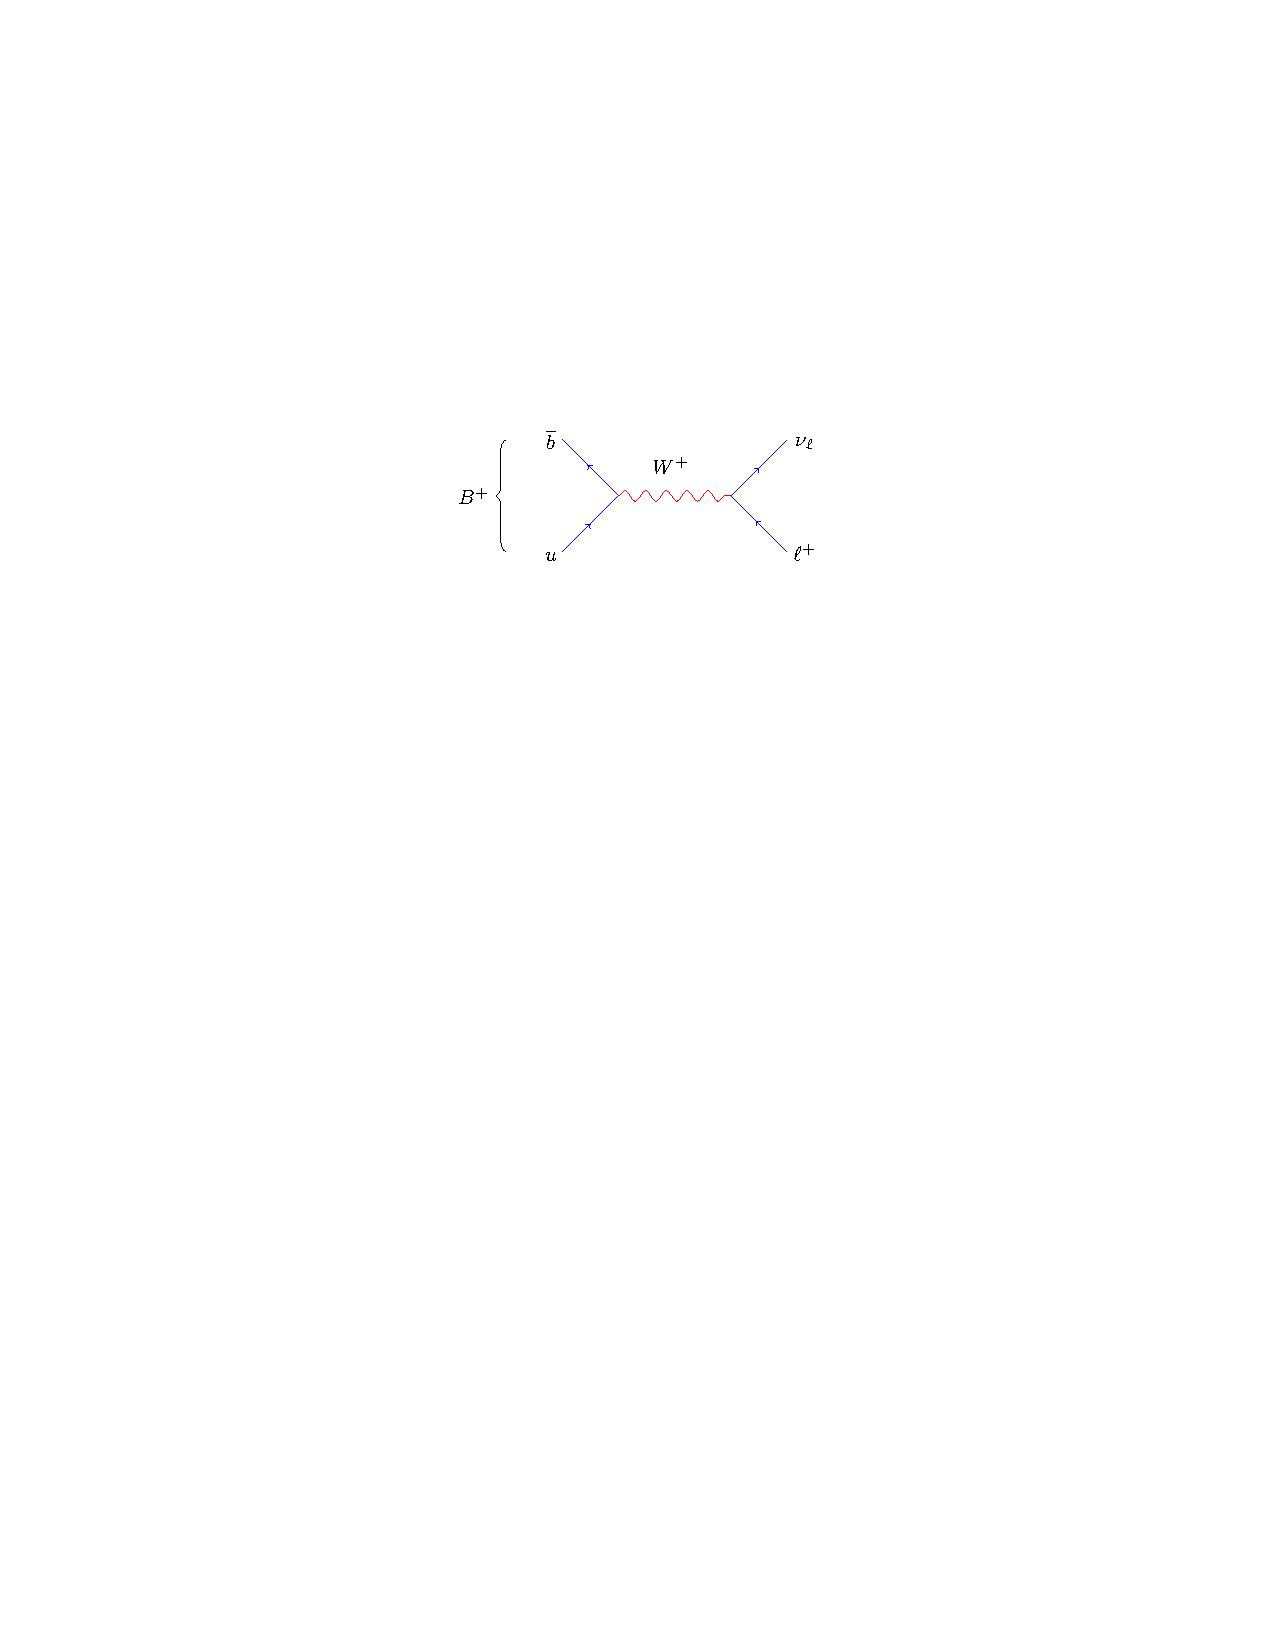
\includegraphics[width=0.5\textwidth]{figs/Theory/B2ellnu.pdf}
    \caption{Annihilation topology process for \decay{\Bp}{\ellp\neul} decays.}
    \label{fig:Theory_B2ellnu}   
\end{figure}
%%%%%%%%%%%%%%%%%%%%%%%%%%%%%%%%%%%%%%%%%%%%%%%%%%%%%%%%%%

\begin{table}[h]
   \begin{center}
      \begin{tabular}{lcc}
         \hline

         Decay Mode                 & SM prediction & Measurement \\
         \hline 
         \decay{\Bp}{\ep\neue}      & $(1.3\pm0.4)\times10^{-11}$           & $<9.8\times10^{-7}$\\
         \decay{\Bp}{\mup\neum}     & $(5.6\pm0.4)\times10^{-7}$            & $<1.0\times10^{-6}$\\
         \decay{\Bp}{\taup\neut}    & $(0.75^{+1.0}_{-0.05} )\times 10^{-4}$& $(1.09\pm0.24)\times 10^{-4}$ \\

         \hline
      \end{tabular}
   \end{center}
   \caption{Theoretical predictions and experimental measurements for \decay{\Bp}{\ellp\neul} processes, from Refs.~\cite{PhysRevD.92.051102,PhysRevD.79.091101,SATOYAMA200767}.}
   \label{tab:Theory_B2ellnu}
\end{table}
This purely leptonic \Bp meson decay can proceed to either of the three generations with the branching fractions detailed in Table~\ref{tab:Theory_B2ellnu}. The effect of helicity suppression in the final state is illustrated by the rapid decrease in predicted branching fraction as the mass charged lepton decreases. The neutrino in the final state makes this decay experimentally challenging to reconstruct at hadron colliders such as the \lhc. The measurement of \decay{\Bp}{\taup\neut} was performed at the \belle experiment, a \B-factory colliding \ep\en pairs at the $\PUpsilon(\text{4S})$ resonance. 
Hadronic annihilation decays are necessarily more complicated than these purely leptionic processes as the quark and antiquark must be further hadronised as they cannot remain bare.


{\color{Red}
\begin{itemize}
\item Talk about \D and other annihilation topologies 
\item Find origin of hadronic uncertainties 
\item \decay{\Bz}{\Kp\Km}? penguin annihilation
\end{itemize}}


\subsection{Pure annihilation topology decays}
Pure annihilation topology decays are an interesting subset of processes in which (at lowest order) only annihilation decay diagrams contribute. These are of particular interest because this allows the magnitudes of these processes to be isolated. Additionally, they provide a suitable forum in which to search for new physics; enhanced or decreased branching fractions and non-zero \CP violations are symptomatic of multiple competing processes interfering with one another.  

Typically, hadronic \emph{pure} annihilation processes are characterised by a mutually exclusive set of quarks in the initial and final state. This implies that the initial state must have completely annihilated into a mediator for this process to occur.   

{\color{Red}
\begin{itemize}
\item Pure annihilation - charmless Bc
\end{itemize}}

\subsection{Other annihilation decays}
Processes that don't uniquely proceed via annihilation decays are also of interest. 
{\color{Red}
\begin{itemize}
\item non pure - donals Bc 
\end{itemize}}

\section{Rescattering}

Rescattering allows \Bp mesons to decay to final states that are ideal pure annihilation topologies via an intermediate process of some other topology. This can potential limit the sensitivity the annihilation decay if these processes happen at a significant rate. Intermediate processes that could contribute to the \decay{\Bp}{\Dsp\phiz} decay are shown in Fig.~\ref{fig:Theory_rescattering}. These rather complicated processes both involve tree-level \decay{\bquarkbar}{\uquarkbar} transitions in which one of both of the products undergo a final state interactions.  

%%%%%%%%%%%%%%%%%%%%%%%%%%%%%%%%%%%%%%%%%%%%%%%%%%%%%%%%%%
\begin{figure}[!h]
    \centering
    \begin{subfigure}[m]{0.7\textwidth}
        \centering
        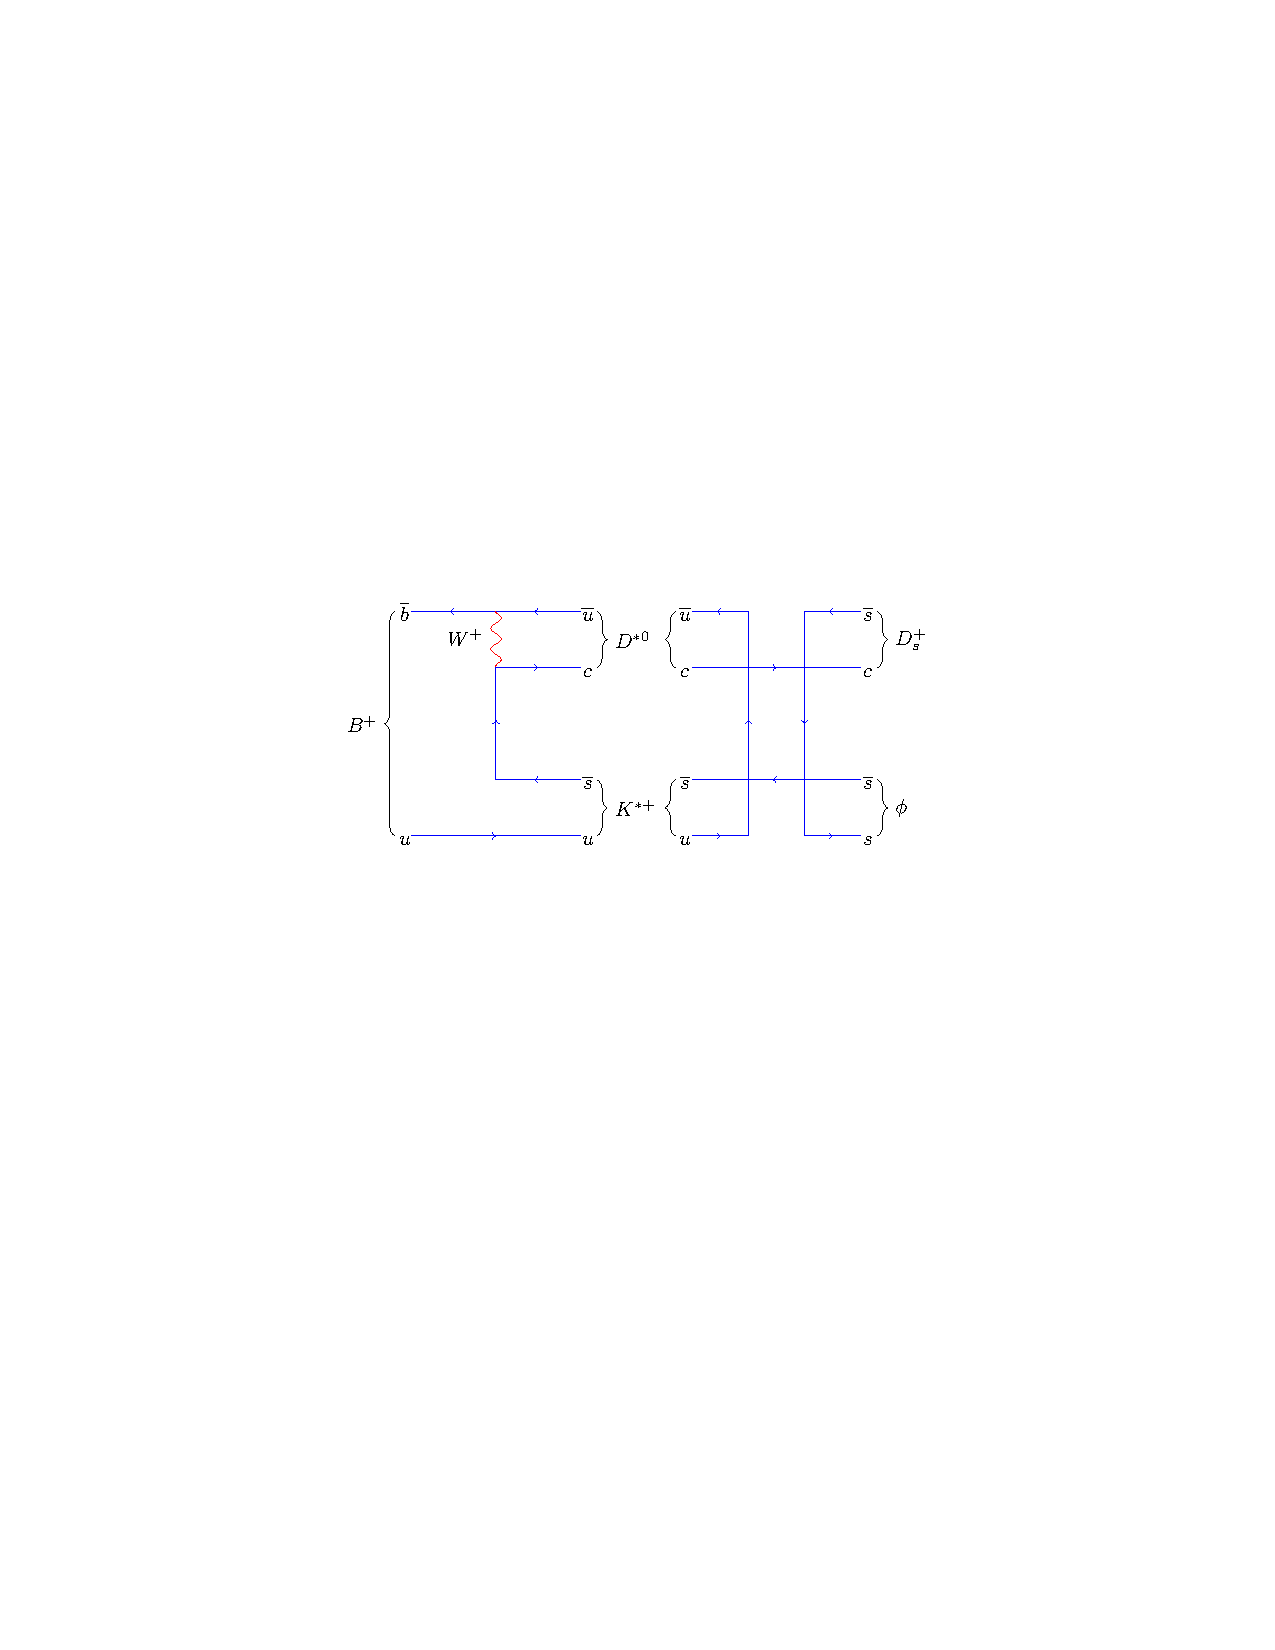
\includegraphics[width=1.0\textwidth]{figs/Theory/B2DsPhi_Rescattering_B2D0K.pdf}
        \caption{via \decay{\Bp}{\Dstarz\Kstarp}}
    \end{subfigure}
    \begin{subfigure}[m]{0.7\textwidth}
        \centering
        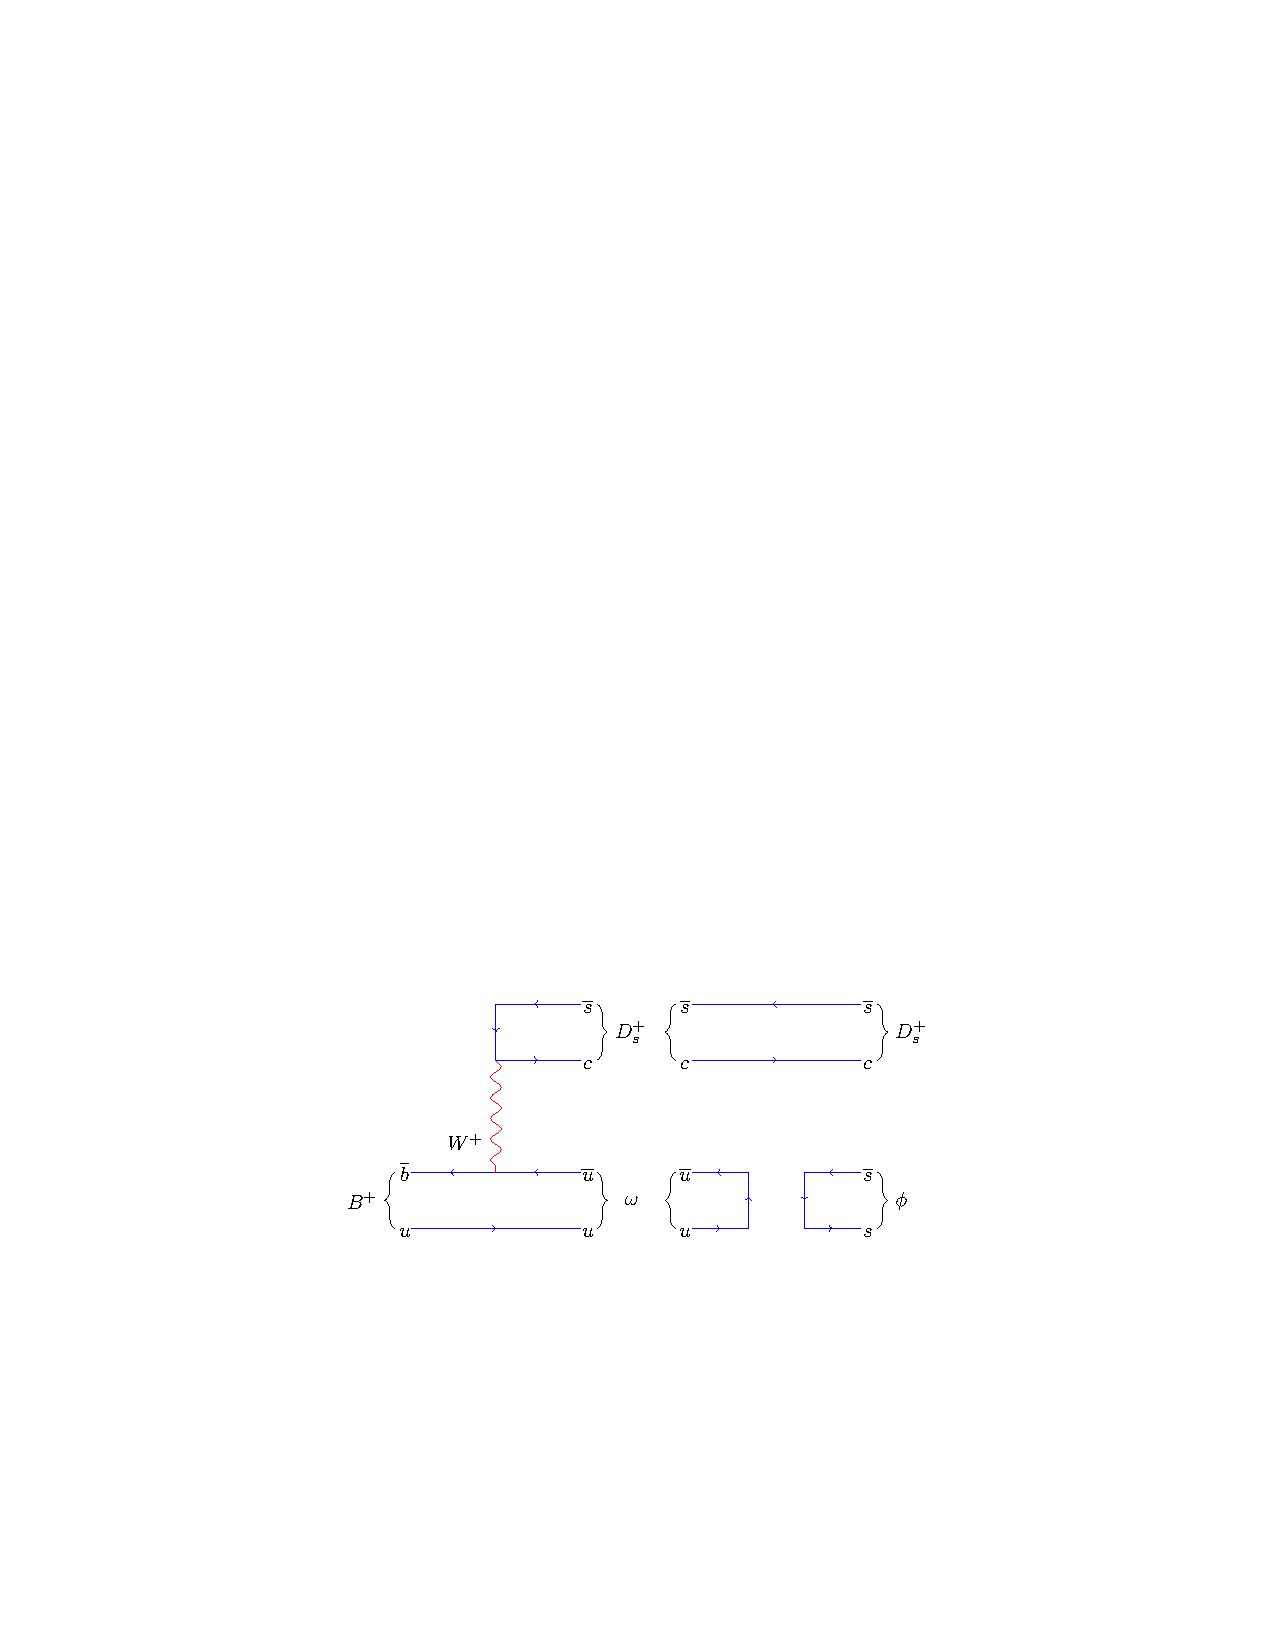
\includegraphics[width=1.0\textwidth]{figs/Theory/B2DsPhi_Rescattering_B2Dsomega.pdf}
        \caption{via $\decay{\Bp}{\Dsp\omega}$}
    \end{subfigure}
    \caption{Rescattering contributions to \decay{\Bp}{\Dsp\phiz} decays.}
    \label{fig:Theory_rescattering}   
\end{figure}
%%%%%%%%%%%%%%%%%%%%%%%%%%%%%%%%%%%%%%%%%%%%%%%%%%%%%%%%%%



{\color{Red}
\begin{itemize}
\item What is rescattering?
\item Examples of it?
\item Why it's expected to be small
\item $\decay{\Bu}{\Dsp\omega}$
\item $\omega\to\phi$ is OZI suppressed 
\item $\decay{\Bu}{\Dz\Kstarp}$
\item References: \Dp\Kstarz~\cite{Mehraban2016}.
\item $\omega - \phi$ mixing: ~\cite{OKUBO1963165,PhysRevD.79.074006}.

\end{itemize}}

\section{Theoretical predictions for the \decay{\Bp}{\Dsp\phiz} decay}

%%%%%%%%%%%%%%%%%%%%%%%%%%%%%%%%%%%%%%%%%%%%%%%%%%%%%%%%%%
\begin{figure}[!h]
    \centering
    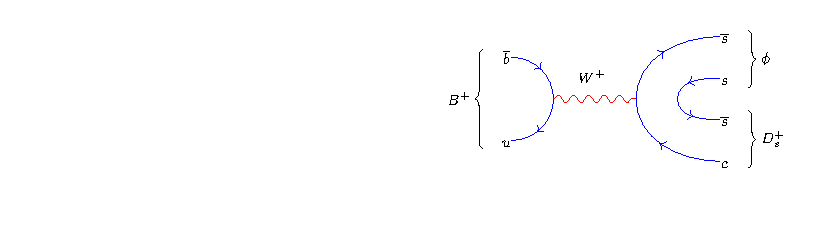
\includegraphics[width=0.6\textwidth]{figs/Theory/B2DsPhi.pdf}
    \caption{\decay{\Bp}{\Dsp\phiz} }
    \label{fig:Theory_DsPhiDiagram}   
\end{figure}
%%%%%%%%%%%%%%%%%%%%%%%%%%%%%%%%%%%%%%%%%%%%%%%%%%%%%%%%%%



{\color{Blue}
In the SM, the decay $\decay{\Bp}{\Dsp\phi}$ proceeds dominantly via the annihilation diagram shown in Fig.~\ref{fig:Theory_DsPhiDiagram}. 
This suppressed topology requires the wave functions of the incoming quarks to overlap sufficiently to annihilate into a virtual \Wp boson. 
The decay is further suppressed by the small magnitude of the CKM matrix element \Vub associated with the annihilation vertex. 


}

\subsection{Standard model predictions}
{\color{Blue}
Several SM predictions have been made for the branching fraction of the $\decay{\Bp}{\Dsp\phi}$ decay~\cite{Zou:2009zza, Mohanta:2002wf, Mohanta:2007uu, Lu:2001yz}, using input from lattice calculations~\cite{fB:2013HPQCD,fB:2016ETM, fB:2016Fermi}. These predictions are in the range $(1-7)\times10^{-7}$, where the limit on the precision is dominated by hadronic uncertainties. 

In addition, unlike many rare hadronic decays including $\decay{\Bp}{\Dsp\Kp\Km}$, possible contributions from rescattering effects are expected to be small, for example contributions from intermediate states such as $\decay{\Bp}{\Dsp\omega}$~\cite{Gronau:2012gs}.

}

{\color{Red}
\begin{itemize}
\item Find origin of hadronic uncertainties 
\end{itemize}}

\subsection{BSM models and predictions}
{\color{Blue}
However, additional diagrams contributing to this decay can arise in some extensions of the SM, such as supersymmetric models with R-parity 
violation. They could enhance the branching fraction and/or produce large \CP asymmetries~\cite{Mohanta:2002wf, Mohanta:2007uu}, which makes the $\decay{\Bp}{\Dsp\phi}$ decay a promising place to search for new physics beyond the SM.\footnote{Charge conjugation is implied throughout this paper. Furthermore, $\phi$ denotes the $\phi(1020)$ resonance.}
}

{\color{Red}
\begin{itemize}
\item Higgs doublet
\item SUSY 
\item include feynman diagrams
\item small intro into models
\end{itemize}}

\subsection{Previous measurements}

{\color{Blue}
The \lhcb experiment reported evidence for the decay $\decay{\Bp}{\Dsp\phi}$ using $pp$ collision data corresponding to an integrated luminosity of 1\invfb taken during 2011, at a centre-of-mass energy of 7\tev~\cite{Aaij:2012zh}. A total of $6.7^{+4.5}_{-2.6}$ candidates was observed. The branching fraction was determined to be 

\begin{equation}
\mathcal{B}(\decay{\Bp}{\Dsp\phi}) = (1.87^{+1.25}_{-0.73} \pm 0.19 \pm 0.32) \times 10^{-6},
\end{equation}
where the first uncertainty is statistical, the second is systematic and the third is due to the uncertainty on the branching fraction of the decay $\decay{\Bp}{\Dsp\Dzb}$, which was used as normalisation. 
Given the large uncertainties on both the theoretical and experimental values, the previously measured value is consistent with the range of SM values given above.
}

{\color{Red}
\begin{itemize}
\item Include plot and measurement
\item say something about similarites 
\end{itemize}}


\section{Theoretical predictions for the \decay{\Bp}{\Dsp\Kp\Km} decay}


%%%%%%%%%%%%%%%%%%%%%%%%%%%%%%%%%%%%%%%%%%%%%%%%%%%%%%%%%%
\begin{figure}[!h]
    \centering
    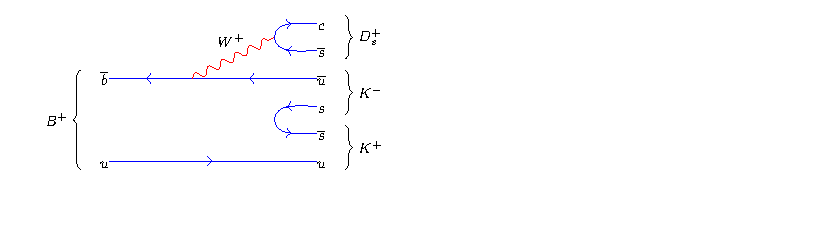
\includegraphics[width=0.6\textwidth]{figs/Theory/B2DsKK.pdf}
    \caption{\decay{\Bp}{\Dsp\Kp\Km} }
    \label{fig:Theory_DsKKDiagram}   
\end{figure}
%%%%%%%%%%%%%%%%%%%%%%%%%%%%%%%%%%%%%%%%%%%%%%%%%%%%%%%%%%



{\color{Blue}
The decay $\decay{\Bp}{\Dsp\Kp\Km}$ is mediated by a $\decay{\bquarkbar}{\uquarkbar}$ transition shown in Fig.~\ref{fig:Theory_DsKKDiagram} and is therefore suppressed in the Standard Model (SM) due to the small size of the Cabibbo-Kobayashi-Maskawa (CKM) matrix element \Vub. 
}


{\color{Red}
\begin{itemize}
\item explain what a dalitz plot is
\end{itemize}
}

\subsection{Standard model predictions}
{\color{Blue}
The branching fraction for this decay is currently not measured, however a similar decay, \decay{\Bp}{\Dsp \piz}, has been observed with a branching fraction of $\mathcal{B}(\decay{\Bp}{\Dsp \piz}) = (1.5 \pm 0.5) \times 10^{-5}$~\cite{Aubert:2006xy}.
}


{\color{Red}
\begin{itemize}
\item talk about \decay{\Bp}{\Dsp\piz}
\item Could talk about \decay{\Bp}{\Dp\Kp\pim} and estimate   
\end{itemize}}

\subsection{Previous measurements}




\chapter{The \lhcb experiment} 
\label{ch:detector}
\minitoc
 


\section{\cern and the \lhc}


In the aftermath of the Second World War a number of eminent scientists proposed the creation of a collaborative European laboratory dedicated to the study of atomic physics. With this the `Conseil Europ\'een pour la Recherche Nucl\'eaire' was born; a provisional council set up in 1952 to oversee the laboratory's creation.  In 1954 the organisation as it is today was established, named the `Organisation Europ\'eenne pour la Recherche Nucl\'eaire', although the acronym \cern remained. 
The purpose of \cern was clear; the convention dictates that the organisation \emph{`shall provide for collaboration among European States in nuclear research of a pure scientific and fundamental character'}.
As such 

Furthermore, the convention stipulates that the organisation \emph{`shall have no concern with work for military requirements'} and  
requires \emph{`the results of its experimental and theoretical work shall be published or otherwise made generally available'}. 
The choice of the laboratories location followed a similar set of values, picking Geneva in Switzerland owing both to the central European location and neutrality of the host state. 


Perhaps the most well known accelerator in the complex [cite something], \cern is home to the Large Hadron Collider (\lhc). Two beams of hadrons circulate in opposite directions around 27\km rings, colliding at four interaction points. The beam pipes and experimental halls are buried deep underground, providing shielding from radiation and reducing the cost of acquiring large areas of land. The tunnels traverse the Franco-Swiss border at a depth that varies between 50--175\m at the lowest and highest points respectively.      


{\color{Red}
\begin{itemize}
\item Founding of \cern and a little history 
\item LEP was in tunnel before
\item Mission statement
\item Notable results and and contributions to society
\item Mention experiments other than those attached to accelerator complex
\item Time line
\item running periods? and future plans...
\end{itemize}
}

\subsection{The accelerator complex}

The \lhc is only one of a vast collection of accelerators at \cern, albeit the largest. The hadrons collided in the \lhc travel sequentially through a number of different machines, boosting their momentum in each. The full complex is shown in Fig.~\ref{fig:Dec_lhcb_Schematic} along with a legend detailing the types of particles considered. The protons begin life in a hydrogen gas canister. The gas is ionised and accelerated in  a linear accelerator, LINAC2, to an energy of 50\mev. These then pass into the Proton Synchrotron Booster, raising the energy further from 50\mev to 1.4\gev. 

In addition to protons, the complex can accelerate other ions including lead, and more recently, argon and xenon {\color{Red}cite}. These start in a dedicated linear accelerator, LINAC3, where the ions are stripped to bare nuclei before being injected into the Low Energy Ion Ring (LEIR). This ring raises the ion's energy from 4.2\mev to 72\mev. 

Either protons or ions can then be injected in the Proton Synchrotron (PS), \cern's first synchrotron. Once the world's highest energy particle accelerator, this now accelerates the particles up to 25\gev ready to be injected into the Super Proton Synchrotron (SPS).
The SPS is the second largest accelerator at \cern, with a circumference of 7\km. It was switched on in 1976 and resulted in the notable discoveries of the \W and \Z bosons. Here, the particles are accelerated up to an energy of 450\gev. 

%%%%%%%%%%%%%%%%%%%%%%%%%%%%%%%%%%%%%%%%%%%%%%%%%%%%%%%%%%
\begin{figure}[!h]
    \centering
    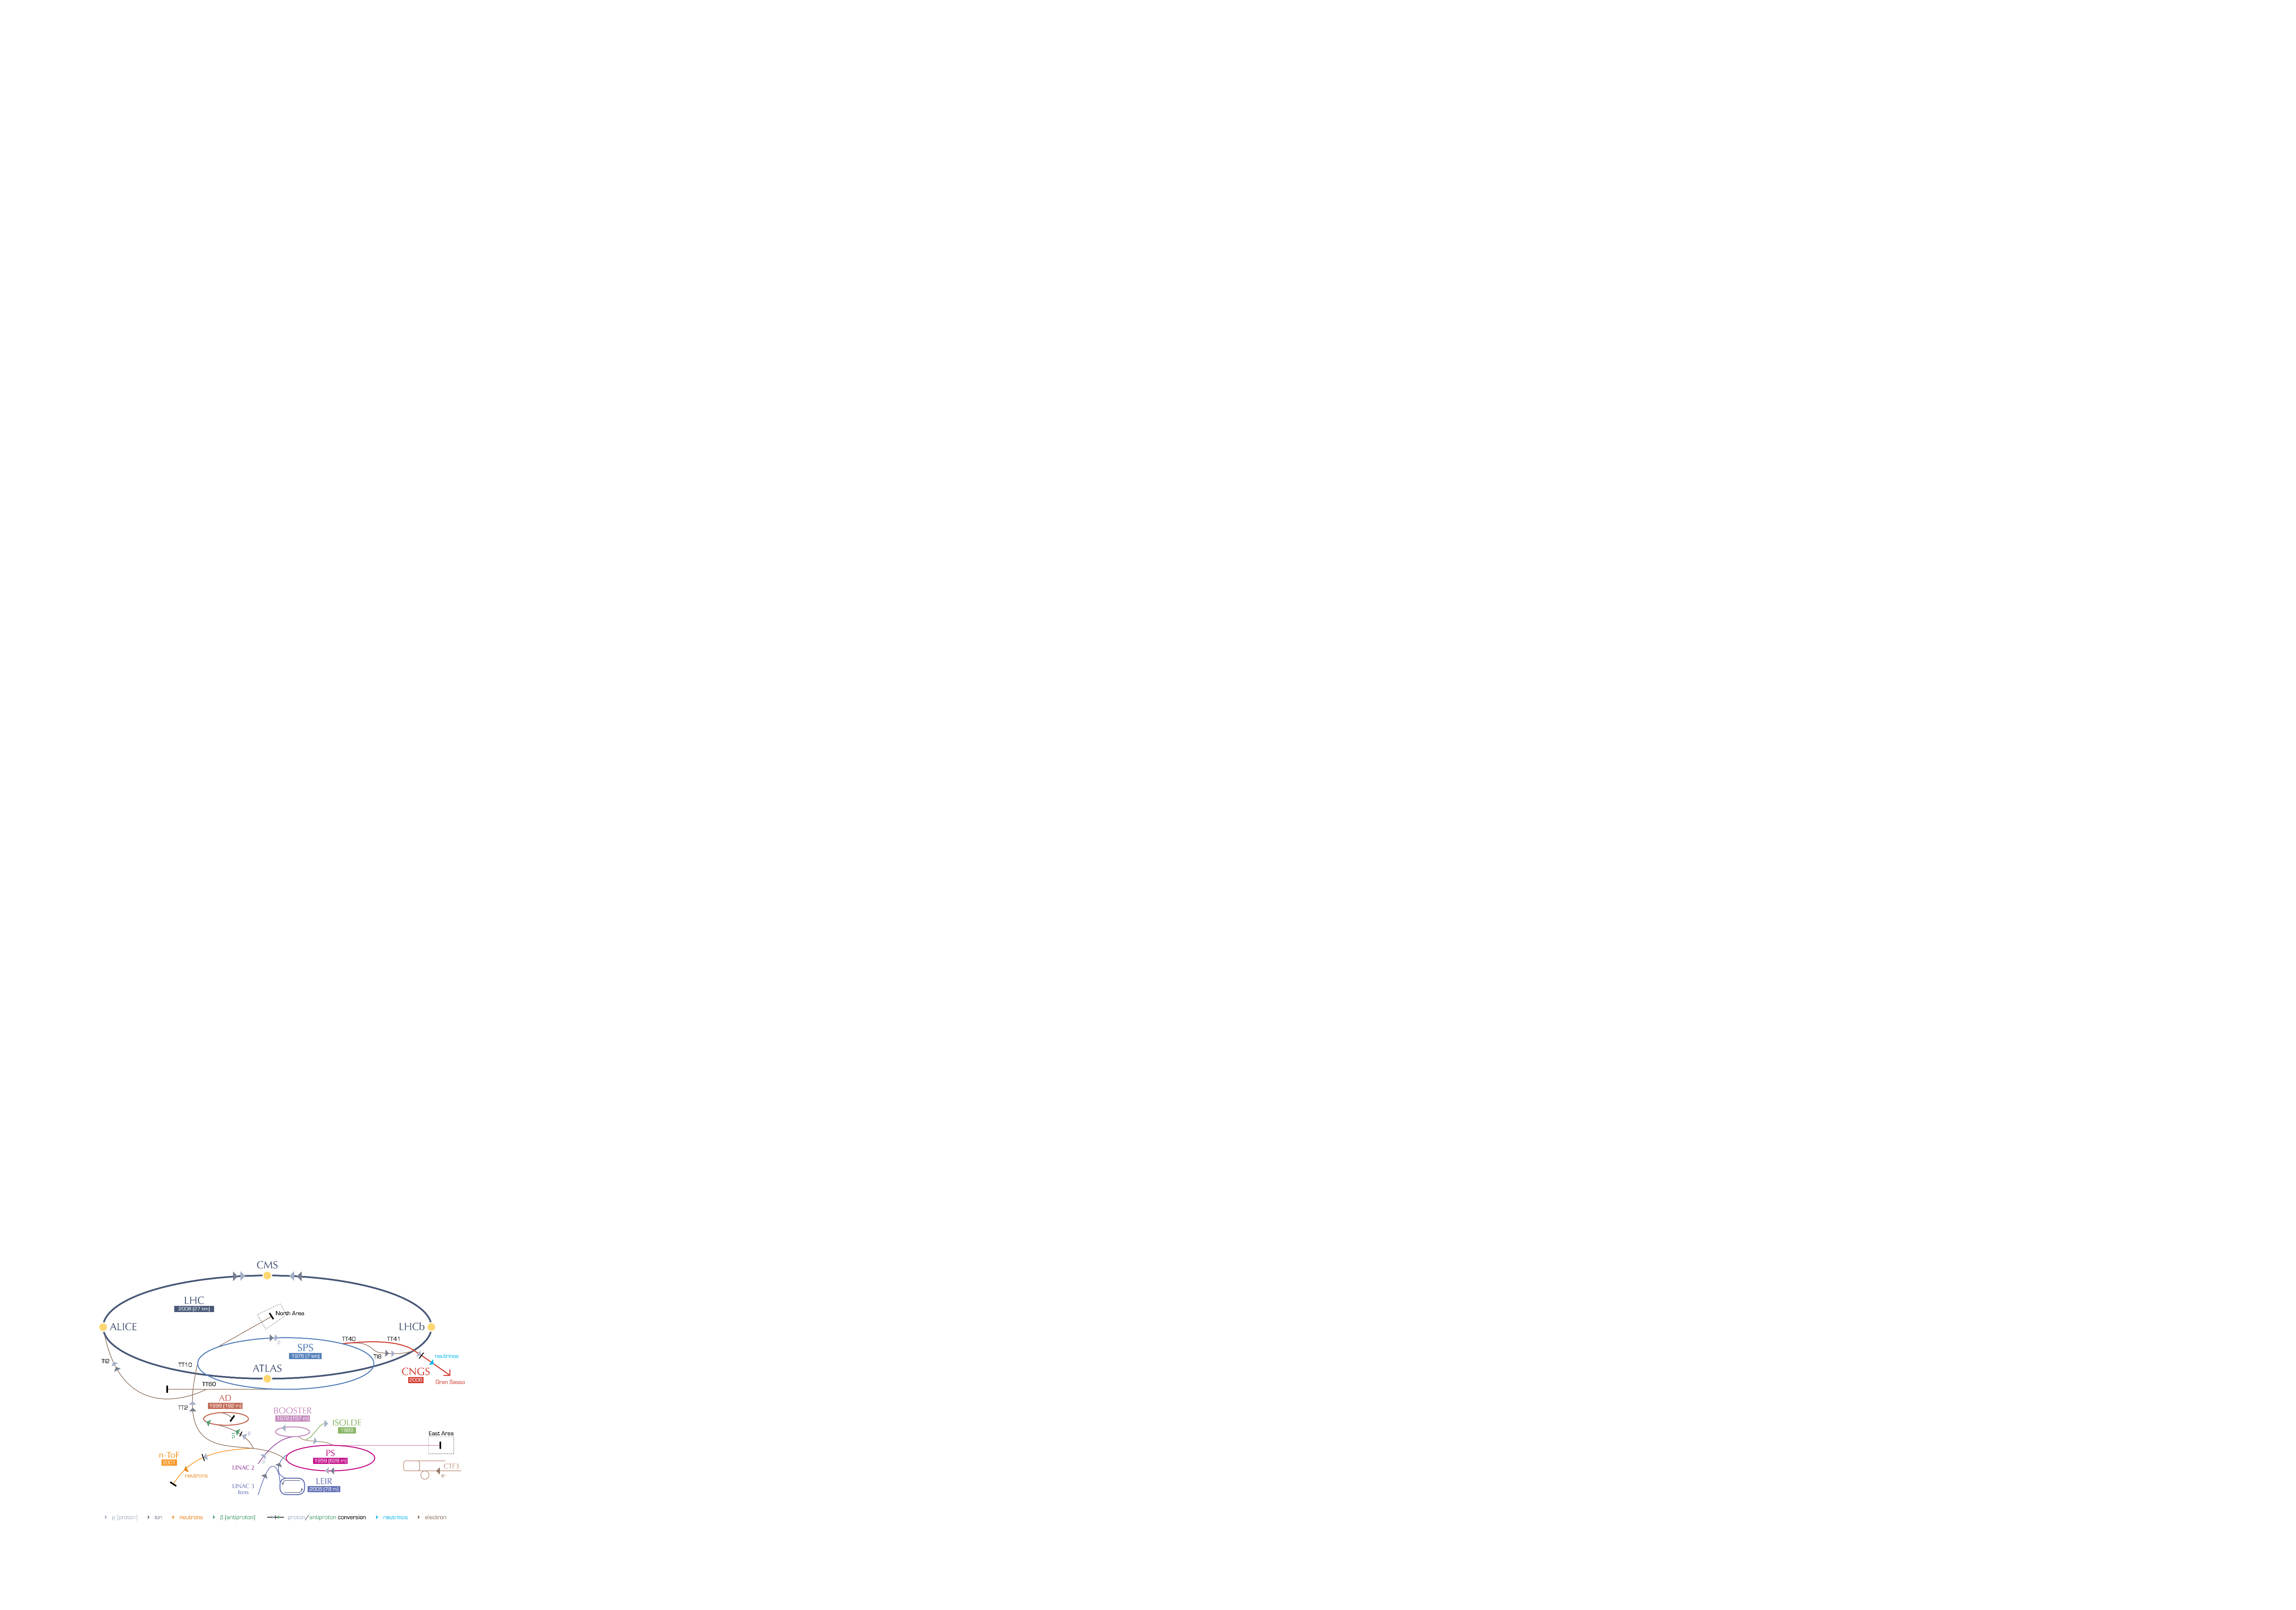
\includegraphics[width=1.0\textwidth]{figs/Detector/Acc_complex.pdf}
    \caption{The accelerator complex at \cern taken from Ref...}
    \label{fig:Dec_Acc_Complex}   
\end{figure}
%%%%%%%%%%%%%%%%%%%%%%%%%%%%%%%%%%%%%%%%%%%%%%%%%%%%%%%%%%



{\color{Red}
\begin{itemize}
\item Brief overview of the life of a proton from source to \lhc
\item injected into two beams
\item injection points
\item Phases of \lhc?
\end{itemize}
}

\subsection{The \lhcb collaboration} 
A total of seven experiments are located at the \lhc, situated in four caverns. The four largest are \atlas, \cms, \lhcb and \alice. The TOTEM, LHCf and MoDEL experiments are located in the same caverns as \cms, \atlas and \lhcb respectively. 

The \lhcb collaboration is made up of around 800 scientists 


{\color{Red}
\begin{itemize}
\item People and counties 
\item physics aims?
\end{itemize}
}
\subsection{Beam conditions at \lhcb}
{\color{Red}
\begin{itemize}
\item \lhc optics
\item crossing angle
\item Luminosity levelling
\end{itemize}
}


\section{The \lhcb detector}

This section provides an overview of the experimental apparatus used to obtain the data analysed in this thesis.
The \lhcb detector is comprised of distinct sub-detectors, each with a dedicated purpose. These help to characterise the sub-atomic particles created in the proton-proton collisions, and enable measurements of their kinematics, trajectories and species.
This overview includes a description of the sub-detector's construction, components and performance. 

The \lhcb detector is found at Point 8 of the \lhc ring, a cavern originally built for the {\color{Red}\delphi} detector during the \lep era. A schematic representing the key components of the \lhcb detector is shown in Fig.~\ref{fig:Dec_lhcb_Schematic}. This figure displays the axes convention adopted by \lhcb, and used henceforth. The horizontal axis is labelled the $z$-axis and is parallel to the direction of the beams. The figure's vertical axis is the $y$-axis, increasing as one moves from the cavern up to ground level. The $x$-axis is in the dimension perpendicular to the plane of the figure. The $x$-axis increases as one moves towards the centre of the \lhc ring. The counter-rotating beams of protons are collided at the far left of this figure, at the origins of the $y$- and $z$-axes.   

%%%%%%%%%%%%%%%%%%%%%%%%%%%%%%%%%%%%%%%%%%%%%%%%%%%%%%%%%%
\begin{figure}[!h]
    \centering
    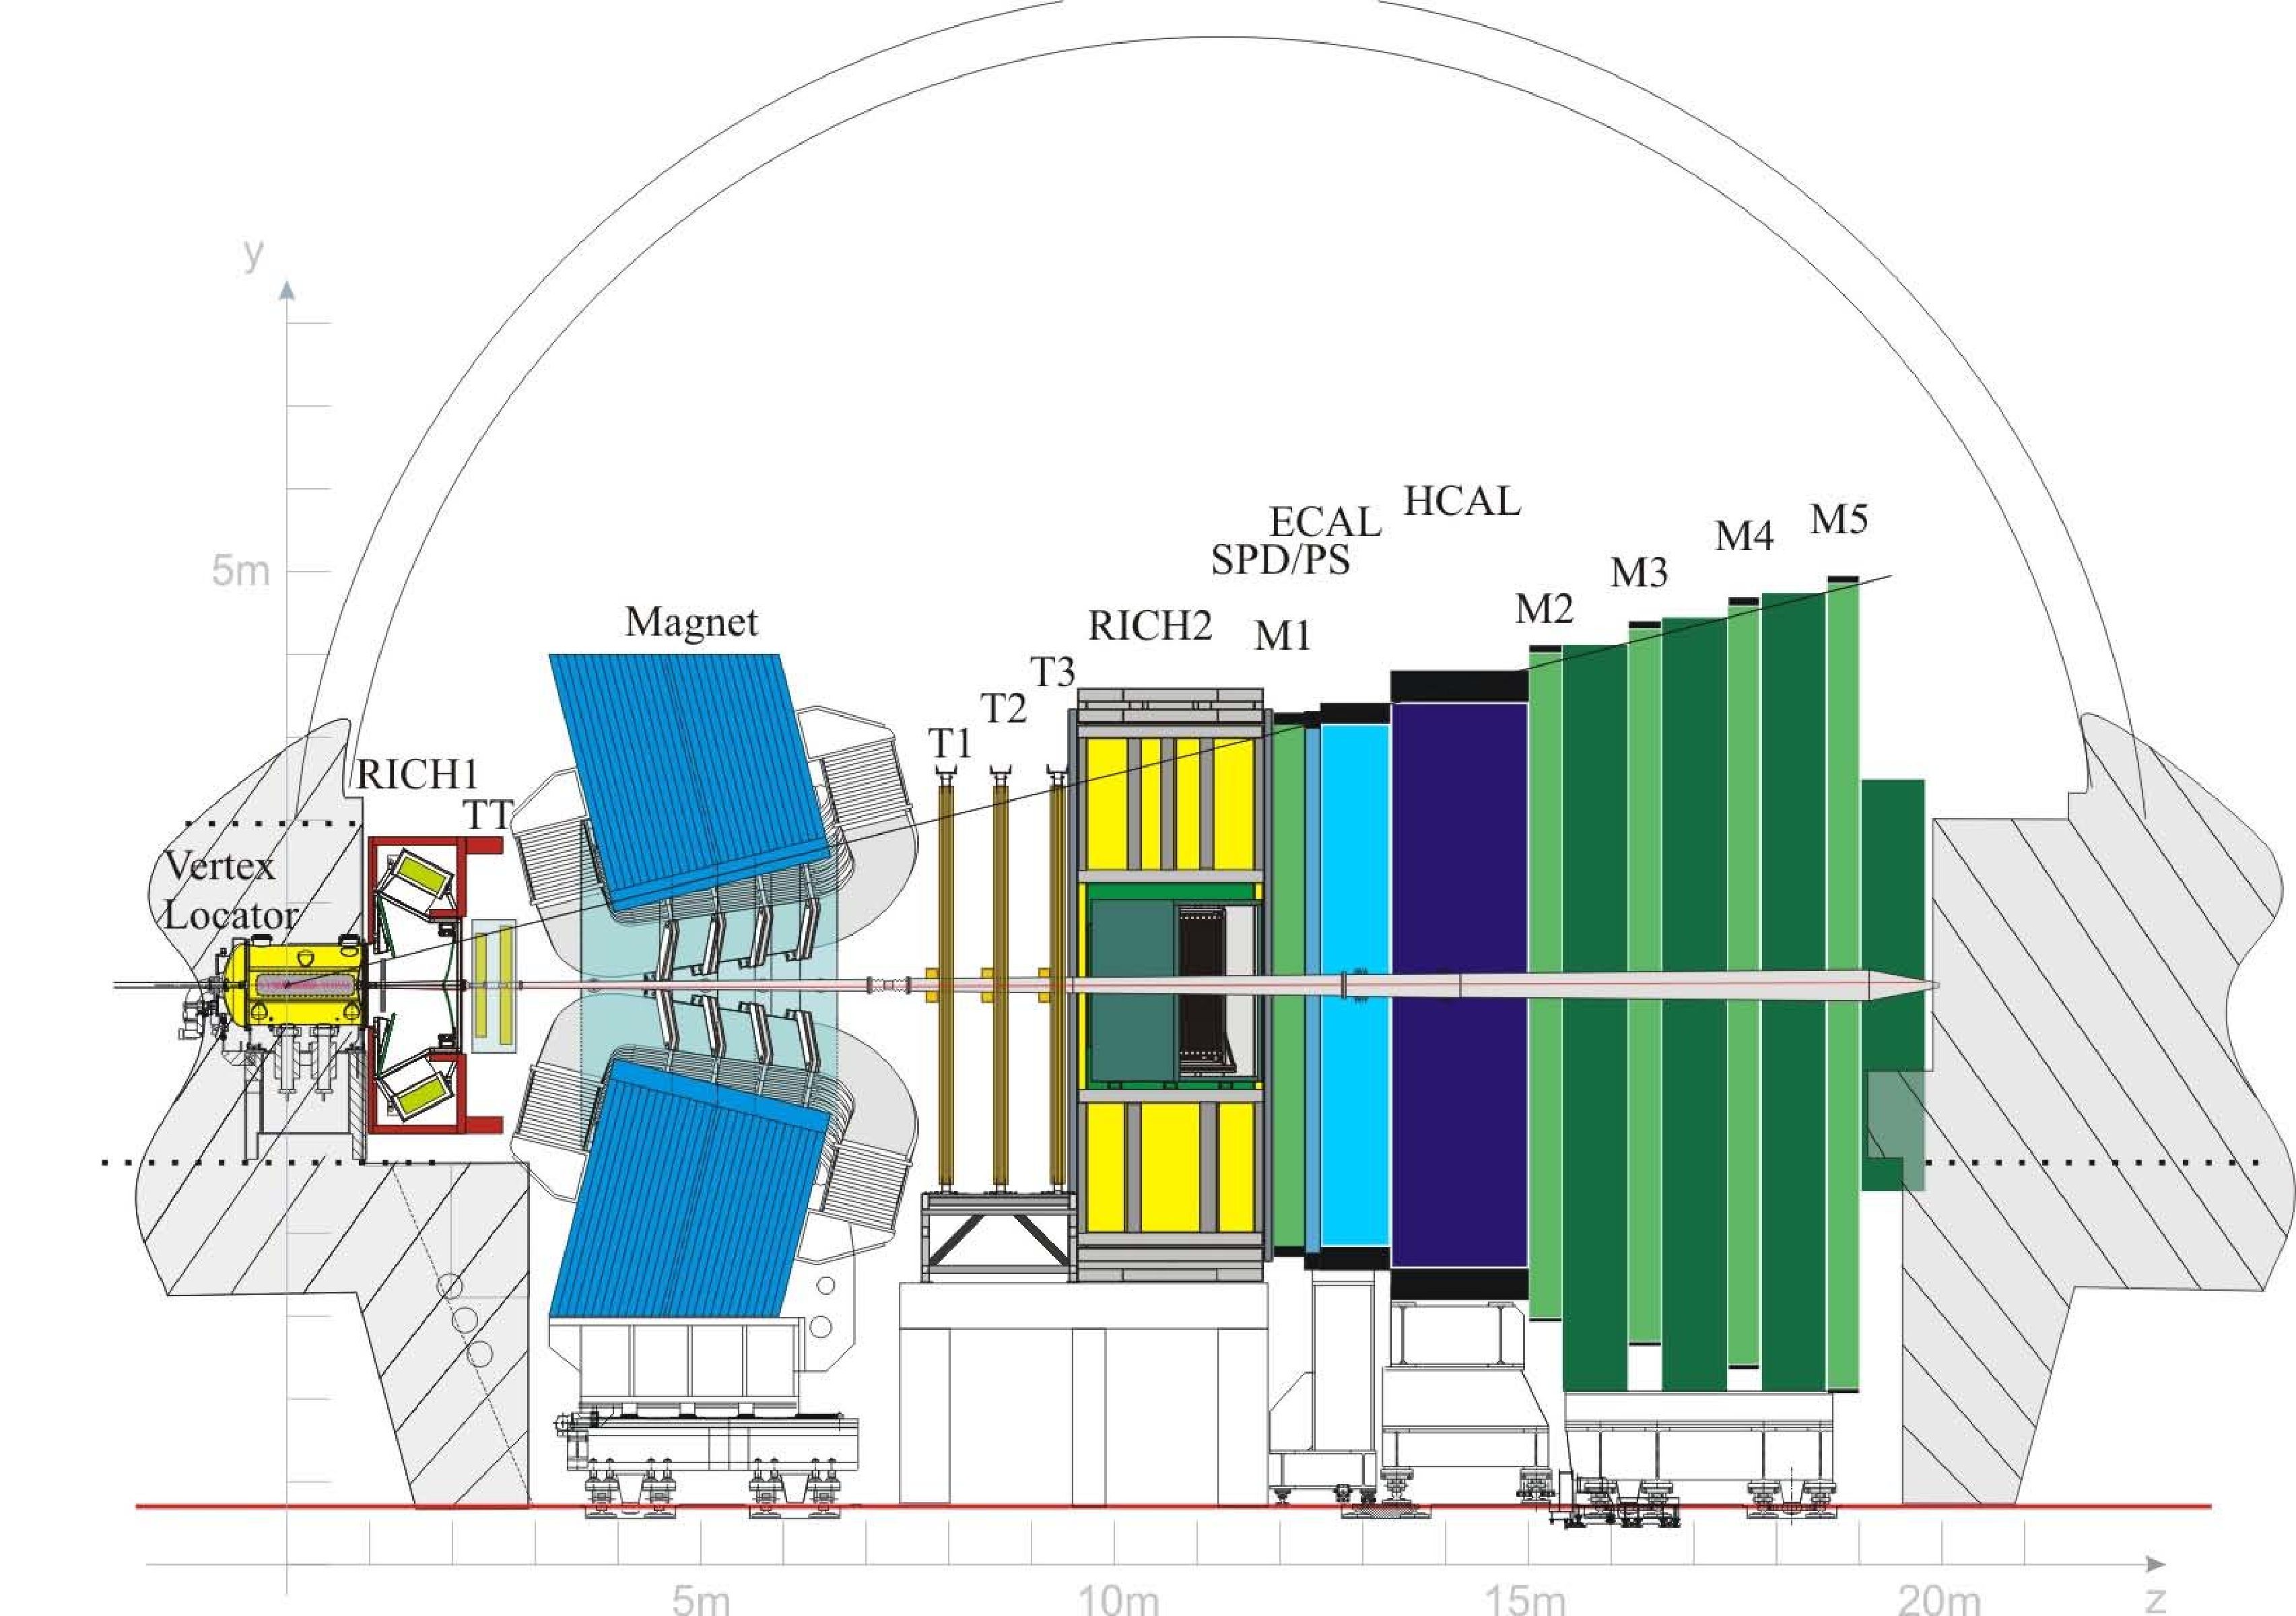
\includegraphics[width=0.8\textwidth]{figs/Detector/LHCb_Detector_Schematic.pdf}
    \caption{Schematic of the \lhcb detector, from Ref.~\cite{Alves:2008zz}.}
    \label{fig:Dec_lhcb_Schematic}   
\end{figure}
%%%%%%%%%%%%%%%%%%%%%%%%%%%%%%%%%%%%%%%%%%%%%%%%%%%%%%%%%%



Running along the centre of the detector is the \lhcb beampipe. The primary role is to separate the inner vacuum chamber from the rest of the cavern, allowing the beams to proceed unimpeded by the air. The majority of the beampipe is made of beryllium, with smaller sections made out of aluminium alloys or stainless steel. Although beryllium is a highly toxic and fragile material it has a long radiation length, allowing the incident particles to traverse the pipe walls with minimal interactions.  


{\color{Green}
\begin{itemize}
\item Distribution of bb pairs
\end{itemize}
}

\subsection{Magnet}

The \lhcb detector contains a warm dipole magnet that bends the trajectories of charges particles, allowing measurements of the particles' momentum. The magnet has two saddle-shaped coils inside a square yoke that generate an integrated magnetic field of 4 Tm.  
The magnetic field is aligned along the $y$-axis, bending the charged particles in the horizontal plane. The polarity of the magnetic is routinely switched during data taking. This helps to understand and cancel systematic effects that may affect measurements of \CP asymmetries. The two magnet polarities are referred to \emph{MagDown} and \emph{MagUp}, corresponding to a field in the negative and positive $y$-axis direction respectively.   

A schematic of the magnet is shown in Fig.~\ref{fig:Dec_magnet}, along with the strength of the magnetic field as a function of the $z$-axis position. Both magnet polarities are represented in this figure. 

{\color{Red}
\begin{itemize}
\item Magnet: purpose and design 
\end{itemize}
}


%%%%%%%%%%%%%%%%%%%%%%%%%%%%%%%%%%%%%%%%%%%%%%%%%%%%%%%%%%
\begin{figure}[!h]
    \centering
    \begin{subfigure}[t]{0.4\textwidth}
        \centering
        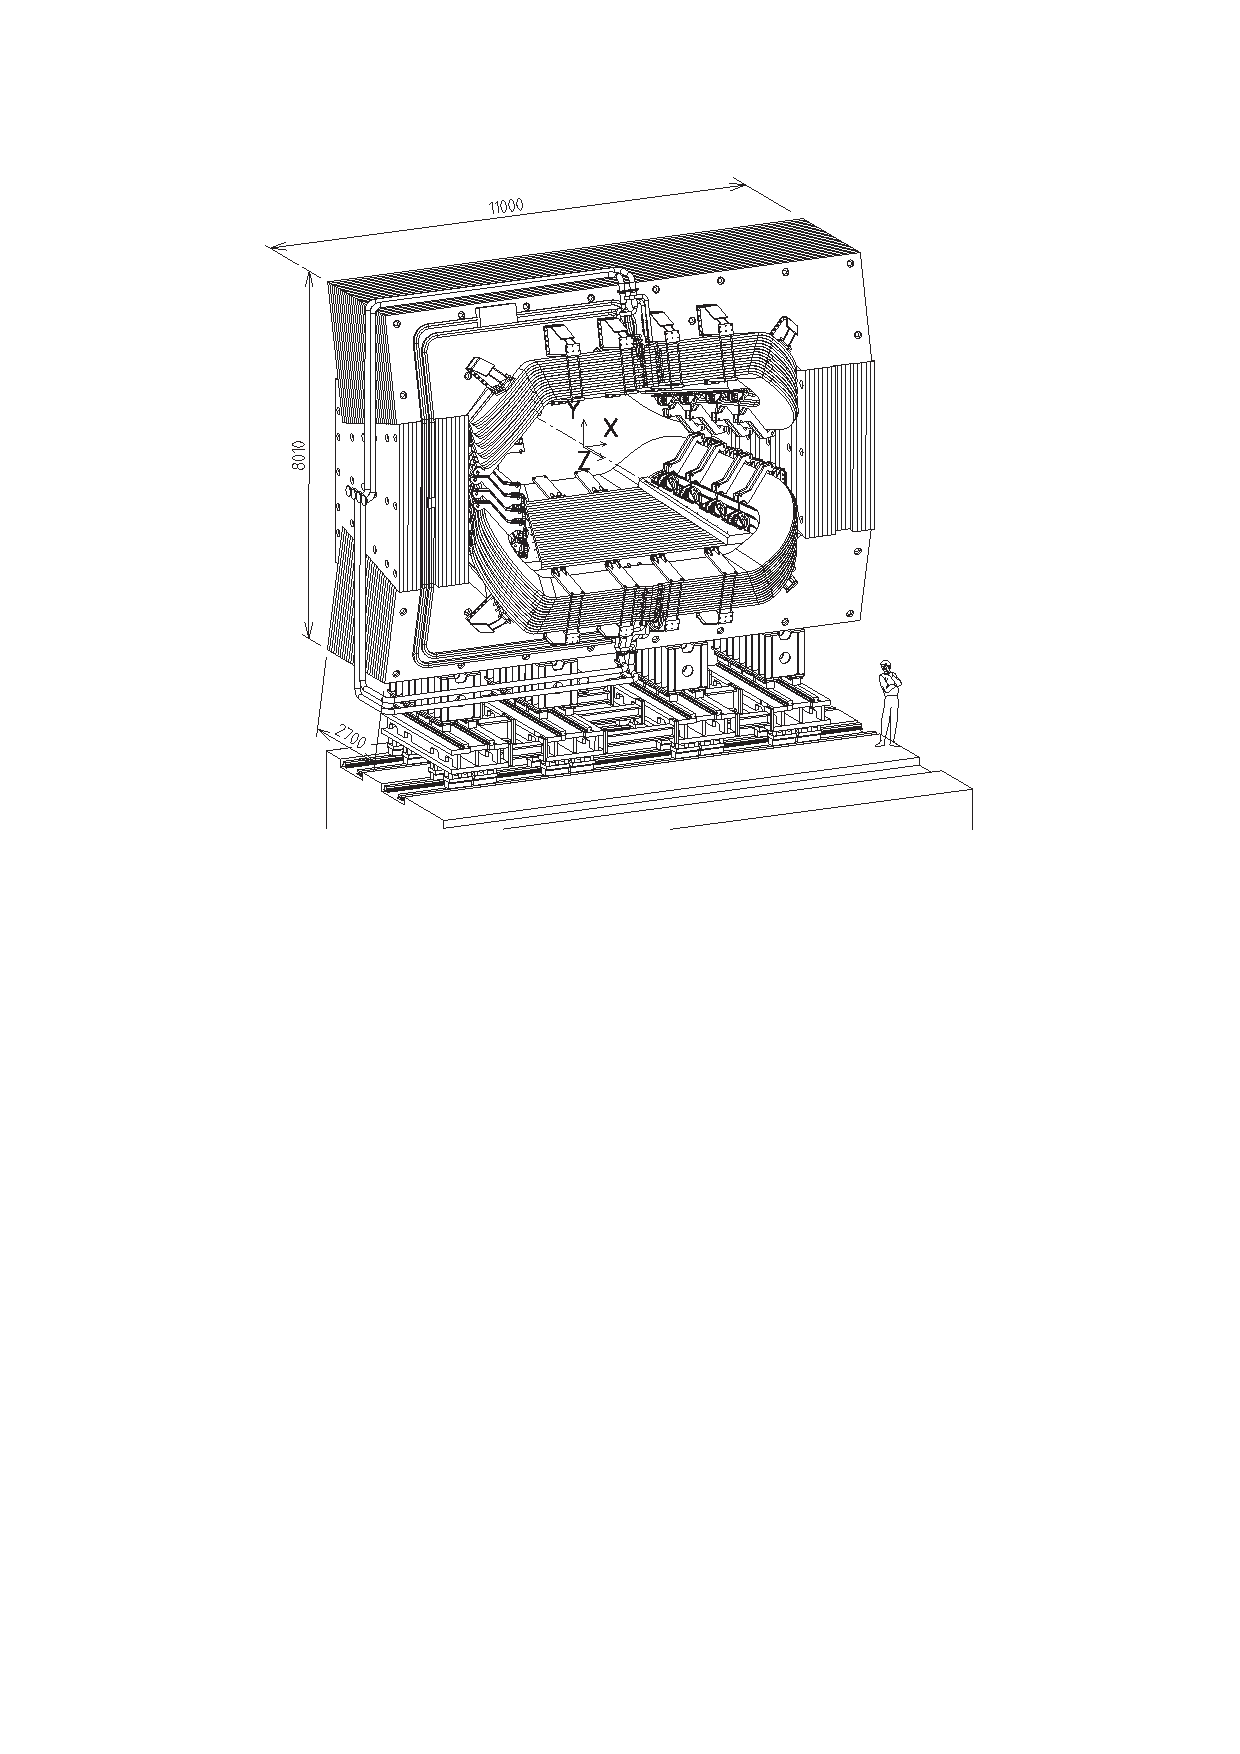
\includegraphics[width=1.0\textwidth]{figs/Detector/magnet_schematic.pdf}
    \end{subfigure}
    \begin{subfigure}[t]{0.4\textwidth}
        \centering
        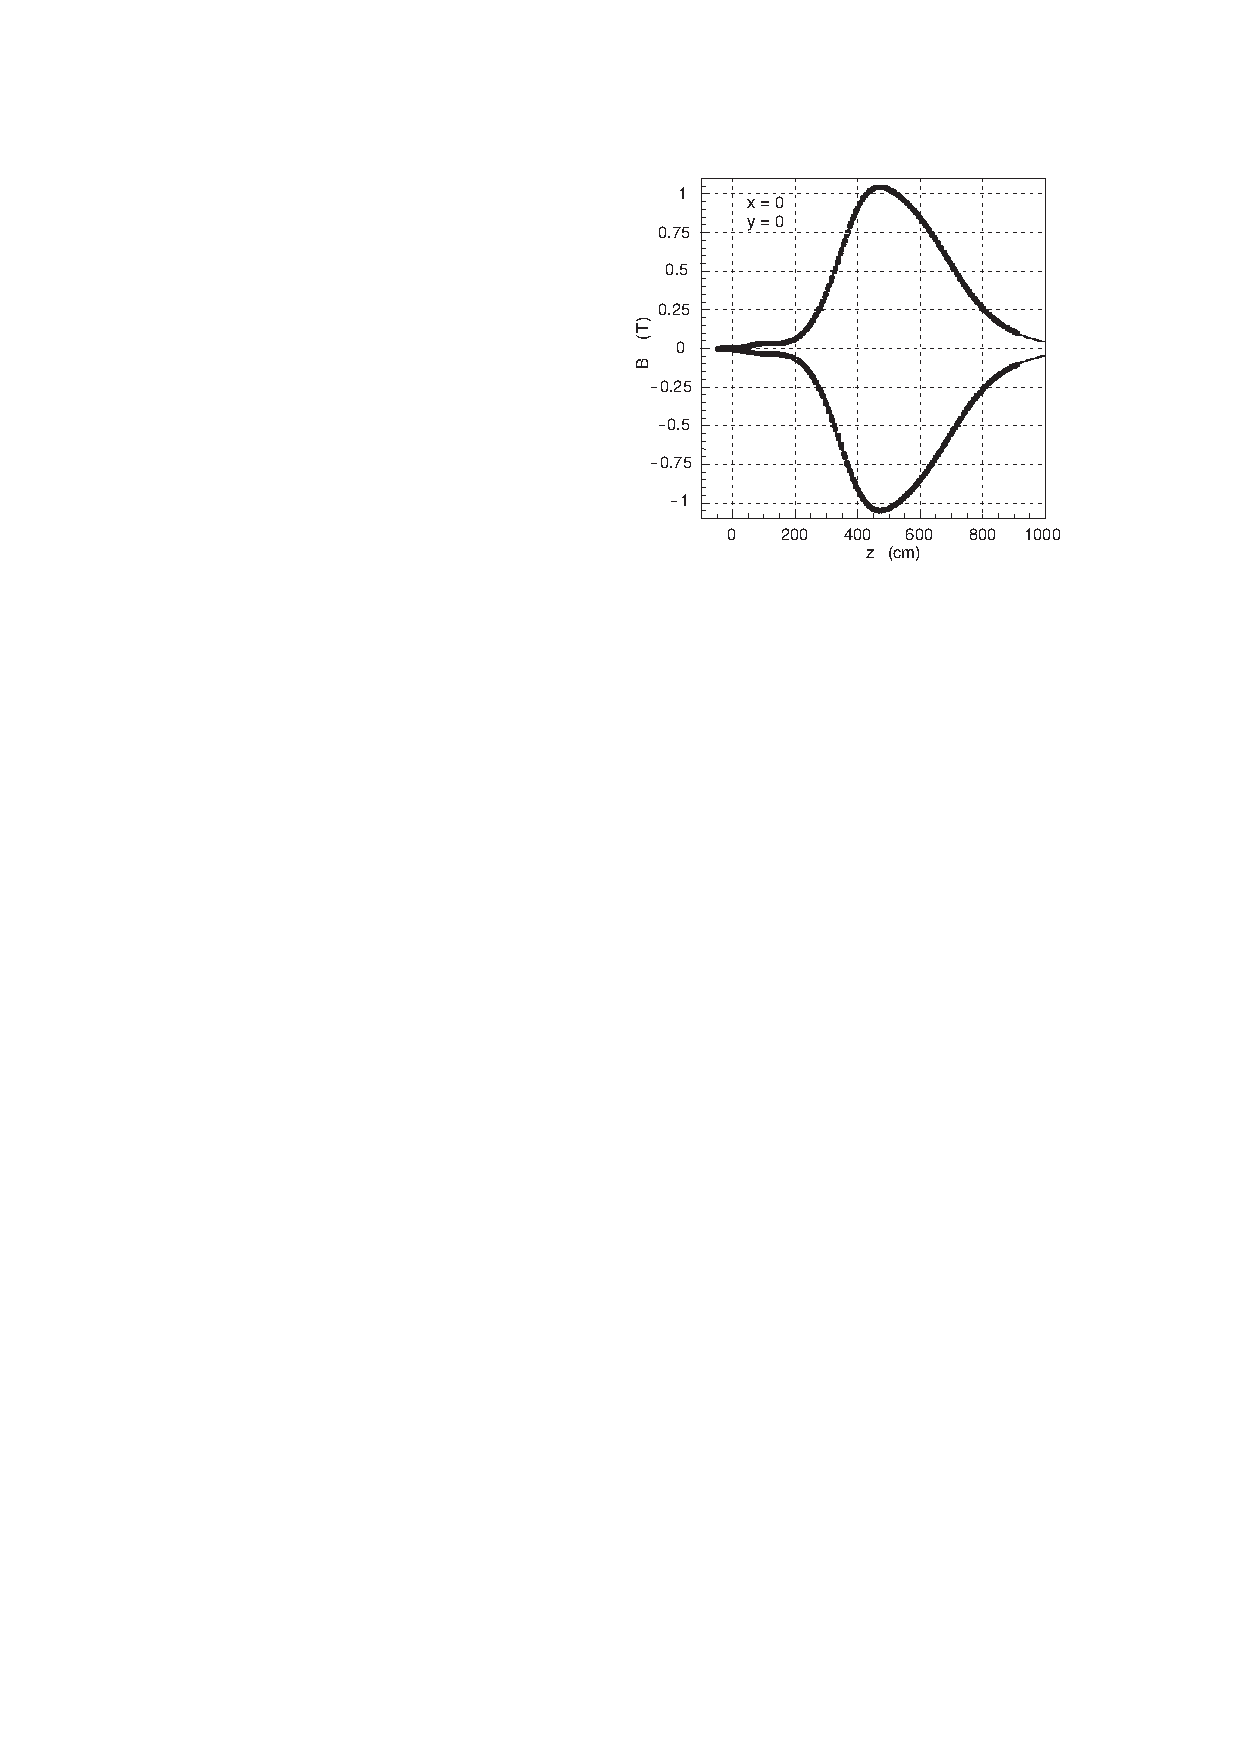
\includegraphics[width=1.0\textwidth]{figs/Detector/magnet_B_field.pdf}
    \end{subfigure}
    \caption{Schematic of the \lhcb warm dipole magnet (left) and the magnetic field strength along the $z$-axis (right) from Ref.~\cite{Alves:2008zz}.}
    \label{fig:Dec_magnet}   
\end{figure}
%%%%%%%%%%%%%%%%%%%%%%%%%%%%%%%%%%%%%%%%%%%%%%%%%%%%%%%%%%


\subsection{Vertex Locator}

The first sub-detector to make measurements of the particles produced in proton-proton collisions is the Vertex Locator (\velo) encompassing the collision region. This sub-detector make precise measurements of the track positions of charged particles as they emanate out of the collisions. A high level of precision is required to identify the secondary vertices characteristic of \bquark- and \cquark-hadron decays. These secondary vertices are typically displaced from the interaction position as a result of the long lifetimes associated to these heavy-flavour hadrons. This is achieved by measuring the track coordinates using silicon sensors placed a close to the \lhc beam as safety allows. The \velo sensors are semicircular devices placed on either side of the beam. To allow the sensors to instrument the innermost region around the interaction point the two halves of the \velo can move horizontally in and out. During normal data taking this allows the sensors to be 7\mm away from the interaction point yet still be a safe distance away from the beams at injection. 

%%%%%%%%%%%%%%%%%%%%%%%%%%%%%%%%%%%%%%%%%%%%%%%%%%%%%%%%%%
\begin{figure}[!h]
    \centering   
    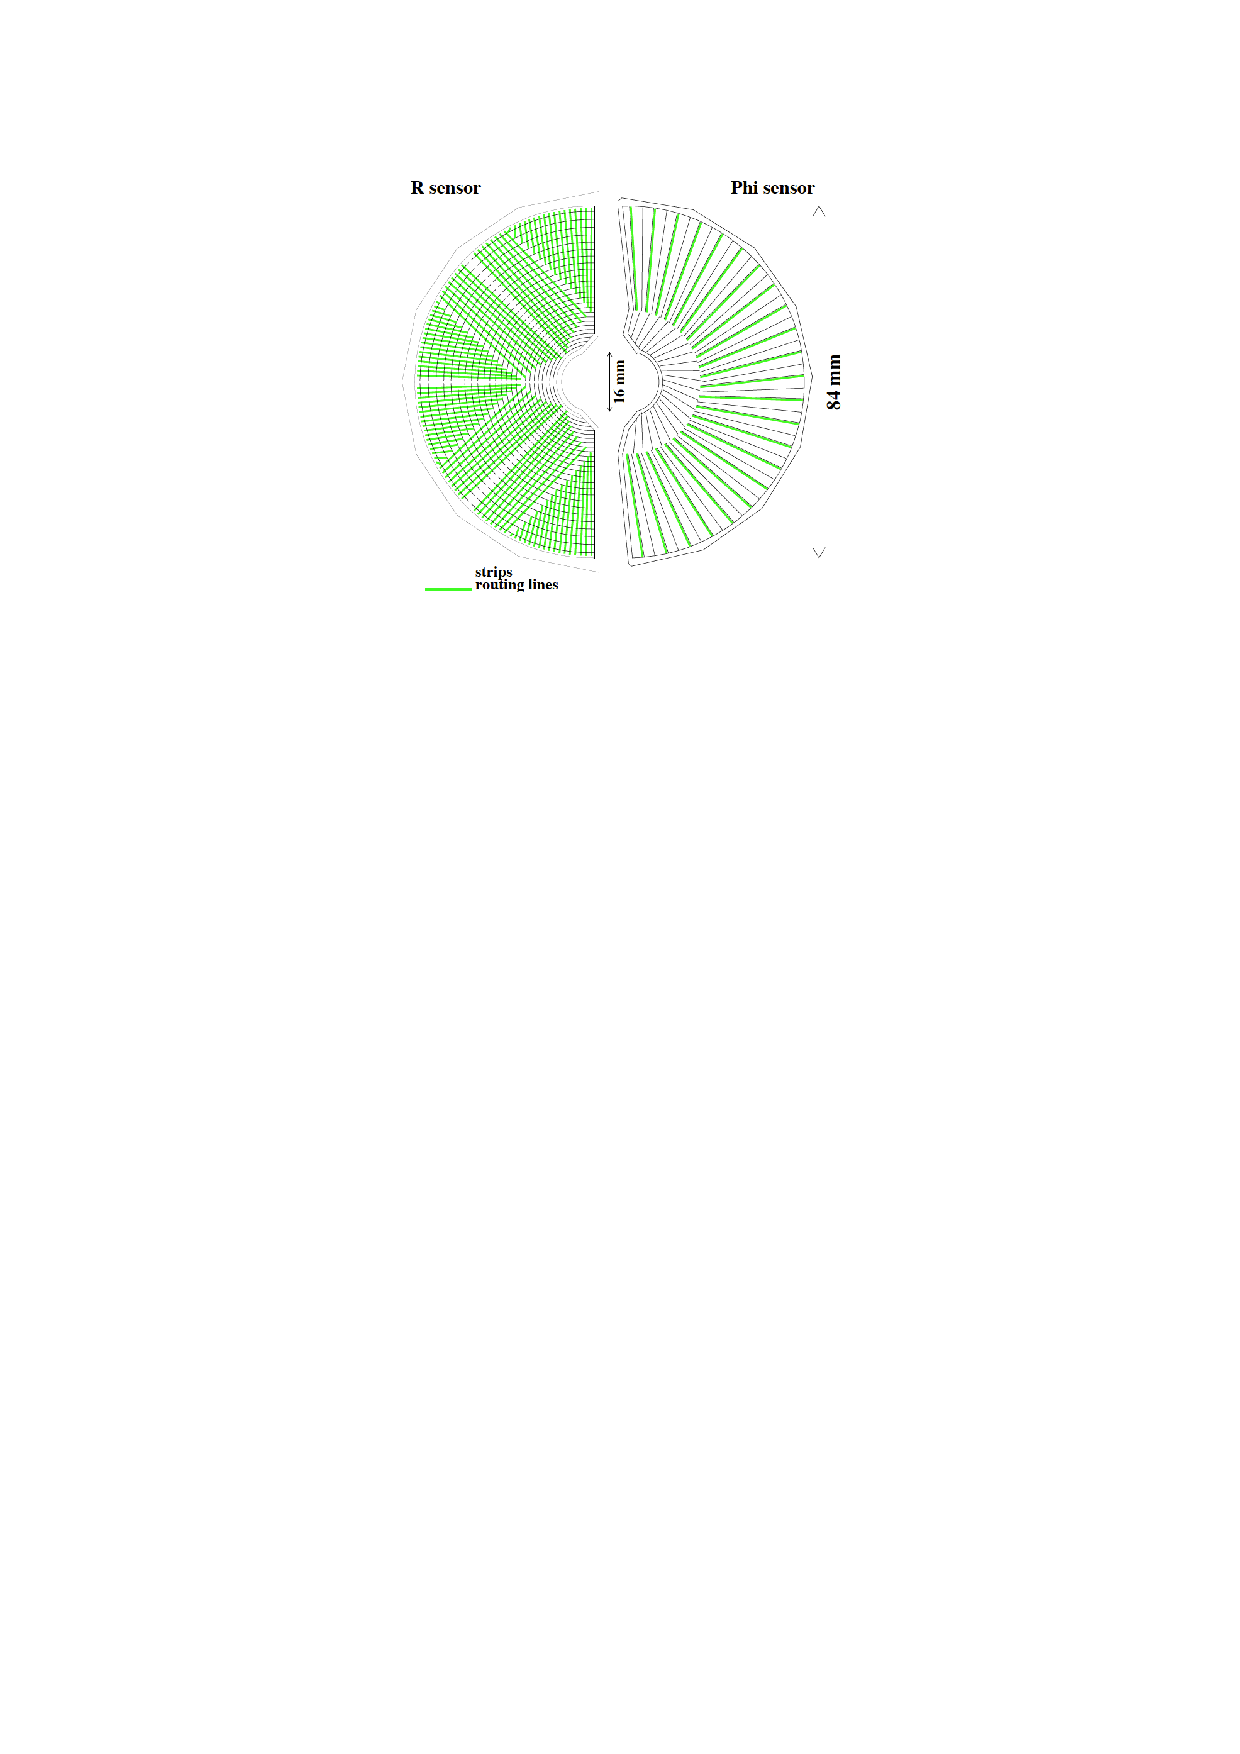
\includegraphics[width=0.4\textwidth]{figs/Detector/velo_r_phi_sensor.pdf}
    \caption{Schematic of an $r$- and $\phi$-sensor in the \velo sub-detector, from Ref.~\cite{LHCb-DP-2014-001}.}
    \label{fig:Dec_r_phi_sensor}   
\end{figure}
%%%%%%%%%%%%%%%%%%%%%%%%%%%%%%%%%%%%%%%%%%%%%%%%%%%%%%%%%%

The sensors are grouped into pairs, called modules. Each of the 21 modules on each side contains sensors for measuring the radial and azimuthal coordinates of the tracks, referred to as $r$- and $\phi$-sensors respectively. A schematic of the two sensor types is shown in Fig.~\ref{fig:Dec_r_phi_sensor}, illustrating the silicon strips and readout channels. 


The \velo modules are arranged to ensure coverage of particles emerging in forward region at angles of 15--300\mrad. The arrangement allows tracks within this acceptance to interact in at least three sensors as shown in Fig.~\ref{fig:Dec_velo_sensor_layout}.   
The modules extend both forward and backwards of the interaction region. Although momentum measurements are not possible for backward tracks, the vertexing of the primary interaction can benefit from this extra information. In the far backward region there are two additional modules, measuring only the radial coordinate. These help to identify pile-up events in which there is more than one primary vertex. 

%%%%%%%%%%%%%%%%%%%%%%%%%%%%%%%%%%%%%%%%%%%%%%%%%%%%%%%%%%
\begin{figure}[!h]
    \centering
    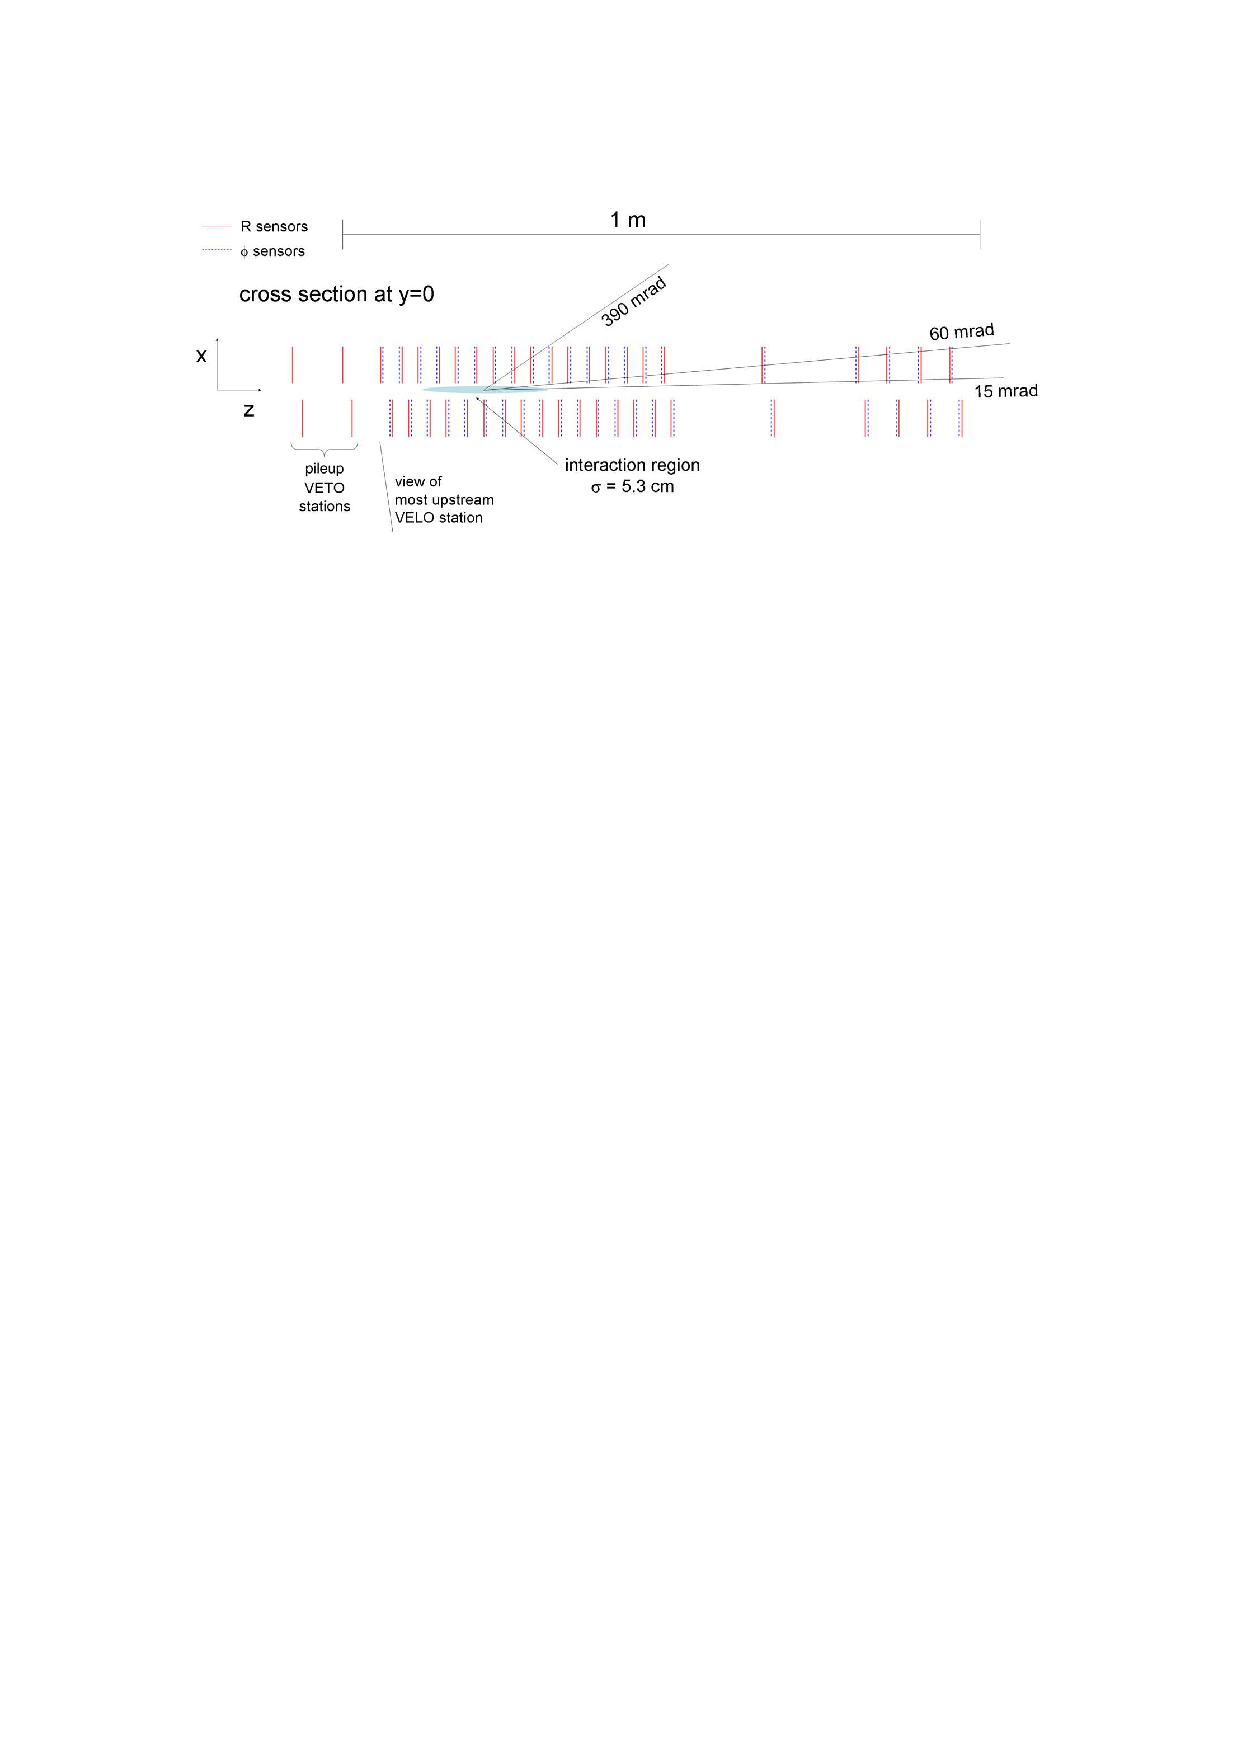
\includegraphics[width=0.8\textwidth]{figs/Detector/velo_sensor_layout.pdf}
    \caption{Schematic of the sensor layout in the \velo sub-detector, from Ref.~\cite{LHCb-DP-2014-001}.}
    \label{fig:Dec_velo_sensor_layout}   
\end{figure}
%%%%%%%%%%%%%%%%%%%%%%%%%%%%%%%%%%%%%%%%%%%%%%%%%%%%%%%%%%

The \velo sub-detector is constructed to operate in the unique environment close to the \lhc beams.

\begin{description}   
\item \textbf{Radiation resistance:} the \velo modules are subjected to extreme and varying amounts of radiation. The detector is designed to with stand three years of nominal \lhc running, using a radiation tolerant semiconductor construction. Additionally, the \velo modules are cooled to remove the heat created from the interactions. The sensors are maintained at a temperature between -10 and 0\degrees\,C with 24\,W of heat removed from each sensor.  
\item \textbf{Radio-frequency (RF) pick-up protection:} the electromagnetic fields generated by the \lhc beams could cause interference in the \velo detectors electronics. Therefore, a shield is used between the modules and the beam-pipe referred to as the RF-foil. This 0.3\mm thick foil separates the \velo and beam-pipe vacuums, providing additional protection to the conditions of the beams from the detector.
\end{description}   

The hits arising from particle interactions in the \velo sensors are extracted from the readout channels using custom analogue \beetle chips. The signals are digitised and combined into clusters in \tell1 readout boards~\cite{HAEFELI2006494}, 


{\color{Red}
\begin{itemize}
\item velo read out chain
\item performance in run1 and run2: track finding efficiency 
\end{itemize}
}




\subsection{Silicon Tracker}

In addition to the \velo, there are two more sub-detectors that utilise silicon sensors in order to determine tracking information. These are collectively referred to at the Silicon Tracker (\st), which is made up of two trackers; the Tracker Turicensis (\ttracker) and Inner Tracker (\intr). The \ttracker is located before the dipole magnet, whereas the \intr is positioned after, as show in Fig.~\ref{fig:Dec_lhcb_Schematic}. Although these two detectors are spatially separated, their common silicon mircostrip sensors and electronics warrant considering them together.

The silicon sensors are made up of single-sided $p^{+}$-on-$n$ sensors. The hits are read out via chips at the end of each module. These chips are the same custom analogue \beetle chips used in the \velo. The signals pass to into digitisers and then through optical fibres into \tell1 boards that perform clustering algorithms.
Both sub-detectors are cooled to 5\degrees{C} and their sealed containers flushed with nitrogen gas to prevent condensation.


{\color{Red}
\begin{itemize}
\item performance
\end{itemize}
}


\subsubsection{Tracker Turicensis}

The \ttracker is positioned before the dipole magnet and covers the entire \lhcb acceptance, standing 130\cm tall and 150\cm wide.
It is made up of four layers orientated at angles to one another. The first and fourth layers are parallel, with the second and third at angles -5\degrees and +5\degrees to these respectively. The first and second are separated from the third and fourth by 27\cm along the beam axis. The layout of the silicon modules in the \ttracker is shown in Fig.~\ref{fig:Dec_tt_layout}. The sensors are grouped into \emph{half-modules} that span half of the vertical height of the sub-detector. These are made up of seven silicon sensors and a readout hybrid at the outermost end. The readout electronics are positioned outside of the \lhcb acceptance, limiting the amount of multiple scattering due to interactions with the detector material. 

%%%%%%%%%%%%%%%%%%%%%%%%%%%%%%%%%%%%%%%%%%%%%%%%%%%%%%%%%%
\begin{figure}[!h]
    \centering
    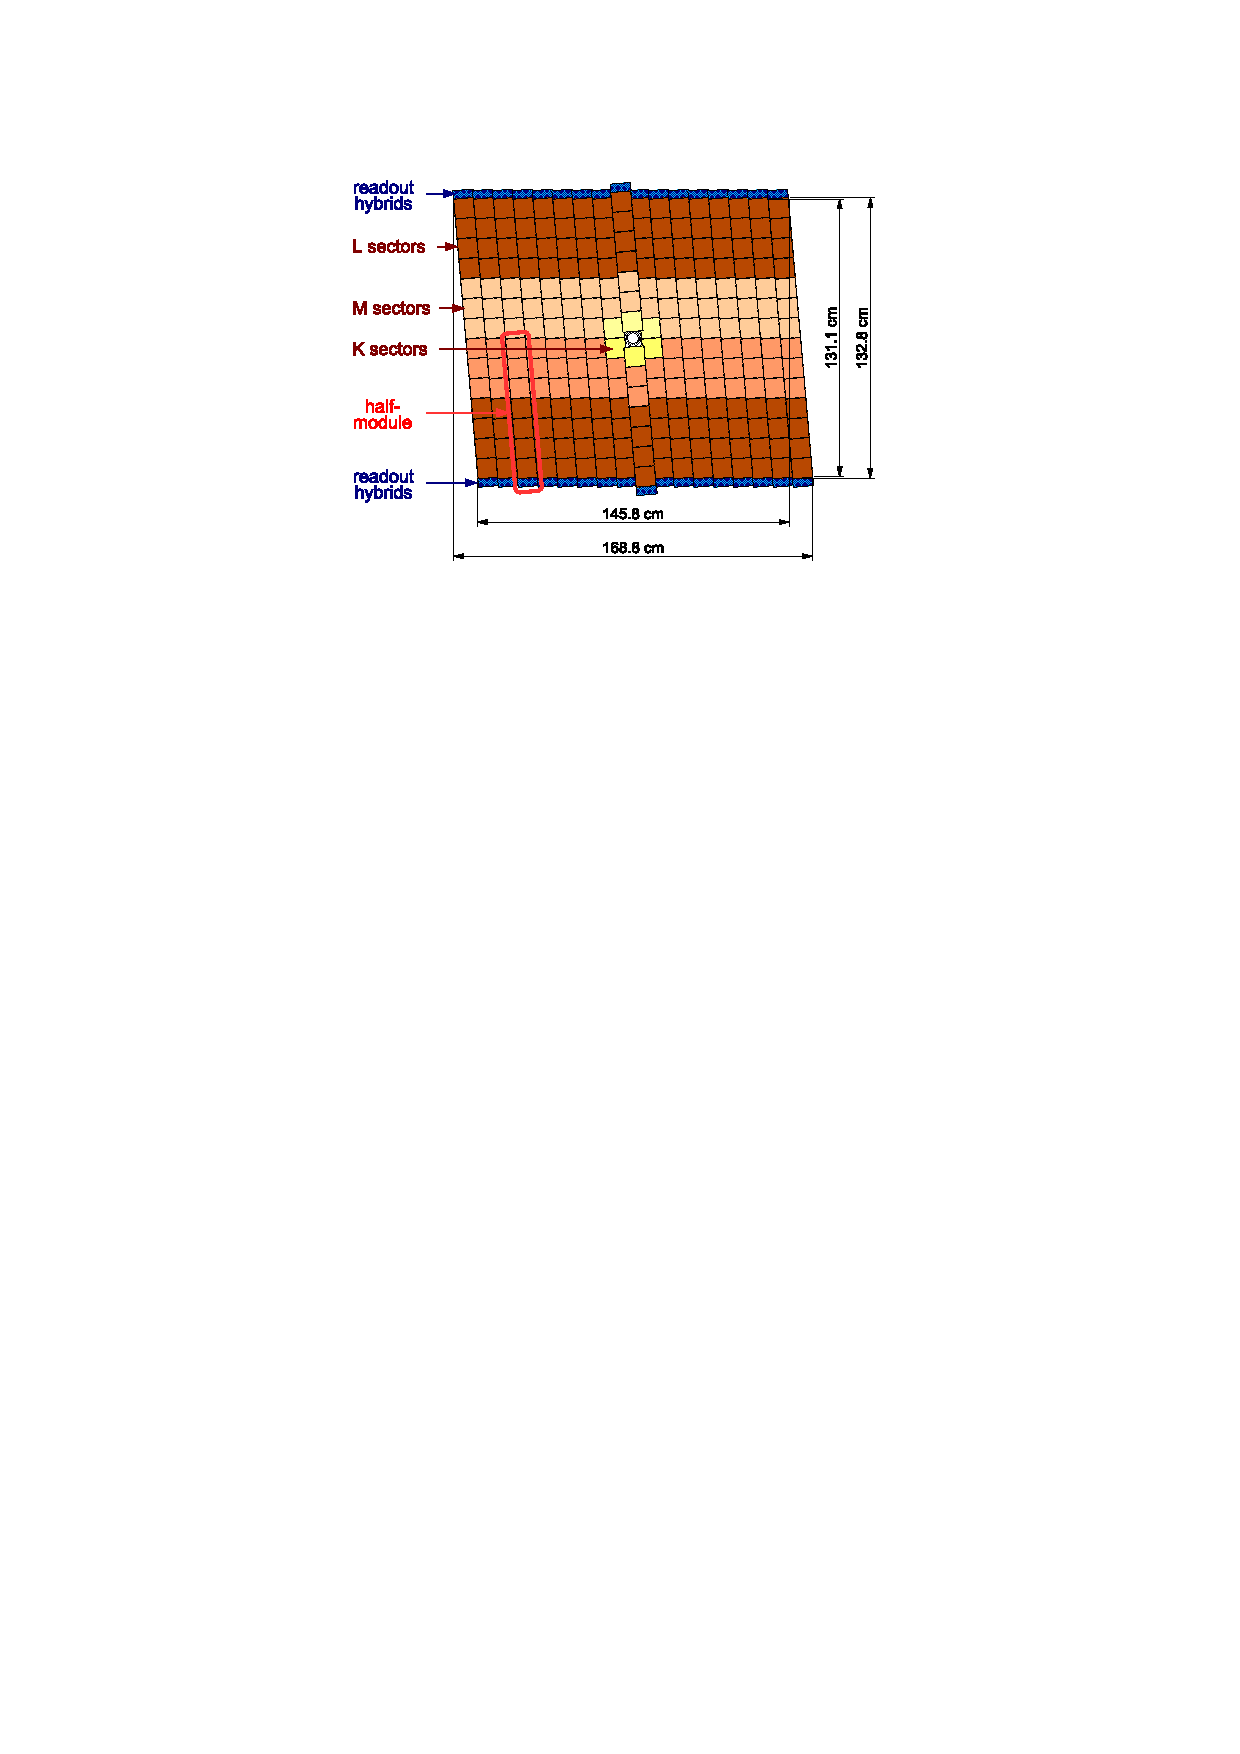
\includegraphics[width=0.6\textwidth]{figs/Detector/tt_layout.pdf}
    \caption{Schematic of the \ttracker sub-detector, from Ref.~\cite{Alves:2008zz}.}
    \label{fig:Dec_tt_layout}   
\end{figure}
%%%%%%%%%%%%%%%%%%%%%%%%%%%%%%%%%%%%%%%%%%%%%%%%%%%%%%%%%%

The \emph{half-modules} are arranged to prevent any gaps in the instrumentation. The adjacent \emph{half-modules} are offset by 1\cm along the beam axis, allowing the modules to overlap by a few millimetres in the $x$-axis. 


{\color{Red}
\begin{itemize}
\item performance
\end{itemize}
}


\subsubsection{Inner Tracker}

The \intr is the second silicon detector making up the \st. It is located after the dipole magnet in three tracking stations. As the name implies, it covers only the inner region of the acceptance, measuring 140\cm wide and 40\cm tall. The rest of the area is covered by the much larger Outer Tracker. Similar to the \ttracker, the \intr is made up of four layers positioned at slight angles to one another. However, as shown in Fig.~\ref{fig:Dec_lhcb_Schematic}, there are three separate \intr stations, each containing four layers.
These stations are constructed as of four boxes distributed around the beam-pipe in a cross shape, as shown in Fig.~\ref{fig:Dec_it_layout}. 

%%%%%%%%%%%%%%%%%%%%%%%%%%%%%%%%%%%%%%%%%%%%%%%%%%%%%%%%%%
\begin{figure}[!h]
    \centering
    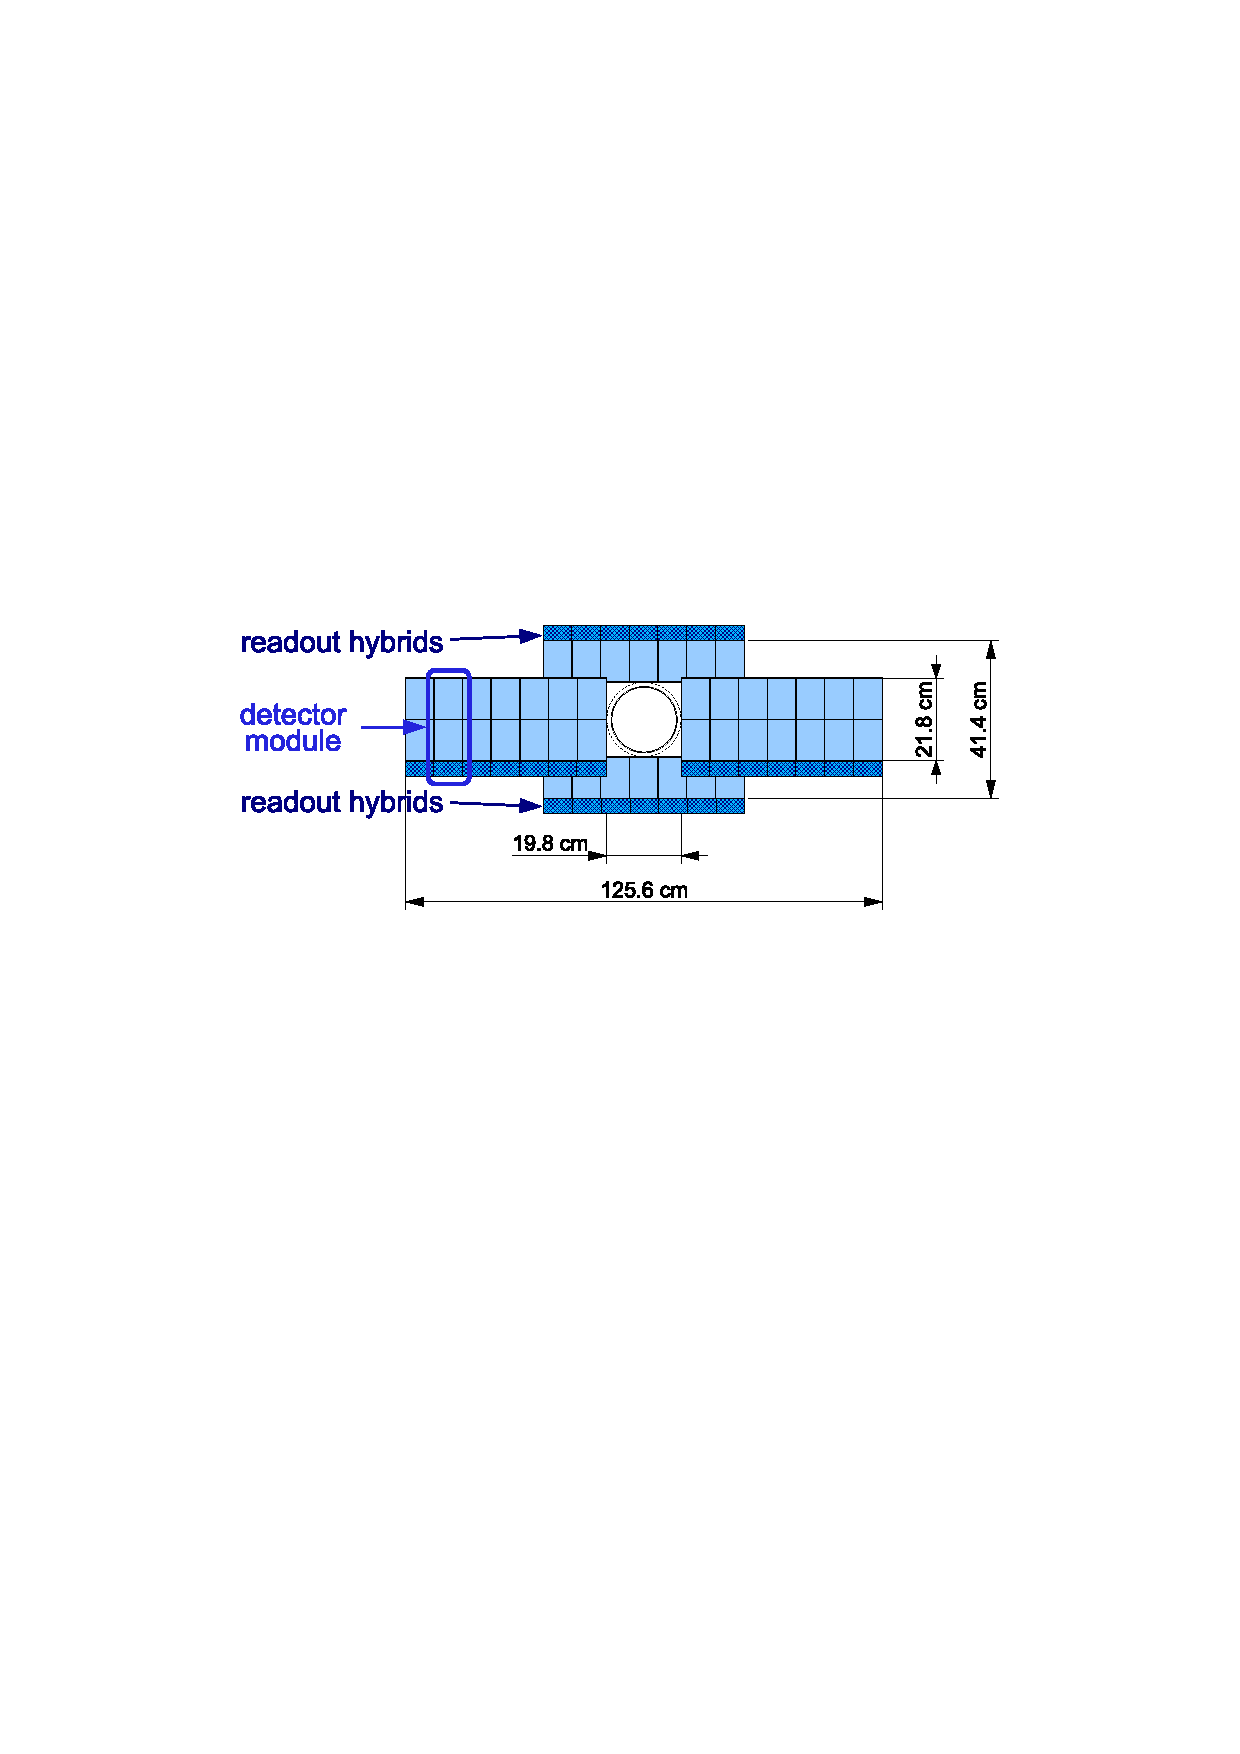
\includegraphics[width=0.6\textwidth]{figs/Detector/it_layout.pdf}
    \caption{Schematic of the \intr sub-detector, from Ref.~\cite{Alves:2008zz}.}
    \label{fig:Dec_it_layout}   
\end{figure}
%%%%%%%%%%%%%%%%%%%%%%%%%%%%%%%%%%%%%%%%%%%%%%%%%%%%%%%%%%

The detector modules consist of either one or two silicon sensors and a readout chip. These are also offset along the beam axis to allow the modules to overlap slightly in the $x$-axis.



\subsection{Outer Tracker}

In contrast to the the silicon-based sub-detectors already described, the Outer Tracker (\ot) is a straw tube tracker filled with a gaseous mixture of argon, carbon dioxide and oxygen. The 4.9\mm diameter straws are 2.4\m in length and arranged in double layers as shown in Fig.~\ref{fig:Dec_ot_schematic}. As with the \intr, the \ot is split into three stations. Each of these stations similarly has four layers arranged at angles to one another $(0\degrees,-5\degrees,+5\degrees,0\degrees)$. The arrangement of the stations and layers are also shown in Fig.~\ref{fig:Dec_ot_schematic}. The inner region occupied by the \intr is visible.
 
%%%%%%%%%%%%%%%%%%%%%%%%%%%%%%%%%%%%%%%%%%%%%%%%%%%%%%%%%%
\begin{figure}[!h]
    \centering
    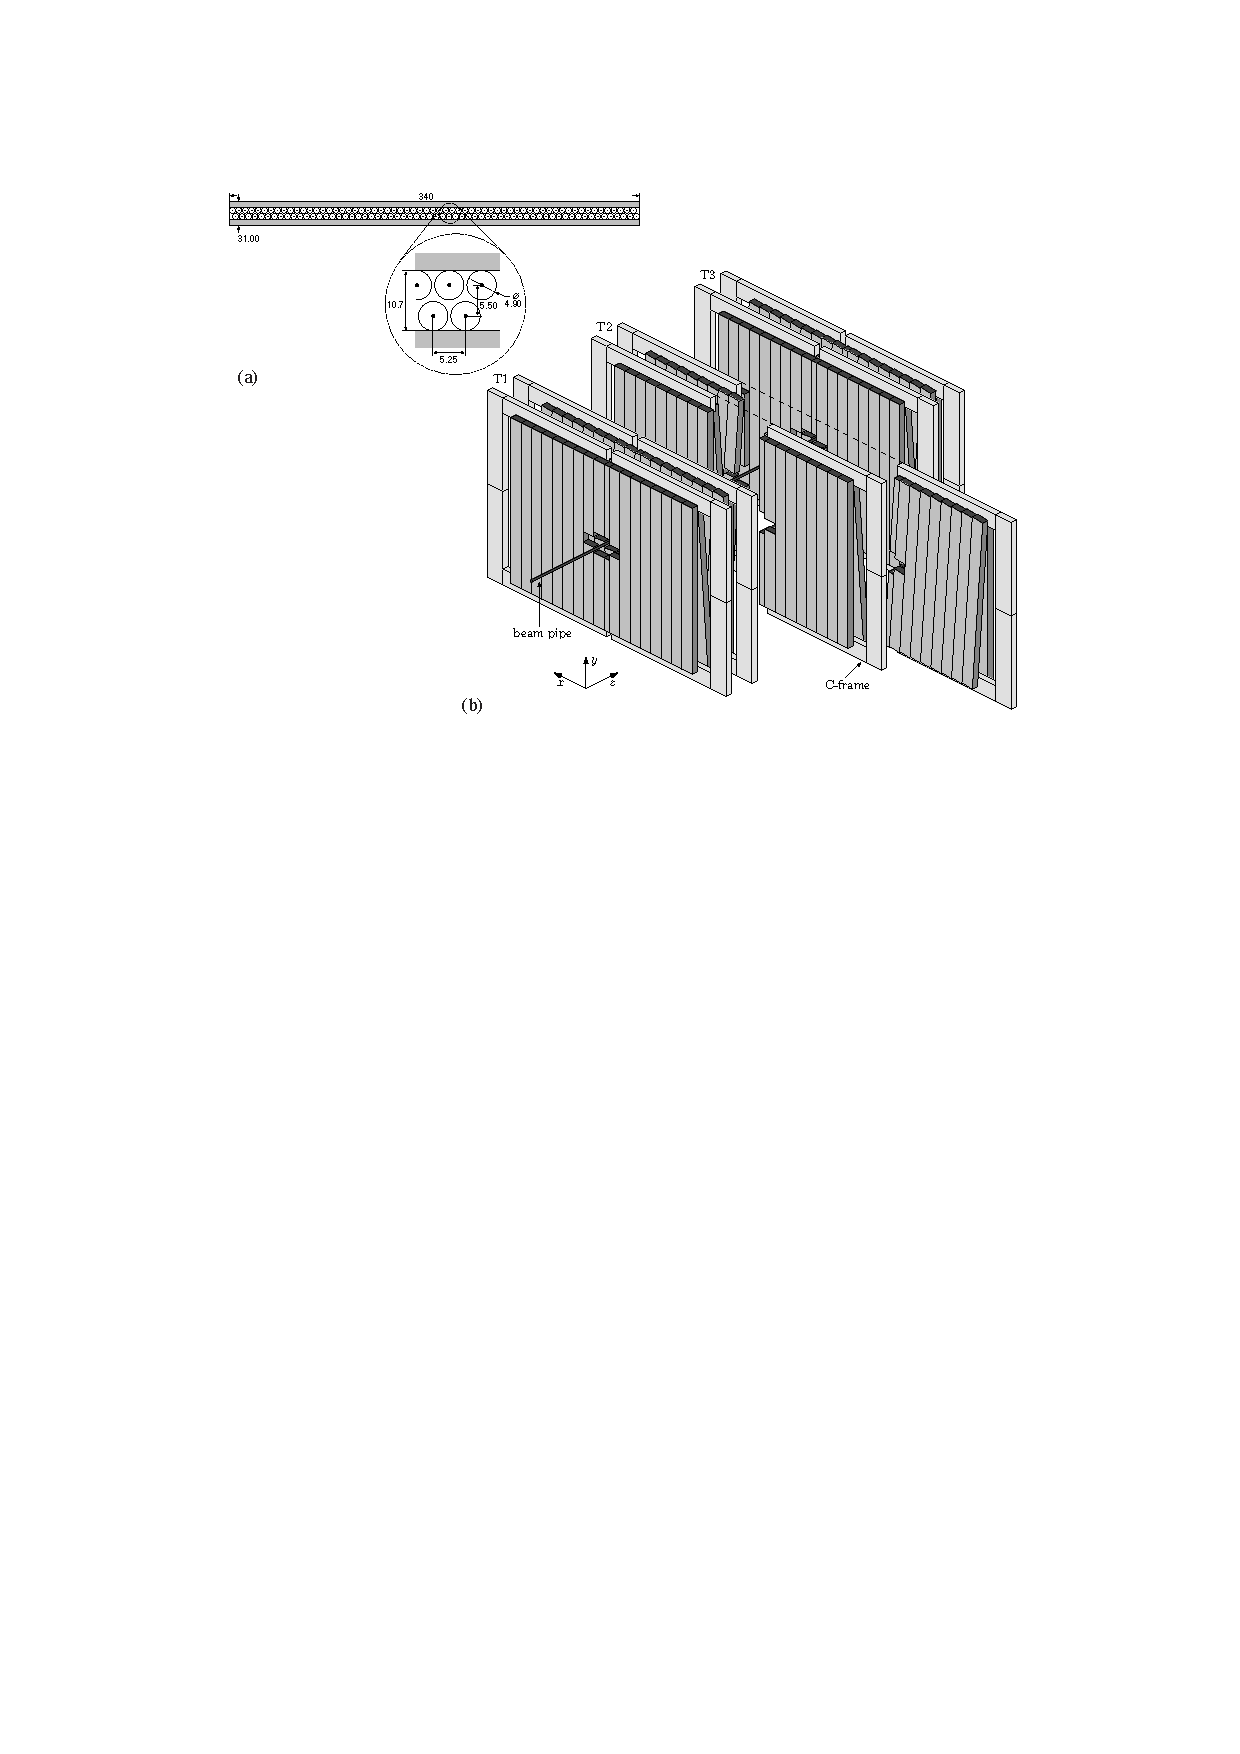
\includegraphics[width=0.8\textwidth]{figs/Detector/ot_layout.pdf}
    \caption{Schematic of the \ot sub-detector, from Ref.~\cite{LHCb-DP-2013-003}.}
    \label{fig:Dec_ot_schematic}   
\end{figure}
%%%%%%%%%%%%%%%%%%%%%%%%%%%%%%%%%%%%%%%%%%%%%%%%%%%%%%%%%%



\subsection{Ring imaging Cherenkov detectors}

The ring imaging Cherenkov detectors (\rich) provide essential information about the particle identification of tracks, allowing different species to be distinguished. This means that kaons and protons can be distinguished from the abundant pions tracks in a typical event. Two \rich sub-detectors are present, each optimised for particles with different momentums. The first, \richone, is located between the \velo and \ttracker, before the particles have passed through the magnetic field. This provides discrimination primarily for low momentum tracks between 1--60\gevc. A second sub-detector, \richtwo, is located between the \intr and \ot tracking stations and calorimeters, after the particles have travelled through the magnetic field. This caters for the higher momentum particles in the range 15--100\gevc. 


{\color{Red}
\begin{itemize}
\item rich principle 
\item mirrors
\item HPDs
\item pattern recognition 
\end{itemize}
}

%%%%%%%%%%%%%%%%%%%%%%%%%%%%%%%%%%%%%%%%%%%%%%%%%%%%%%%%%%
\begin{figure}[!h]
    \centering
    \begin{subfigure}[t]{0.4\textwidth}
        \centering        
        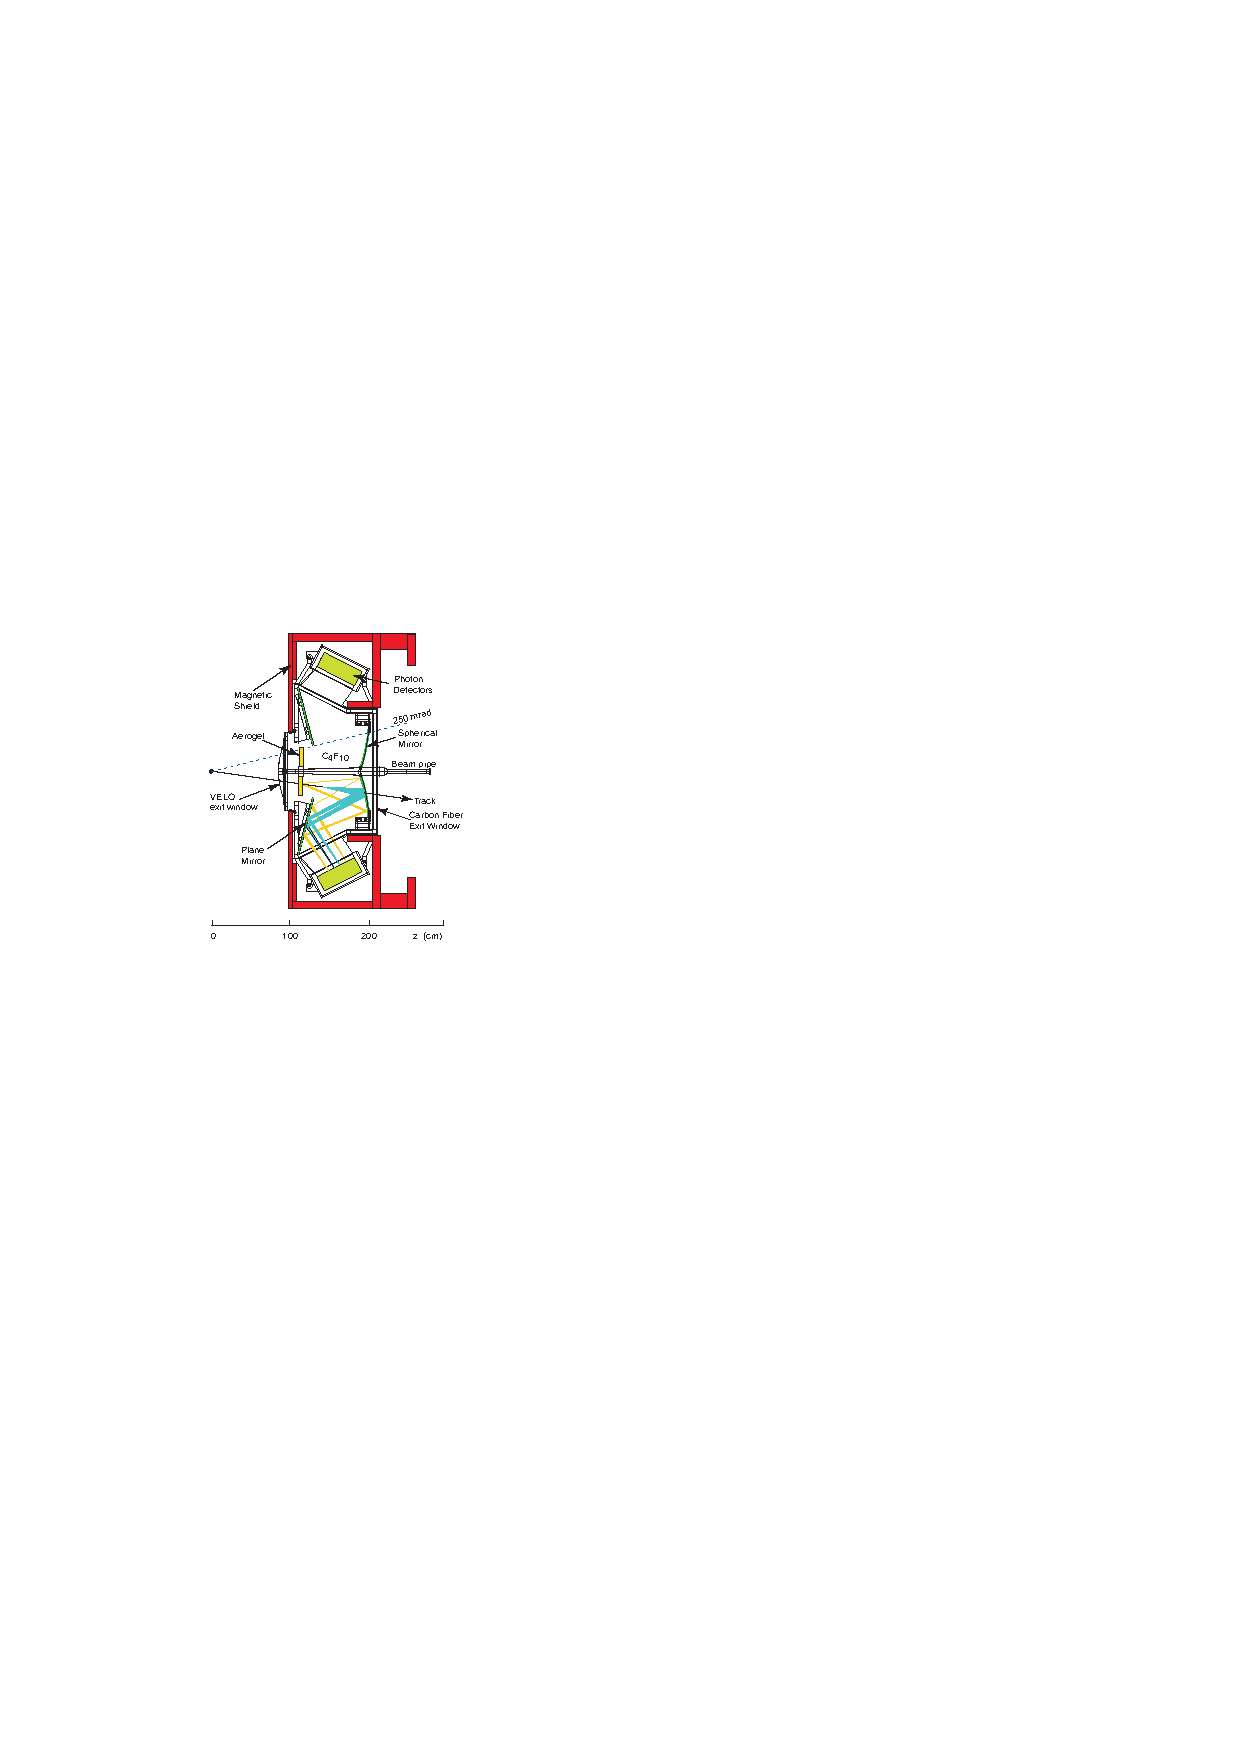
\includegraphics[width=1.0\textwidth]{figs/Detector/richone_layout.pdf}
        \caption{\richone}
    \end{subfigure}
    \begin{subfigure}[t]{0.4\textwidth}
        \centering
        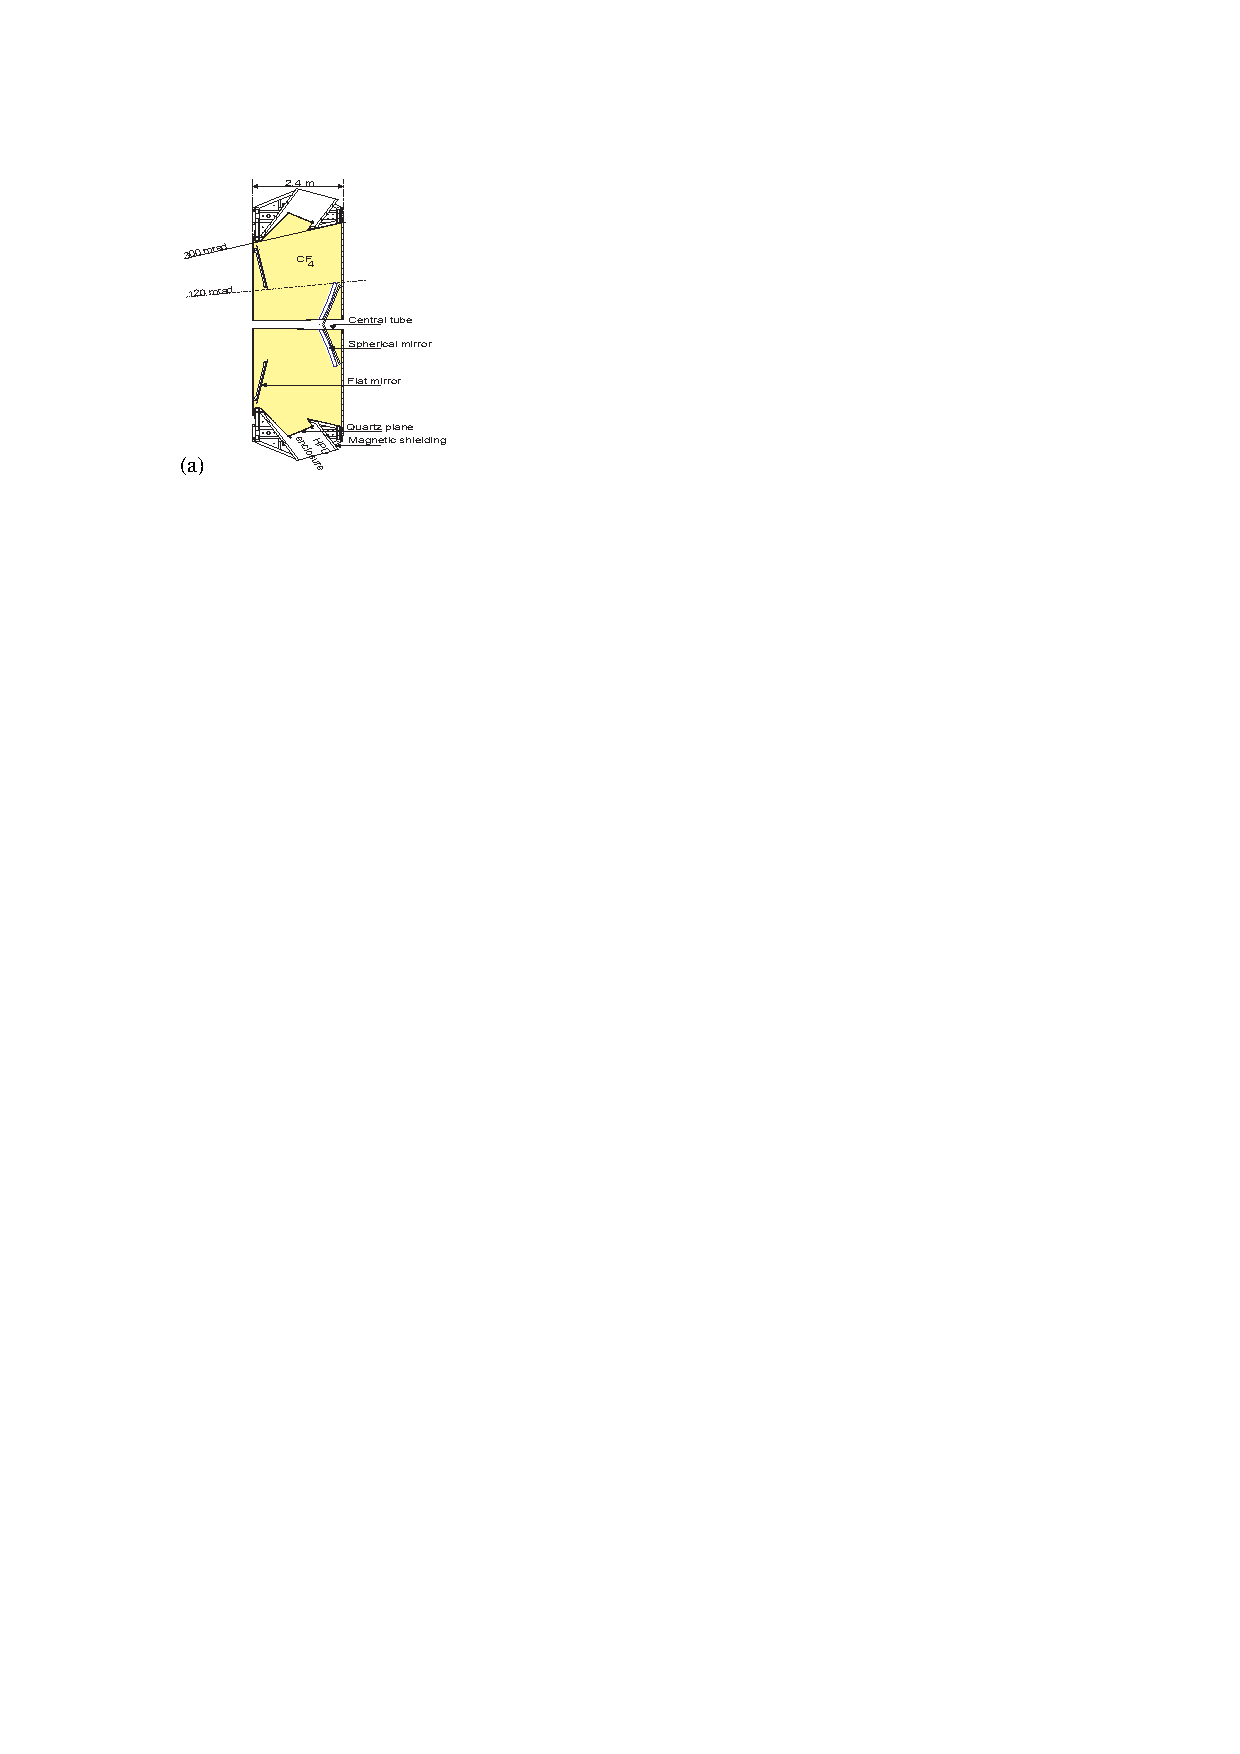
\includegraphics[width=1.0\textwidth]{figs/Detector/richtwo_layout.pdf}
        \caption{\richtwo}
    \end{subfigure}
    \caption{Schematic the \richone and \richtwo sub-detectors from Ref.~\cite{Alves:2008zz}.}

    \label{fig:Dec_rich_layout}   
\end{figure}
%%%%%%%%%%%%%%%%%%%%%%%%%%%%%%%%%%%%%%%%%%%%%%%%%%%%%%%%%%

\subsubsection{\richone}

{\color{Red}
\begin{itemize}
\item radiator and refractive indices 
\item talk about aero gel being removed
\item find some references 
\end{itemize}
}

\subsubsection{\richtwo}

{\color{Red}
\begin{itemize}
\item radiator and refractive indices 
\end{itemize}
}

\subsection{Calorimeters}

The calorimeters measure the energy deposited by particles. This is crucial for the reconstruction of neutral particles that don't leave tracks in the tracking stations. Additionally, the calorimeter plays an important role in the triggering of events.

\subsubsection{Pre-shower detector}
\subsubsection{Electronic Calorimeter}
\subsubsection{Hadron calorimeter}

\subsection{Muon system}

%%%%%%%%%%%%%%%%%%%%%%%%%%%%%%%%%%%%%%%%%%%%%%%%%%%%%%%%%%
\begin{figure}[!h]
    \centering
    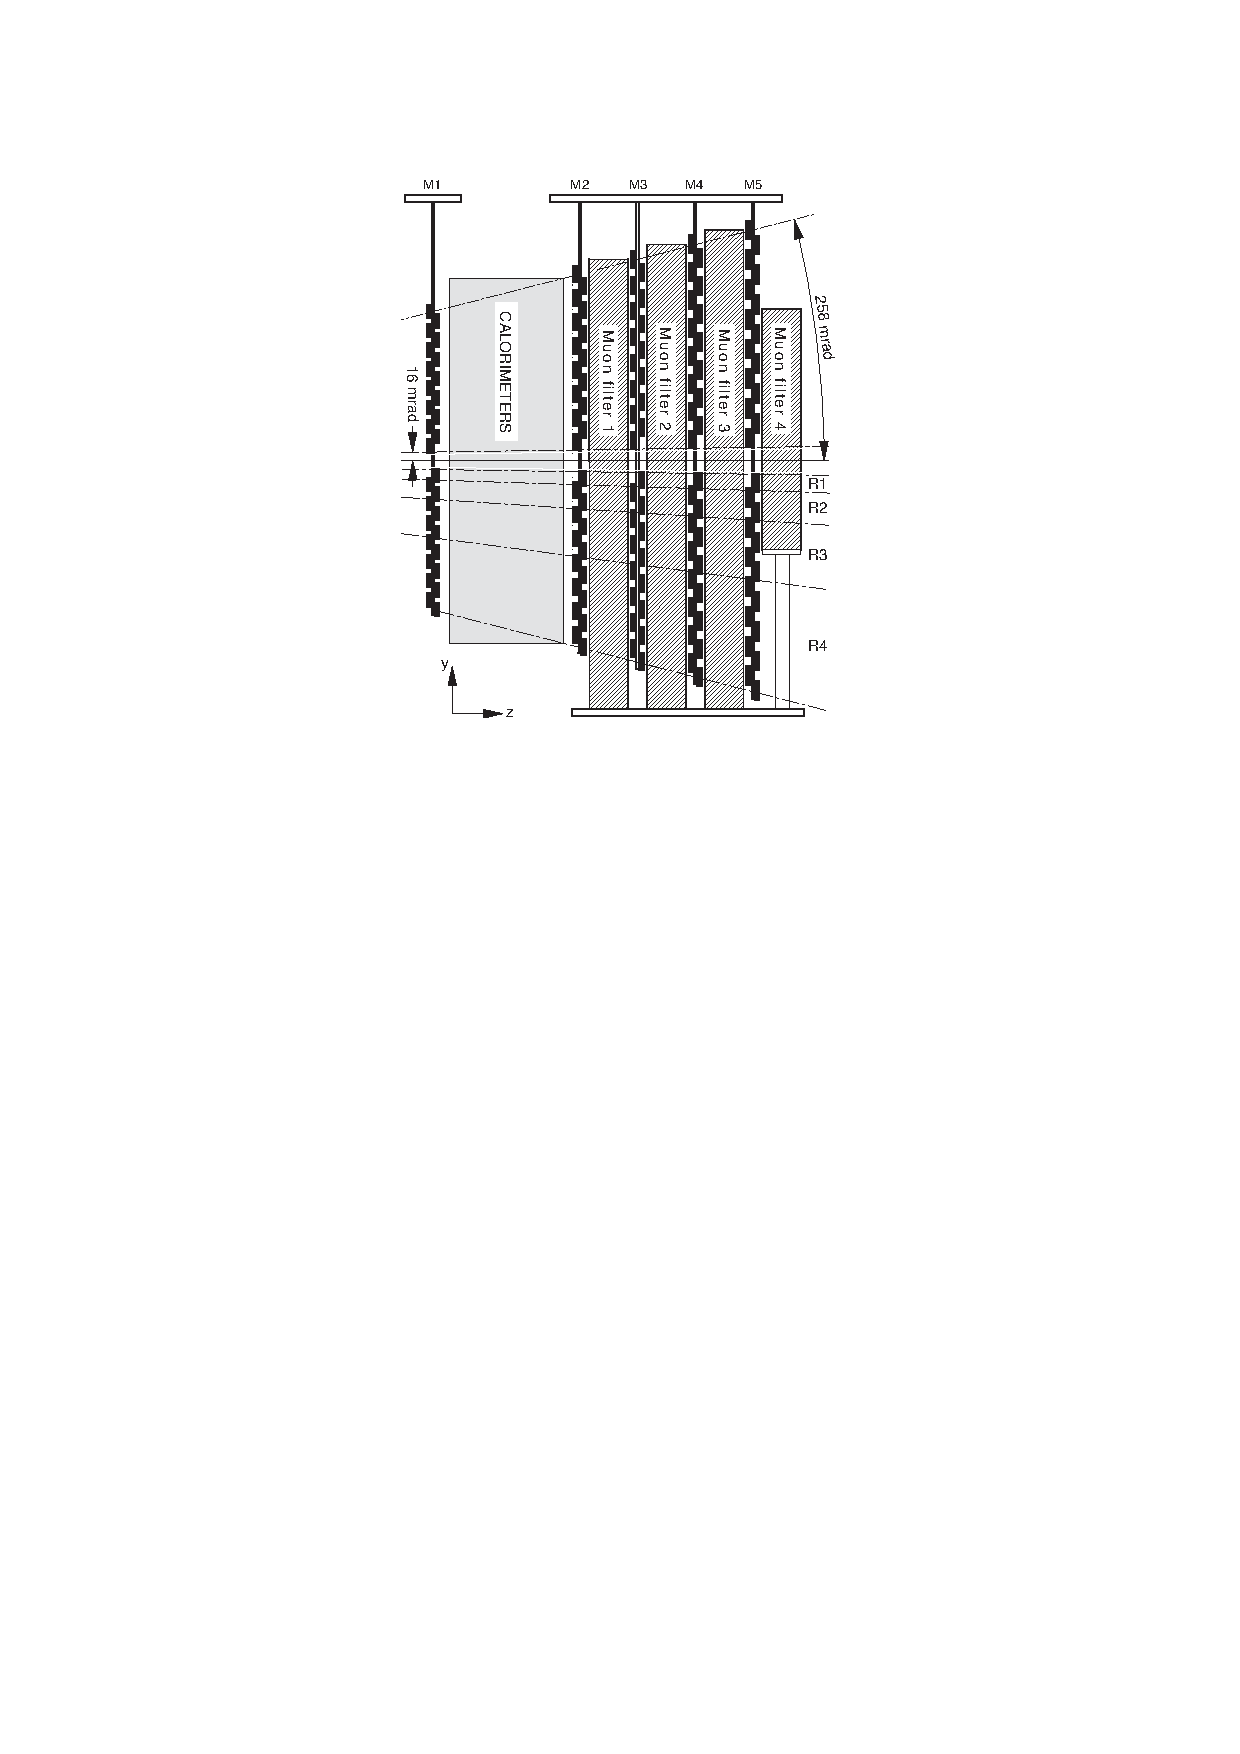
\includegraphics[width=0.4\textwidth]{figs/Detector/muon_layout.pdf}
    \caption{Schematic of the Muon sub-detector, from Ref.~\cite{Alves:2008zz}.}
    \label{fig:Dec_muon_schematic}   
\end{figure}
%%%%%%%%%%%%%%%%%%%%%%%%%%%%%%%%%%%%%%%%%%%%%%%%%%%%%%%%%%

\subsection{Trigger}
\subsubsection{\lone}
\subsubsection{\hltone}
\subsubsection{\hlttwo}

\subsection{Reconstruction}
\subsubsection{Track Reconstruction}


%%%%%%%%%%%%%%%%%%%%%%%%%%%%%%%%%%%%%%%%%%%%%%%%%%%%%%%%%%
\begin{figure}[!h]
    \centering
    \begin{subfigure}[t]{0.4\textwidth}
        \centering
        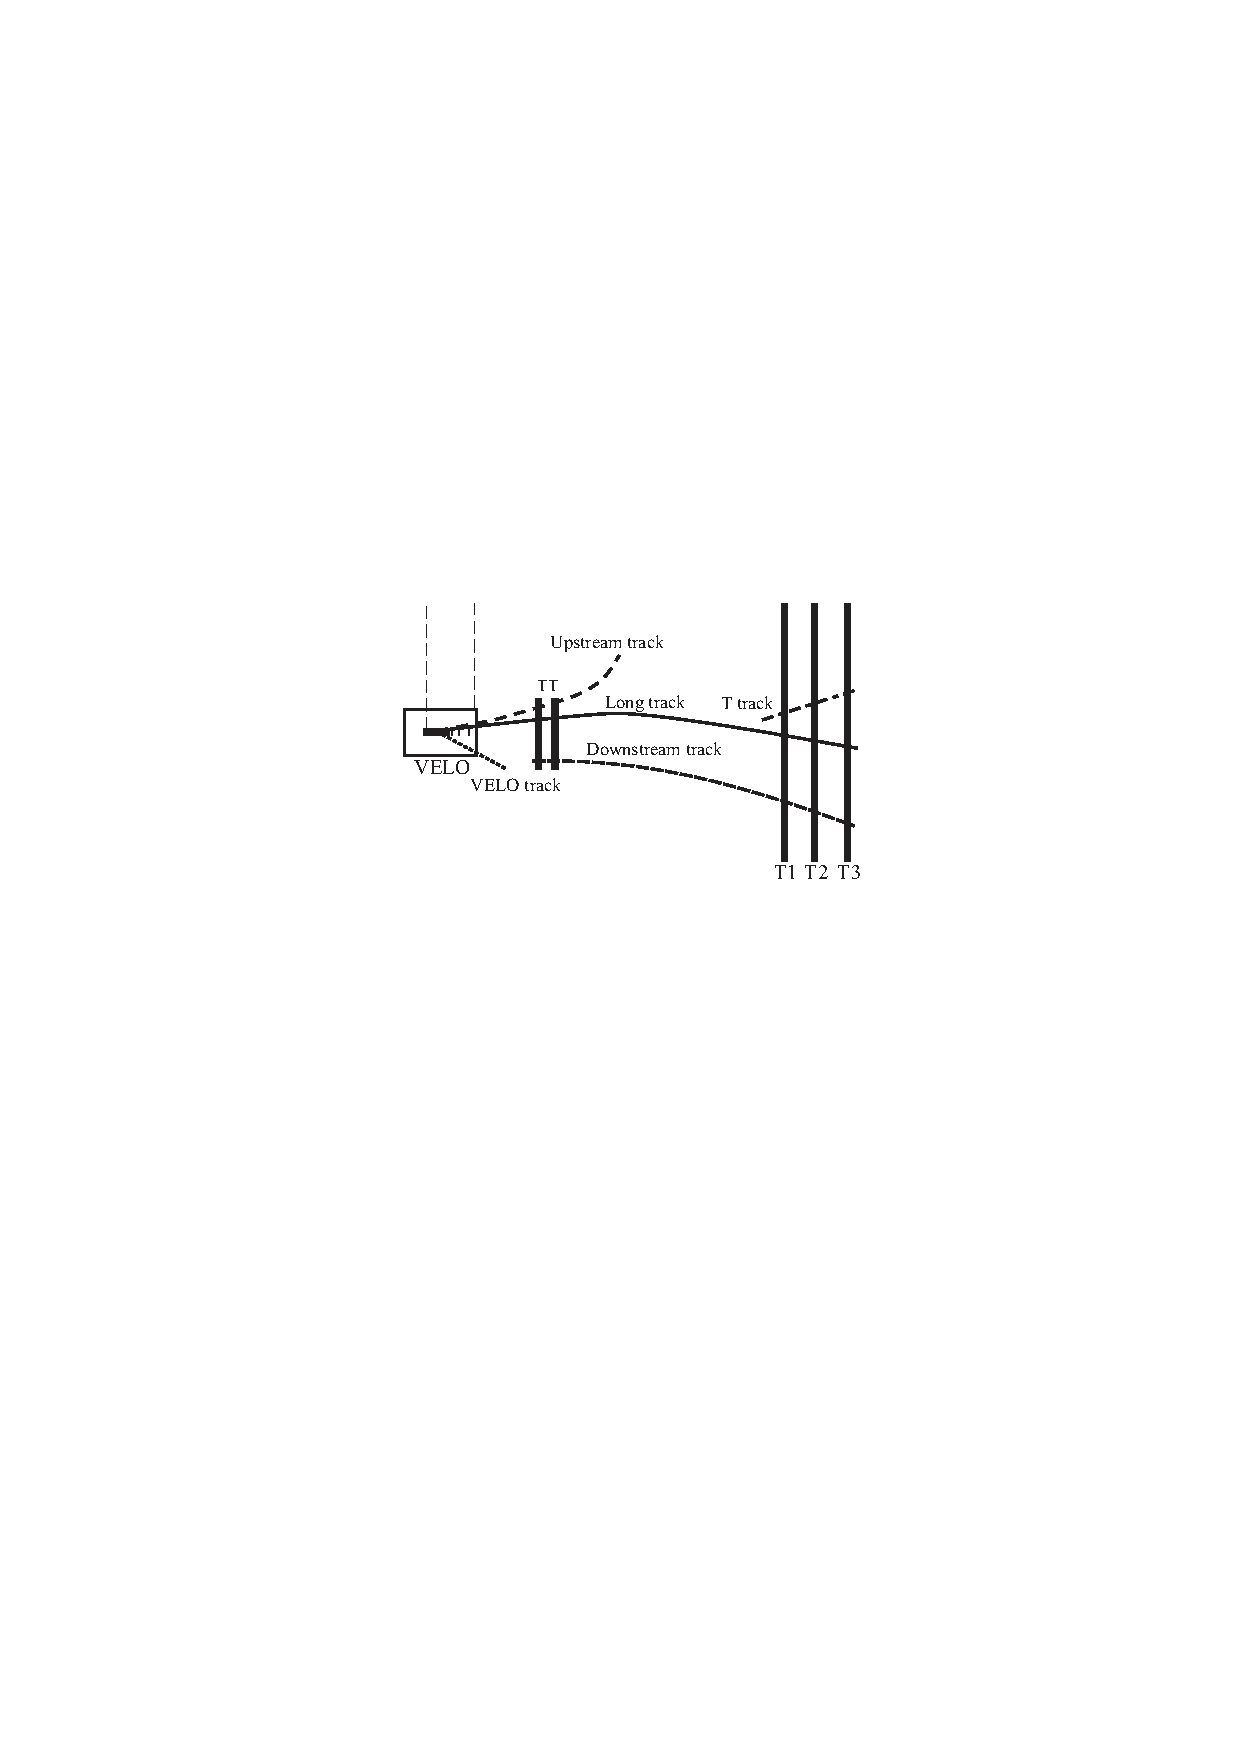
\includegraphics[width=1.0\textwidth]{figs/Detector/reco_track_types.pdf}
    \end{subfigure}
    \begin{subfigure}[t]{0.4\textwidth}
        \centering
        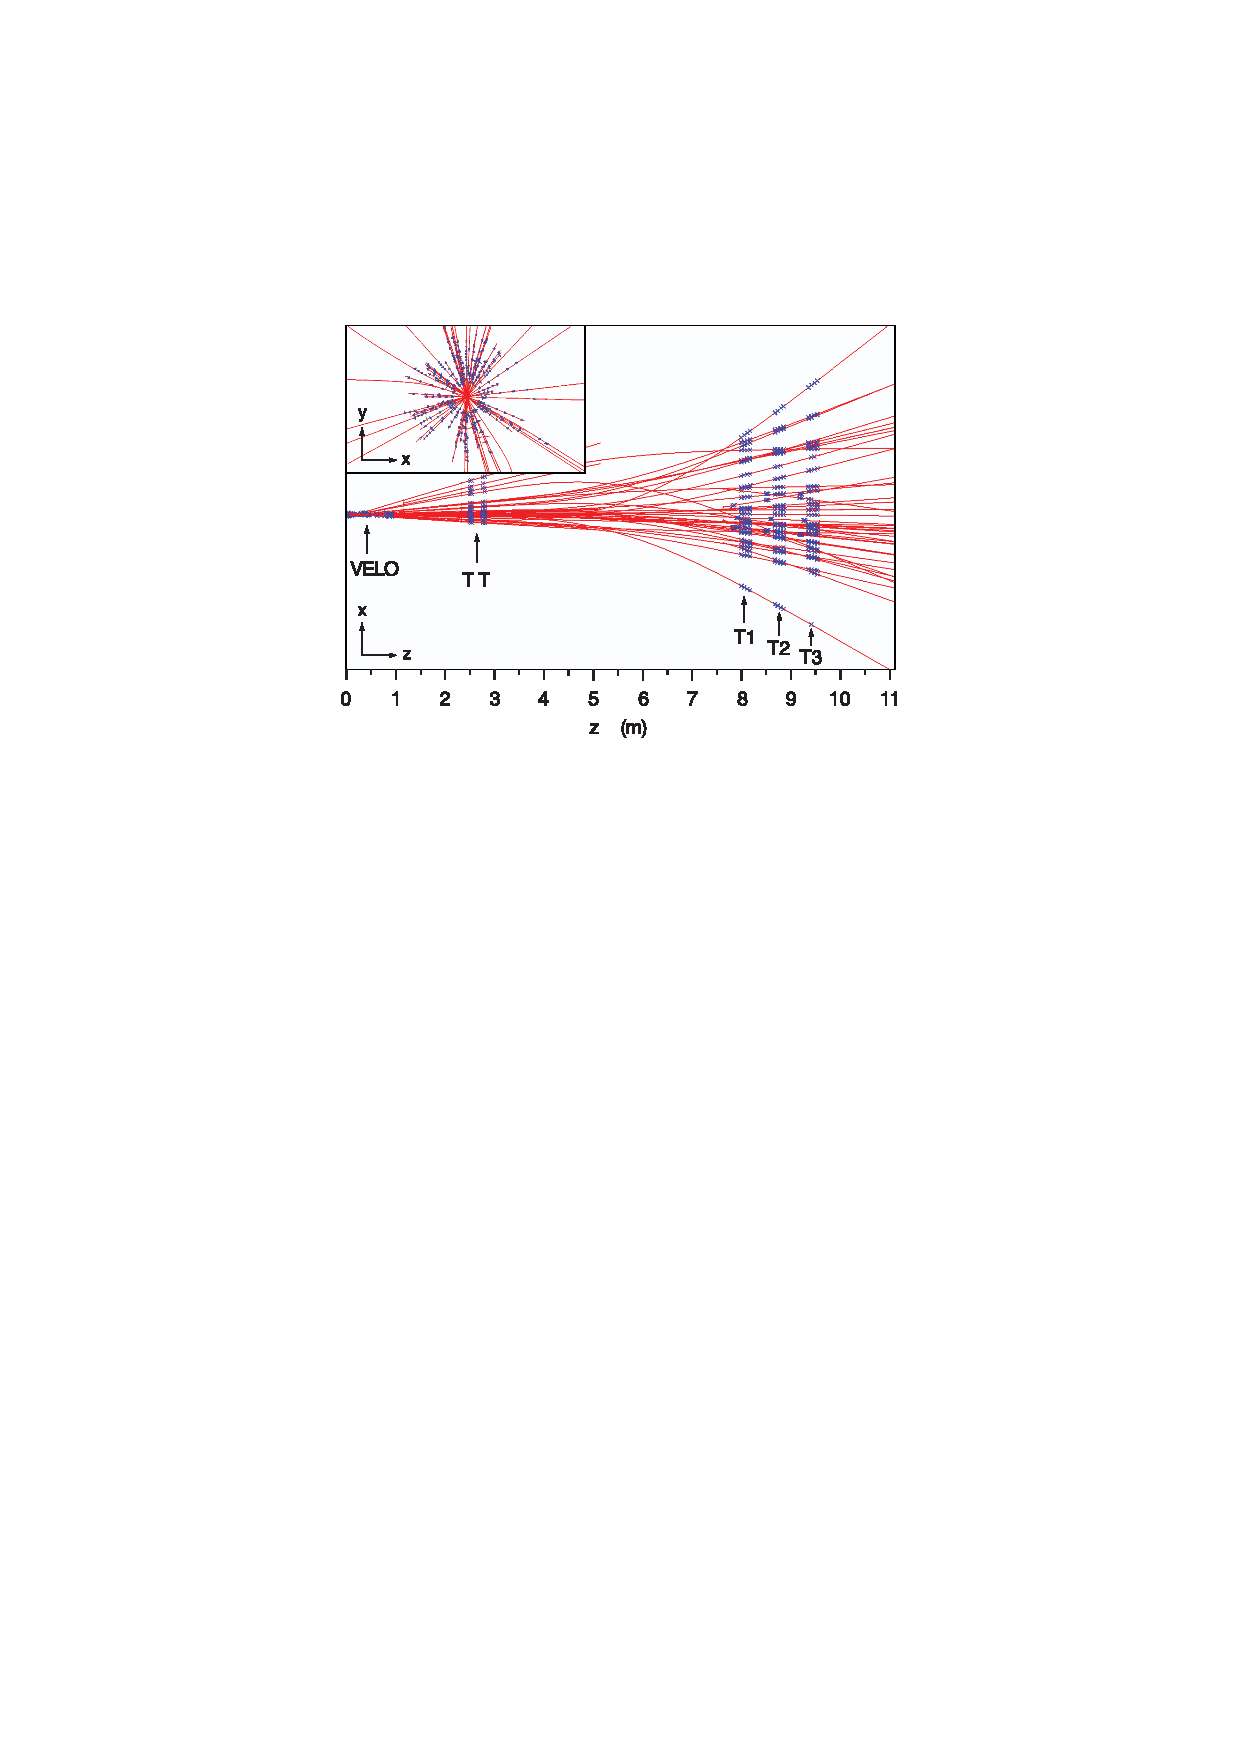
\includegraphics[width=1.0\textwidth]{figs/Detector/reco_track_reco.pdf}
    \end{subfigure}
    \caption{Diagram of the different track reconstruction types (left) and an illustration of the reconstructed tracks in a typical event from Ref.~\cite{LHCb-DP-2014-002}.}
    \label{fig:Dec_reco_tracks}   
\end{figure}
%%%%%%%%%%%%%%%%%%%%%%%%%%%%%%%%%%%%%%%%%%%%%%%%%%%%%%%%%%

\section{VELO resolution and luminosity determination}
\chapter{Event selection} 
\label{ch:selection}

\minitoc

In this chapter the procedures developed to reconstruct and select \decay{\Bp}{\Dsp\phiz} and \decay{\Bp}{\Dsp\Kp\Km} candidates are described. 
In both cases the branching fractions are measured relative to the normalisation channel \decay{\Bp}{\Dsp\Dzb}.
The corresponding selection for the normalisation channel \decay{\Bp}{\Dsp\Dzb} is also described.  


\section{Data samples and Simulations}



\subsection{Data samples}
\label{sec:data}

The searches for \decay{\Bp}{\Dsp\phiz} and \decay{\Bp}{\Dsp\Kp\Km} decays are performed using a combined data sample comprising of the entire Run I data set and a part of the Run II data set, namely the years 2015 and 2016.
The total integrated luminosity obtained for each year is listed in Table~\ref{tab:lumi}, along with the corresponding centre-of-mass energies. 

\begin{table}[h]
   \centering
      \begin{tabular}{ccc}
         \hline
         Year                    & Integrated luminosity (\invfb)  & $\sqrt{s}$ (\tev) \\ 
         \hline
         2011                    & 1.0  &  7 \\
         2012                    & 2.0  &  8 \\
         2015                    & 0.3  & 13 \\
         2016                    & 1.5  & 13 \\
         \hline
      \end{tabular}
   
   \caption{The integrated luminosities obtained during the different data taking periods used in this analysis and the corresponding centre-of-mass energies ($\sqrt{s}$).}
   \label{tab:lumi}
\end{table}

\subsection{Simulation samples}
\label{sec:mc}

Many aspects of the searches for \decay{\Bp}{\Dsp\phiz} and \decay{\Bp}{\Dsp\Kp\Km} decays requires input from simulation samples. This includes the relative selection efficiencies of the signal and normalisation channels and the determination of the invariant mass distributions of the candidates.
The samples are generated separately for each of the running periods listed in Table~\ref{tab:lumi} and for both polarities of the \lhcb dipole magnet. The simulation samples for \decay{\Bp}{\Dsp\phiz} and \decay{\Bp}{\Dsp\Dzb} decays are generated assuming they proceed via pseudo-two-body decays. In contrast, the phase-space dependence of \decay{\Bp}{\Dsp\Kp\Km} decays must be considered when generating these simulations. Samples are generating assuming a flat distribution across the phase-space. 
Additionally, simulations samples are required for many of the background processes considered in the analyses. These are generated using the same framework and processed using the same reconstruction as the signal modes.


In the simulations, $pp$ collisions are generated using \pythia~\cite{Sjostrand:2007gs,Sjostrand:2006za} with a specific \lhcb configuration~\cite{LHCb-PROC-2010-056}.  Decays of hadronic particles are described by \evtgen~\cite{Lange:2001uf}, in which final-state radiation is generated using \photos~\cite{Golonka:2005pn}. The interaction of the generated particles with the detector, and its response, are implemented using the \geant toolkit~\cite{Allison:2006ve, *Agostinelli:2002hh} as described in Ref.~\cite{LHCb-PROC-2011-006}.


\section{Online selection}
\label{sec:selection_trigger}

The nominal collision frequency at the \lhc is 40\,MHz. In Run II, this corresponded to a peak \Bpm-hadron production rate of around 17\,kHz, assuming a peak luminosity of $\mathcal{L} = 2\times10^{32}\cm^{-2}\,\sec^{-1}$ and \Bpm-hadron production cross-section of $\sigma(\decay{\proton\proton}{\Bpm X}) \sim 87\mub$~\cite{LHCb-PAPER-2017-037}. Of these, only a rate of 156\,Hz correspond to the normalisation channel mode \decay{\Bp}{\Dsp\Dzb}, reduced to 0.04\,Hz when also requiring the \D mesons to decay to the appropriate final states. The selection aims to reduce overall rate of collisions, whilst maximising the signal efficiency. 

The online event selection is performed by the \lhcb trigger, which consists of a hardware stage, based on information from the calorimeter and muon systems, followed by a software stage, which reconstructs the full event, as detailed in Sec.~\ref{sec:Dec_trigger}. 
Trigger decisions are made globally for a given event; either the event is saved or it's discarded. However, for events that are retained more detailed information about the specific interaction that initiated the trigger can be used to help isolate events containing signal candidates. At both hardware and software level there are a number of different triggers that can lead to an event being retained. In hardware this is broadly separated according to the sub-detector that contained the triggering deposit. 
The single-muon and double-muon hardware triggers are initiated by high \pt deposits in the muon system whilst the hadronic trigger is initiated by \hcal clusters. 
%Deposits in the muon chambers or hadronic calorimeter would fire \texttt{L0Muon} or \texttt{L0Hadron} respectively. 
Deposits in the \ecal can trigger the photon or electron hardward trigger, depending on whether the hit was associated with an \spd hit.
%Electromagnetic calorimeter deposits could result in \texttt{L0Electron} or \texttt{L0Photon} firing. 
The \decay{\Bp}{\Dsp\Kp\Km} and \decay{\Bp}{\Dsp}{\phiz} decays are both reconstructed in fully hadronic final states, therefore events retained as a result of the electron, photon or muon triggers are unlikely to have been caused by the signal decays. 

% In addition to specifying which triggers fired, it is possible to use more granular information about the specific hits initiating the trigger to improve the selection of signal candidates. The tracks constituting the reconstructed candidate are matched to the deposits in each sub-detector. 
After the \emph{offline} track reconstruction has been performed, the \Bp meson tracks are matched to the deposits in each triggering sub-detector.
The fraction of the \emph{online} reconstructed trigger candidate hits that are contained within the set of all \emph{offline} \Bp candidate hits are compared and required to be above thresholds that vary between sub-detector systems, as listed in Table~\ref{tab:tosfrac}. This matching determines if the candidate was responsible for the positive trigger decision. The sub-detectors involved in the hardware trigger have lower thresholds than those associated to tracking systems that contribute to the higher level triggers.  

% For a simple trigger candidate (e.g. Track), more than around 70% (depending on the subdetector)
% of the online reconstructed trigger candidate hits need to be contained within the set of all the hits from
% all offline reconstructed signal parts. For a composite candidate, the combination of all individual trigger
% candidates is compared to the set of offline candidates.



%The fraction of the reconstructed objects hits required to match in order for the trigger decision to be associated to that object vary depending on the sub-detector in question, as listed in Table~\ref{tab:tosfrac}.
\begin{table}[h]
   \centering
      \begin{tabular}{cc}
         \hline
         Sub-detector    &  Fraction of matching hits \\
         \hline 
         \hcal          & 1\%    \\ 
         \ecal          & 1\%    \\ 
         Muon           & 0.01\% \\ 
         \ttracker      & 0\%    \\ 
         \intr and \ot  & 70\%   \\ 
         \velo          & 70\%   \\ 
         \hline
      \end{tabular}
   
   \caption{The fraction of \emph{online} hits required to be within the set of all \emph{offline} reconstructed hits for each sub-detector system. The \ttracker and Muon system are essentially not used in this matching. }
   \label{tab:tosfrac}
   %% From: https://gitlab.cern.ch/lhcb/Phys/blob/83e7320119561a4e4996e51a96601f65f1ff5cfe/Phys/TisTosTobbing/src/lib/TisTos.cpp
   %% https://gitlab.cern.ch/lhcb/Phys/blob/2016-patches/Phys/TisTosTobbing/src/lib/TisTos.cpp
\end{table}
Reconstructed objects are classified into categories when considering their relationship to the various decisions made in a given event. 
These categories are,
\begin{description}
\item \textbf{Triggered on Signal:} if the deposited matched to a reconstructed object was sufficient to have initiated a given trigger then this object is said to be \emph{Triggered on Signal} (\texttt{TOS}) with respect to that trigger (Fig.~\ref{fig:TOS}). As such, if the hits that this object caused were removed from the events the trigger would no longer have been initiated.
\item \textbf{Triggered Independently of Signal:} conversely, if the specific trigger fired solely due to other interactions within the same event the object is \emph{Triggered Independently of Signal} (\texttt{TIS}) with respect to that trigger (Fig.~\ref{fig:TIS}). In this case, removal of hits matched to the object would not affect the trigger decision.  It is possible for a candidate to be both \texttt{TIS} and \texttt{TOS} (Fig.~\ref{fig:TOSandTIS}).
\item \textbf{Triggered on Both:} a third category is possible, \emph{Triggered on Both} (\texttt{TOB}), where both the signal object and another object are required to reach the threshold for a positive trigger decision (Fig.~\ref{fig:TOB}). In this situation neither are sufficient to individually initiate the trigger, but removing either one of them would prevent the a positive trigger decision. Events in this category are not considered in this analysis.
\end{description}

%%%%%%%%%%%%%%%%%%%%%%%%%%%%%%%%%%%%%%%%%%%%%%%%%%%%%%%%%%
\begin{figure}[!h]
    \centering
    \begin{subfigure}[t]{0.4\textwidth}
        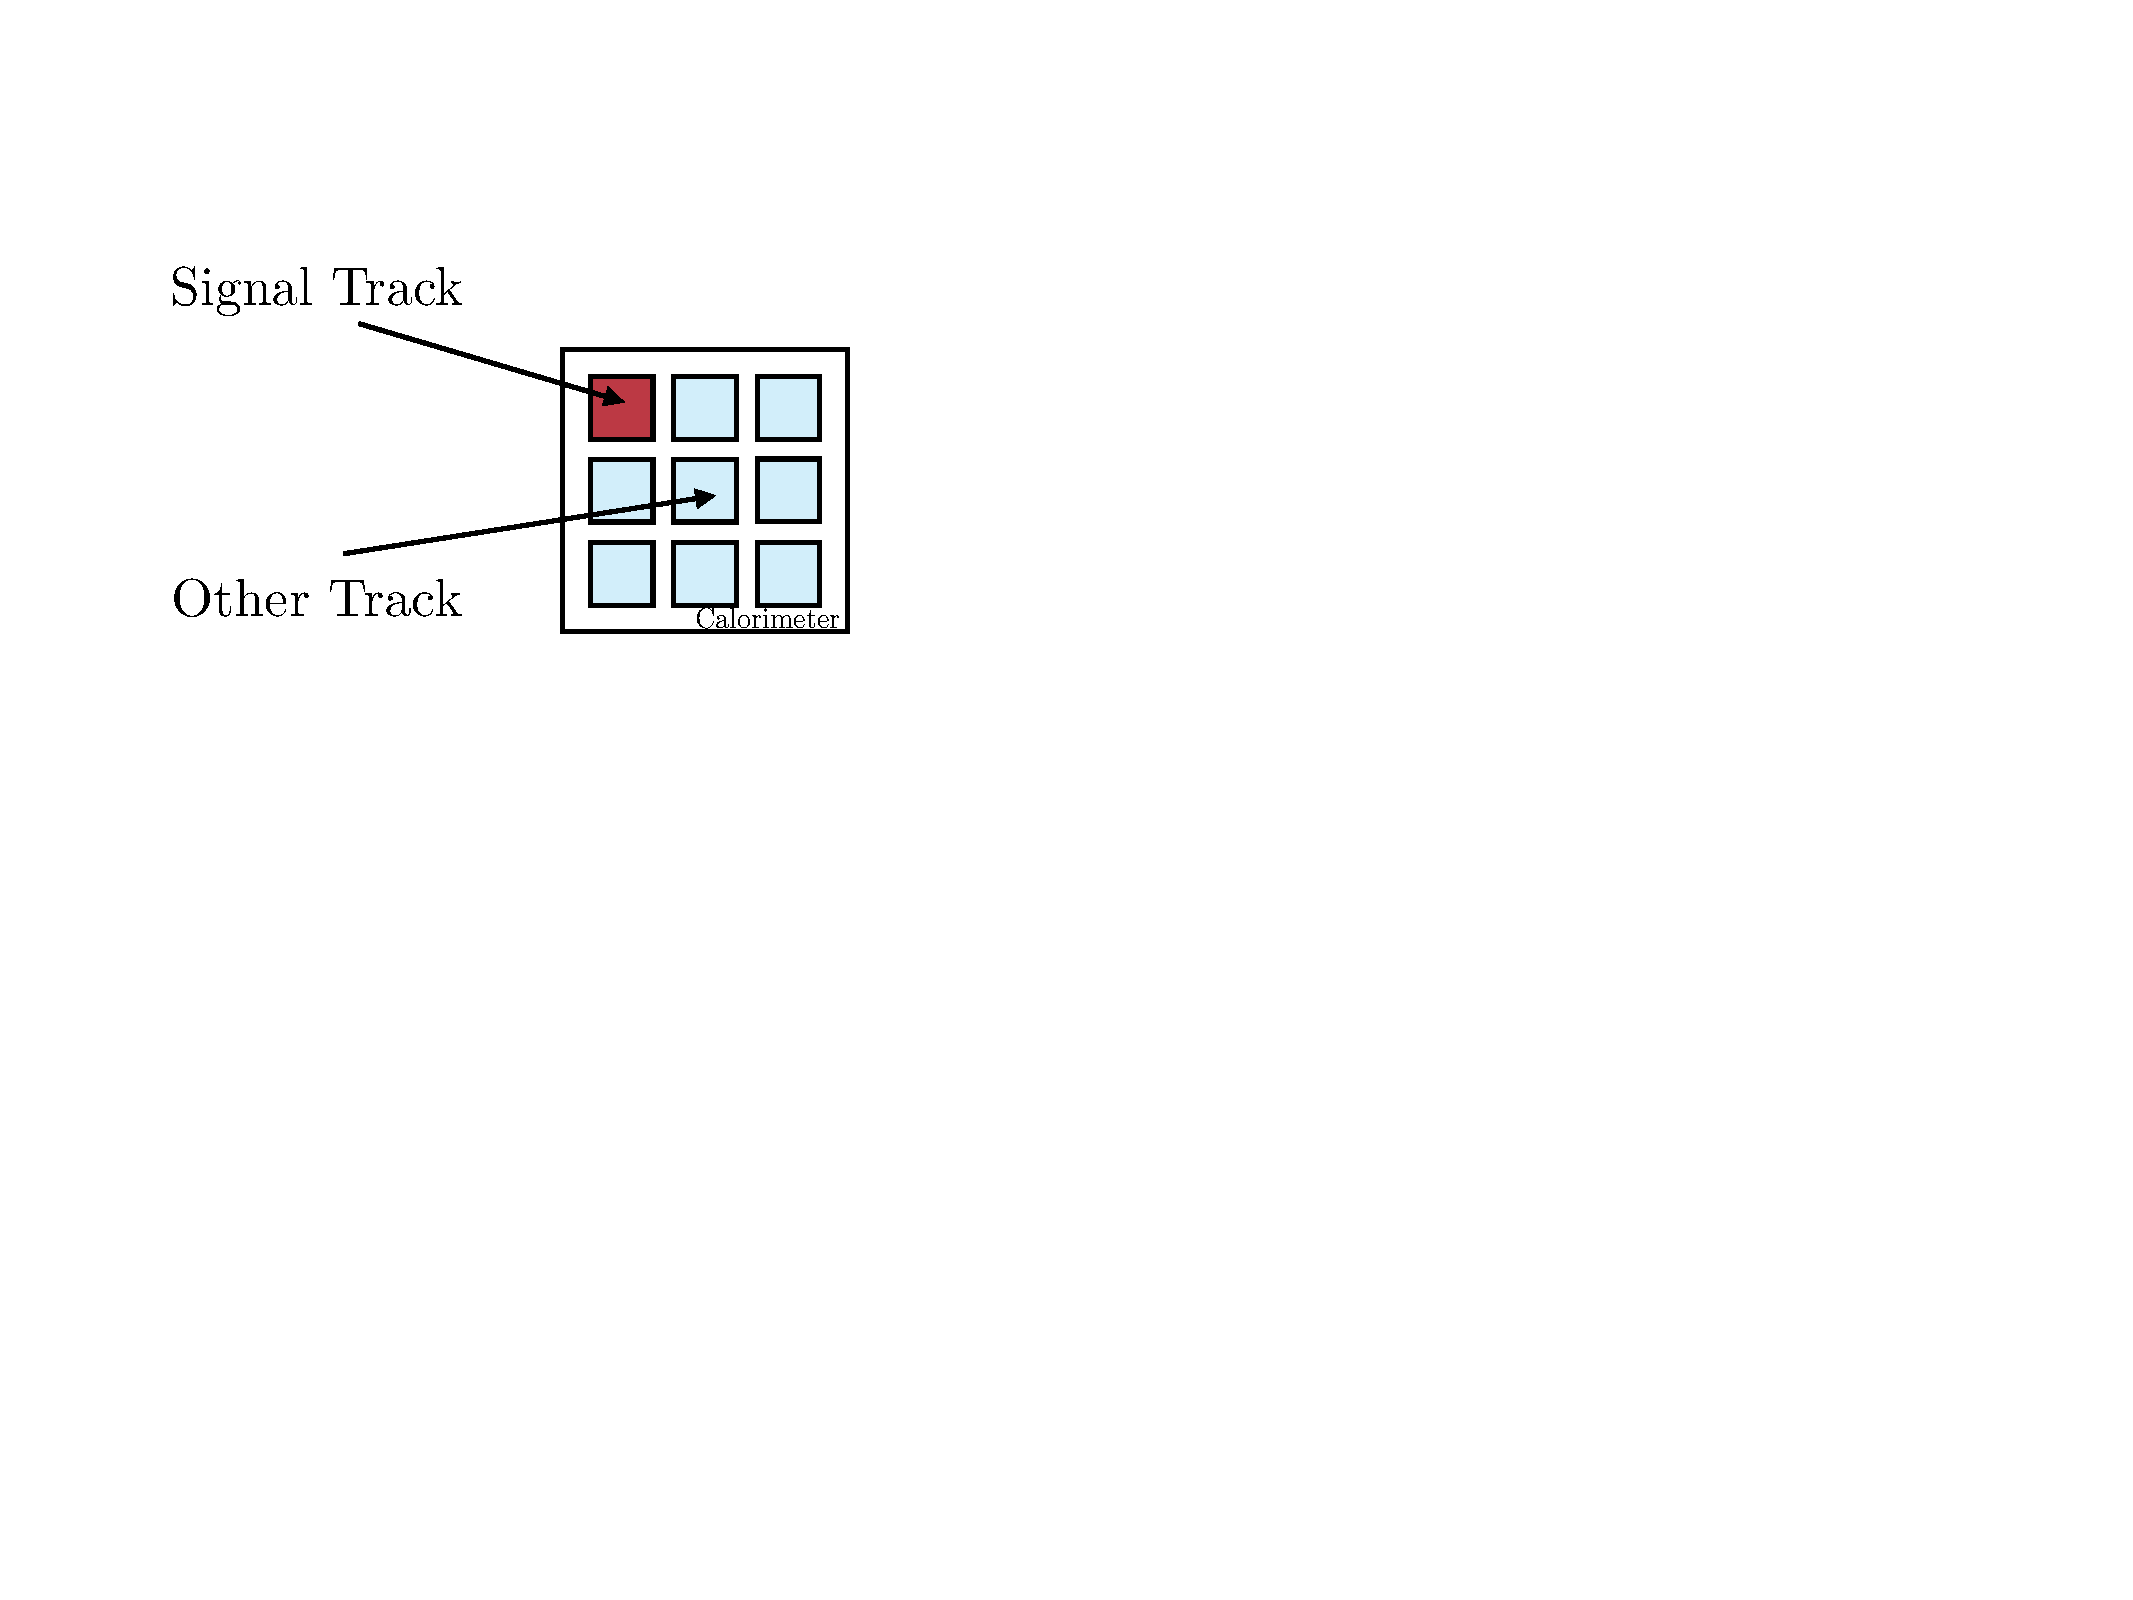
\includegraphics[width=1.0\textwidth]{figs/Selection/Tos.pdf}
        \caption{\texttt{TOS}}
        \label{fig:TOS}
    \end{subfigure}%
    \begin{subfigure}[t]{0.4\textwidth}
        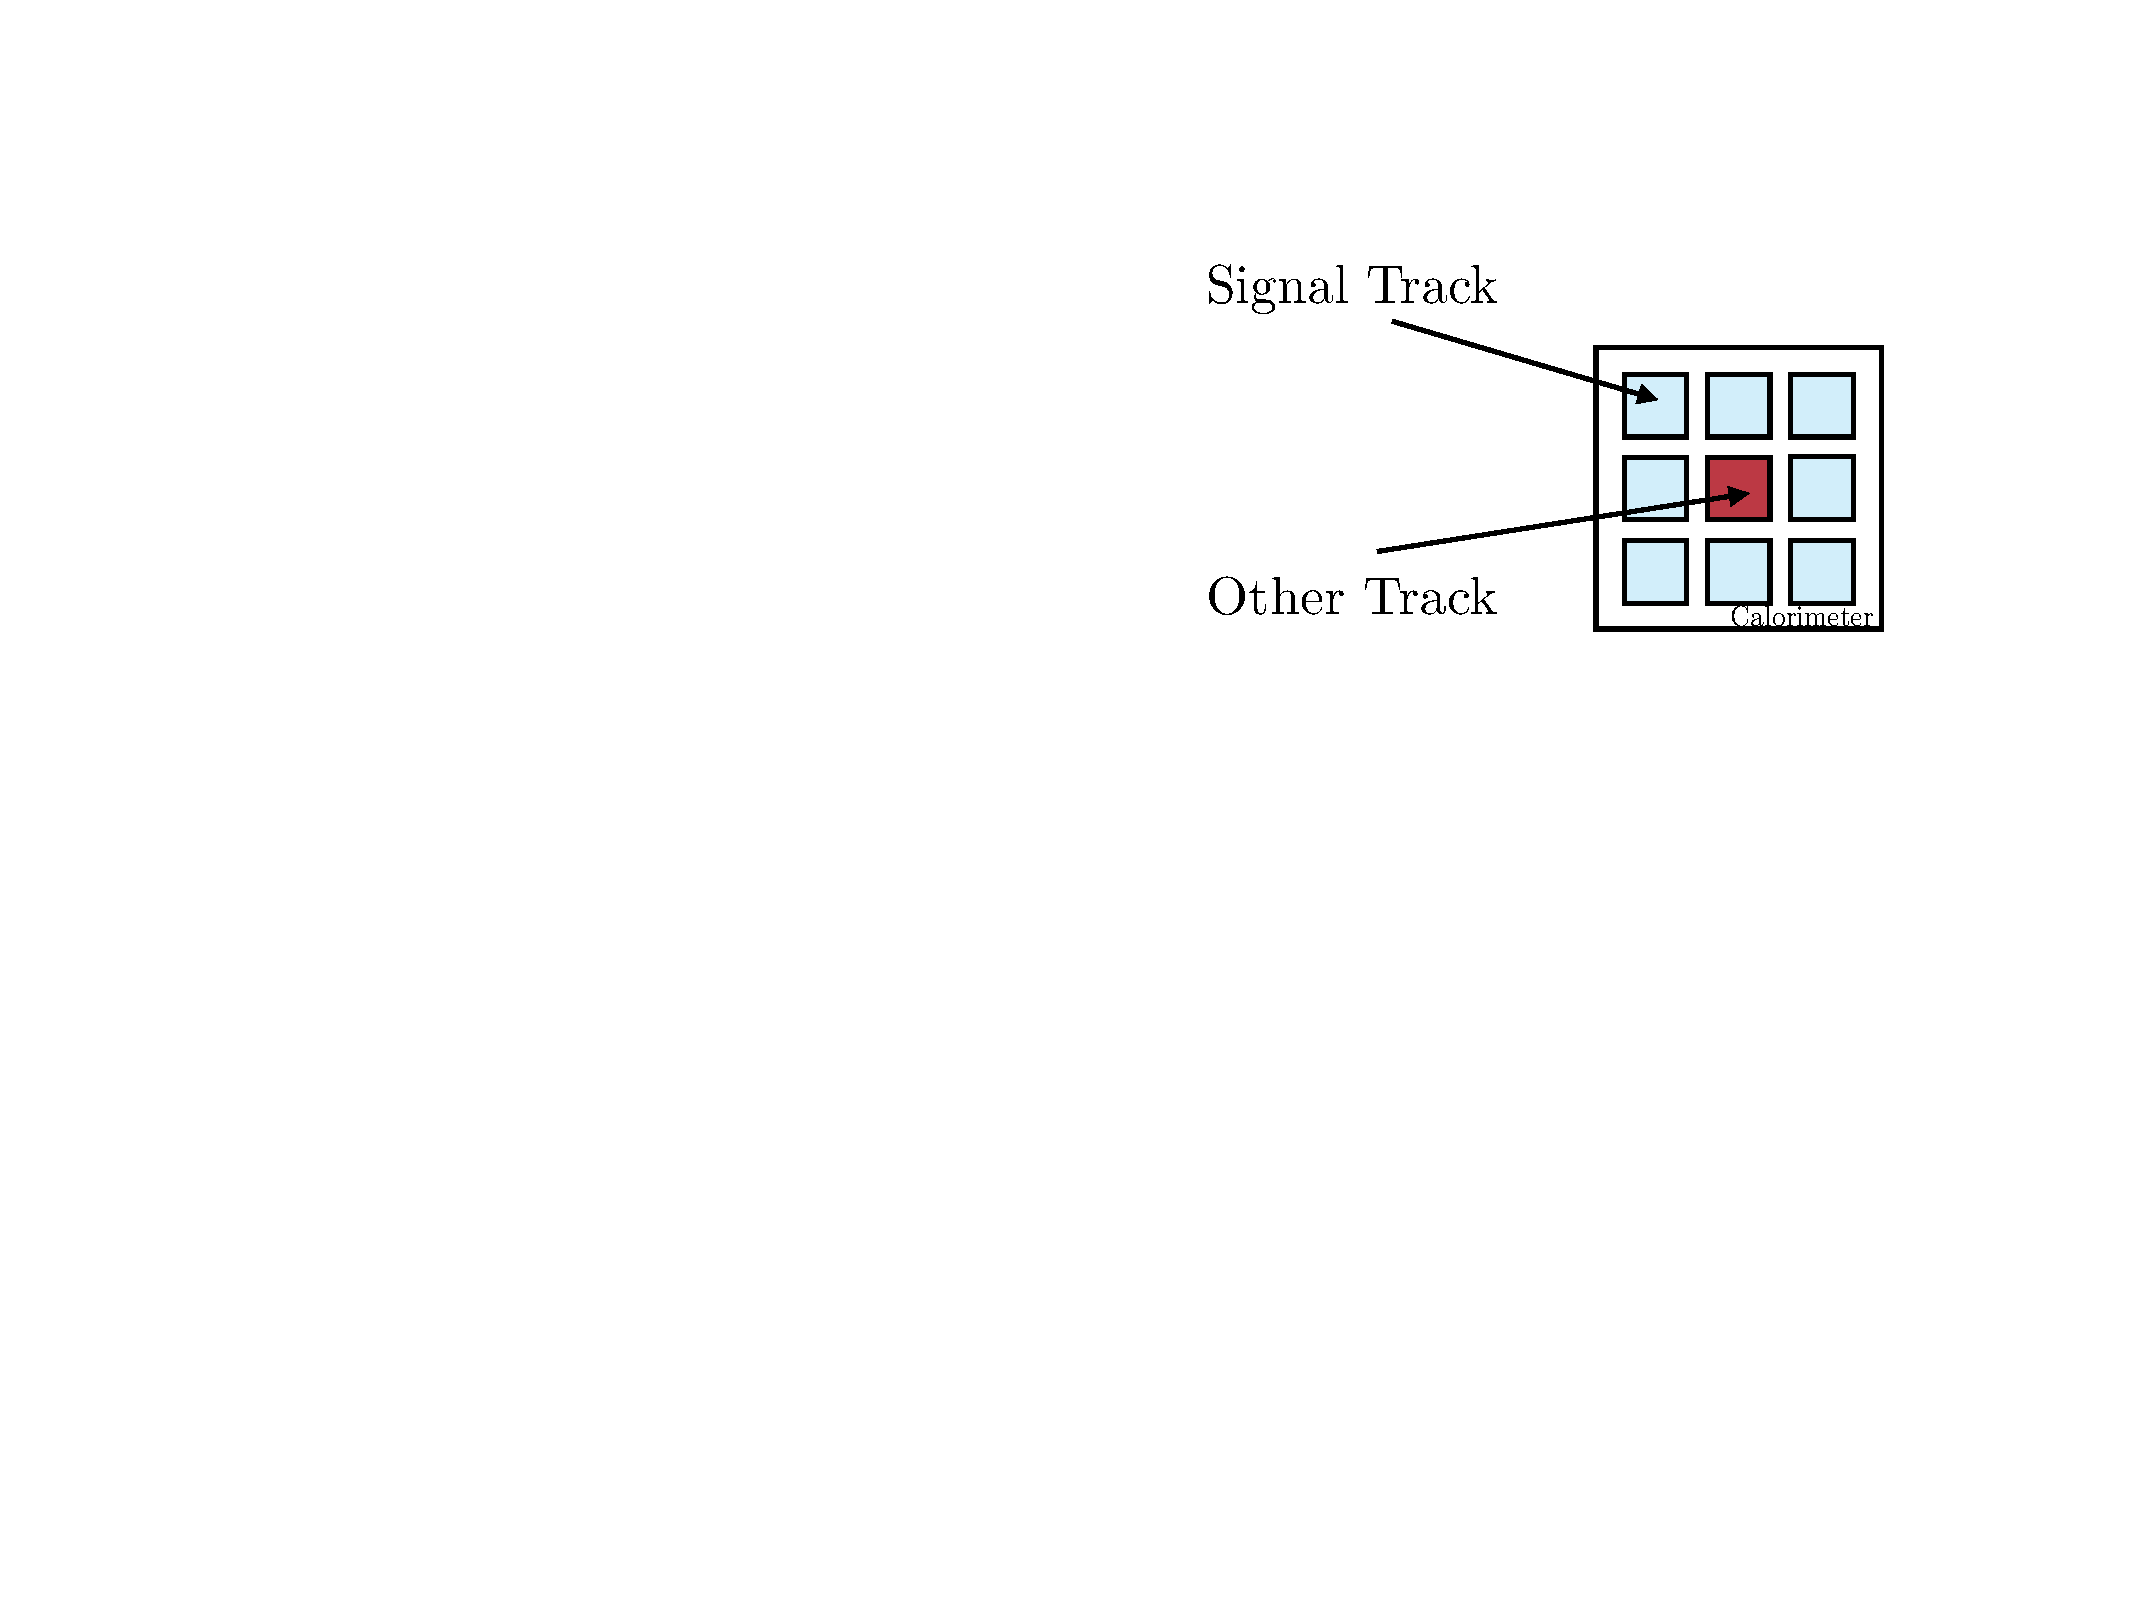
\includegraphics[width=1.0\textwidth]{figs/Selection/Tis.pdf}
        \caption{\texttt{TIS}}
        \label{fig:TIS}
    \end{subfigure}\\
    \begin{subfigure}[t]{0.4\textwidth}
        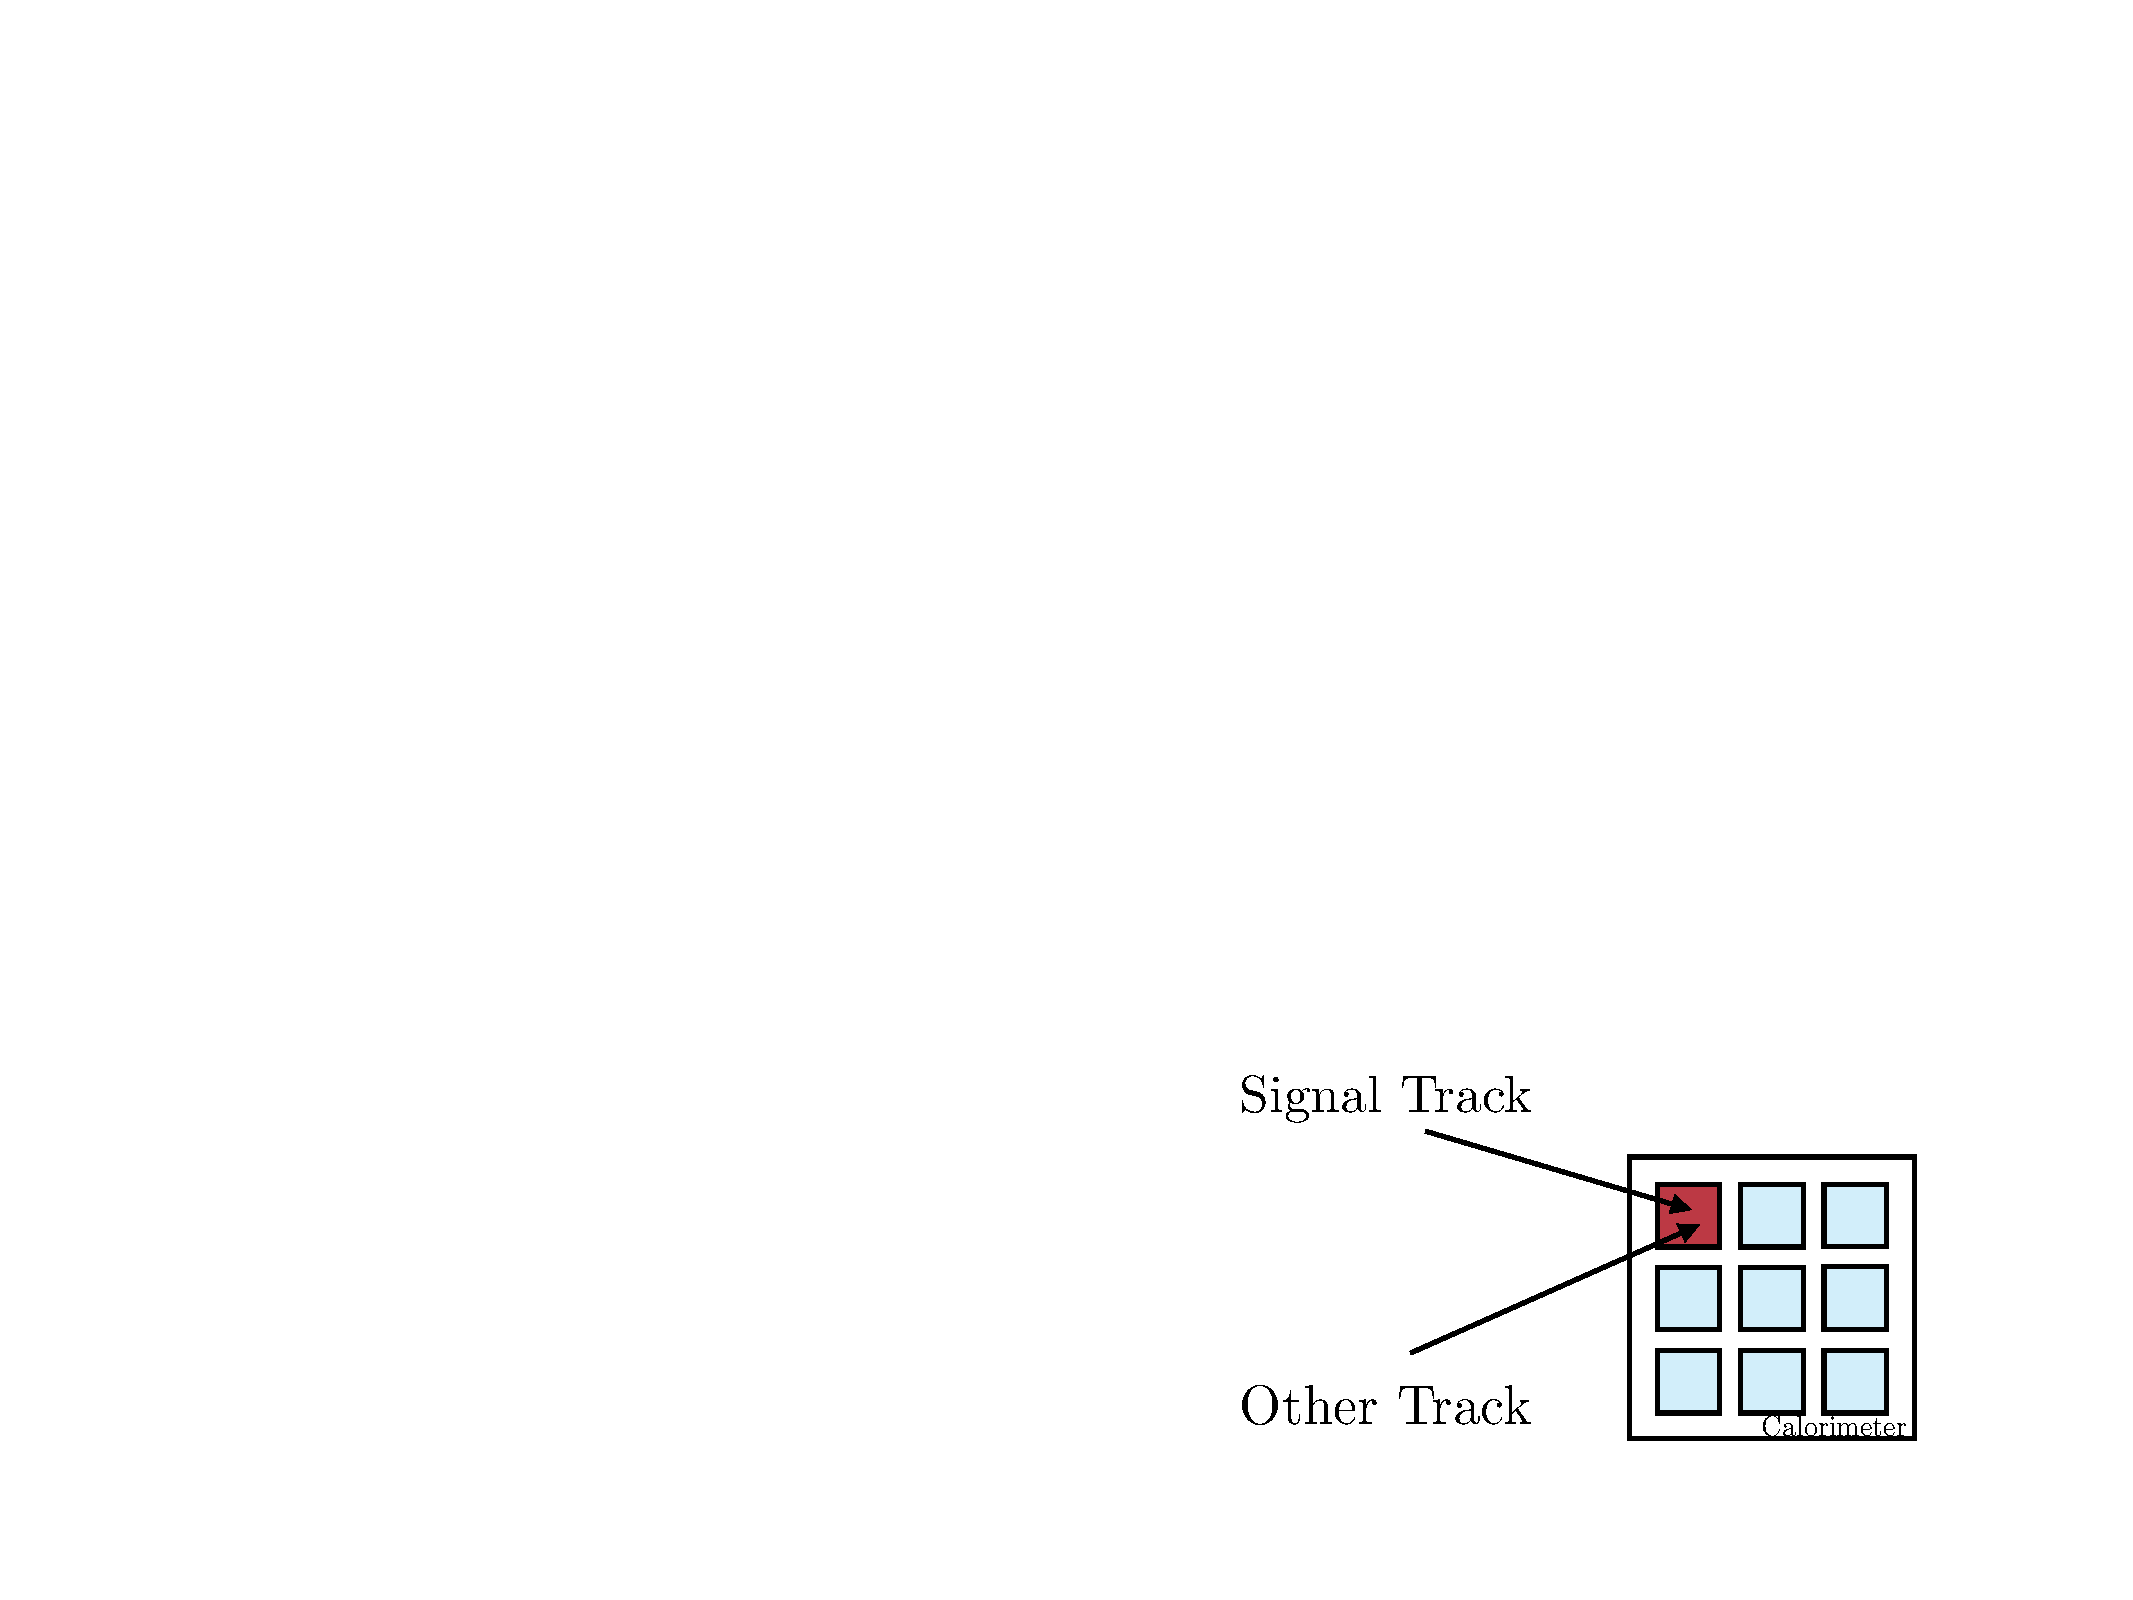
\includegraphics[width=1.0\textwidth]{figs/Selection/Tob.pdf}
        \caption{\texttt{TOB}}
        \label{fig:TOB}
    \end{subfigure}
    \begin{subfigure}[t]{0.4\textwidth}
        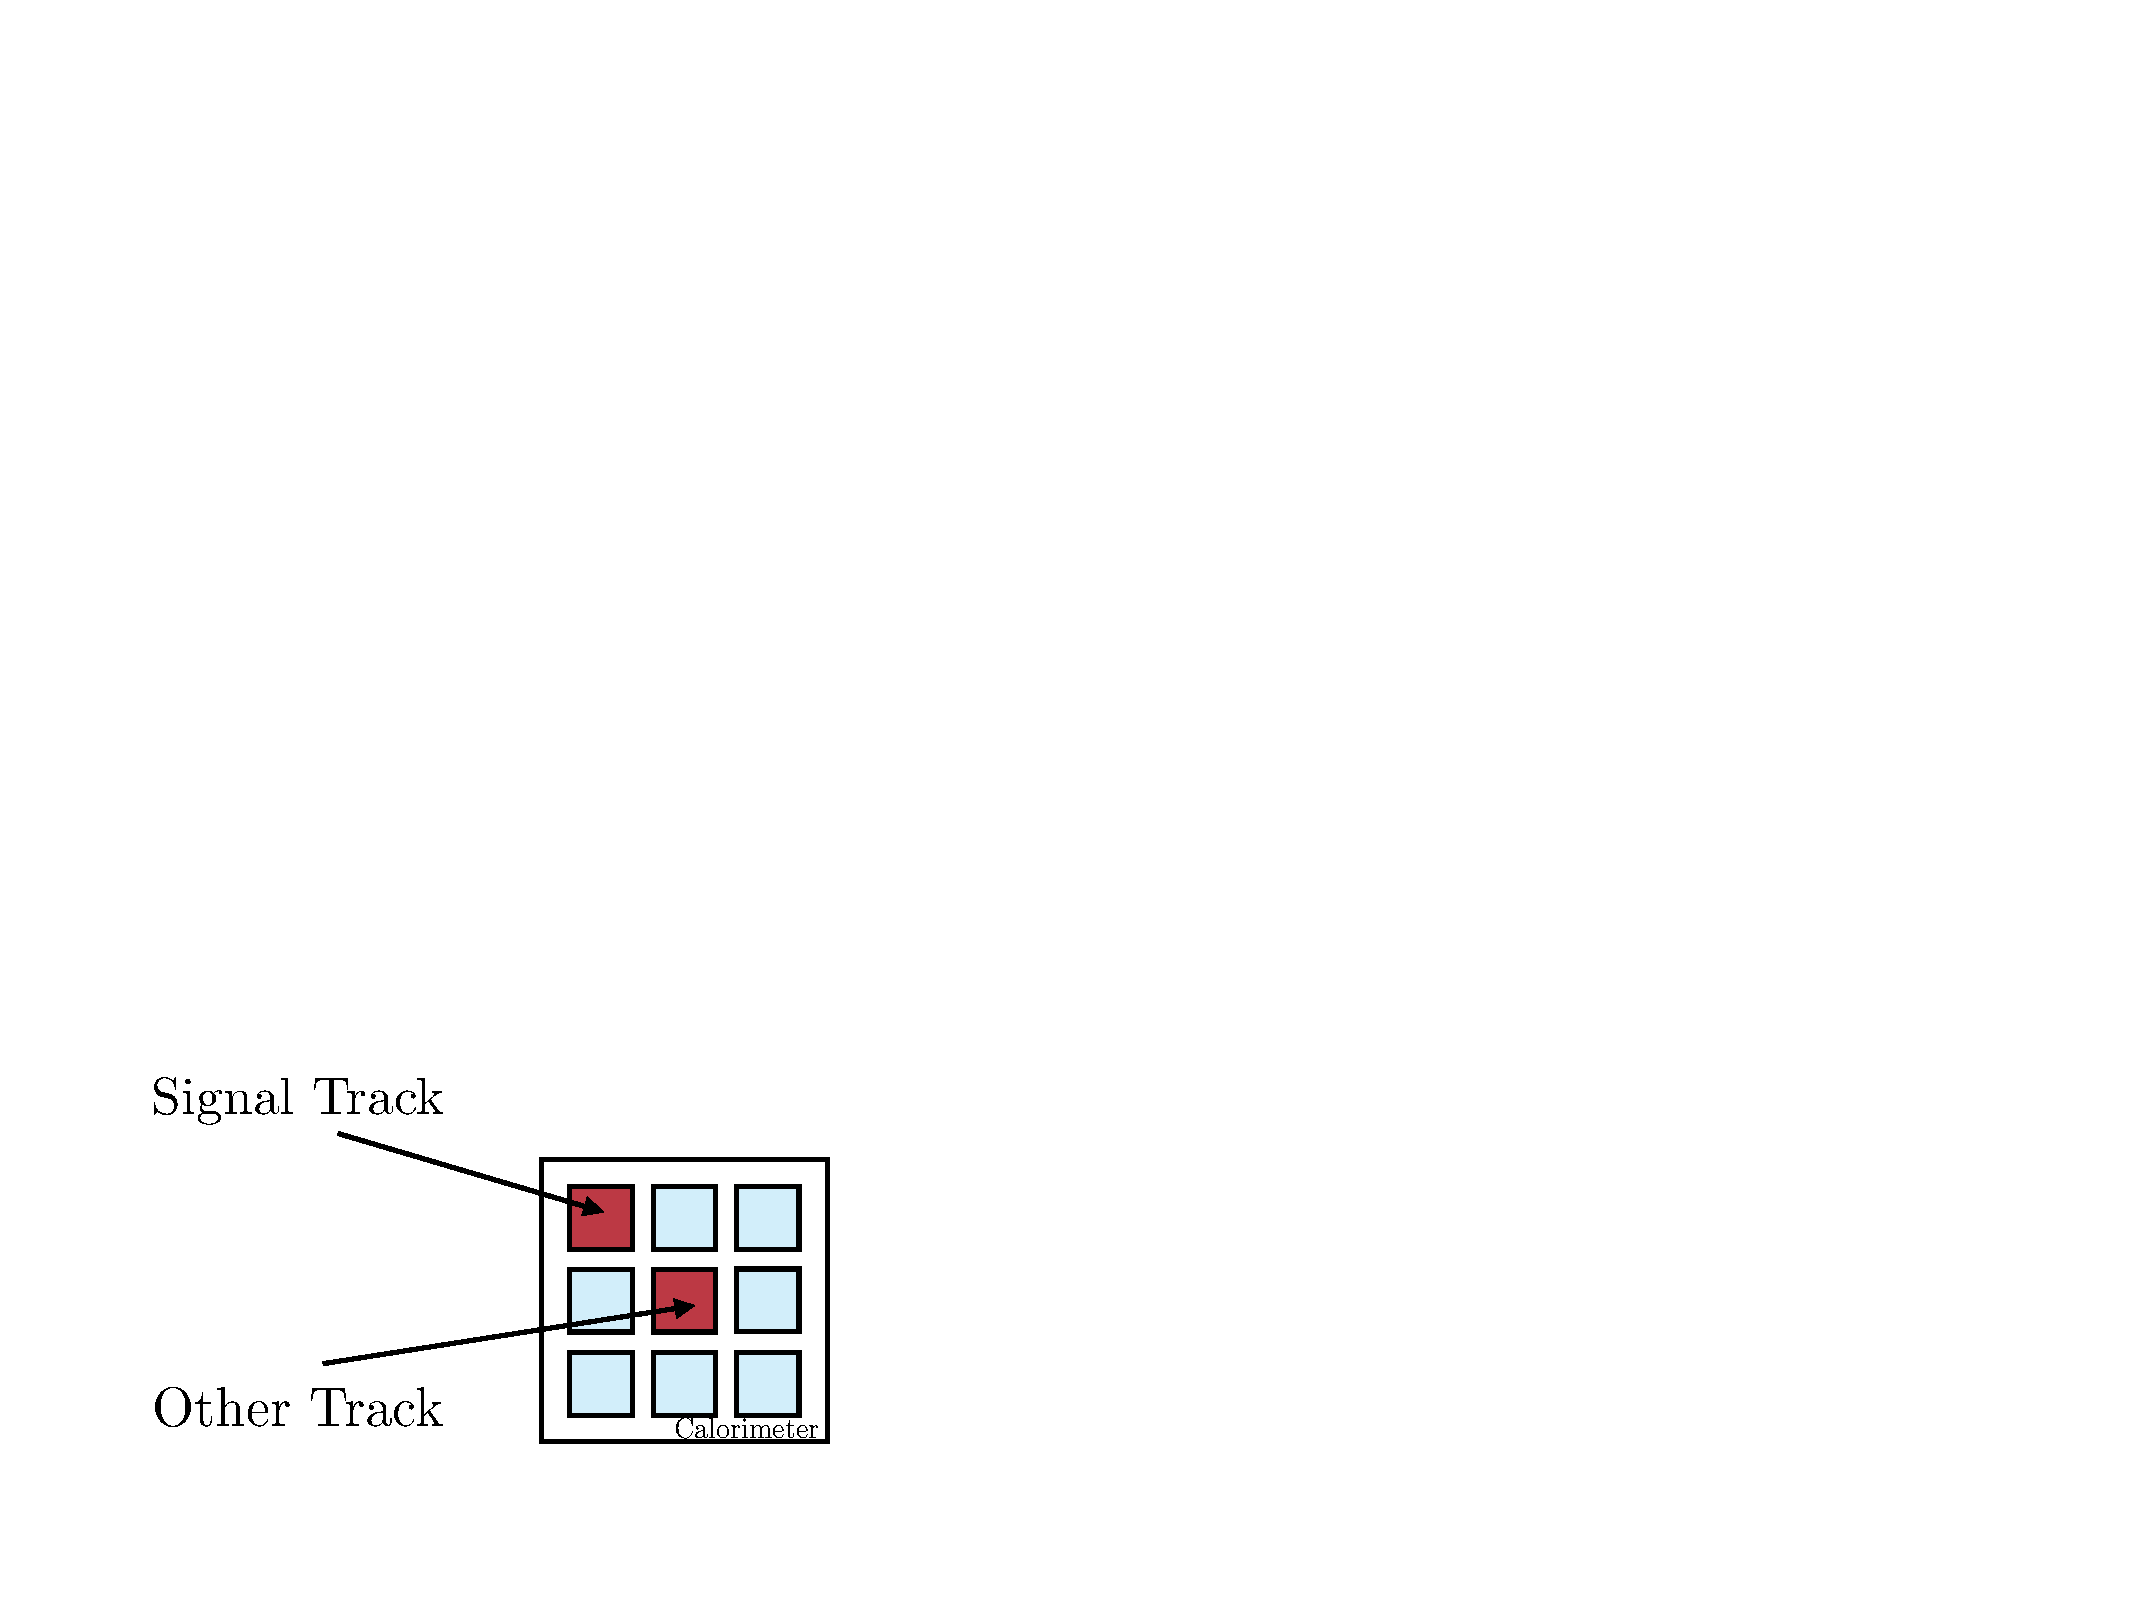
\includegraphics[width=1.0\textwidth]{figs/Selection/TisTos.pdf}
        \caption{\texttt{TOS} and \texttt{TIS}}
        \label{fig:TOSandTIS}
    \end{subfigure}\\
    \caption{Simple schematics of the different trigger matching possibilities, illustrated with one signal track and one non-signal track. Cells with a deposit above the trigger threshold are shown in red. }
    \label{fig:tistostobbing}   
\end{figure}
%%%%%%%%%%%%%%%%%%%%%%%%%%%%%%%%%%%%%%%%%%%%%%%%%%%%%%%%%%


At the hardware trigger stage, the selected candidates are required to be \texttt{TOS} with respect to the hadronic trigger \texttt{L0Hadron}. This ensures the selected candidates were retained due to corresponding deposits in the hadronic calorimeter. 
Alternatively, the logical `or' of each of the hardware sub-systems is combined into a global hardware trigger called \texttt{L0Global}.
Candidates are selected if they are \texttt{TIS} with respect to this combination.
%Alternatively, candidates are selected if they are \texttt{TIS} with respect to the global hardware trigger \texttt{L0Global}; any of the hardware trigger subsystems can contribute to the \texttt{L0Global} decision. 
This allows a second source of decays; those events where the other \bquark quark in a \bquark\bquarkbar pair production has been selected by the trigger. 


This allows candidates that have been retained due another highly energetic decay in the same event to contribute. This could be the decay of hadron resulting from the other \bquark quark in a \bquark\bquarkbar pair production. 

The relative fractions of simulated decays selected by these \texttt{L0Hadron TOS} and \texttt{L0Global TIS} requirements for \decay{\Bp}{\Dsp\phiz} decays decaying to various \Dsp final states are shown in Table~\ref{tab:tis_tos_fractions}. The fractions are normalised to the total number of signal decays passing the \texttt{L0Hadron TOS} or \texttt{L0Global TIS} trigger requirements. 

% \begin{table}[h]
%    \centering
%       \begin{tabular}{lcccc}
%          \hline
%          \Dsp decay mode                &  \texttt{TOS} \& !\texttt{TIS} & \texttt{TIS}\&!\texttt{TOS} &  \texttt{TIS}\&\texttt{TOS}&  \texttt{TIS} or \texttt{TOS}\\
%          \hline 
%          \decay{\Dsp}{\Kp\Km\pip}       & $34.0\%$                   &$40.0\%$                   &$22.9\%$                   &$96.9\%$\\
%          \decay{\Dsp}{\Kp\pim\pip}      & $34.9\%$                   &$38.3\%$                   &$23.8\%$                   &$96.9\%$\\
%          \decay{\Dsp}{\pip\pim\pip}     & $35.9\%$                   &$37.5\%$                   &$23.5\%$                   &$96.9\%$\\
%          \hline
%       \end{tabular}
%    
%    \caption{The fraction of simulated \decay{\Bp}{\Dsp\phiz} decays in each of the hardware trigger categories for the Run I conditions. Here \texttt{TOS} refers to candidates found to be \texttt{TOS} with respect to the \texttt{L0Hadron} trigger, and \texttt{TIS} to candidates found to be \texttt{TIS} with respect to the \texttt{L0Global} requirement. The percentages are given relative to the number of decays passing the reconstruction requirements.}
%    \label{tab:tis_tos_fractions}
% \end{table}
\begin{table}[h]
   \centering
      \begin{tabular}{lccc}
         \hline
         \Dsp decay mode                &  \texttt{TOS} \& !\texttt{TIS} & \texttt{TIS}\&!\texttt{TOS} &  \texttt{TIS}\&\texttt{TOS}\\
         \hline 
         \decay{\Dsp}{\Kp\Km\pip}       & $35.1\%$                   &$41.2\%$                   &$23.7\%$       \\
         \decay{\Dsp}{\Kp\pim\pip}      & $38.0\%$                   &$36.7\%$                   &$25.3\%$       \\
         \decay{\Dsp}{\pip\pim\pip}     & $41.3\%$                   &$31.9\%$                   &$26.8\%$       \\
         \hline
      \end{tabular}
   
   \caption{The fraction of simulated \decay{\Bp}{\Dsp\phiz} decays in each of the hardware trigger categories for the Run I conditions. Here \texttt{TOS} refers to candidates found to be \texttt{TOS} with respect to the \texttt{L0Hadron} trigger, and \texttt{TIS} to candidates found to be \texttt{TIS} with respect to the \texttt{L0Global} requirement. The percentages are given relative to the total number of decay selected by the logical `or' of the two requirements.}
   \label{tab:tis_tos_fractions}
\end{table}

The software trigger stage is split into two parts, \hltone and \hlttwo.
The first stage, \hltone, performs pattern recognition on hits in the \velo and extrapolates tracks forward to the other tracking stations. At least one well reconstructed track is required. This means the track must be significantly displaced from the primary interaction and with $\pt > 1.7 \gevc$. In Run II, this trigger was reimplementing using a multivariate analysis. 

%????????????????????????
% An second algorithm is included to select pairs of high transverse momentum tracks that form a vertex that is displaced from the primary interaction. The signal candidate is required to be \texttt{TOS} with respect to these trigger lines such that two of the $\Dsp h^{+}h^{-}$ candidate tracks passes this requirement.   
%????????????????????????

At the second software stage, \hlttwo, two different algorithms are used to select $\Dsp h^{+}h^{-}$ candidates for this analysis.
The first one uses a multivariate algorithm~\cite{BBDT} to identify the presence of a secondary vertex that has two, three or four tracks and is displaced from any PV. 
%At least one of these charged particles must have a transverse momentum $\pt > 1.7\gevc$ and be inconsistent with originating from a PV. %\chisqip with respect to any primary interaction greater than 16, where \chisqip is defined as the difference in \chisq of a given PV reconstructed with and without the considered track.
This trigger algorithm is referred to as the topological trigger.
The second algorithm selects $\phiz$ candidates decaying to two charged kaons. Each kaon must have a transverse momentum $\pt > 0.8\gevc$ and be inconsistent with originating from a PV. The invariant mass of the kaon pair must be within $20\mevcc$ of the known \phiz mass~\cite{PDG2016}.
This inclusive \phiz line is used to maximise the selection efficiencies as \phiz mesons can contribute directly to \decay{\Bp}{\Dsp\phiz} decays, as well as via the large fractions of \decay{\Dsp}{\phiz\pip} decays that contribute to the \decay{\Dsp}{\Kp\Km\pip} final state.
The relative fractions of simulated \decay{\Bp}{\Dsp\phiz} decays selected by these different trigger algorithms are listed in Table~\ref{tab:topo_incphi_fractions}. The \decay{\Dsp}{\Kp\Km\pip} simulation is generated using an amplitude model that includes the \decay{\Dsp}{\phiz\pip} contribution. As a result, it can be seen that the inclusive \phiz trigger algorithm helps to retain a larger fraction of decays. 

\begin{table}[h]
   \centering
      \begin{tabular}{lccc|c}
         \hline
         \Dsp decay mode                &  \texttt{Topo} \& !\texttt{Phi} & \texttt{Phi}\&!\texttt{Topo} &  \texttt{Topo}\&\texttt{Phi}&  \texttt{Topo} or \texttt{Phi}\\
         \hline 
         \decay{\Dsp}{\Kp\Km\pip}       & $50.9\%$                   &$4.6\%$                   &$43.1\%$                   &$98.7\%$\\
         \decay{\Dsp}{\Kp\pim\pip}      & $67.6\%$                   &$2.7\%$                   &$28.3\%$                   &$98.5\%$\\
         \decay{\Dsp}{\pip\pim\pip}     & $67.5\%$                   &$2.6\%$                   &$28.5\%$                   &$98.7\%$\\
         \hline
      \end{tabular}
   
   \caption{The fraction of simulated \decay{\Bp}{\Dsp\phiz} decays in each of the \hlttwo software trigger categories for the Run I conditions. Here \texttt{Topo} refers to candidates found to be \texttt{TOS} with respect to the topological algorithm, and \texttt{Phi} to candidates found to be \texttt{TOS} with respect to the inclusive \phiz algorithm. The fractions of selected decays are measured relative to the \hltone requirements.}
   \label{tab:topo_incphi_fractions}
\end{table}



\section{Offline selection}

Events passing any trigger requirement are saved to disk for processing offline. The stages of the offline reconstruction are detailed in this section.

\subsection{Selection requirements}
\label{sec:selectionrequirements}

The offline data samples selected by the online trigger system are reconstructed and then further processed in a procedure know within \lhcb as \emph{Stripping}. This centrally managed processing builds candidate topologies from tracks and neutral calorimeter objects in each event according to a set of predefined \emph{Stripping Lines}. Each line builds a specific candidate decay, applying a loose set of preselection requirements, including kinematic, geometric and invariant mass selections. 

The candidate \decay{\Bp}{\Dsp\phiz} and \decay{\Bp}{\Dsp\Kp\Km} decays are built using almost identical set of requirements due to the similar topologies of these decays. The \phiz meson has a lifetime of $(1.55\pm0.01)\times10^{-22}\sec$~\cite{PDG2016}, therefore the kaon decay products effectively originate at the \Bp decay vertex in a similar way to \decay{\Bp}{\Dsp\Kp\Km} decays.  The normalisation channel, \decay{\Bp}{\Dsp\Dzb}, is built similarly, however the difference in lifetime between the \Dzb and \phiz mesons necessitates slightly different selection requirements. The \Dzb meson has a lifetime of $(4.101\pm0.015)\times10^{-13}\sec$, allowing the meson to travel away from the \Bp decay vertex. Sketches of the signal and normalisation decay topologies are shown in Fig.~\ref{fig:topo}.

%%%%%%%%%%%%%%%%%%%%%%%%%%%%%%%%%%%%%%%%%%%%%%%%%%%%%%%%%%
\begin{figure}[!h]
    \centering
    \begin{subfigure}[t]{0.4\textwidth}
        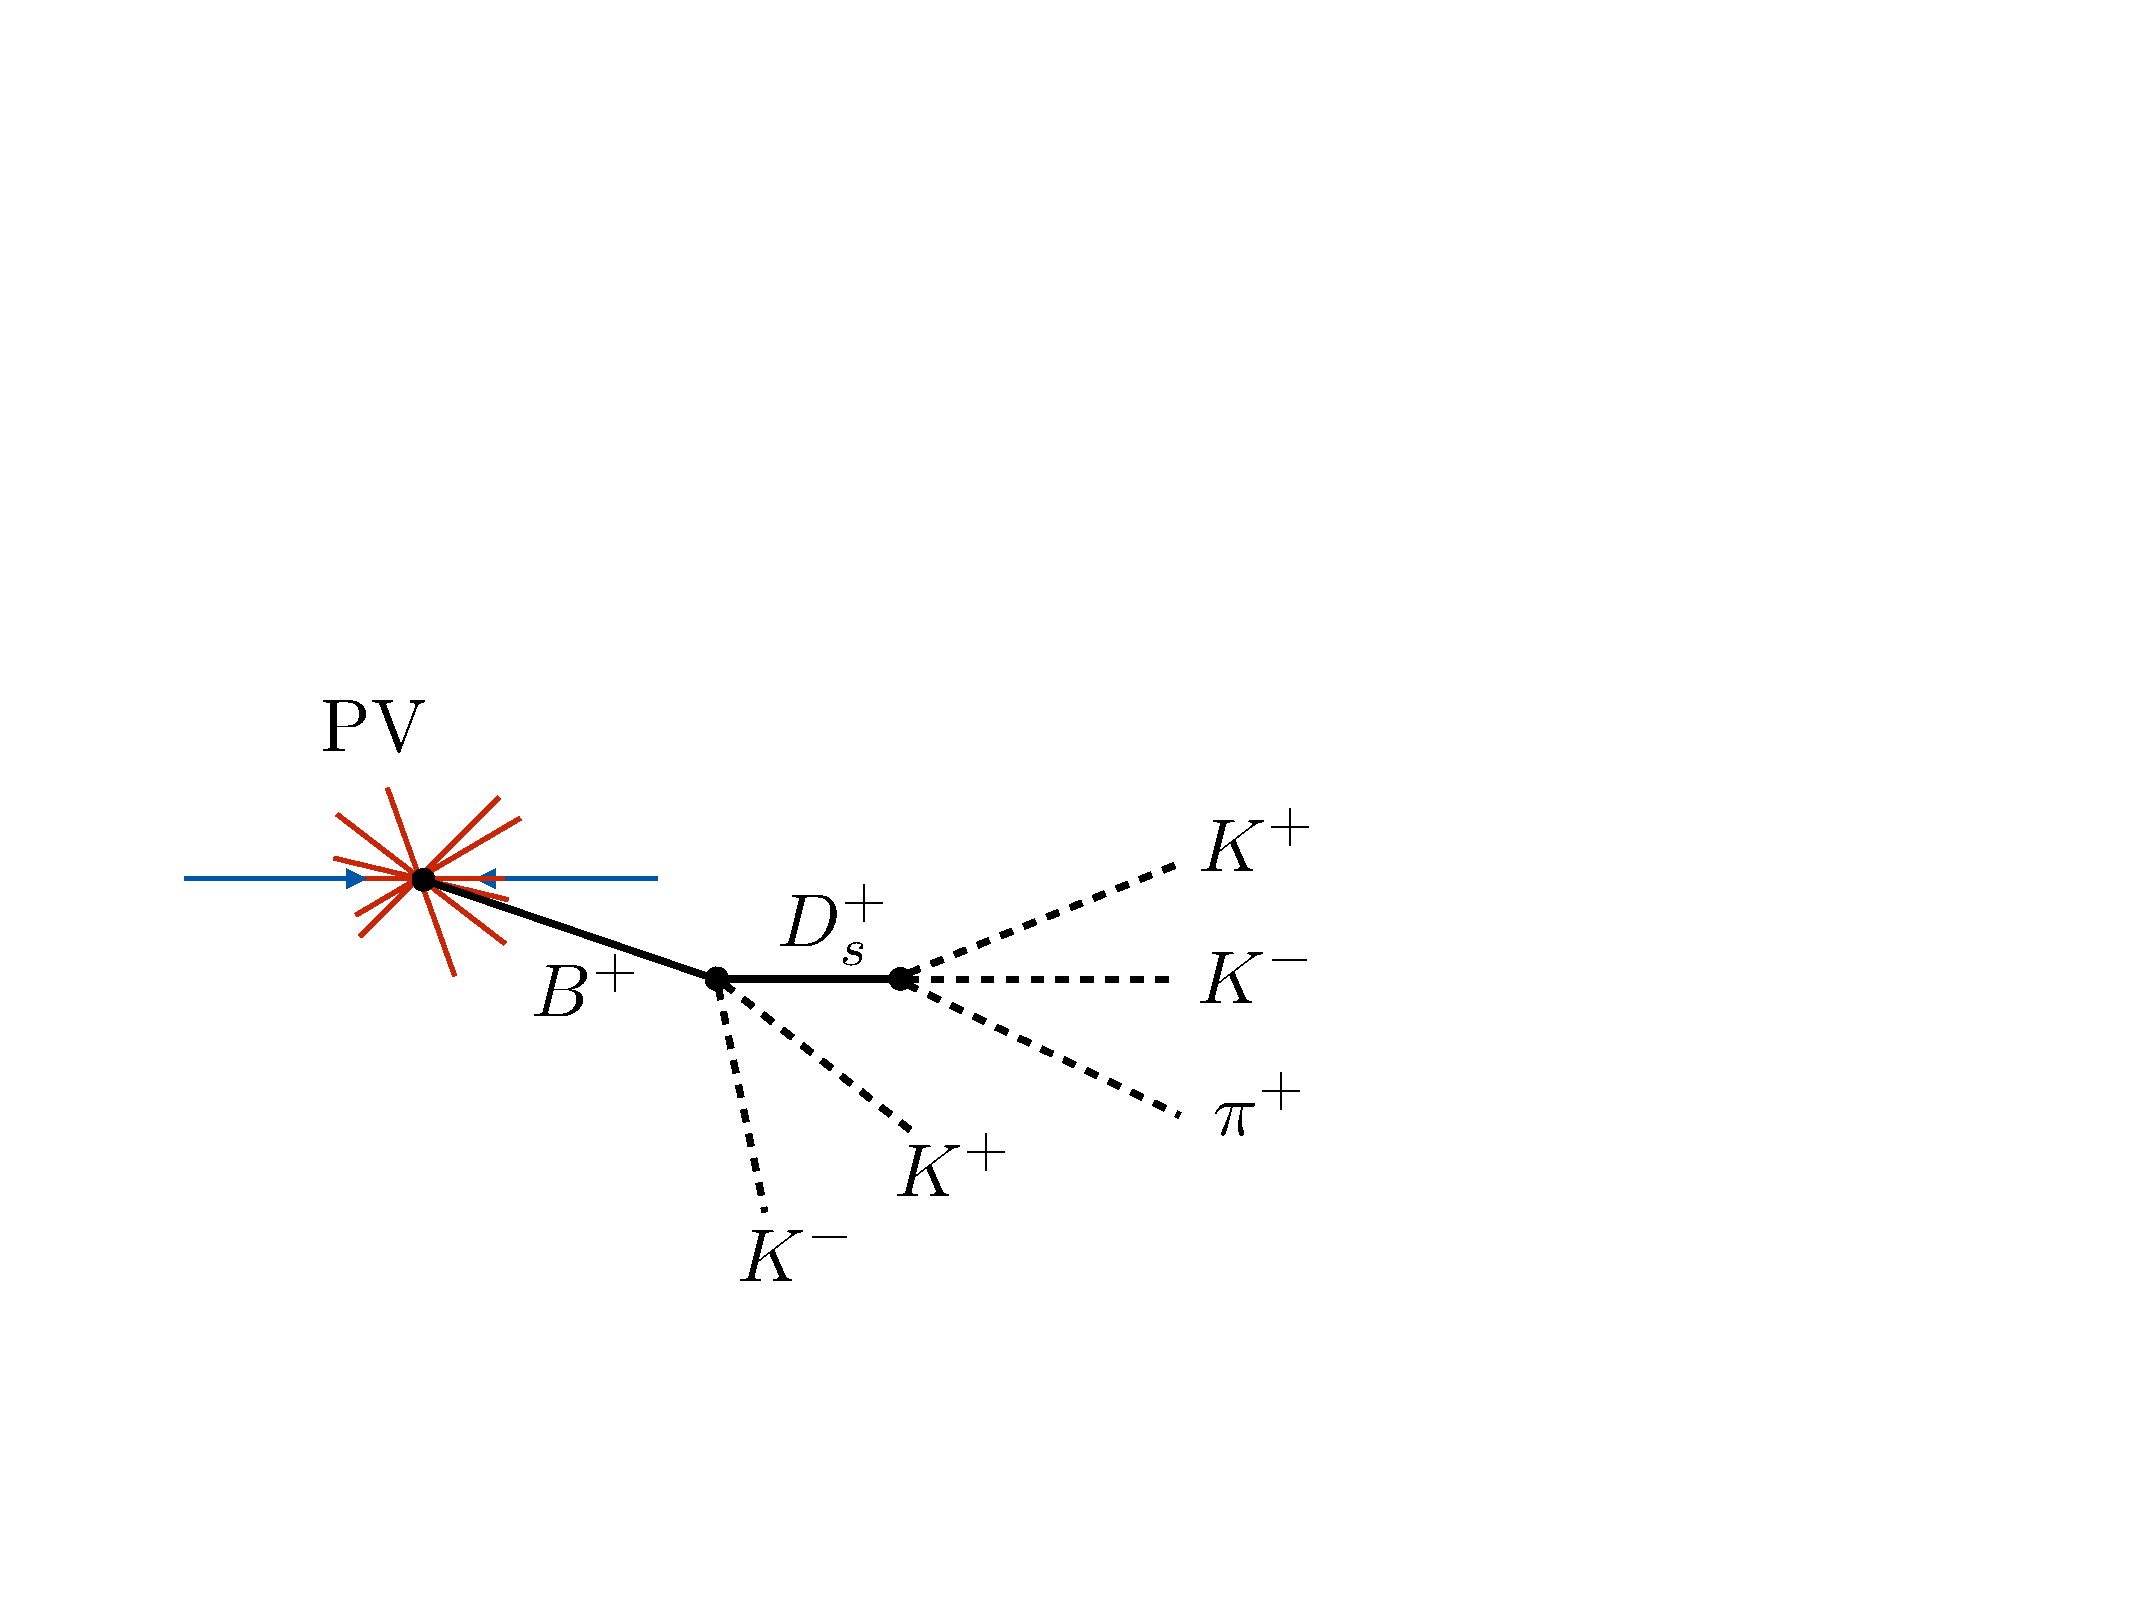
\includegraphics[width=1.0\textwidth]{figs/Selection/B2DsKK_topology.pdf}
        \caption{Signal decays}
    \end{subfigure}%
    \begin{subfigure}[t]{0.4\textwidth}
        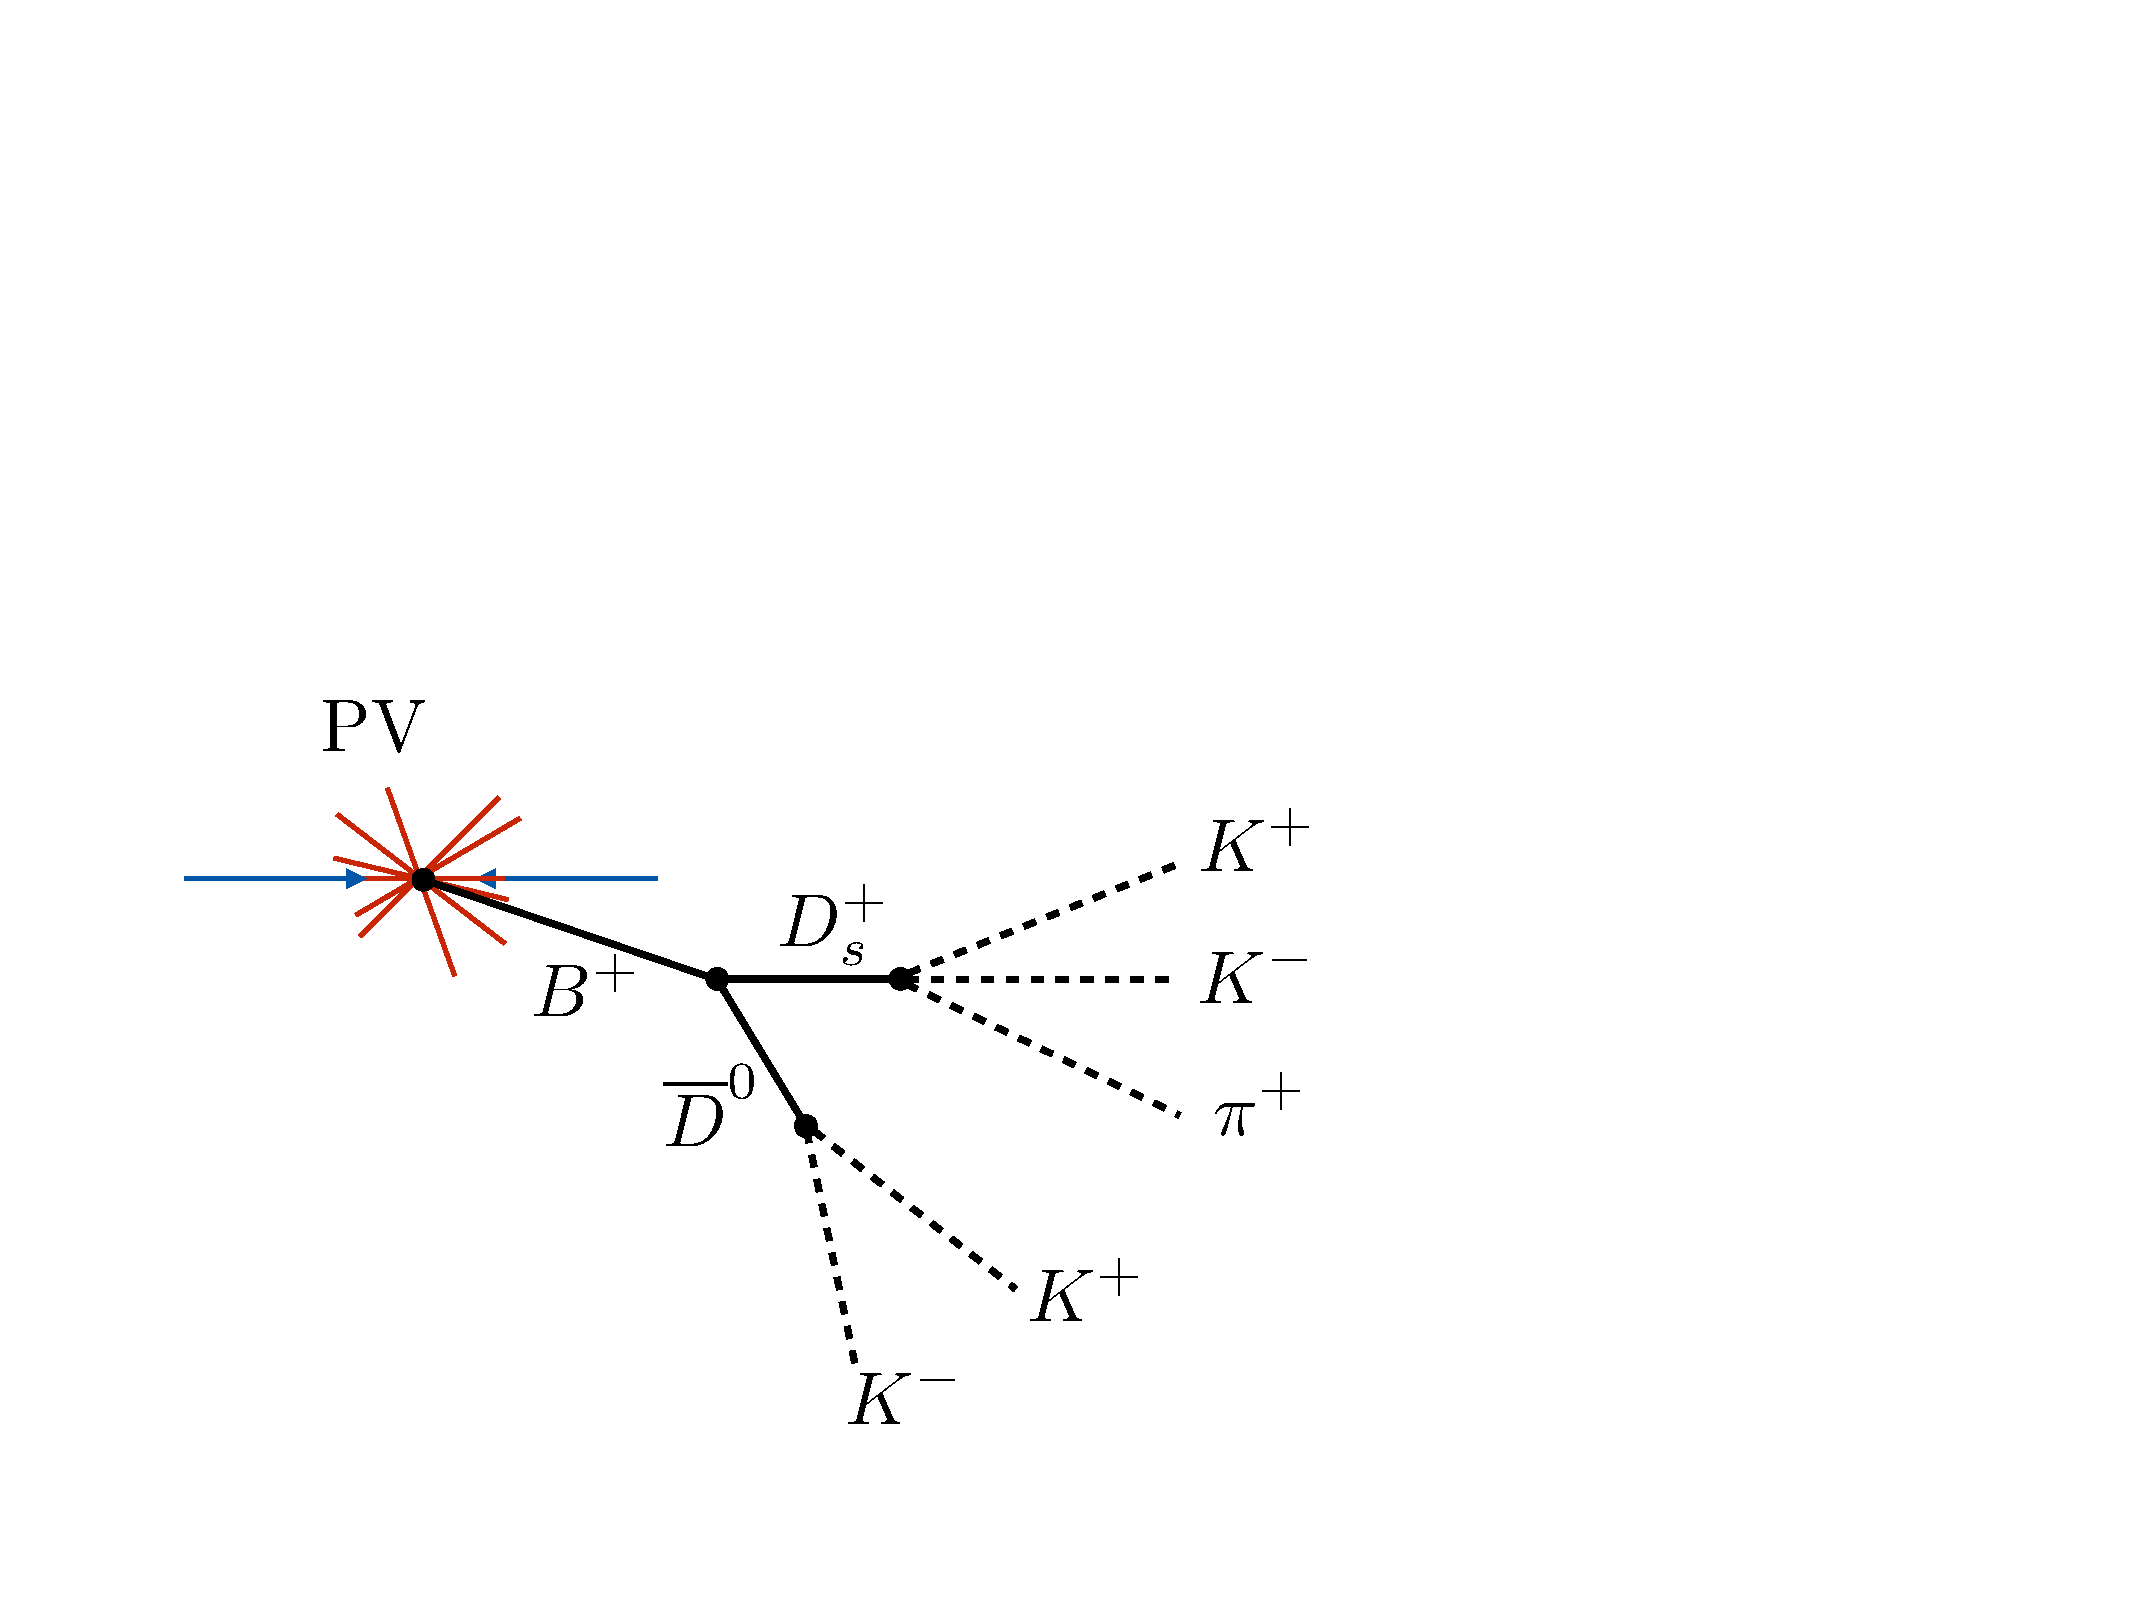
\includegraphics[width=1.0\textwidth]{figs/Selection/B2DsD0_topology.pdf}
        \caption{Normalisation decays}
    \end{subfigure}\\
    \caption{The signal and normalisation decay topologies. The collision of the two protons (blue) results in the primary collision vertex (PV). Many promptly produced tracks (red) originate at the PV. In both cases, the long-lived \Bp meson decay vertex is displaced from the PV. The long-lived charm mesons are also displaced from the \Bp meson decay vertex.}
    \label{fig:topo}   
\end{figure}
%%%%%%%%%%%%%%%%%%%%%%%%%%%%%%%%%%%%%%%%%%%%%%%%%%%%%%%%%%

The candidate \decay{\Bp}{\Dsp\Kp\Km} and \decay{\Bp}{\Dsp\phiz} signal decays and \decay{\Bp}{\Dsp\Dzb} normalisation decay are reconstructed in fully hadronic final states. Both the \Dzb and \phiz mesons are reconstructed using pairs of oppositely charged kaons. The branching fractions are $\BF(\decay{\Dzb}{\Kp\Km})= (3.97 \pm 0.07)\times 10^{-3}$ and $\BF(\decay{\phiz}{\Kp\Km})= (48.9 \pm 0.5)\%$ respectively~\cite{PDG2016}. Although the similar two-body hadronic decay \decay{\Dz}{\Km\pip} has a larger branching fraction than mode chosen for the normalisation channel, $\BF(\decay{\Dz}{\Km\pip})= (3.89 \pm 0.04)\%$, sharing the same final state helps to reduced systematic uncertainties in the ratio of selection efficiencies. Many differences in how pions and kaons interact with the detector can be neglected as they would affect the signal and normalisation channel in the same way.
The \Dsp mesons used in the search for \decay{\Bp}{\Dsp\Kp\Km} decays are reconstructed using the \decay{\Dsp}{\Kp\Km\pip} decay. The search for the rarer \decay{\Bp}{\Dsp\phiz} decay additionally includes the modes \decay{\Dsp}{\pip\pim\pip} and \decay{\Dsp}{\Kp\pim\pip} to increase the sensitivity of the search. The branching fractions for these decays are listed in Table~\ref{tab:dsbranchingfractions}. In each instance the normalisation channel is reconstructed using the same \Dsp decay mode as the signal.  


\begin{table}[h]
   \centering
      \begin{tabular}{lccc}
         \hline
         Decay                            &\Dsp\phiz   &\Dsp\Kp\Km   &  Branching fraction \\
         \hline 
         \decay{\Dsp}{\Kp\Km\pip}         &\checkmark   &\checkmark   & $5.45 \pm 0.17 \%$ \\
         \decay{\Dsp}{\pip\pim\pip}       &\checkmark   & -  & $1.09 \pm 0.05 \%$ \\
         \decay{\Dsp}{\Kp\pim\pip}        &\checkmark   & -   & $0.66 \pm 0.04 \%$ \\
         \hline
      \end{tabular}
   
   \caption{The branching fractions for the different \Dsp decay modes used to reconstruct the signal and normalisation modes. The \Dsp decay modes contributing to the different searches are highlighted.}
   \label{tab:dsbranchingfractions}
\end{table}

%The searches for \decay{\Bp}{\Dsp\phiz} and \decay{\Bp}{\Dsp\Kp\Km} decays employ the use of two different \emph{Stripping Lines} as detailed in Table~\ref{tab:strippinglines}. These differ only in the invariant mass window applied to the $\Kp\Km$ pair used to reconstruct the $\phi$ meson, and in the number of \Dsp decay modes included: the \decay{\Bp}{\Dsp\Kp\Km} line only reconstructs the Cabibbo Favoured (CF) \decay{\Dsp}{\Kp\Km\pip} decay. The \emph{Stripping Line} used to select the normalisation channel \decay{\Bp}{\Dsp\Dzb} is also included in Table~\ref{tab:strippinglines}. This has slightly different requirements allowing the \Dzb meson decay vertex to be be displaced from the \Bp meson decay vertex.


The selection of candidates makes requirements on many different distinguishing characteristics. The definitions of the relevant quantities are as follows:  
\begin{description}
\item \textbf{Mass, $m(X)$:} the invariant mass of the particle, or combination of particles, $X$. 
\item \textbf{Momentum, \ptot:} the magnitude of the total momentum of the particle.
\item \textbf{Transverse momentum, \pt:} The component of the total momentum, \ptot, perpendicular to the proton beam axis (the $z$-axis).
\item \textbf{Decay Time, $\tau$:} the time taken for the candidate to travel from its production vertex to its decay vertex.
\item \textbf{Decay products' \pt scalar sum, $\sum{|\pt|}$:} the sum of the magnitudes of the transverse momentum of the decay products.
\item \textbf{Vertex quality, $\chi^{2}_{\text{VTX}}$:} the minimised value of $\chi^{2}$ per degree of freedom, $\chi^{2}/N_{\text{DOF}}$, as determined in the fit to the vertex location.
\item \textbf{Track quality, $\chi^{2}_{\text{TRK}}$:} the minimised value of $\chi^{2}/N_{\text{DOF}}$ as determined in the fit to the track hits.
\item \textbf{Impact parameter, $\text{IP}$:} The shortest distance between a given extrapolated track direction and a vertex location, as shown in Fig.~\ref{fig:impact_parameter}. 

%%%%%%%%%%%%%%%%%%%%%%%%%%%%%%%%%%%%%%%%%%%%%%%%%%%%%%%%%%
\begin{figure}[!h]
    \centering
    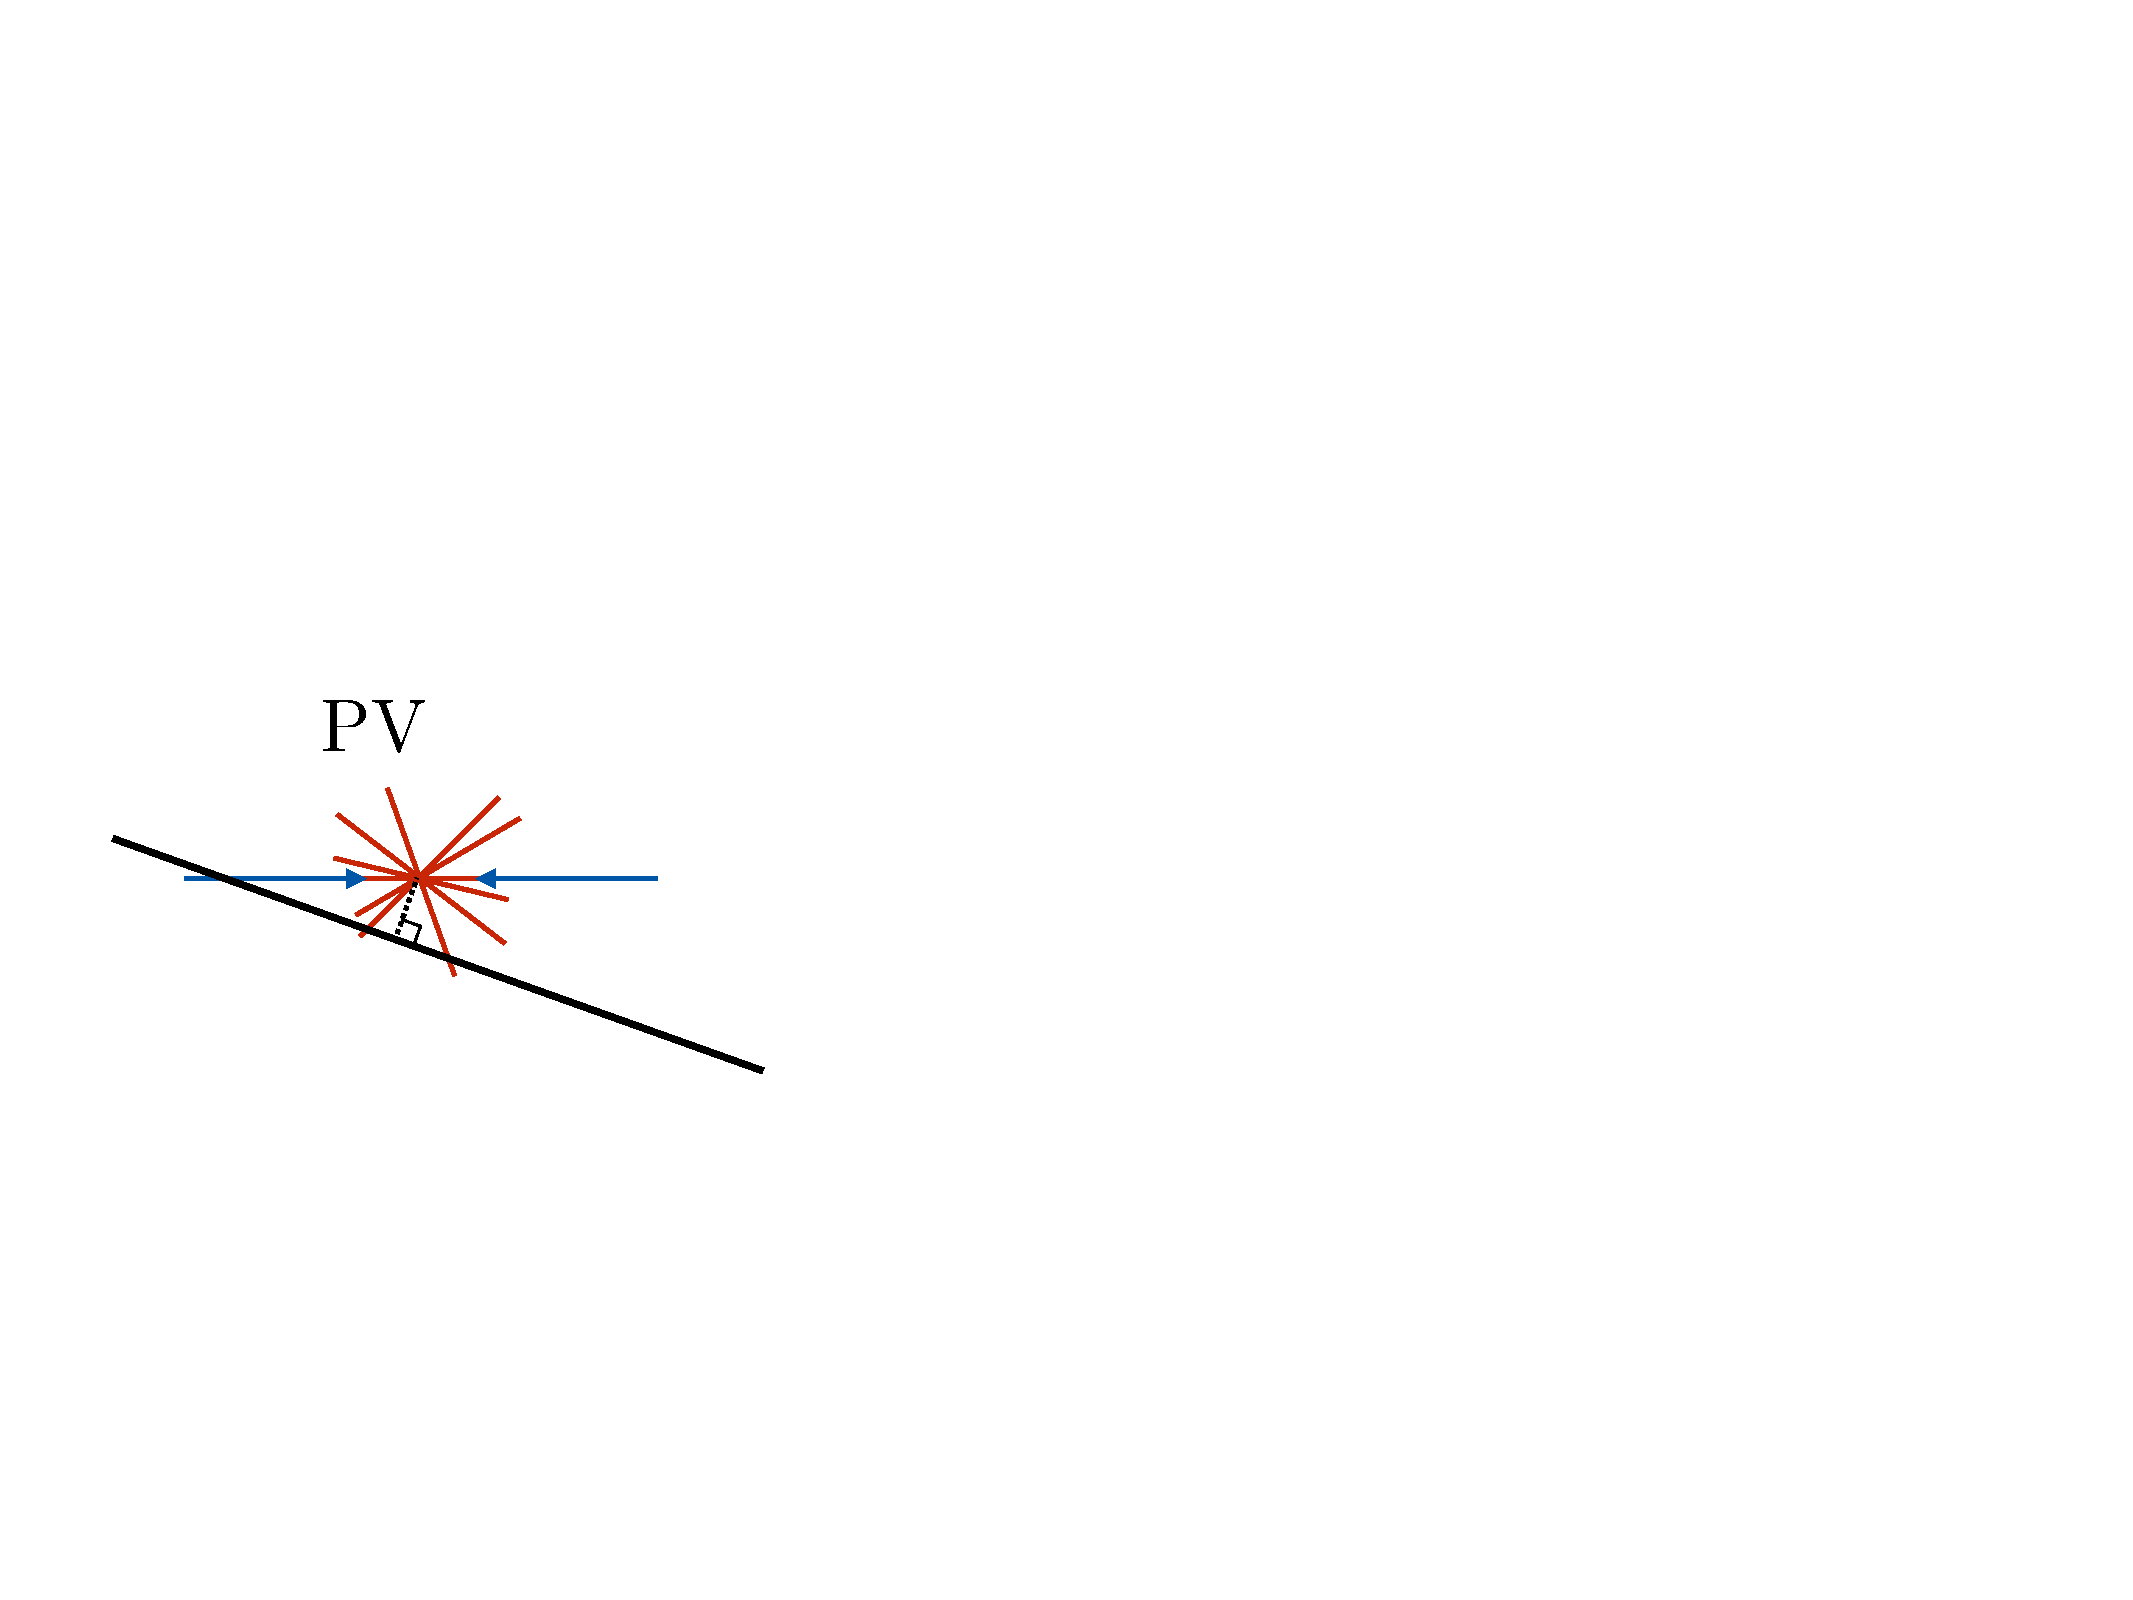
\includegraphics[width=0.4\textwidth]{figs/Selection/Impact_parameter.pdf}
    \caption{Impact parameter (dotted black line) between a track (black) and a vertex.}
    \label{fig:impact_parameter}   
\end{figure}
%%%%%%%%%%%%%%%%%%%%%%%%%%%%%%%%%%%%%%%%%%%%%%%%%%%%%%%%%%

\item \textbf{Impact parameter significance, $\chi^{2}_{\text{IP}}$:} The difference of a given vertex's $\chi^{2}/N_{\text{DOF}}$ with and without a specific track included in the fitting procedure.
\item \textbf{Flight distance significance, $\chi^{2}_{\text{FD}}$:} A measure of how significant the flight distance of a combination of particle is. This is defined as the $\chi^{2}$ associated with the difference in position of the two vertices, $\vec{\mathbf{d}} = \vec{\mathbf{v}}_2 - \vec{\mathbf{v}}_1$, where $\vec{\mathbf{v}}_1$ and $\vec{\mathbf{v}}_1$ are positions of the first and the second vertices. 
\item \textbf{Distance of closest approach, $\text{DOCA}(h,h')$:} The shortest distance between two tracks as shown in Fig~\ref{fig:doca}.
%%%%%%%%%%%%%%%%%%%%%%%%%%%%%%%%%%%%%%%%%%%%%%%%%%%%%%%%%%
\begin{figure}[!h]
    \centering
    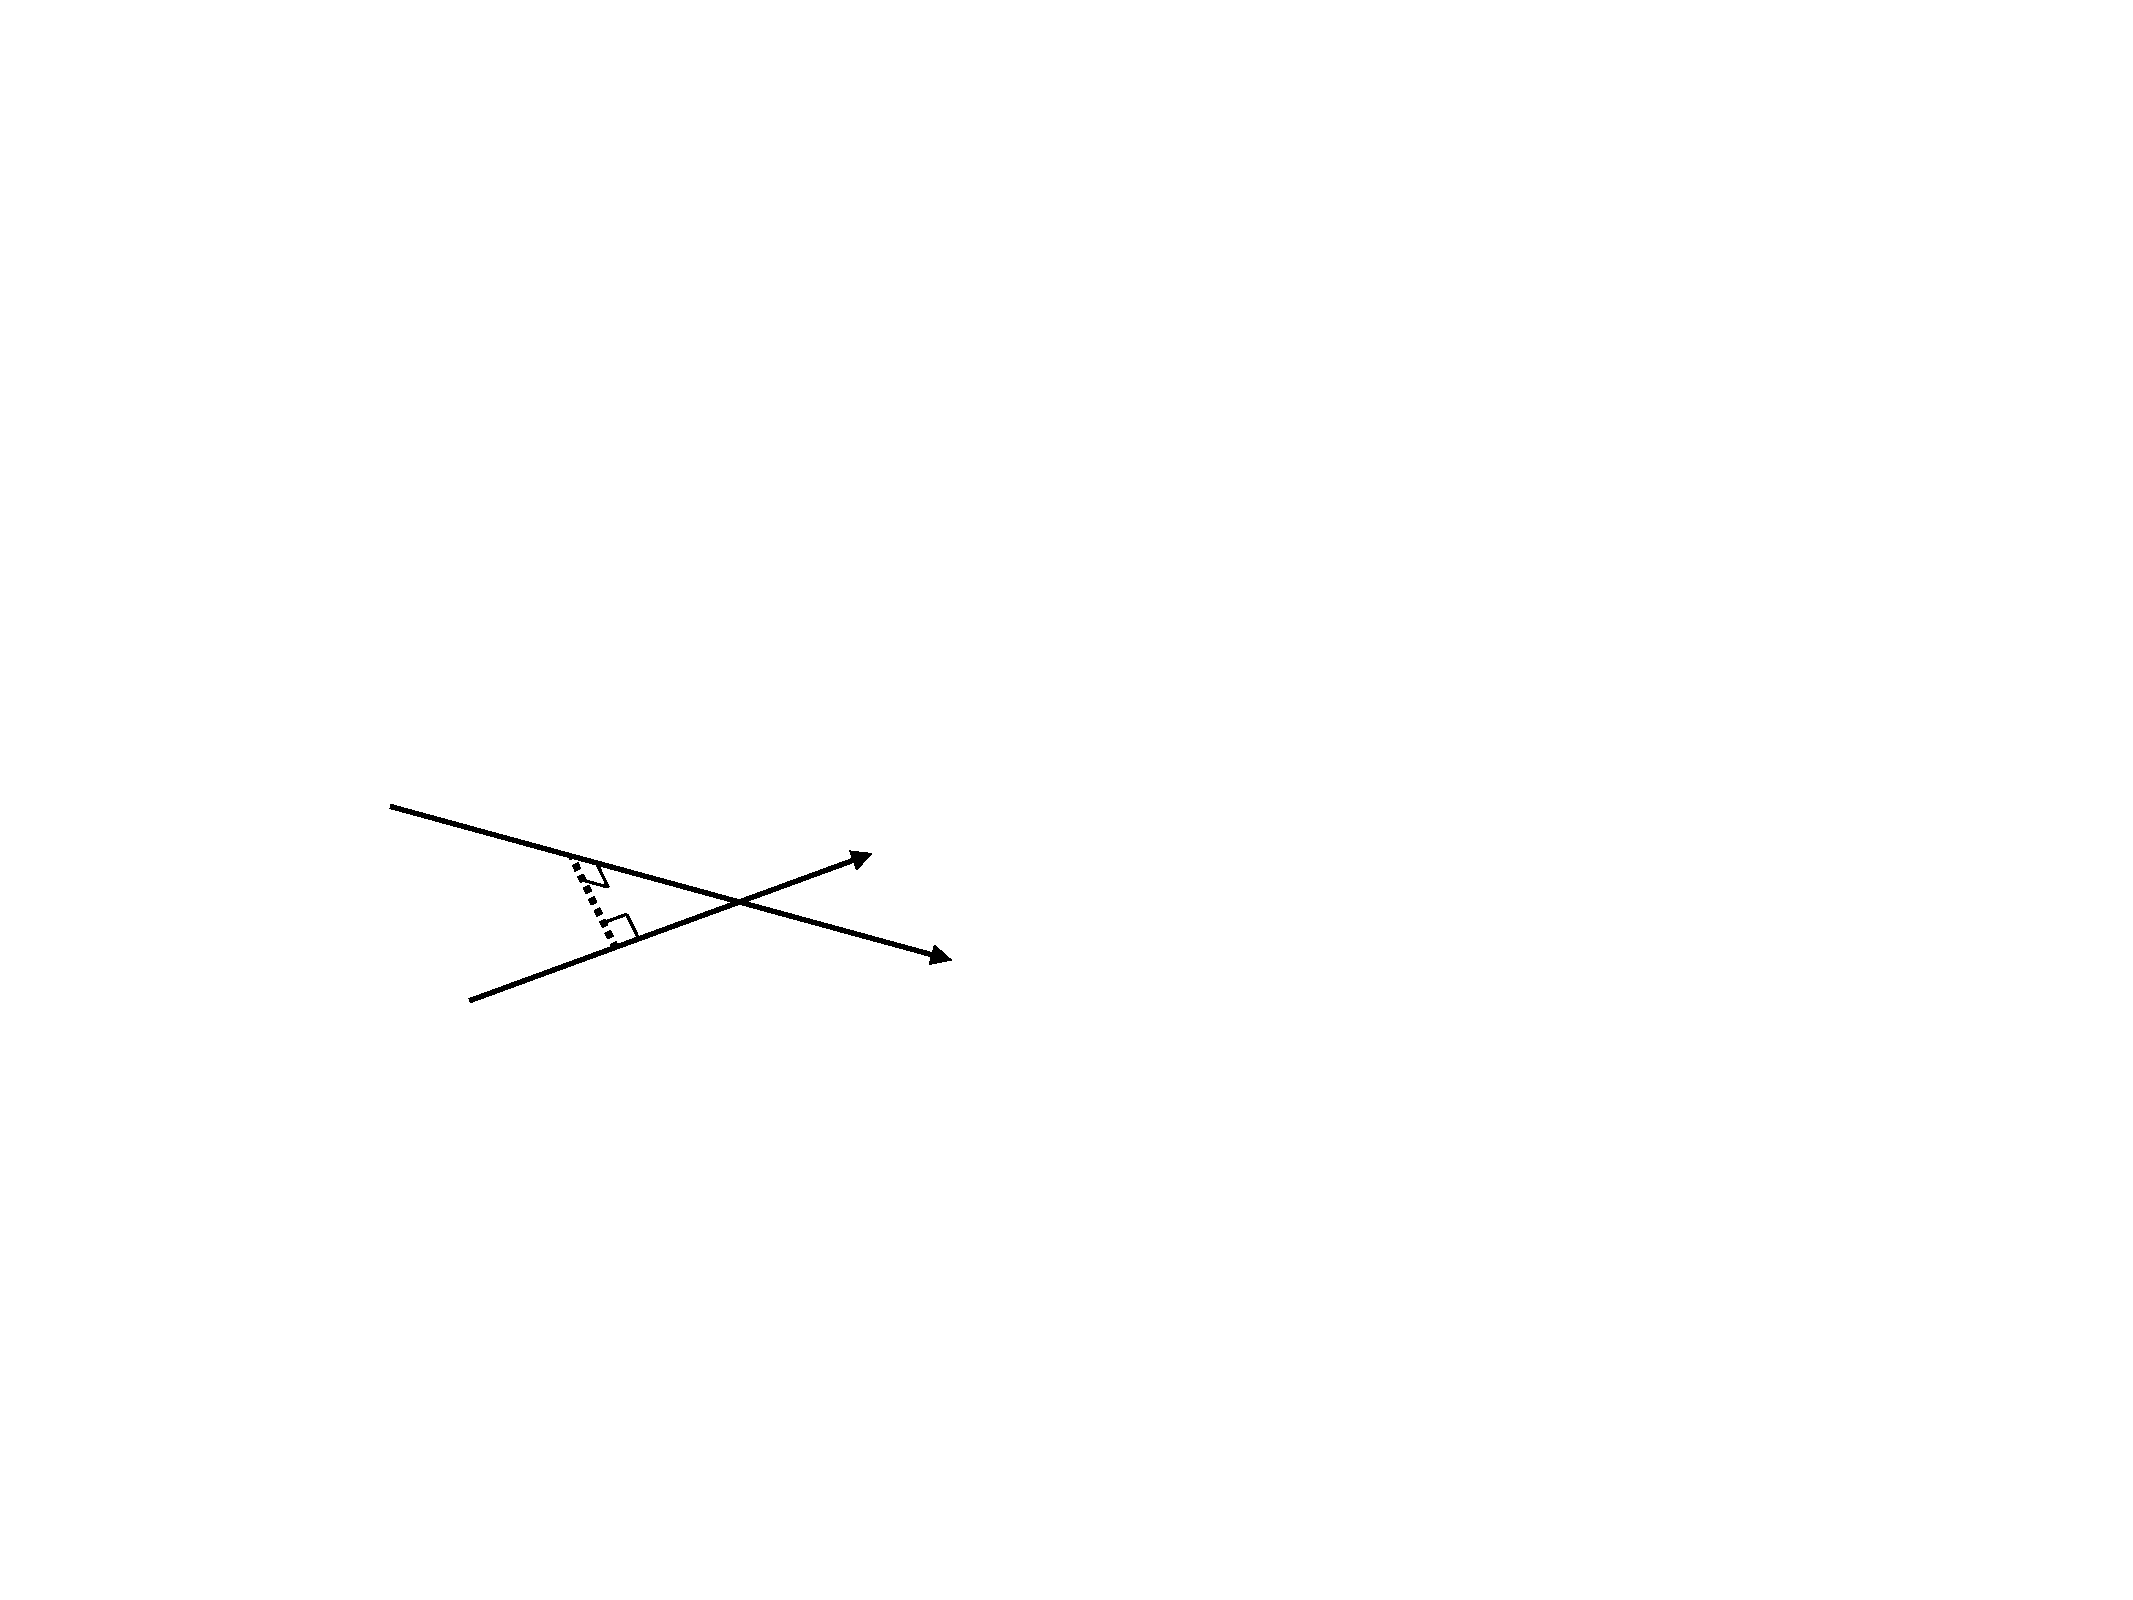
\includegraphics[width=0.4\textwidth]{figs/Selection/DOCA.pdf}
    \caption{Distance of closest approach (dotted black line) between two tracks.}
    \label{fig:doca}   
\end{figure}
%%%%%%%%%%%%%%%%%%%%%%%%%%%%%%%%%%%%%%%%%%%%%%%%%%%%%%%%%%


\item \textbf{Ghost track probability, $P_{\text{Ghost}}$:} This parameter quantifies the probability that a given track is an incorrect combination of tracking stations hits, known as a ghost track. The numerical value is the output of a Neural Network algorithm trained to separate true tracks from ghost tracks using simulated events. Various tracking parameters are inputs to the Neural Network including the number of hits in various tracking stations, the track fit quality and the number of tracks per event. 

\item \textbf{Direction angle:} The angle between a track's momentum vector and the vector connecting the primary vertex and decay vertex as shown in Fig.~\ref{fig:dira}.

%%%%%%%%%%%%%%%%%%%%%%%%%%%%%%%%%%%%%%%%%%%%%%%%%%%%%%%%%%
\begin{figure}[!h]
    \centering
    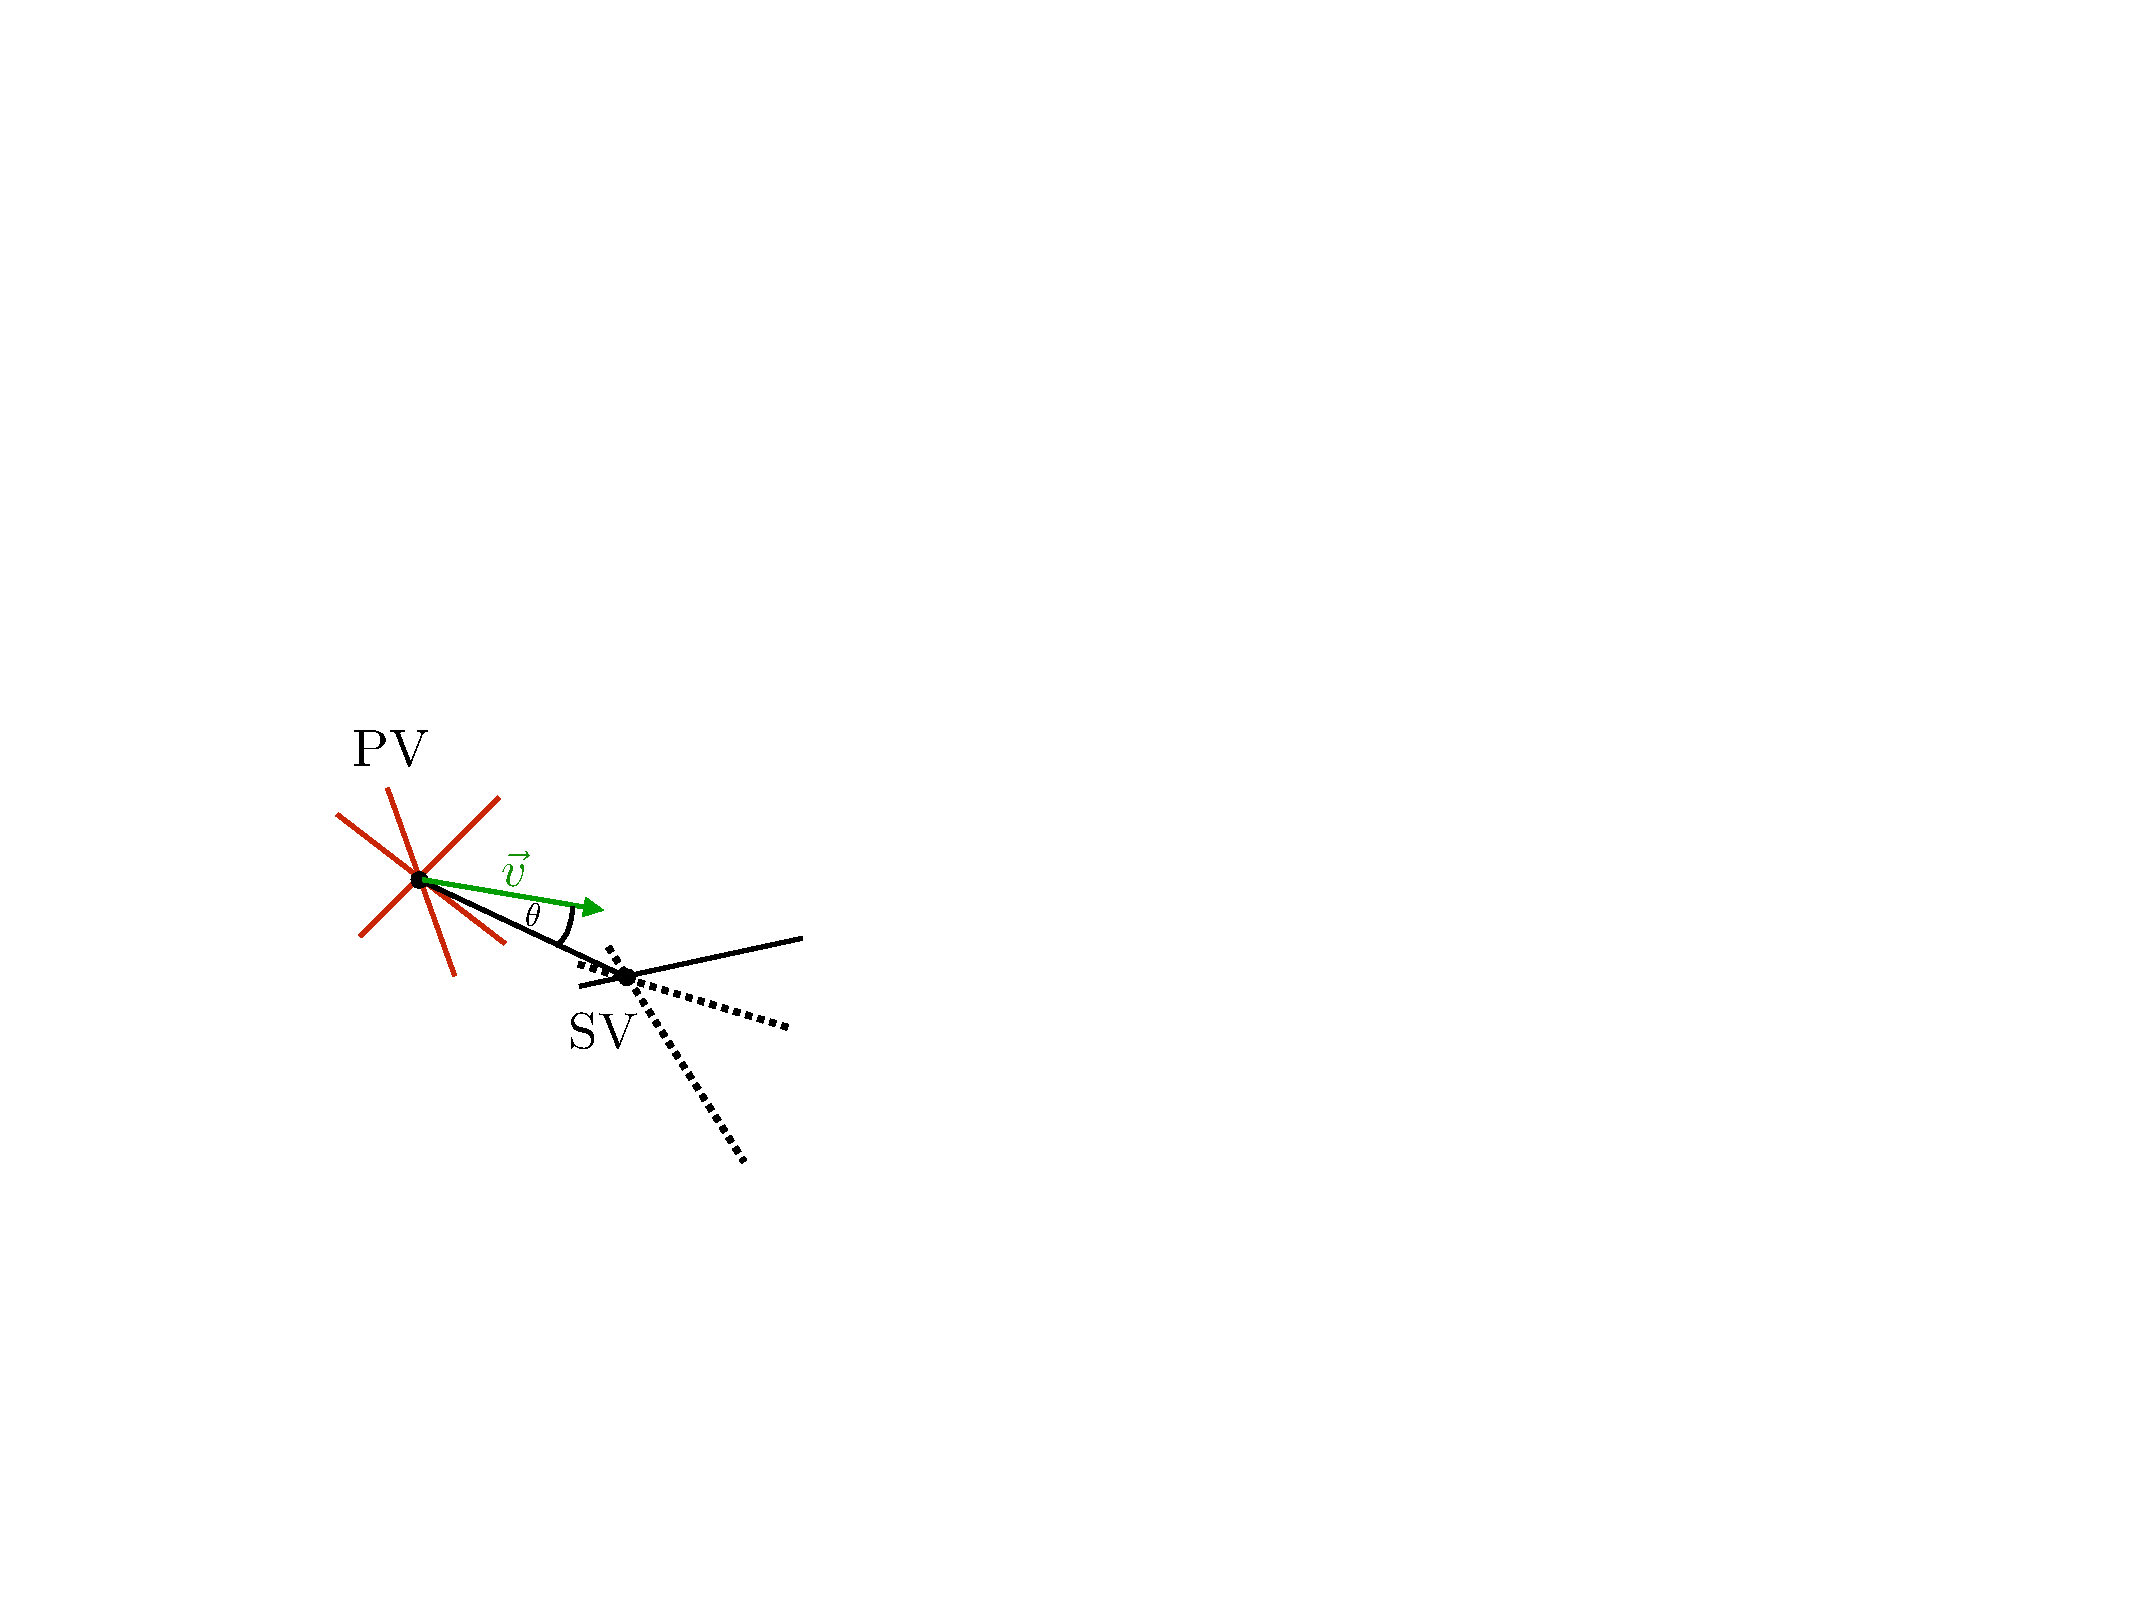
\includegraphics[width=0.4\textwidth]{figs/Selection/DIRA.pdf}
    \caption{Direction angle, $\theta$, between the line joining two vertices, primary vetex (PV) and secondary vertex (SV), and the momentum vector shown in green. The momentum vector corresponds to the momentum of the three tracks contributing to the SV. }
    \label{fig:dira}   
\end{figure}
%%%%%%%%%%%%%%%%%%%%%%%%%%%%%%%%%%%%%%%%%%%%%%%%%%%%%%%%%%


\item \textbf{Particle identification, $\text{PIDK}$:} The different in the log-likelihood of the kaon and pion hypothesis for a given track.  
\end{description}


As the final states are fully hadronic, the candidates are built from the combination of five tracks. Only \emph{long} tracks (those with hits in the \velo and tracking stations) are used to build these mesons. The track $\chi^{2}/N_{\text{DOF}}$ is required to be below $4.0$ to ensure these are well reconstructed. Additionally, they are required to have a total momentum $\ptot > 1000 \mevc$ and the transverse momentum is required to be $\pt > 100 \mevc$.
Due to the long lifetime and high boost of the \Bp and \D mesons, the decay products originate from a vertex that is displaced from the proton-proton collision vertex. In this case the trajectory of the \B or \D decay products do not pass through the primary collision position, as shown in Fig.~\ref{fig:impact_parameter}. A requirement is placed on the significance of the impact parameter between the track and the proton-proton collision vertex of $\chi^{2}_{\text{IP}} > 4$ to ensure all of the tracks used are inconsistent with originating at the primary interaction.  


Loose requirements are placed on \emph{Particle Identification} variables to ensure the tracks are of the required species. These are further tightened as detailed in Section~\ref{sec:pidrequirements}. Incorrect track candidates created by combining unrelated \velo and tracking station hits are suppressed by requiring the ghost track probability, $P_{\text{Ghost}}$, to be less than $0.4$. 

%%%%%% Ds/ D0 and phi construction

The tracks passing these requirements are combined in pairs or triplets to form the \Dsp and \phiz or \Dzb meson candidates.  
For the purpose of forming the \phiz candidates (or \Kp\Km pair), all combinations of two tracks are considered where the tracks are assigned the kaon mass. Only pairs which pass within $0.5\mm$ of one another at their closest point are retained. A number of requirements are imposed to ensure the pair are consistent with coming from a \phiz meson (or \Kp\Km pair) that originated in a \Bp meson decay. The vertex is required to be of good quality, the scalar sum of the transverse momentums must be greater than $1000\mevc$ and the flight distance significance is required to be $\chi^{2}_{\text{FD} } > 16$. Additionally the cosine of the direction angle, defined to be the angle between the momentum vector and flight vector, is required to be $\cos{\theta}>0$, preventing the vertex being backward of the PV when the momentum is in the forward direction. In the search for \decay{\Bp}{\Dsp\phiz} decays, the invariant mass of the two kaons is required to be within $150\mevcc$ of the known \phiz meson mass.  

The \Dzb meson candidates are selecting using a similar parameters, however the exact values of the cuts are changed to reflect the differences in properties of the \phiz and \Dzb mesons. The vertex quality and flight distance significance requirements are tightened to $\chi^{2}/N_{\text{DOF}} < 10$ and $\chi^{2}_{\text{FD} }  > 36$ respectively. Additionally, the scalar \pt sum requirment is increased to $\sum{|\pt|} > 1800 \mevc$ as the decay products tend to have higher transverse momentum. 


The \Dsp mesons candidates are created using combinations of three tracks given the mass hypotheses kaons or pions, depending on the decay mode being constructed. All combinations of three tracks are considered and only those in which all three tracks are within 0.5\mm of one another are retained. As with the \Dzb meson selection, the vertex quality, flight distance significance and scalar \pt sum requirements are $\chi^{2}/N_{\text{DOF}} < 10$, $\chi^{2}_{\text{FD} }  > 36$ and $\sum{|\pt|} > 1800 \mevc$ respectively.

%% B meson construction

The \Bp meson candidates are constructed from all possible combinations of the \Dsp and \phiz or \Dzb meson candidates in each event.
Requirements are placed on these combination to select just those consistent with \Bp mesons.
That is
\begin{itemize}
\item the combination is required to have a lifetime $\tau_{\Bp} > 0.2\ps$, 
\item the direction angle must pass the requirement $\cos{\theta}>0.999$,
\item the impact parameter significance is required to be $\chi^{2}_{\text{IP}} < 25$ to ensure the \Bp meson originated at the primary interaction, 
\item the vertex is required to have a quality of $\chi^{2}/N_{\text{DOF}} < 10$. 
\end{itemize}
%More requirements are additionally placed on the decay products that contribute to the \Bp meson. 
The selection requirements imposed on candidate \decay{\Bp}{\Dsp\phiz} and \decay{\Bp}{\Dsp\Kp\Km} decays in their respective \emph{Stripping Lines} are detailed in Table~\ref{tab:strippinglinecuts}. 


\begin{table}[!h]
\centering
\begin{tabular}{ l l l}
\hline
Particle       & Quantity                       & Requirement                       \\ 
\hline
\Bp            & Mass                           &  $4750 < m(\Dsp\phiz) < 7000\mevcc$    \\  
%               & Transverse Momentum            &  $\pt > 4000 \gevc$               \\  
               & Products \pt scalar sum        &  $\sum{|\pt|} > 5000 \mevc$         \\  
               & Vertex quality                 &  $\chi^{2}/N_{\text{DOF}} < 10$   \\  
               & Lifetime                       &  $\tau_{\Bp} > 0.2\ps$            \\  
               & Impact parameter significance  &  $\chi^{2}_{\text{IP}} < 25$      \\  
               & Direction angle                &  $\cos{\theta}>0.999$             \\  
               & \textit{$>$0 decay products with:}    &                                   \\
               & Momentum                       &  $\ptot > 10000 \mevc$            \\  
               & Transverse momentum            &  $\pt > 1700 \mevc$               \\  
               & Impact parameter significance  &  $\chi^{2}_{\text{IP}} > 16$      \\  
               & Impact parameter               &  $\text{IP} > 0.1\mm$             \\  
               & \textit{$>$1 decay products with:}   &                                   \\
               & Momentum                       &  $\ptot > 5000 \mevc$             \\  
               & Transverse momentum            &  $\pt > 500 \mevc$                \\
%               &                                &                                   \\
\hline  
\Dsp           & Mass                           &  $1770 < m(h^{+}h^{-}h^{+}) < 2068\mevcc$            \\  
               & Products \pt scalar sum        &  $\sum{|\pt|} > 1800 \mevc$         \\ 
               & Distance of closest approach   &  $\text{DOCA}(h^{+},h^{-}) < 0.5\mm$     \\
               & Distance of closest approach   &  $\text{DOCA}(h^{-},h'^{+}) < 0.5\mm$     \\    
               & Distance of closest approach   &  $\text{DOCA}(h^{+},h'^{+}) < 0.5\mm$     \\  
               & Direction angle                &  $\cos{\theta}>0$                 \\  
               & Vertex quality                 &  $\chi^{2}/N_{\text{DOF}} < 10$   \\   
               & Flight distance significance   &  $\chi^{2}_{\text{FD} }  > 36$    \\   
%               &                                &                                   \\  
% \hline
% \phiz          & Mass (only for \decay{\Bp}{\Dsp\phiz})&  $|m(\Kp\Km)-m_{\phiz}| < 150\mevcc$\\ 
%                & Products \pt scalar sum        &  $\sum{|\pt|} > 1000 \mevc$         \\  
%                & Distance of closest approach   &  $\text{DOCA}(\Kp,\Km) < 0.5\mm$  \\  
%                & Direction angle                &  $\cos{\theta}>0$                 \\  
%                & Vertex quality                 &  $\chi^{2}/N_{\text{DOF}} < 16$   \\   
%                & Flight distance significance   &  $\chi^{2}_{\text{FD} }  > 16$    \\   
%               &                                &                                   \\  
\hline
\phiz(\Dzb)    & Mass                           &  $870(1770) < m(X) < 1170(2068)\mevcc$\\ 
               & Products \pt scalar sum        &  $\sum{|\pt|} > 1000~(1800) \mevc$         \\  
               & Distance of closest approach   &  $\text{DOCA}(\Kp,\Km) < 0.5\mm$  \\  
               & Direction angle                &  $\cos{\theta}>0$                 \\  
               & Vertex quality                 &  $\chi^{2}/N_{\text{DOF}} < 16~(10)$   \\   
               & Flight distance significance   &  $\chi^{2}_{\text{FD} }  > 16~(36)$    \\   
%               &                                &                                   \\  
% \hline
% \Dzb           & Mass                           &  $1765 < m(h^{+}h^{-}h^{+}) < 1965\mevcc$\\  
%                & Products \pt scalar sum        &  $\sum{|\pt|} > 1800 \mevc$         \\  
%                & Distance of closest approach   &  $\text{DOCA}(\Kp,\Km) < 0.5\mm$  \\  
%                & Direction angle                &  $\cos{\theta}>0$                 \\  
%                & Vertex quality                 &  $\chi^{2}/N_{\text{DOF}} < 10$   \\   
%                & Flight distance significance   &  $\chi^{2}_{\text{FD} }  > 36$    \\
\hline
\Kpm(\pipm)    & Track quality                  &  $\chi^{2}/N_{\text{DOF}}<4.0$    \\  
               & Transverse momentum            &  $\pt > 100 \mevc$                \\  
               & Momentum                       &  $\ptot > 1000 \mevc$             \\  
               & Impact parameter significance  &  $\chi^{2}_{\text{IP}} > 4$       \\  
               & Ghost track probability        &  $P_{\text{Ghost}} < 0.4$         \\
               & Particle identification        &  $\text{PIDK}>-10$ ($\text{PIDK}<20$)\\  
\hline
\end{tabular}
\caption{Selection requirements for \decay{\Bp}{\Dsp\phiz}, \decay{\Bp}{\Dsp\Kp\Km} and \decay{\Bp}{\Dsp\Dzb} candidates. The \phiz meson invariant mass window is not applied to \decay{\Bp}{\Dsp\Kp\Km} candidates.}
\label{tab:strippinglinecuts}
\end{table}

%%%%%%%%%%%%%%%%%%%%%% DONE %%%%%%%%%%%%%%%%%%%%%%
%B CombCut
%(
% ASUM(
%       SUMTREE(
%                PT,(
%                      ISBASIC | 
%                      (ID=='gamma')
%                   )
%                ,0.0
%             )
%       )>5000*MeV) & 
% (AM<7000*MeV) & 
% (AM>4750*MeV)

% B MotherCut

% (VFASPF(VCHI2/VDOF)<10) &
%(BPVLTIME()>0.2*ps) & 
%(BPVIPCHI2()<25) & 
%(BPVDIRA>0.999)
% (INTREE(
%          HASTRACK & 
%          (P>10000*MeV) & 
%          (PT>1700*MeV) & 
%          (TRCHI2DOF<4.) & 
%          (MIPCHI2DV(PRIMARY)>16) & 
%          (MIPDV(PRIMARY)>0.1*mm) )) & 
% (NINTREE(
%          (
%             ISBASIC & 
%             HASTRACK & 
%             (TRCHI2DOF<4.) & 
%             (PT > 500*MeV) & 
%             (P > 5000*MeV)
%          ) > 1
% )


%X2PiPi
%(ASUM(PT)>1000*MeV) & 
% (AM < 5.2*GeV) & 
% (AHASCHILD(
%             (
%                ISBASIC & 
%                HASTRACK & 
%                (TRCHI2DOF<4.) & 
%                (PT > 500*MeV) & 
%                (P > 5000*MeV)
%             )
%          )
% ) & 
% (ADOCA(1,2)<0.5*mm)

%ADMASS('phi(1020)') < 150*MeV

%PiInput
%(TRCHI2DOF<4.0) & 
% (PT>100*MeV) & 
% (P>1000*MeV) & 
% (MIPCHI2DV(PRIMARY)>4.0) & 
% (TRGHP<0.4)


%D2HHHFilter
%
% (NINGENERATION(
%                ('p+'==ABSID) & 
%                (PIDp < -10),1
%                ) == 0
% ) & 
% (NINGENERATION(   
%                ('K+'==ABSID) & 
%                (PIDK < -10)
%                , 1) == 0
% ) & 
% (NINGENERATION(
%                ('pi+'==ABSID) & 
%                (PIDK > 20)
%                , 1) == 0
% )

% D2HHH CombCut
% (ASUM(PT)>1800*MeV) & 
% (in_range(1769.62*MeV,AWM('K+','K+','pi-'),2068.49*MeV)) & 
% (AHASCHILD(
              
%             ISBASIC & 
%             HASTRACK & 
%             (TRCHI2DOF<4.) & 
%             (PT > 500*MeV) & 
%             (P > 5000*MeV)          
%          )
% ) & 
% (ADOCA(1,3)<0.5*mm) & 
% (ADOCA(2,3)<0.5*mm)

% D2HHH MotherCut
% (VFASPF(VCHI2/VDOF)<10) & 
% (BPVVDCHI2>36) & 
% (BPVDIRA>0)

% PhiMotherCut
% (VFASPF(VCHI2/VDOF)<16) & 
% (BPVVDCHI2>16) & 
% (BPVDIRA>0)


%%%%%%%%%%%%%%%%%%%%%%%%%%%%%%%%%%%%%%%%%%%%%%%%%


%HHPionsInput
%(PT>100*MeV) & (P>2000*MeV)


Two slightly different strategies are used for the normalisation channel selection in the search for \decay{\Bp}{\Dsp\phiz} and \decay{\Bp}{\Dsp\Kp\Km} events.
In the former, a dedicated \decay{\Bp}{\Dsp\Dzb} \emph{Stripping Line} is used to reconstruct the normalisation channel decays.
The \emph{Stripping Line} selection for this line is listed in Table~\ref{tab:strippinglinecuts}.

% \begin{table}[h]
%    \centering
%       \begin{tabular}{l l}
%          \hline
%          Mode & Stripping line \\ 
%          \hline
%          \decay{\Bp}{\Dsp\phiz}        & \texttt{StrippingB2DPhiD2HHHPIDBeauty2CharmLine}    \\
%          \decay{\Bp}{\Dsp\Kp\Km}       & \texttt{StrippingB2DKKD2HHHCFPIDBeauty2CharmLine}   \\
%          \decay{\Bp}{\Dsp\Dzb}         & \texttt{StrippingB2D0DBeauty2CharmLine}             \\
%          \hline
%       \end{tabular}
%    
%    \caption{\emph{Stripping Lines} used in this analysis.}
%    \label{tab:strippinglines}
% \end{table}

The \emph{Stripping Line} used in the search for \decay{\Bp}{\Dsp\Kp\Km} decays covers the full $m(\Kp\Km)$ phase-space. This includes the \Dzb mass such that this line reconstructs both the signal and normalisation channels simultaneously. 
Both modes are selected using this line to reduce systematic uncertainty in the ratio of selection efficiencies.

% \begin{table}[h]
% \centering
% \begin{tabular}{ l l l}
% \hline
% Particles      & Quantity                       & Requirement                       \\ 
% \hline
% \Bp            & Mass                           &  $4750 < m(\Dsp\Dzb) < 7000\mevcc$    \\ 
%                & Products \pt scalar sum        &  $\sum{|\pt|} > 5000 \mevc$         \\  
%                & Vertex quality                 &  $\chi^{2}/N_{\text{DOF}} < 10$   \\  
%                & Lifetime                       &  $\tau_{\Bp} > 0.2\ps$            \\  
%                & Impact parameter significance  &  $\chi^{2}_{\text{IP}} < 25$      \\  
%                & Direction angle                &  $\cos{\theta}>0.999$             \\  
%                & \textit{$>$0 decay products with:}    &                                   \\
%                & Momentum                       &  $\ptot > 10000 \mevc$            \\  
%                & Transverse momentum            &  $\pt > 1700 \mevc$               \\  
%                & Impact parameter significance  &  $\chi^{2}_{\text{IP}} > 16$      \\  
%                & Impact parameter               &  $\text{IP} > 0.1\mm$             \\  
%                & \textit{$>$1 decay products with:}   &                                   \\
%                & Momentum                       &  $\ptot > 5000 \mevc$             \\  
%                & Transverse momentum            &  $\pt > 500 \mevc$                \\
% %               &                                &                                   \\  
% \hline
% \Dsp           & Mass                           &  $1770 < m(h^{+}h^{-}h^{+}) < 2068\mevcc$            \\  
%                & Products \pt scalar sum        &  $\sum{|\pt|} > 1800 \mevc$         \\ 
%                & Distance of closest approach   &  $\text{DOCA}(h^{+},h^{-}) < 0.5\mm$     \\
%                & Distance of closest approach   &  $\text{DOCA}(h^{-},h'^{+}) < 0.5\mm$     \\    
%                & Distance of closest approach   &  $\text{DOCA}(h^{+},h'^{+}) < 0.5\mm$     \\   
%                & Direction angle                &  $\cos{\theta}>0$                 \\  
%                & Vertex quality                 &  $\chi^{2}/N_{\text{DOF}} < 10$   \\   
%                & Flight distance significance   &  $\chi^{2}_{\text{FD} }  > 36$    \\   
% %               &                                &                                   \\  
% \hline
% \Dzb           & Mass                           &  $1765 < m(h^{+}h^{-}h^{+}) < 1965\mevcc$\\  
%                & Products \pt scalar sum        &  $\sum{|\pt|} > 1800 \mevc$         \\  
%                & Distance of closest approach   &  $\text{DOCA}(\Kp,\Km) < 0.5\mm$  \\  
%                & Direction angle                &  $\cos{\theta}>0$                 \\  
%                & Vertex quality                 &  $\chi^{2}/N_{\text{DOF}} < 10$   \\   
%                & Flight distance significance   &  $\chi^{2}_{\text{FD} }  > 36$    \\   
% %               &                                &                                   \\  
% \hline
% \Kpm (\pipm)   & Track quality                  &  $\chi^{2}/N_{\text{DOF}}<4.0$    \\  
%                & Transverse momentum            &  $\pt > 100 \mevc$                \\  
%                & Momentum                       &  $\ptot > 1000 \mevc$             \\  
%                & Impact parameter significance  &  $\chi^{2}_{\text{IP}} > 4$       \\  
%                & Ghost track probability        &  $P_{\text{Ghost}} < 0.4$         \\
%                & Particle identification        &  $\text{PIDK}>-10$ ($\text{PIDK}<20$)\\
% \hline
% \end{tabular}
% 
% \caption{Selection requirements for \decay{\Bp}{\Dsp\Dzb} candidates.}

% \label{tab:strippinglinecuts}
% \end{table}



% D2KKPi Mother
% (VFASPF(VCHI2/VDOF)<10) & (BPVVDCHI2>36) & (BPVDIRA>0)



% D2KKPi Comb12 
% (ADOCA(1,2)<0.5*mm)


% D2KKPi Comb
% 
% (ASUM(PT)>1800*MeV) & 
% (in_range(1769.62*MeV,AWM('K-','K-','pi+'),2068.49*MeV)) & 
% (AHASCHILD(
%             ISBASIC & 
%             HASTRACK & 
%             (TRCHI2DOF<4.) & 
%             (PT > 500*MeV) & 
%             (P > 5000*MeV)  
%          )  
% ) & 
% (ADOCA(1,3)<0.5*mm) & 
% (ADOCA(2,3)<0.5*mm)



% K input 
% (TRCHI2DOF<4.0) & (PT>100*MeV) & (P>1000*MeV) & (MIPCHI2DV(PRIMARY)>4.0) & (TRGHP<0.4)


% D2KK Mother
% 
% (VFASPF(VCHI2/VDOF)<10) & 
% (BPVVDCHI2>36) & 
% (BPVDIRA>0)




% D2KK Comb
% 
% (ASUM(PT)>1800*MeV) & 
% (in_range(1764.84*MeV,AWM('K+','K-'),1964.84*MeV)) & 
% (AHASCHILD(
%          ISBASIC & 
%          HASTRACK & 
%          (TRCHI2DOF<4.) & 
%          (PT > 500*MeV) & 
%          (P > 5000*MeV)    
%       )
% ) & 
% (ADOCA(1,2)<0.5*mm)

% D2HH
% (NINGENERATION(('p+'==ABSID) & (PIDp < -10),1) == 0) & (NINGENERATION(('K+'==ABSID) & (PIDK < -10), 1) == 0) & (NINGENERATION(('pi+'==ABSID) & (PIDK > 20), 1) == 0)


% B mother cut
% (VFASPF(VCHI2/VDOF)<10) & 
% (
%    INTREE(HASTRACK & 
%    (P>10000*MeV) & 
%    (PT>1700*MeV) & 
%    (TRCHI2DOF<4.) & 
%    (MIPCHI2DV(PRIMARY)>16) & 
%    (MIPDV(PRIMARY)>0.1*mm))
% ) & 
% (
%    NINTREE( 
%             ISBASIC & 
%             HASTRACK & 
%             (TRCHI2DOF<4.) & 
%             (PT > 500*MeV) & 
%             (P > 5000*MeV)     
%          ) > 1
% ) & 
% (BPVLTIME()>0.2*ps) & 
% (BPVIPCHI2()<25) & 
% (BPVDIRA>0.999)


% B comb
% (ASUM(
%    SUMTREE(PT,ISBASIC,0.0) )>5000*MeV
% ) & 
% (AM<7000*MeV) & 
% (AM>4750*MeV)

%%%%%%%%%%%%% done %%%%%%%%%%%


%\clearpage


\subsection{Particle identification requirements}
\label{sec:pidrequirements}
%Particle identification variables help to determine the species of tracks passing though the \lhcb detector. Using information from the RICH sub-detectors, the likelihood of different mass hypotheses are compared to the pion hypothesis. Loose 
Requirements are made on the kaon hypothesis PID variable to reduce the contribution from other types of hadrons and background from other \bquark-hadron decays with misidentified hadrons. 
The parameter is defined to be
\begin{equation}
\text{PIDK} = \Delta \log(K - \pi) = \log\mathcal{L}(K) - \log\mathcal{L}(\pi)
\end{equation}
where $\mathcal{L}(K)$ and $\mathcal{L}(\pi)$ are the likelihoods of the kaon and pion hypotheses respectively.
The requirements placed on each decay product are listed in Table~\ref{tab:selection_pid_cuts}.

\begin{table}[h]
   \centering
      \begin{tabular}{l l l}
         \hline
         Decay mode & Species & PID requirement\\ 
         \hline
         \decay{\phiz}{\Kp\Km}      & \Kp    & $\text{PIDK} > 0$  \\
                                    & \Km    & $\text{PIDK} > 0$  \\
         \hline
         \decay{\Dzb}{\Kp\Km}       & \Kp    & $\text{PIDK} > 0$  \\
                                    & \Km    & $\text{PIDK} > 0$  \\
         \hline
         \decay{\Dsp}{\Kp\Km\pip}   & \Kp    & $\text{PIDK} > -5$ \\
                                    & \Km    & $\text{PIDK} > -5$ \\
                                    & \pip   & $\text{PIDK} < 5$  \\
         \hline
         \decay{\Dsp}{\pip\pim\pip} & \pip   & $\text{PIDK} < 5$  \\
                                    & \pim   & $\text{PIDK} < 5$  \\
                                    & \pip   & $\text{PIDK} < 5$  \\
         \hline
         \decay{\Dsp}{\Kp\pim\pip}  & \Kp    & $\text{PIDK} > -5$ \\
                                    & \pim   & $\text{PIDK} < 5$  \\
                                    & \pip   & $\text{PIDK} < 5$  \\
         \hline
      \end{tabular}
   \caption{Particle identification requirements applied to kaons and pions.}
   \label{tab:selection_pid_cuts}
\end{table}

The distribution of PIDK for pions and kaons is shown in Fig.~\ref{fig:selection_PIDK_distribution} as determined from data calibration samples.
%%%%%%%%%%%%%%%%%%%%%%%%%%%%%%%%%%%%%%%%%%%%%%%%%%%%%%%%%%
\begin{figure}[!h]
    \centering
        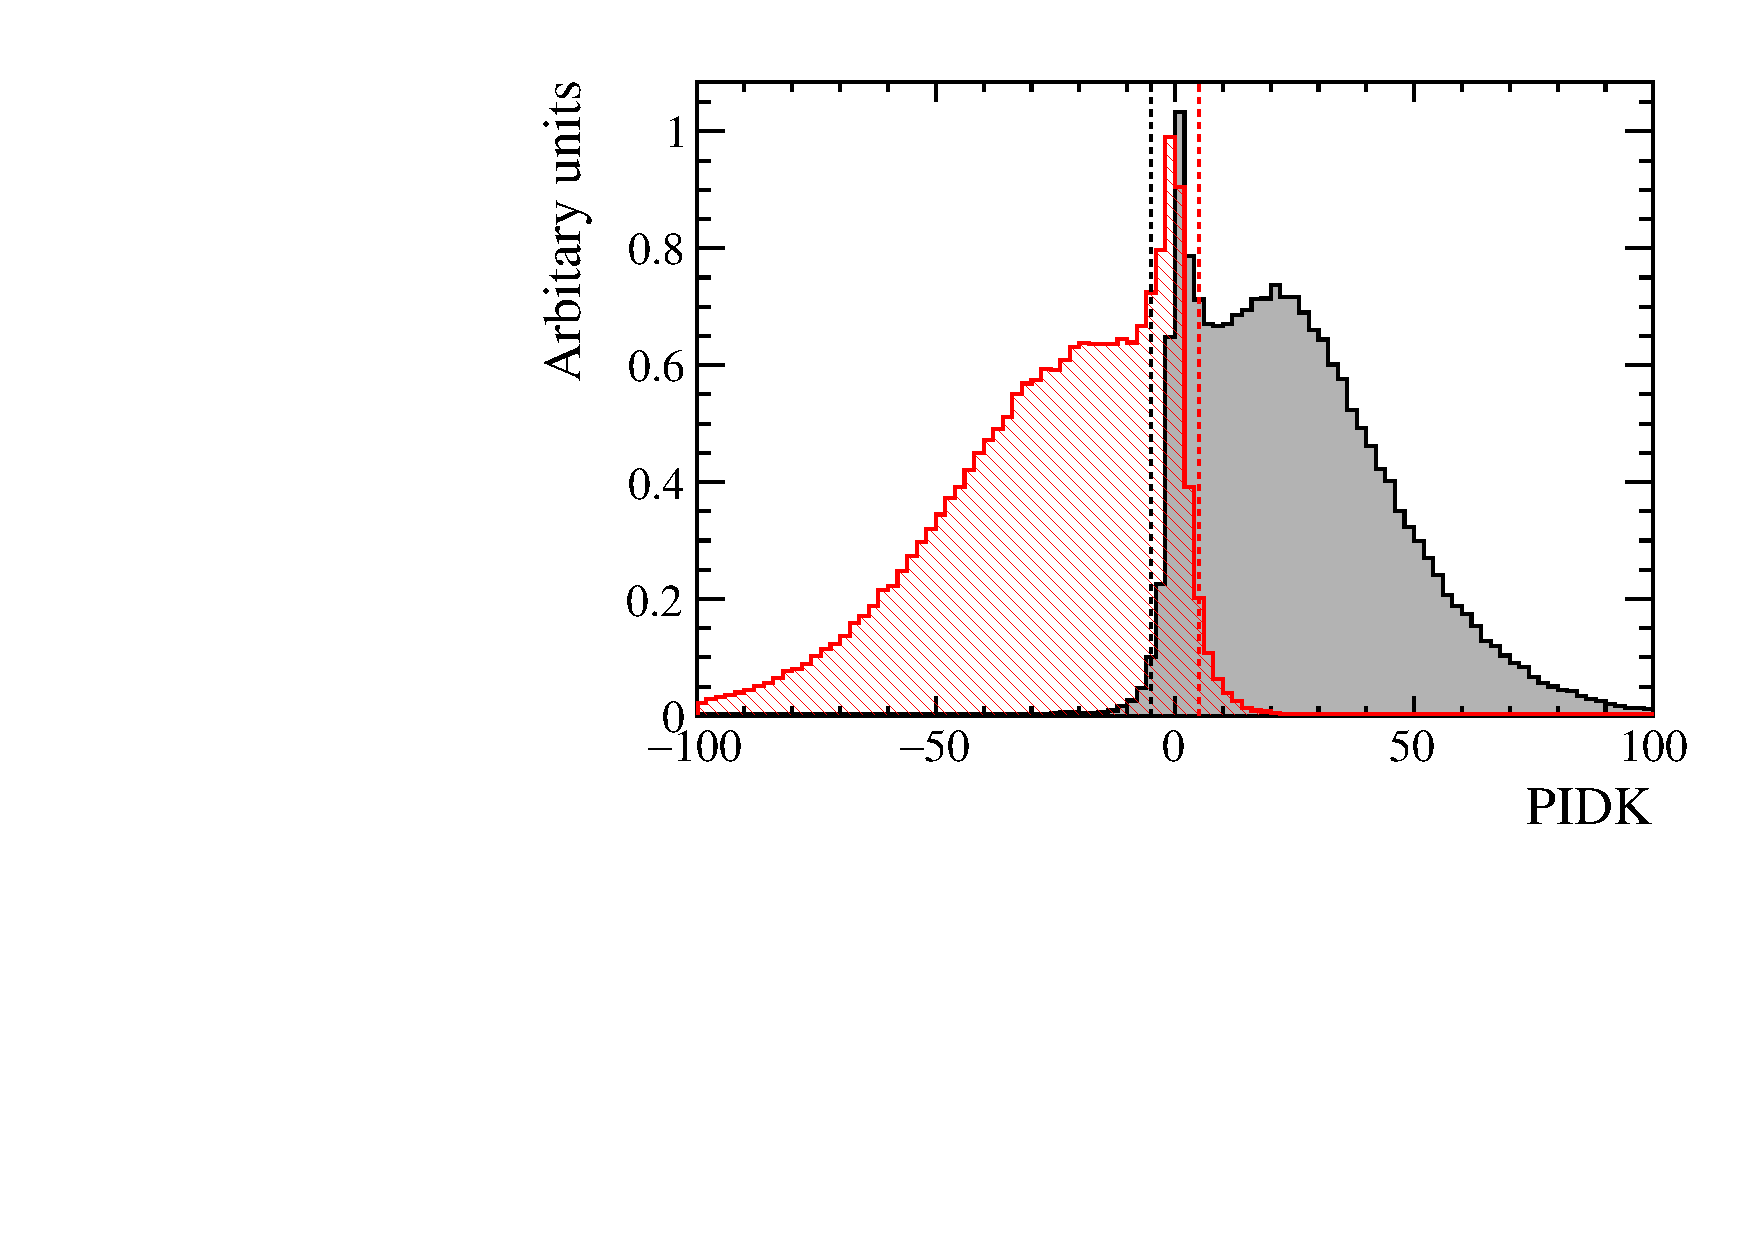
\includegraphics[width=0.6\textwidth]{figs/Selection/Calib_sample_PIDK.pdf}
        \caption{The distribution of the particle identification variable PIDK for pions (red) and kaons (black) from data calibration samples. The vertical dashed lines illustrate the requirements $\text{PIDK}>5$ and $\text{PIDK}<-5$ applied to kaons and pions respectively.}
    \label{fig:selection_PIDK_distribution}   
\end{figure}
%%%%%%%%%%%%%%%%%%%%%%%%%%%%%%%%%%%%%%%%%%%%%%%%%%%%%%%%%%





\subsection{Charmless and single-charm backgrounds}


Decays of \Bp mesons that didn't proceed via \D mesons could form a peaking background below the signal invariant mass distributions when they decay to the same final state.
The signal mode could receive contributions from the decays $\decay{\Bp}{h^{+}h^{-}h^{+}\phiz}$ or $\decay{\Bp}{h^{+}h^{-}h^{+}h^{+}h^{-}}$, referred to as charmless backgrounds. Here $h^{\pm}$ is used to represent \Kpm or \pipm in the specific \Dsp, \Dzb or \phiz final state.
The normalisation mode is also susceptible, however as it involves two charm mesons it could receive contributions from the decays $\decay{\Bp}{h^{+}h^{-}h^{+}\Dzb}$ or $\decay{\Bp}{\Dsp h^{+}h^{-}}$, referred to as single-charm backgrounds, and $\decay{\Bp}{h^{+}h^{-}h^{+} h^{+}h^{-}}$ referred to as a charmless background.
These backgrounds can be suppressed by requiring the \D meson decay vertex to be displaced from the \Bp meson decay vertex. Requirements are applied to the significance of the vertex separation ($\chi^{2}_{\text{FD}}$).

The residual yields of charmless backgrounds in the signal mode are estimated by performing a fit to the \Bp invariant mass for candidates with $25 < |m(h^{+}h^{-}h^{+}) - m(\Dsp)| < 50\mevcc $. This background estimation is performed separately for the \decay{\Bp}{\Dsp\phiz} and \decay{\Bp}{\Dsp\Kp\Km} searches. 

For the \decay{\Bp}{\Dsp\Dzb} normalisation channel, a two-dimensional optimisation is performed to calculate the contribution from decays without a \Dsp meson, \Dzb meson or both. 
The two-dimensional space defined by the \Dsp and \Dzb masses is split into four types of area as shown in Fig~\ref{fig:2d_normalisation}.

%%%%%%%%%%%%%%%%%%%%%%%%%%%%%%%%%%%%%%%%%%%%%%%%%%%%%%%%%%
\begin{figure}[!h]
    \centering
        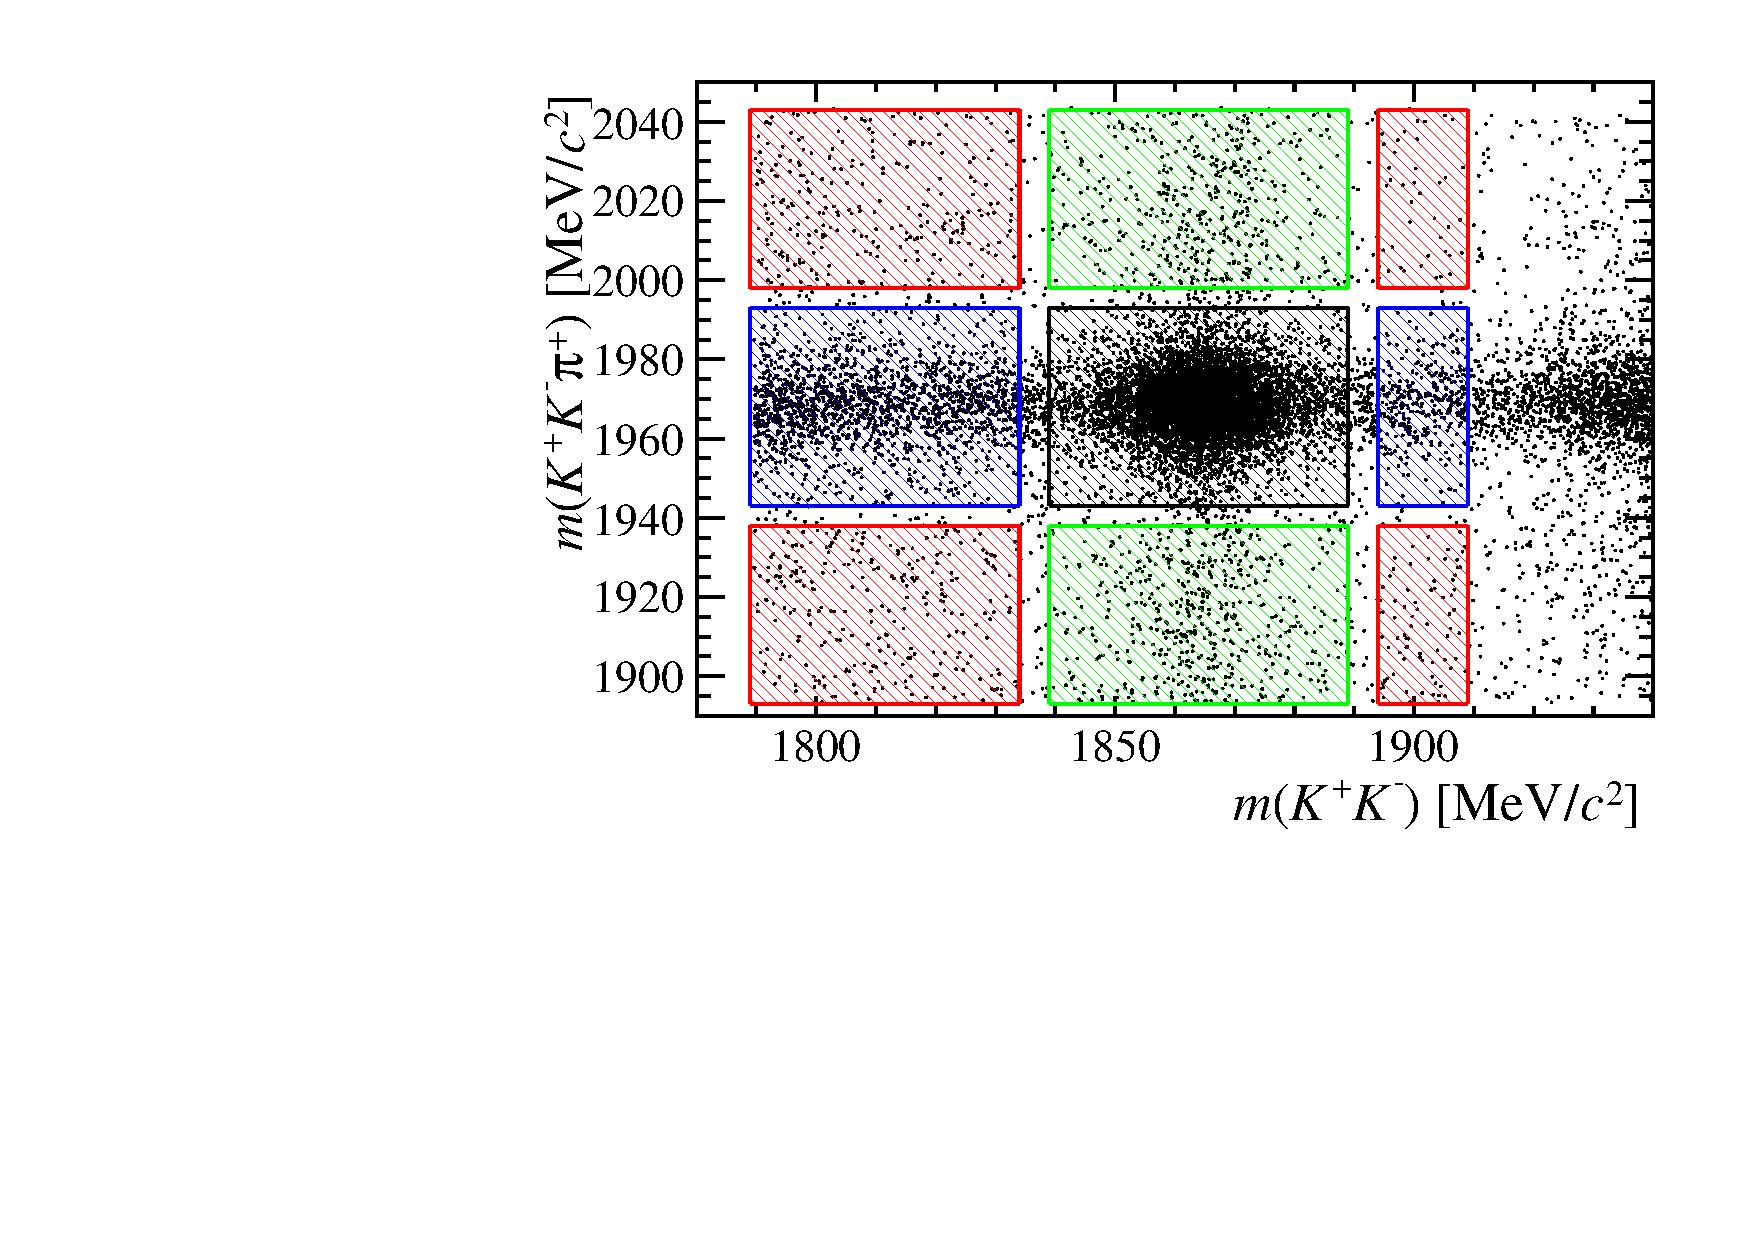
\includegraphics[width=0.6\textwidth]{figs/Selection/B2DsD0_2D_mass_Ds2KKPiRun2.pdf}
        \caption{Candidate \decay{\Bp}{\Dsp\Dzb} decays plotted as a function of the \Dsp and \Dzb invariant mass. The four regions described in the text are highlighted.}
    \label{fig:2d_normalisation}   
\end{figure}
%%%%%%%%%%%%%%%%%%%%%%%%%%%%%%%%%%%%%%%%%%%%%%%%%%%%%%%%%%

\begin{enumerate}
\item Areas in which only $\decay{\Bp}{h^{+}h^{-}h^{+}h^{+}h^{-}}$ decays contribute (red).
\item Areas in which either $\decay{\Bp}{D_{s}^{+}h^{+}h^{-}}$  or $\decay{\Bp}{h^{+}h^{-}h^{+} h^{+}h^{-}}$ decays can contribute (blue). 

\item Areas in which either $\decay{\Bp}{h^{+}h^{-}h^{+}\Dzb}$ or $\decay{\Bp}{h^{+}h^{-}h^{+} h^{+}h^{-}}$ decays can contribute (green). 
\item The signal region in which $\decay{\Bp}{D_{s}^{+} \Dzb}$, $\decay{\Bp}{h^{+}h^{-}h^{+}\Dzb}$, $\decay{\Bp}{D_{s}^{+}h^{+}h^{-}}$ or $\decay{\Bp}{h^{+}h^{-}h^{+}h^{+}h^{-}}$ decays could contribute (black).
\end{enumerate}   

Asymmetric \Dzb sidebands are used to prevent misidentified \decay{\Bp}{\Dsp (\decay{\Dzb}{\Km\pip})} decays from being included in the sideband sample.
The optimal selection requirements are chosen such that the maximal signal efficiency is achieved for a residual charmless contribution of $<2\%$ of the normalisation yield.

The optimisation of the signal and normalisation cuts is performed separately for each different \Dsp decay mode, and for the \decay{\Bp}{\Dsp\Kp\Km} and \decay{\Bp}{\Dsp\phiz} selections. The optimised requirements are listed in Table~\ref{tab:selection_fd_cuts}, along with the estimated residual yields of charmless and single charm yields in the signal region.  


\begin{table}[h]
   \centering
      \begin{tabular}{l c c c c }
         \hline
         \Bp decay mode         & \Dsp decay mode             & $\chi^{2}_{\text{FD}}(\Dsp)$  & $\chi^{2}_{\text{FD}}(\Dzb)$  & Residual yields \\ 
         \hline
         \decay{\Bp}{\Dsp\phiz} & \decay{\Dsp}{\Kp\Km\pip}    &  0.0              & -                 & 0.0             \\
         \decay{\Bp}{\Dsp\phiz} & \decay{\Dsp}{\Kp\pim\pip}   &  25.0             & -                 & 2.6             \\
         \decay{\Bp}{\Dsp\phiz} & \decay{\Dsp}{\pip\pim\pip}  &  5.0              & -                 & 0.0             \\
         \decay{\Bp}{\Dsp\Dzb}  & \decay{\Dsp}{\Kp\Km\pip}    &  8.0              & 0.0               & 21.6            \\
         \decay{\Bp}{\Dsp\Dzb}  & \decay{\Dsp}{\Kp\pim\pip}   &  18.0             & 0.0               & 3.3             \\
         \decay{\Bp}{\Dsp\Dzb}  & \decay{\Dsp}{\pip\pim\pip}  &  16.0             & 0.0               & 3.9             \\
         \hline
         \decay{\Bp}{\Dsp\Kp\Km} & \decay{\Dsp}{\Kp\Km\pip}   & 5.0               & -                 & 0.19            \\
         \decay{\Bp}{\Dsp\Dzb}   & \decay{\Dsp}{\Kp\Km\pip}   & 8.0               & 0.0               & 7.95            \\
         \hline
      \end{tabular}
   
   \caption{Charmless and single charm minimum flight distance significance requirements applied to the \Dsp and \Dzb candidates.}
   \label{tab:selection_fd_cuts}
\end{table}



\subsection{Misidentified \D and \Lc hadrons}
\label{sec:pidvetos}

It is possible for the samples \Dsp mesons to be contaminated by other misidentified decays of \Dp mesons or \Lc baryons in which one of the decay products has been incorrectly identified.
Such backgrounds can be vetoed by recalculating the invariant mass of the \Dsp meson, swapping the mass hypothesis of the ambiguous track to that of the \kaon, \pion or \proton, depending on the decay mode. 
The particle identification requirements are tightened within a mass window around the \Dp or \Lc mass, effectively removing this crossfeed. For the mode \decay{\Dsp}{\Kp\Km\pip}, the vetoes are not applied to candidates for which $m|(\Km\Kp)-m_{\phiz}| < 10\mevcc$ as there are a high purity of \decay{\Dsp}{\Kp\Km\pip} decays in this region.

The specific vetoes included in this selection are listed in Table~\ref{table:pidvetos}. 
\begin{table*}[!ht]
\centering
\begin{tabular}{ l l l }
\hline
Decay Mode & Misidentified decay\\
\hline
\decay{\Dsp}{{\color{Red}\Kp}\Km\pip}   & \decay{\Dp}{{\color{Red}\pip}\Km\pip}    \\
                           & \decay{\Lc}{{\color{Red}\Pp}\Km\pip}     \\
%                           &                             \\
\hline
\decay{\Dsp}{{\color{Red}\Kp}\pim\pip}  & \decay{\Dp}{{\color{Red}\pip}\pim\pip}   \\
%                           &                             \\

\hline
\end{tabular}
\caption{Misidentified decays targeted by vetoes. The ambiguous track is highlighted in red in each case.}
\label{table:pidvetos}

\end{table*}
The invariant mass distributions for each the misidentified \decay{\Dsp}{\Kp\Km\pip} decays are shown with and without the MVA requirements in Figs.~\ref{fig:PIDVetos_Ds2KKPi_D_Veto} and \ref{fig:PIDVetos_Ds2KKPi_Lc_Veto} for both the signal \decay{\Bp}{\Dsp\phiz} and normalisation \decay{\Bp}{\Dsp\Dzb} decays.



%%%%%%%%%%%%%%%%%%%%%%%%%%%%%%%%%%%%%%%%%%%%%%%%%%%%%%%%%%
\begin{figure}[!h]
    \centering
    \begin{subfigure}[t]{0.4\textwidth}
        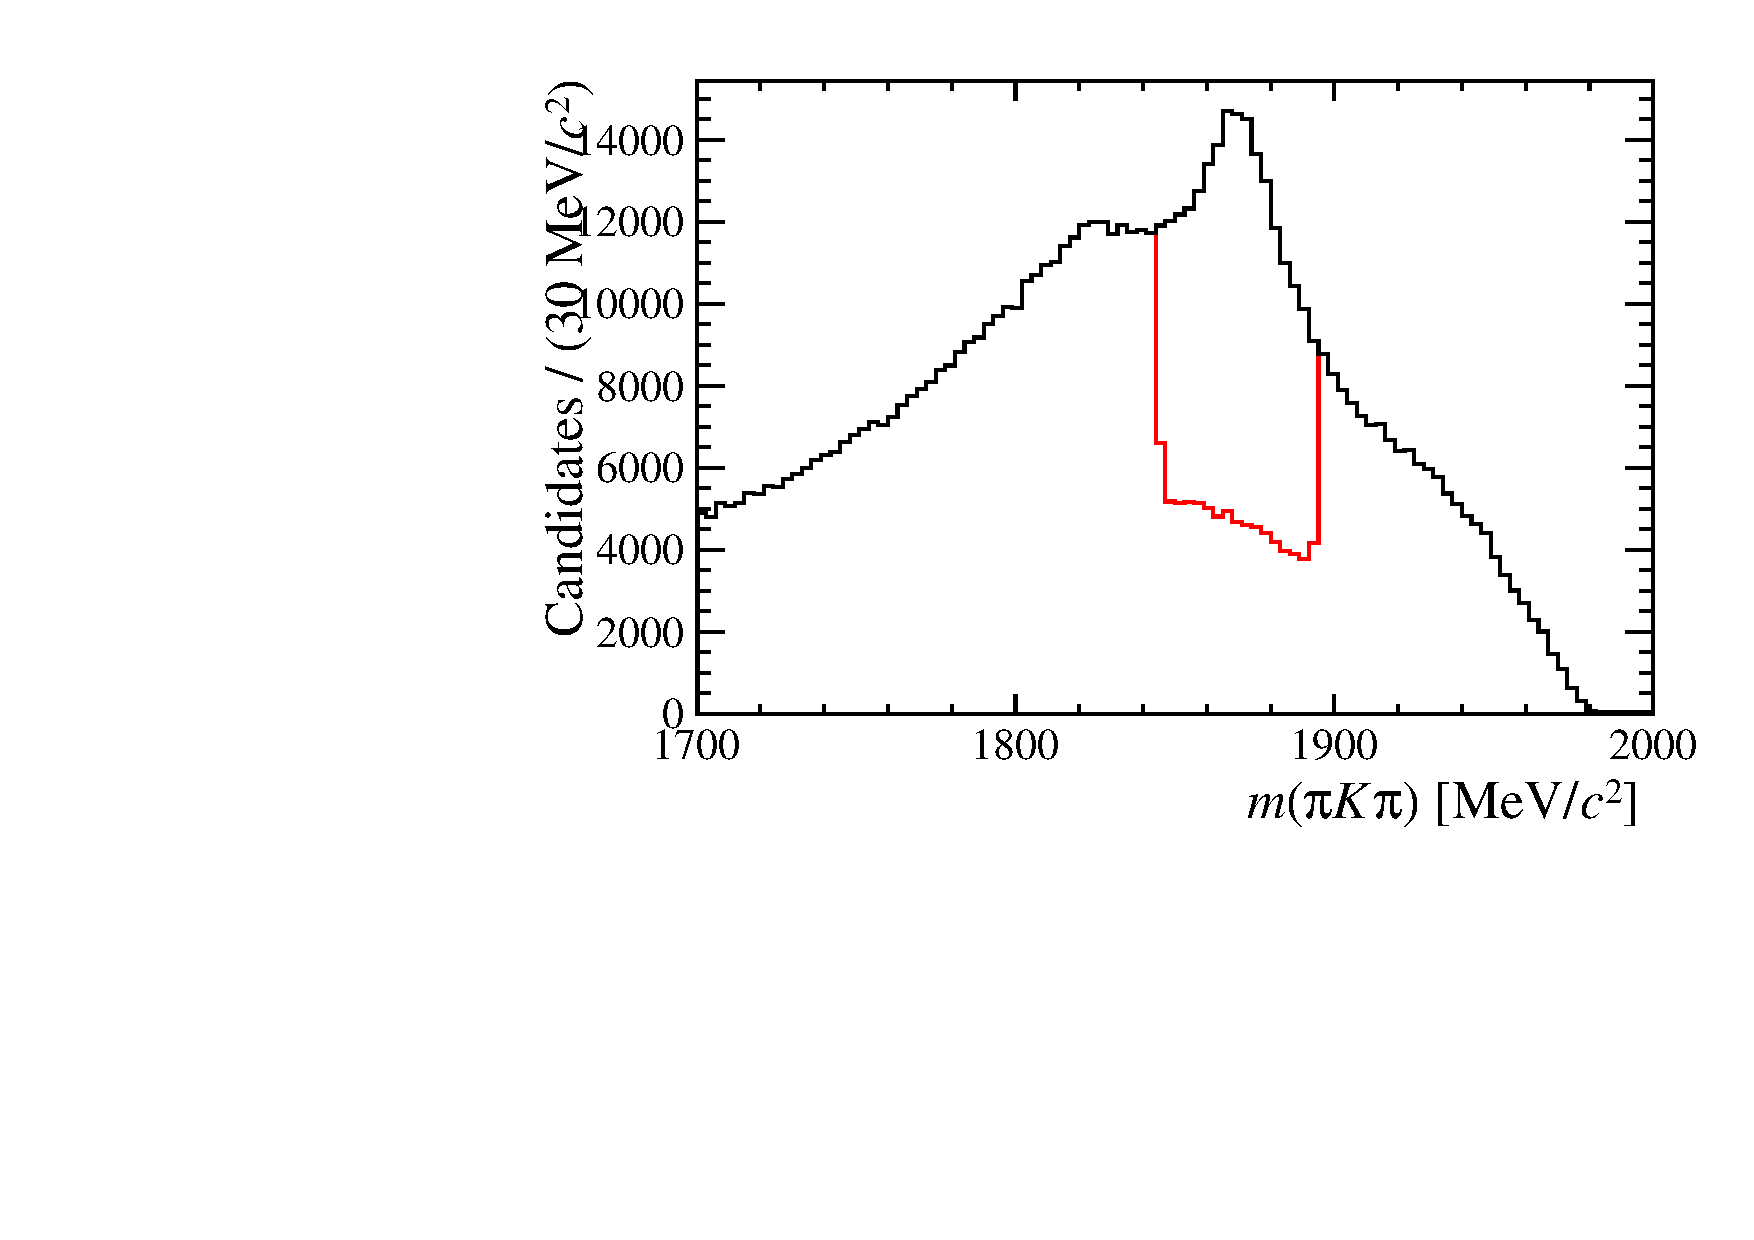
\includegraphics[width=1.0\textwidth]{figs/Selection/B2DsD0_Ds2KKPi_D_Veto_NoBDT.pdf}
        \caption{Normalisation without selection}
    \end{subfigure}%
    \begin{subfigure}[t]{0.4\textwidth}
        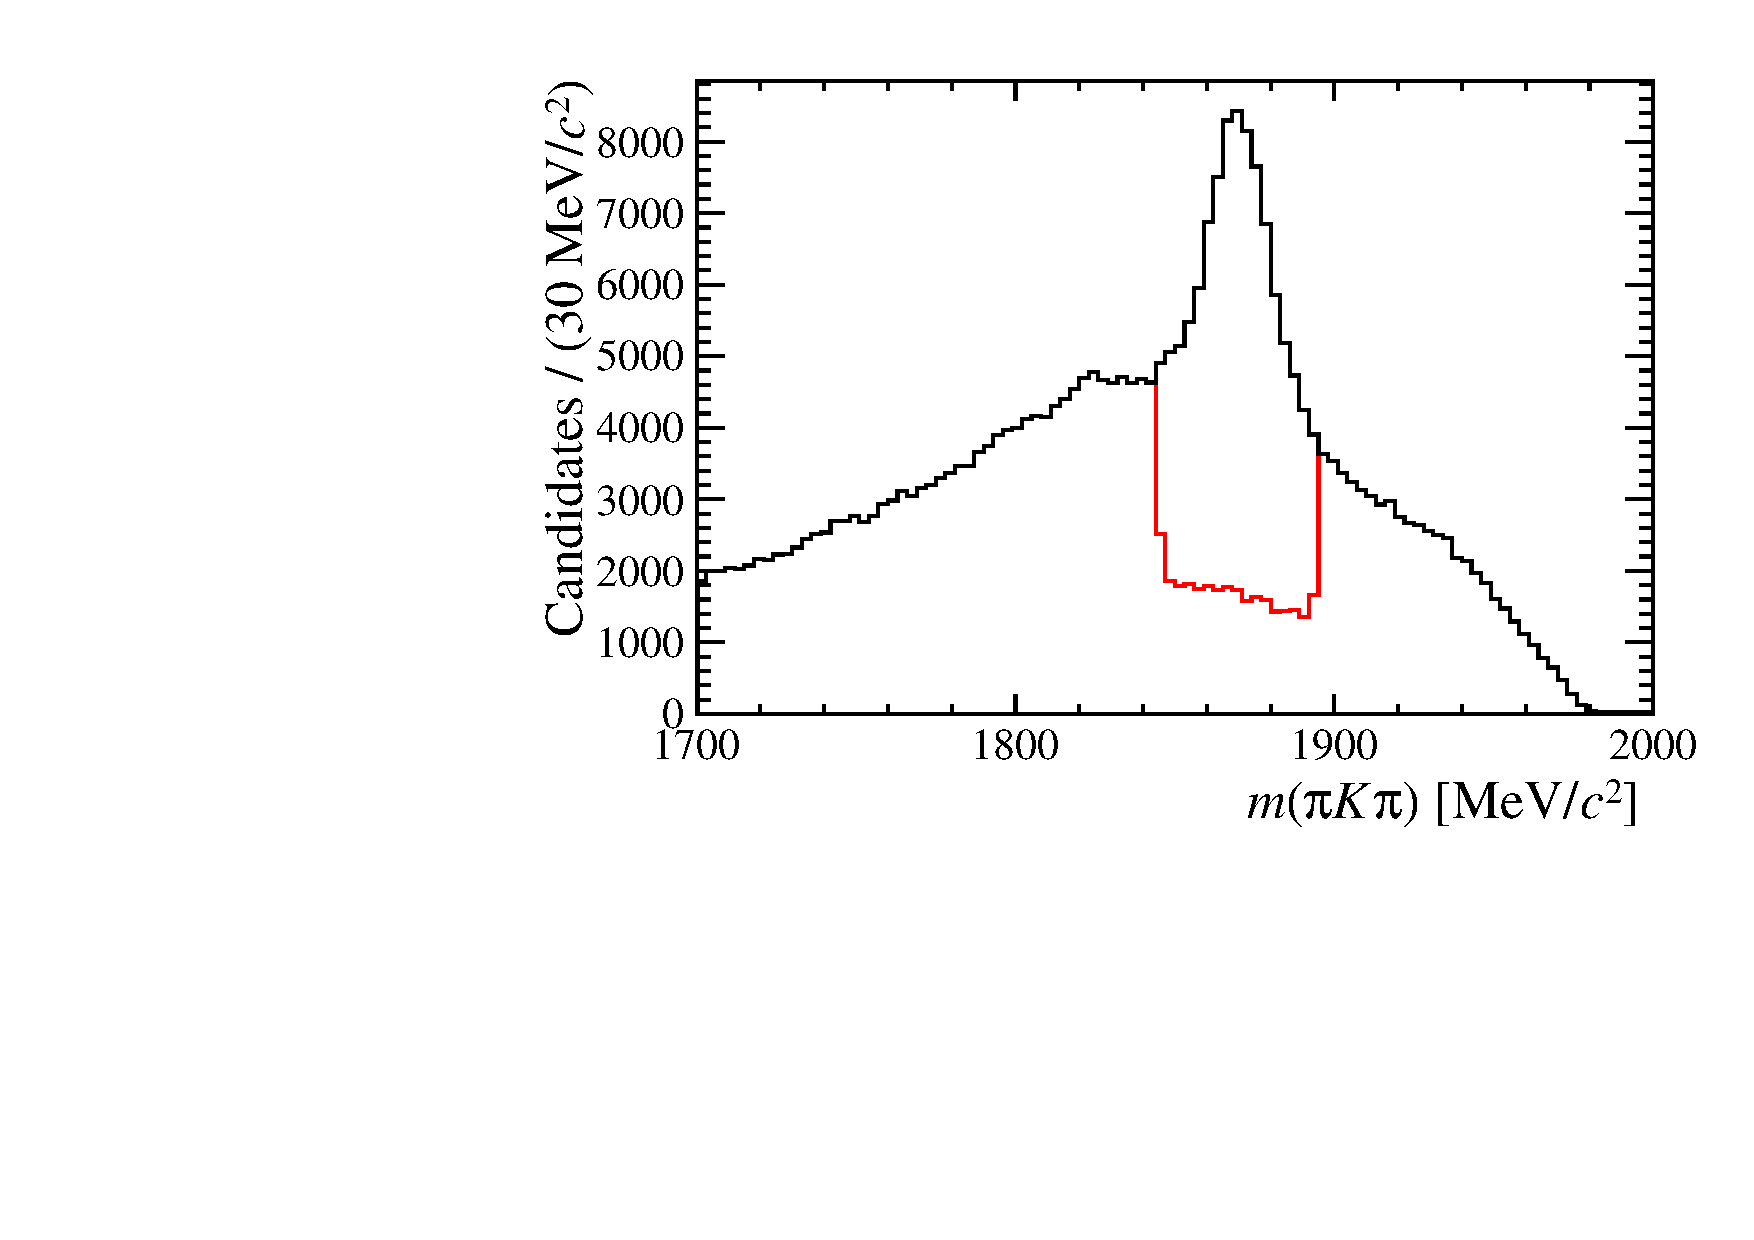
\includegraphics[width=1.0\textwidth]{figs/Selection/B2DsPhi_Ds2KKPi_D_Veto_NoBDT.pdf}
        \caption{Signal without selection}
    \end{subfigure}\\
    \begin{subfigure}[t]{0.4\textwidth}
        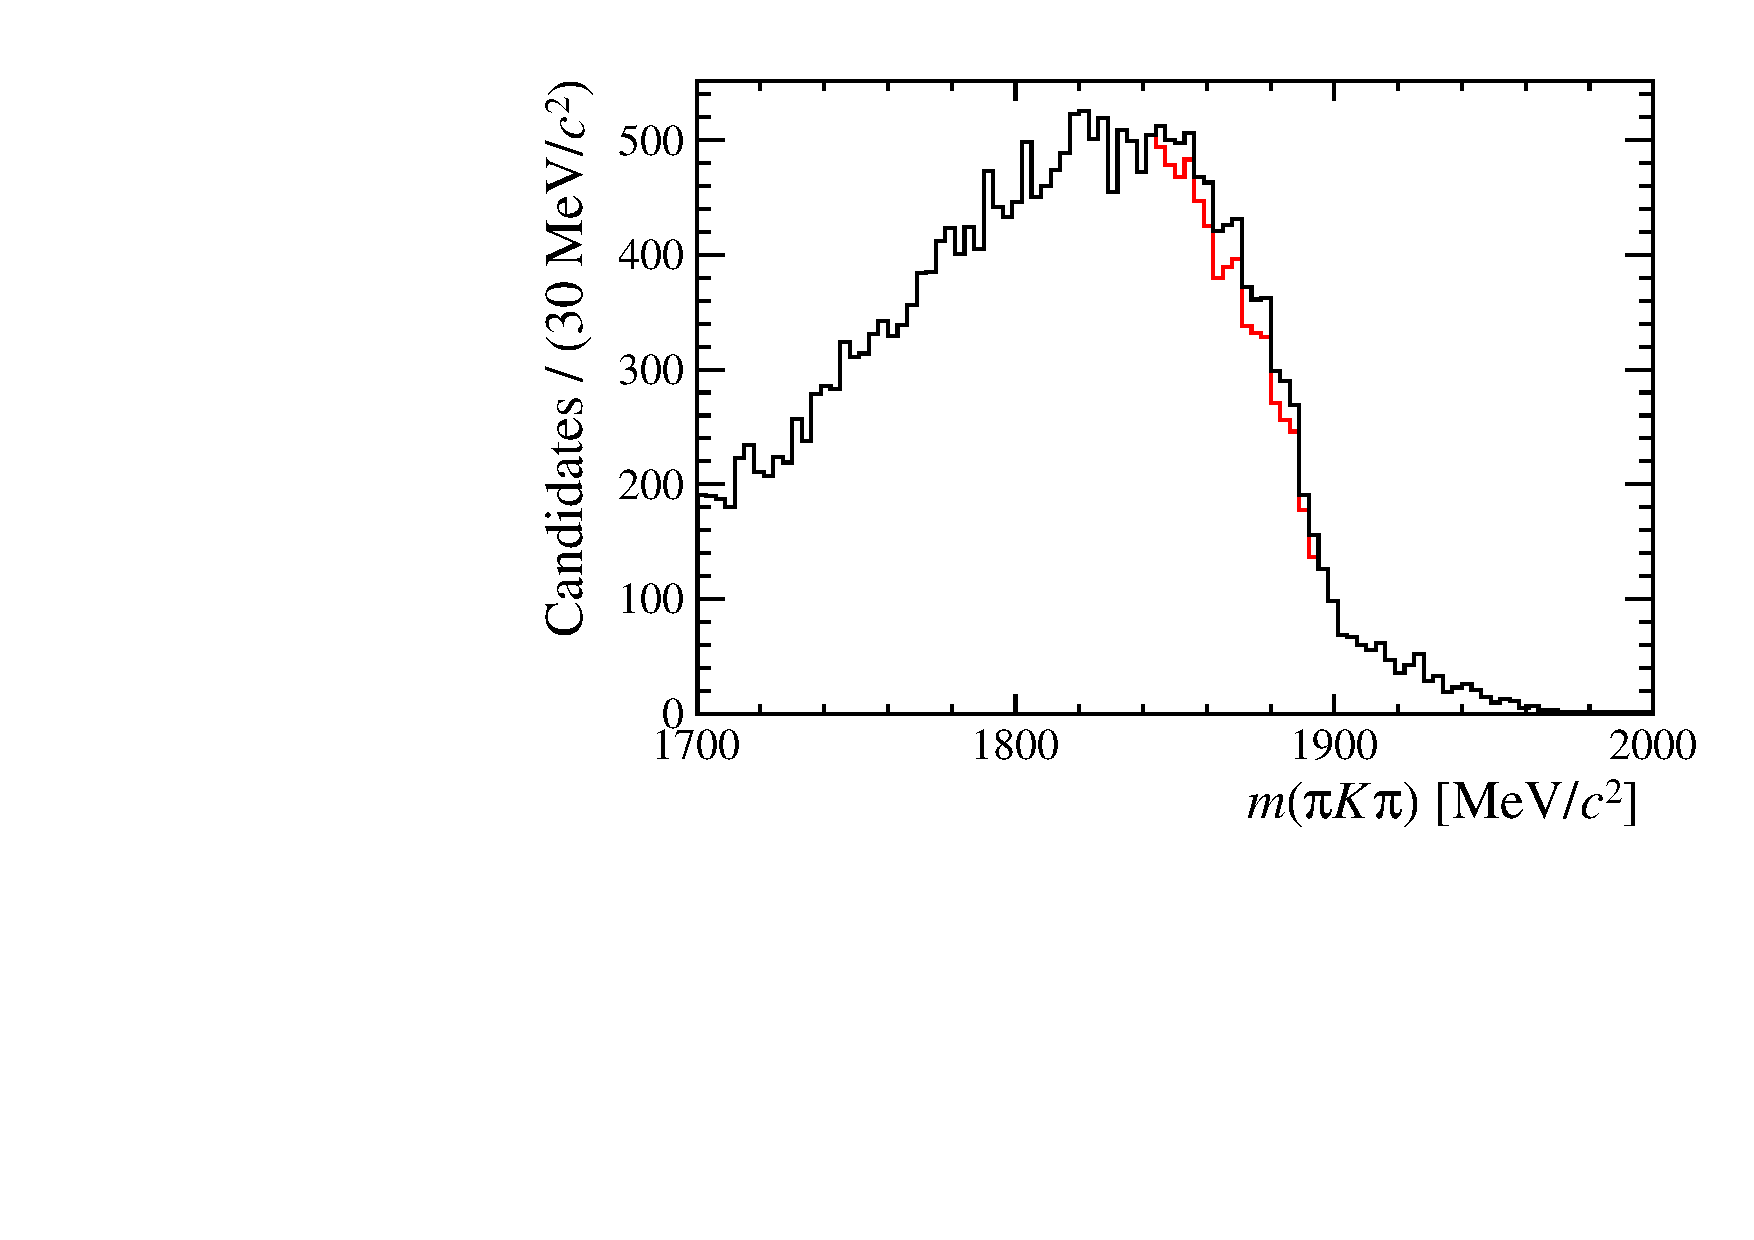
\includegraphics[width=1.0\textwidth]{figs/Selection/B2DsD0_Ds2KKPi_D_Veto_WithBDT.pdf}
        \caption{Normalisation with selection}
    \end{subfigure}%
    \begin{subfigure}[t]{0.4\textwidth}
        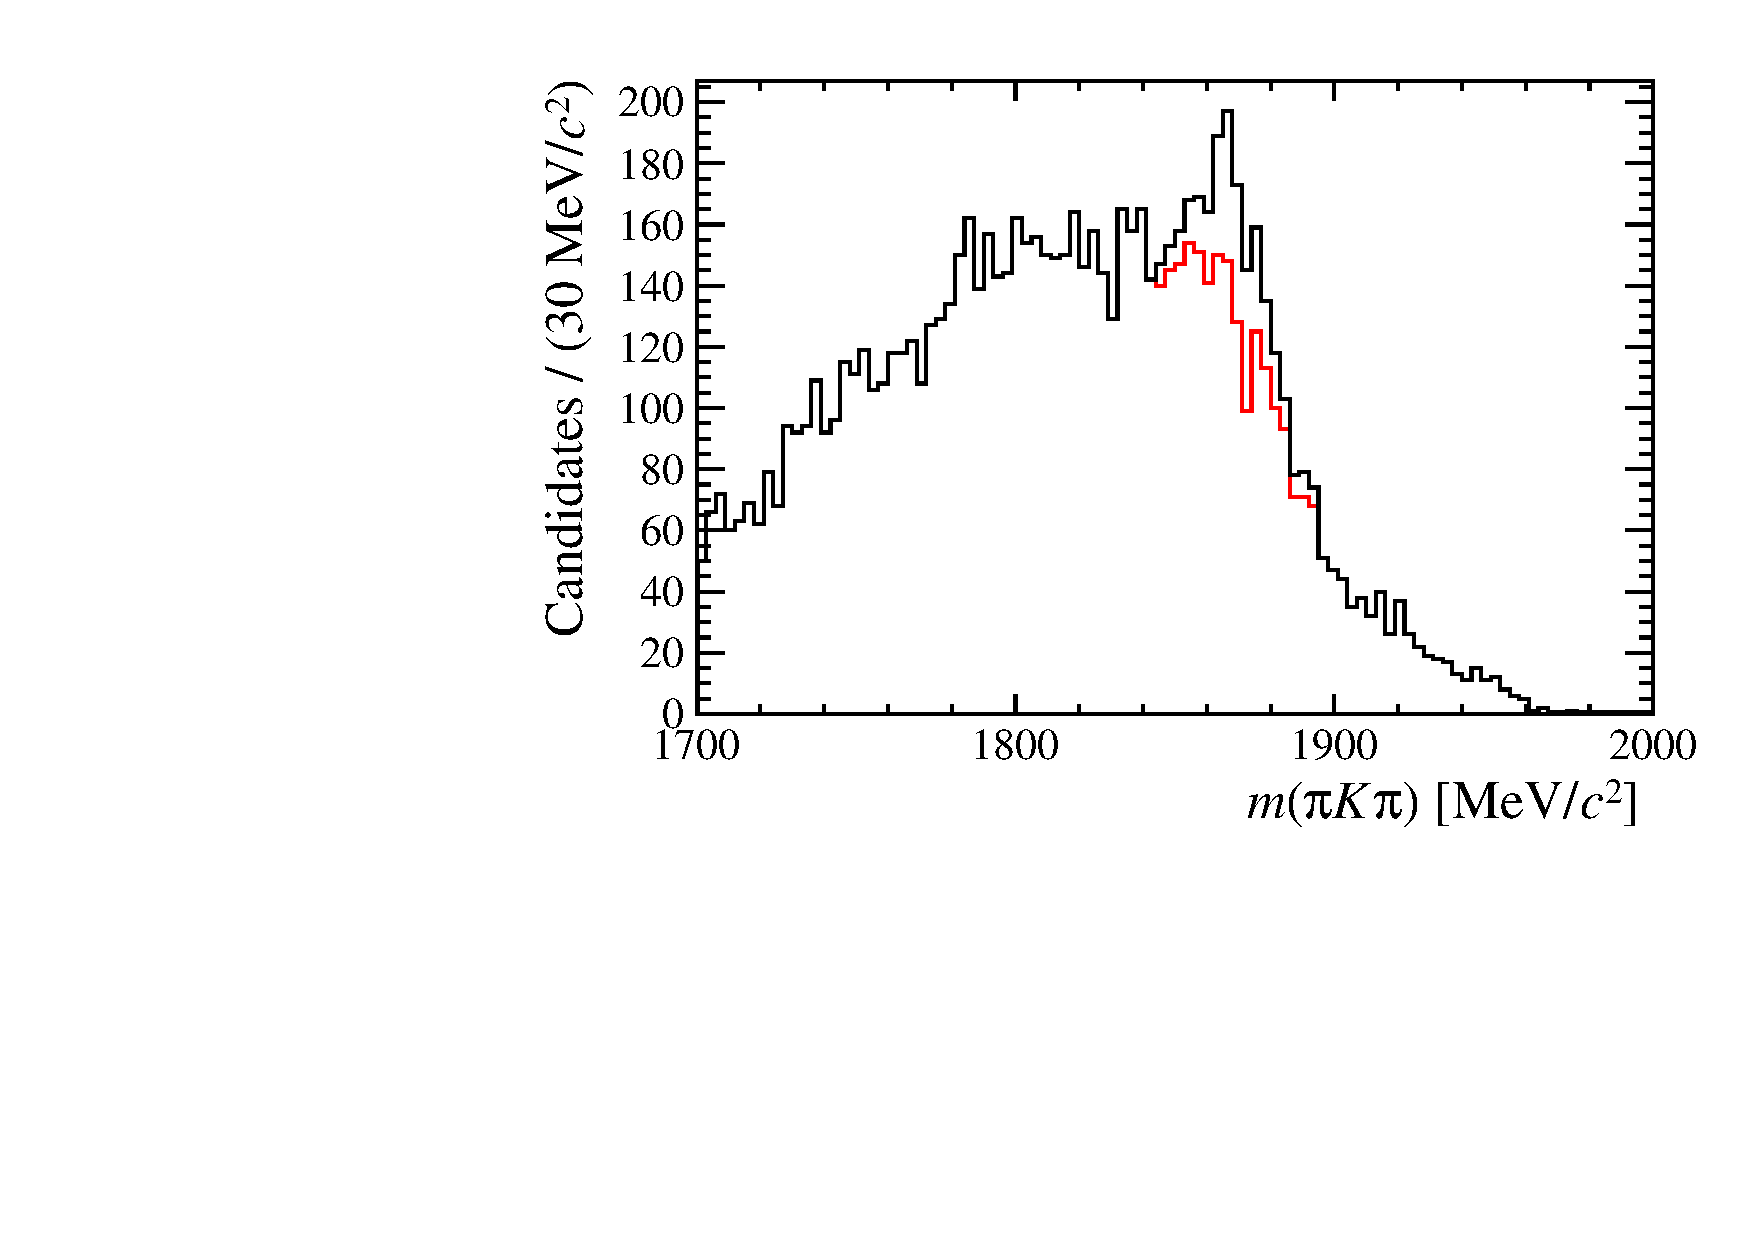
\includegraphics[width=1.0\textwidth]{figs/Selection/B2DsPhi_Ds2KKPi_D_Veto_WithBDT.pdf}
        \caption{Signal with selection}
    \end{subfigure}\\
    \caption{Invariant mass distributions of \decay{\Dsp}{\Kp\Km\pip} samples reconstructed as \decay{\Dp}{\pip\Km\pip} for the signal and normalisation samples. The samples are shown with (red) and without (black) the veto described in Sec.~\ref{sec:pidvetos}. The distributions are shown before (top) and after (bottom) the MVA requirements have been applied.}
    \label{fig:PIDVetos_Ds2KKPi_D_Veto}   
\end{figure}
%%%%%%%%%%%%%%%%%%%%%%%%%%%%%%%%%%%%%%%%%%%%%%%%%%%%%%%%%%

%%%%%%%%%%%%%%%%%%%%%%%%%%%%%%%%%%%%%%%%%%%%%%%%%%%%%%%%%%
\begin{figure}[!h]
    \centering
    \begin{subfigure}[t]{0.4\textwidth}
        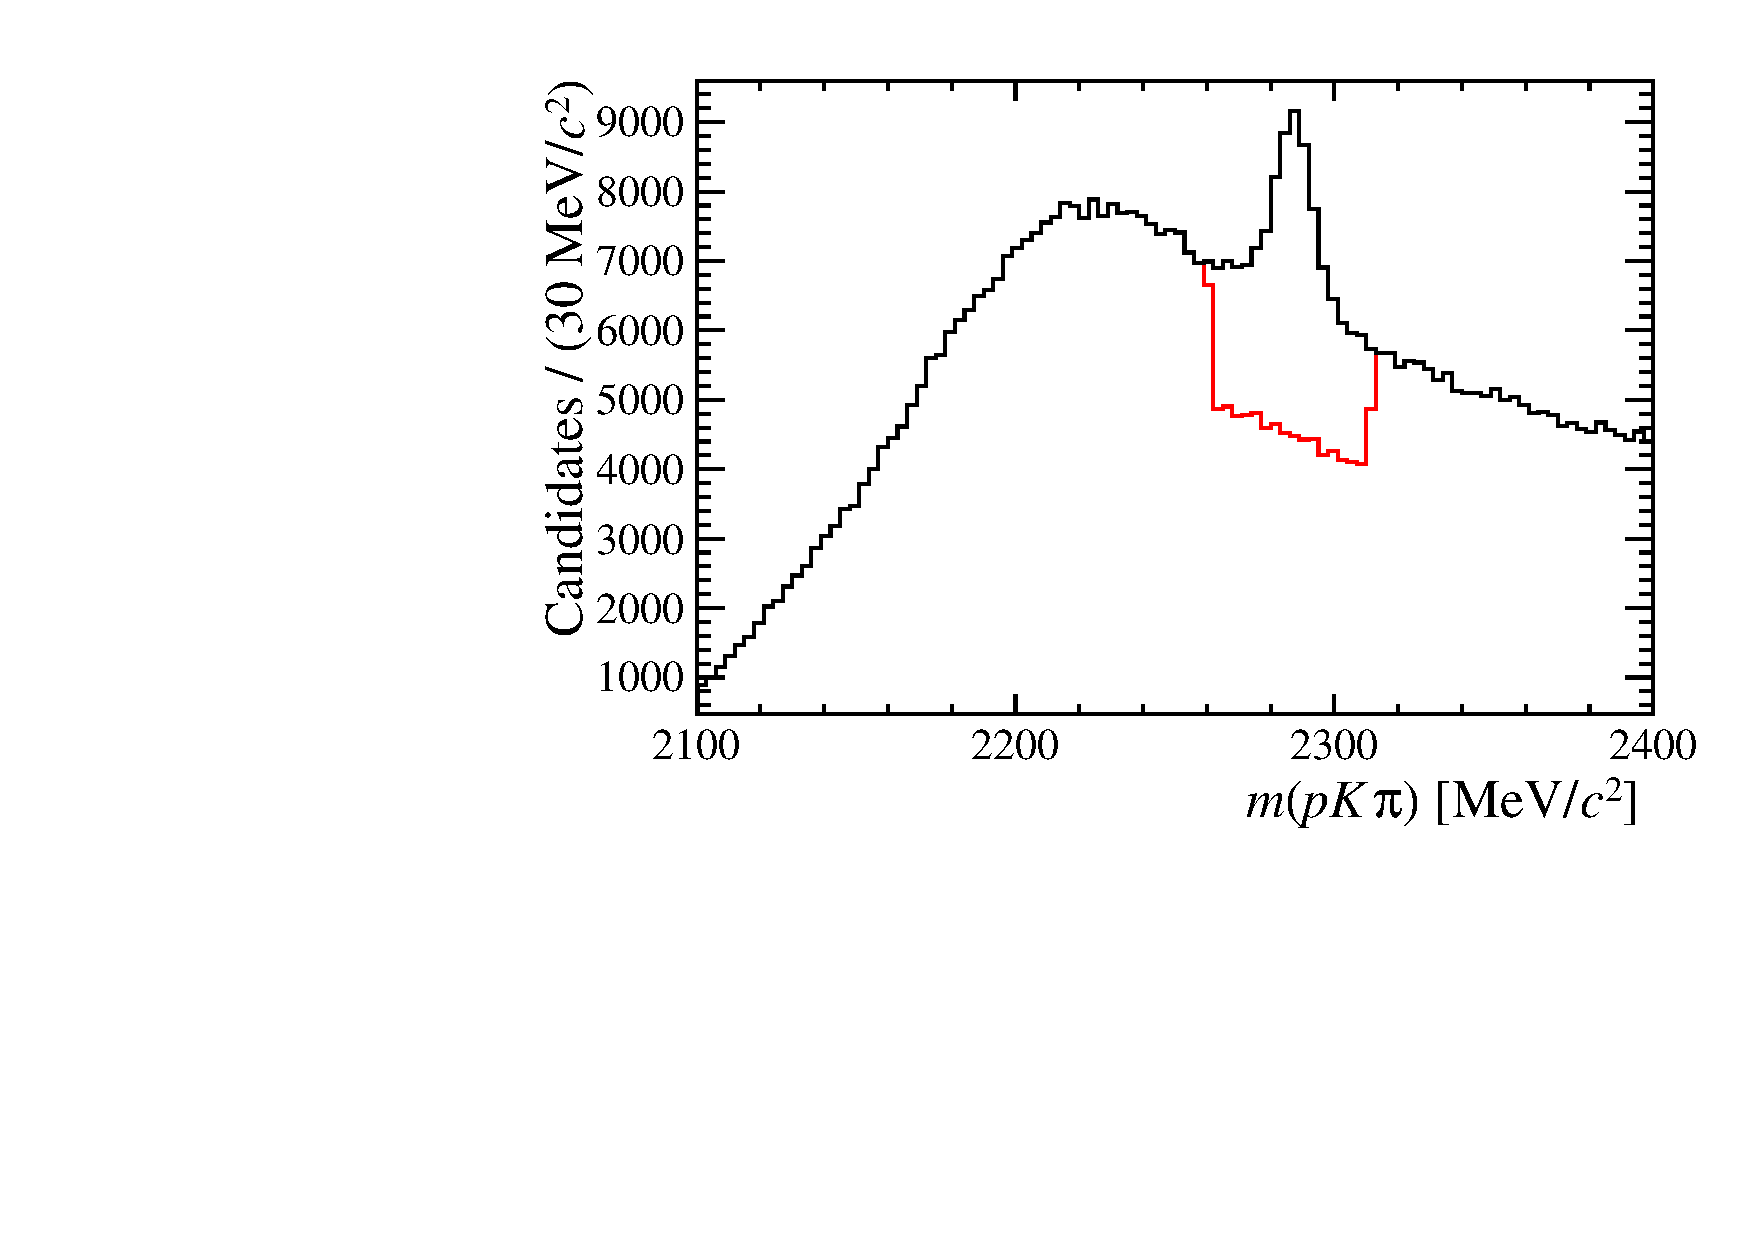
\includegraphics[width=1.0\textwidth]{figs/Selection/B2DsD0_Ds2KKPi_Lc_Veto_NoBDT.pdf}
        \caption{Normalisation without MVA cut}
    \end{subfigure}%
    \begin{subfigure}[t]{0.4\textwidth}
        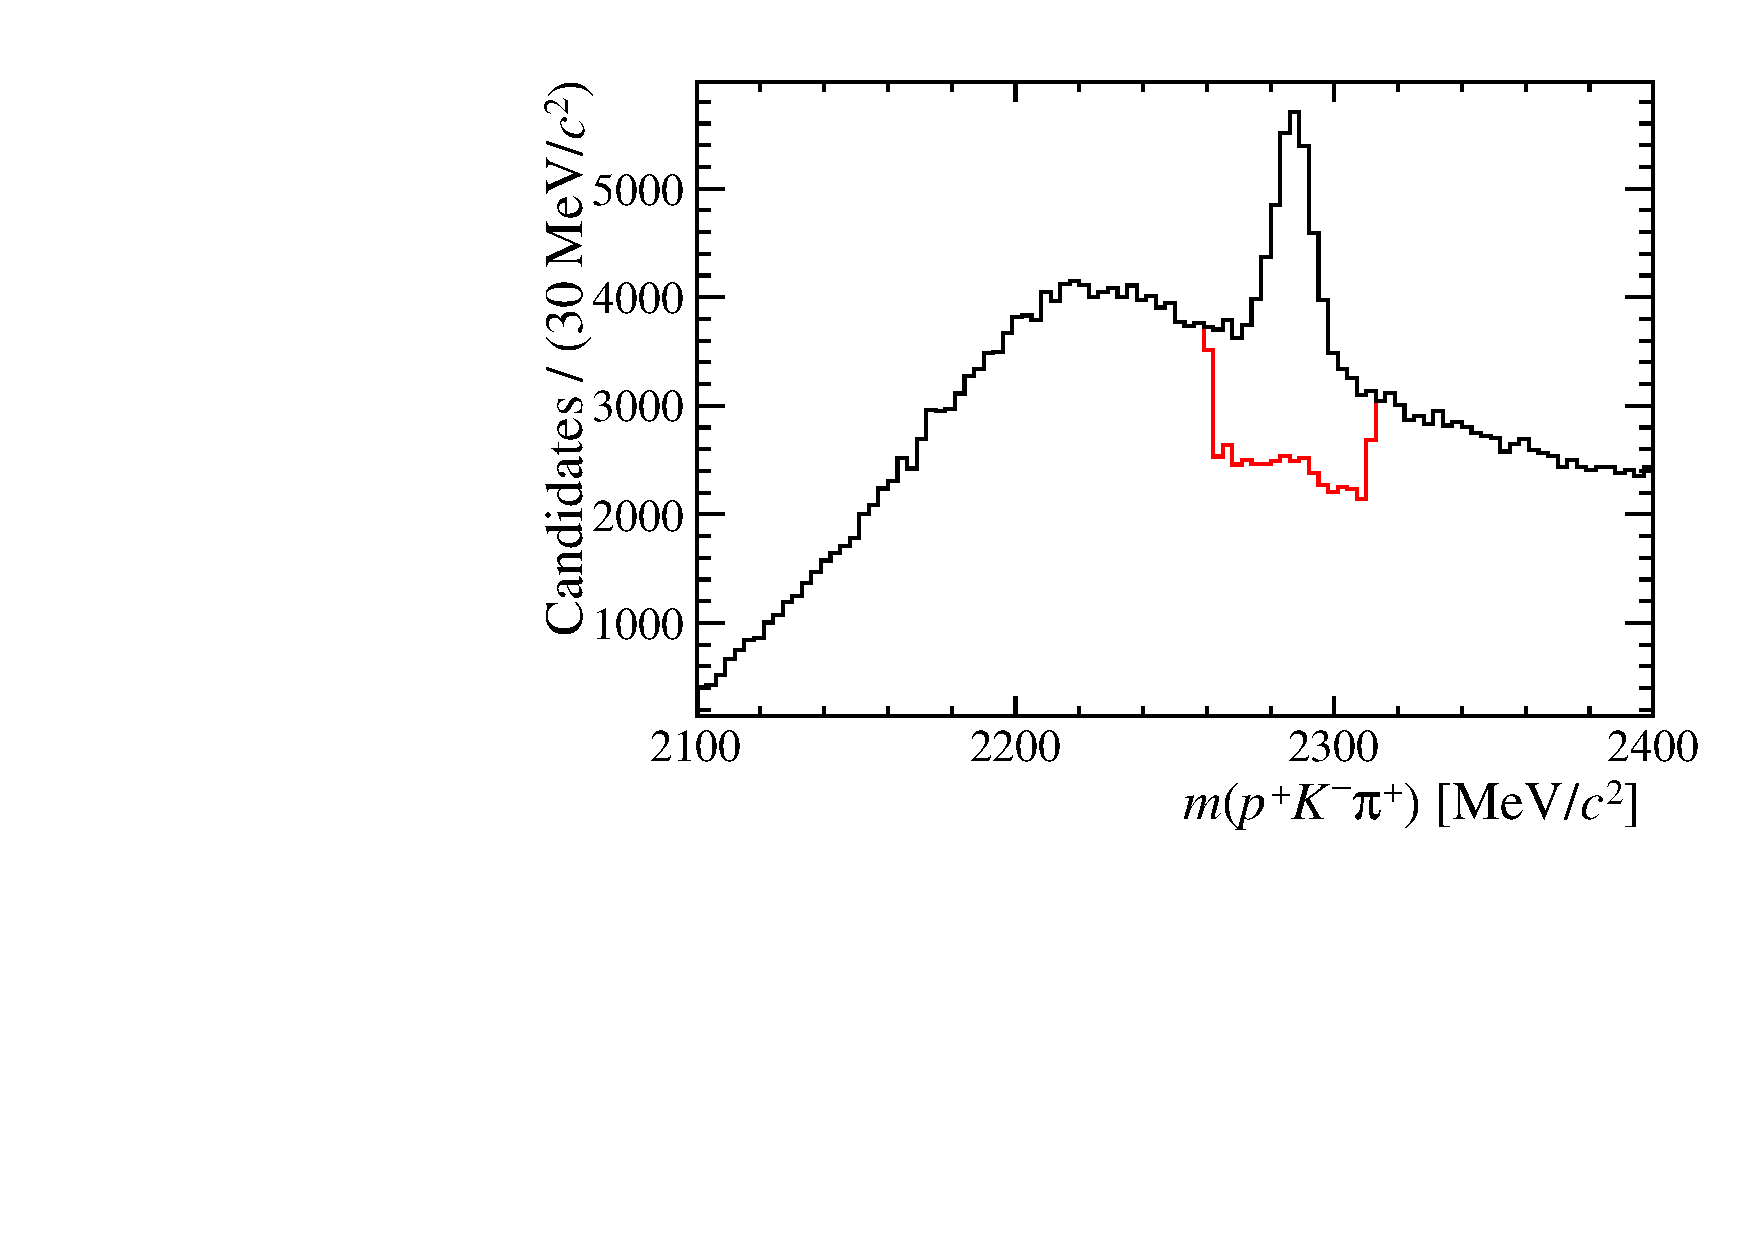
\includegraphics[width=1.0\textwidth]{figs/Selection/B2DsPhi_Ds2KKPi_Lc_Veto_NoBDT.pdf}
        \caption{Signal without MVA cut}
    \end{subfigure}\\
    \begin{subfigure}[t]{0.4\textwidth}
        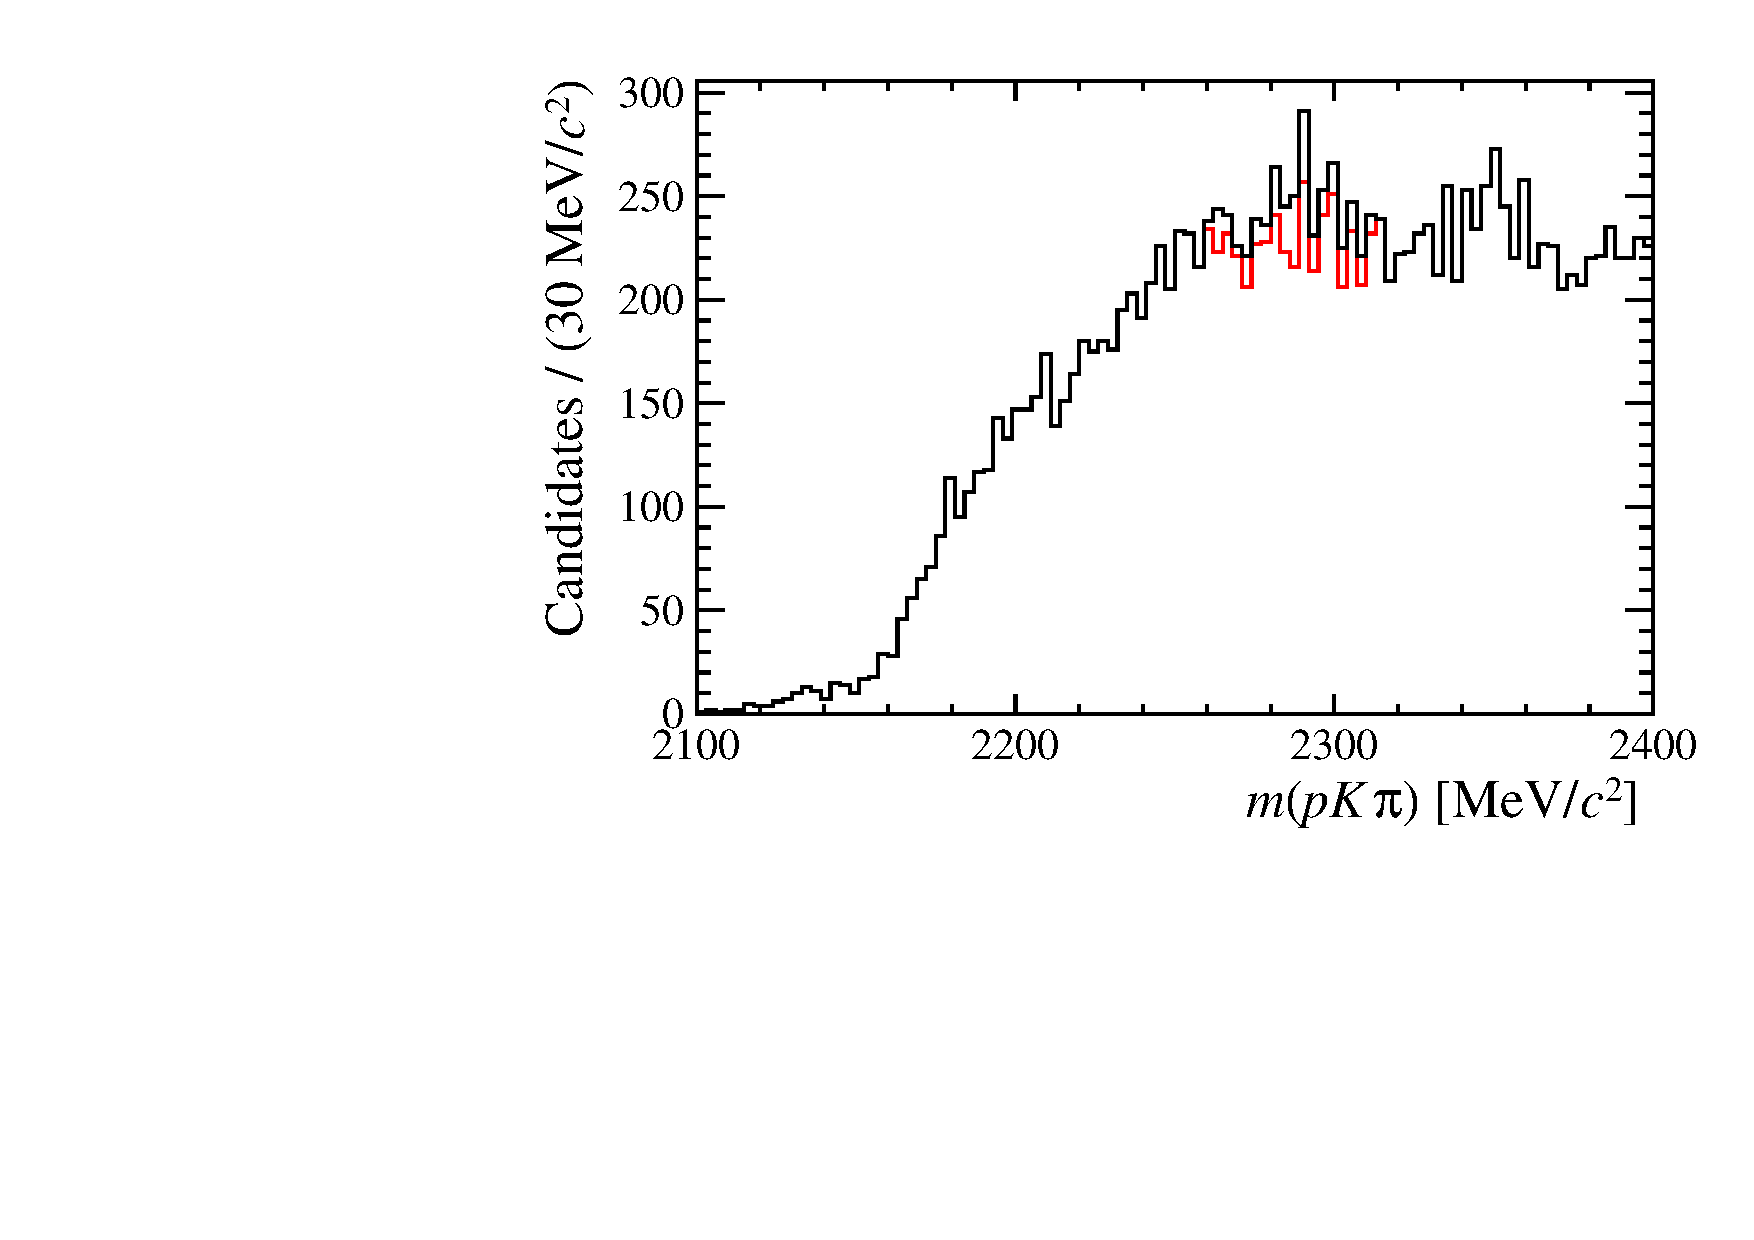
\includegraphics[width=1.0\textwidth]{figs/Selection/B2DsD0_Ds2KKPi_Lc_Veto_WithBDT.pdf}
        \caption{Normalisation with MVA cut}
    \end{subfigure}%
    \begin{subfigure}[t]{0.4\textwidth}
        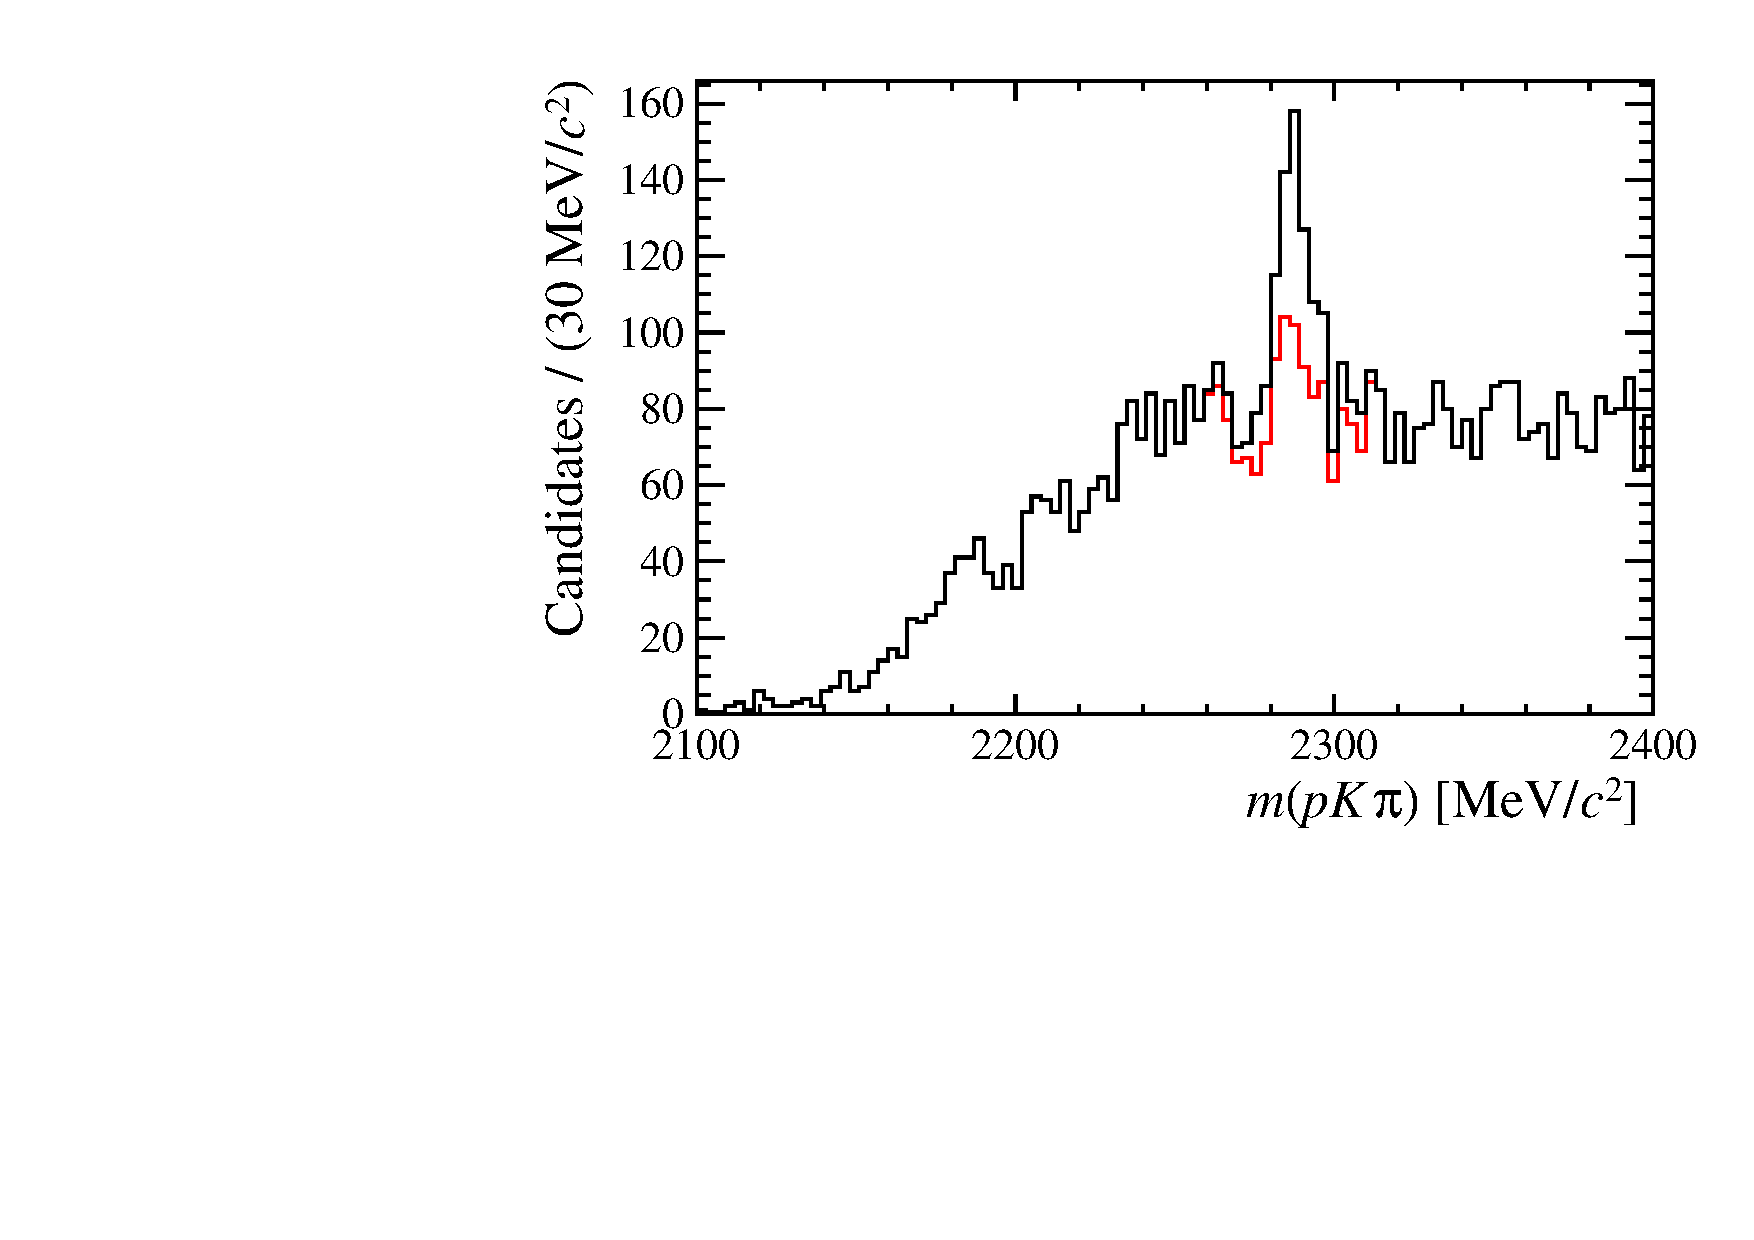
\includegraphics[width=1.0\textwidth]{figs/Selection/B2DsPhi_Ds2KKPi_Lc_Veto_WithBDT.pdf}
        \caption{Signal with MVA cut}
    \end{subfigure}\\
    \caption{Invariant mass distributions of \decay{\Dsp}{\Kp\Km\pip} samples reconstructed as \decay{\Lc}{\Pp\Km\pip} for the signal and normalisation samples. The samples are shown with (red) and without (black) the veto described in Sec.~\ref{sec:pidvetos}. The distributions are shown before (top) and after (bottom) the MVA requirements have been applied.}
    \label{fig:PIDVetos_Ds2KKPi_Lc_Veto}   
\end{figure}
%%%%%%%%%%%%%%%%%%%%%%%%%%%%%%%%%%%%%%%%%%%%%%%%%%%%%%%%%%

\subsection{Invariant mass vetoes}
\label{sec:kinematicvetos}

Sharp peaking structures are observed in subsets of the final state particles. These are removed with simple invariant mass cuts to remove combinatorial or partially reconstructed backgrounds that result from these incorrectly reconstructed decays. 
For simplicity the final state particles for each mode are labelled with a number between 1--5 as described in Table~\ref{table:vetolabels}.

\begin{table*}[!ht]
\centering
\begin{tabular}{ l c c c c c c }
\hline
Decay Mode & 1  & 2 & 3 & 4 & 5 \\
\hline
\decay{\Bp}{(\decay{\Dsp}{\Kp\Km\pip})\phiz}       & \Kp    & \Km    & \pip  & \Kp  & \Km \\
\decay{\Bp}{(\decay{\Dsp}{\pip\pim\pip})\phiz}     & \pip   & \pim   & \pip  & \Kp  & \Km \\
\decay{\Bp}{(\decay{\Dsp}{\Kp\pim\pip})\phiz}      & \Kp    & \pim   & \pip  & \Kp  & \Km \\
\hline
\decay{\Bp}{(\decay{\Dsp}{\Kp\Km\pip})\Kp\Km}      & \Kp    & \Km    & \pip  & \Kp  & \Km \\
\hline
\end{tabular}
\caption{Particle labels used when studying invariant mass vetoes for \decay{\Bp}{\Dsp\phiz} and \decay{\Bp}{\Dsp\Kp\Km} candidates.}
\label{table:vetolabels}

\end{table*}

All combinations of the final state particles that create a neutral or singly-charged candidate are investigated.
Significant structures are observed for all three \Dsp decay modes in some combination. 

The following vetos are applied to remove these incorrectly reconstructed decays.
\begin{itemize}
\item For the mode \decay{\Bp}{(\decay{\Dsp}{\Kp\Km\pip})\phiz}
\begin{itemize}
\item $|m(\text{1245})- m(\Bs)| > 50\mevcc$
\item $|m(\text{345})- m(\Dsp)| > 25\mevcc$ and $|m(\text{345})- m(\Dp)| > 25\mevcc$
\end{itemize}

\item For the mode \decay{\Bp}{(\decay{\Dsp}{\pip\pim\pip})\phiz}
\begin{itemize}
\item $|m(\text{145})- m(\Dsp)| > 25\mevcc$ and $|m(\text{145})- m(\Dp)| > 25\mevcc$
\item $|m(\text{245})- m(\Dsp)| > 25\mevcc$ and $|m(\text{245})- m(\Dp)| > 25\mevcc$
\item $|m(\text{345})- m(\Dsp)| > 25\mevcc$ and $|m(\text{345})- m(\Dp)| > 25\mevcc$
\end{itemize}
\item For the mode \decay{\Bp}{(\decay{\Dsp}{\Kp\pim\pip})\phiz}
\begin{itemize}
\item $|m(\text{245})- m(\Dsp)| > 25\mevcc$ and $|m(\text{245})- m(\Dp)| > 25\mevcc$
\item $|m(\text{345})- m(\Dsp)| > 25\mevcc$ and $|m(\text{345})- m(\Dp)| > 25\mevcc$
\end{itemize}
\end{itemize}

%%%%%%%%%%%%%%%%%%%%%%%%%%%%%%%%%%%%%%%%%%%%%%%%%%%%%%%%%%
\begin{figure}[!h]
   \centering
   \begin{subfigure}[t]{1.0\textwidth}
      \centering
      \begin{subfigure}[t]{0.32\textwidth}
         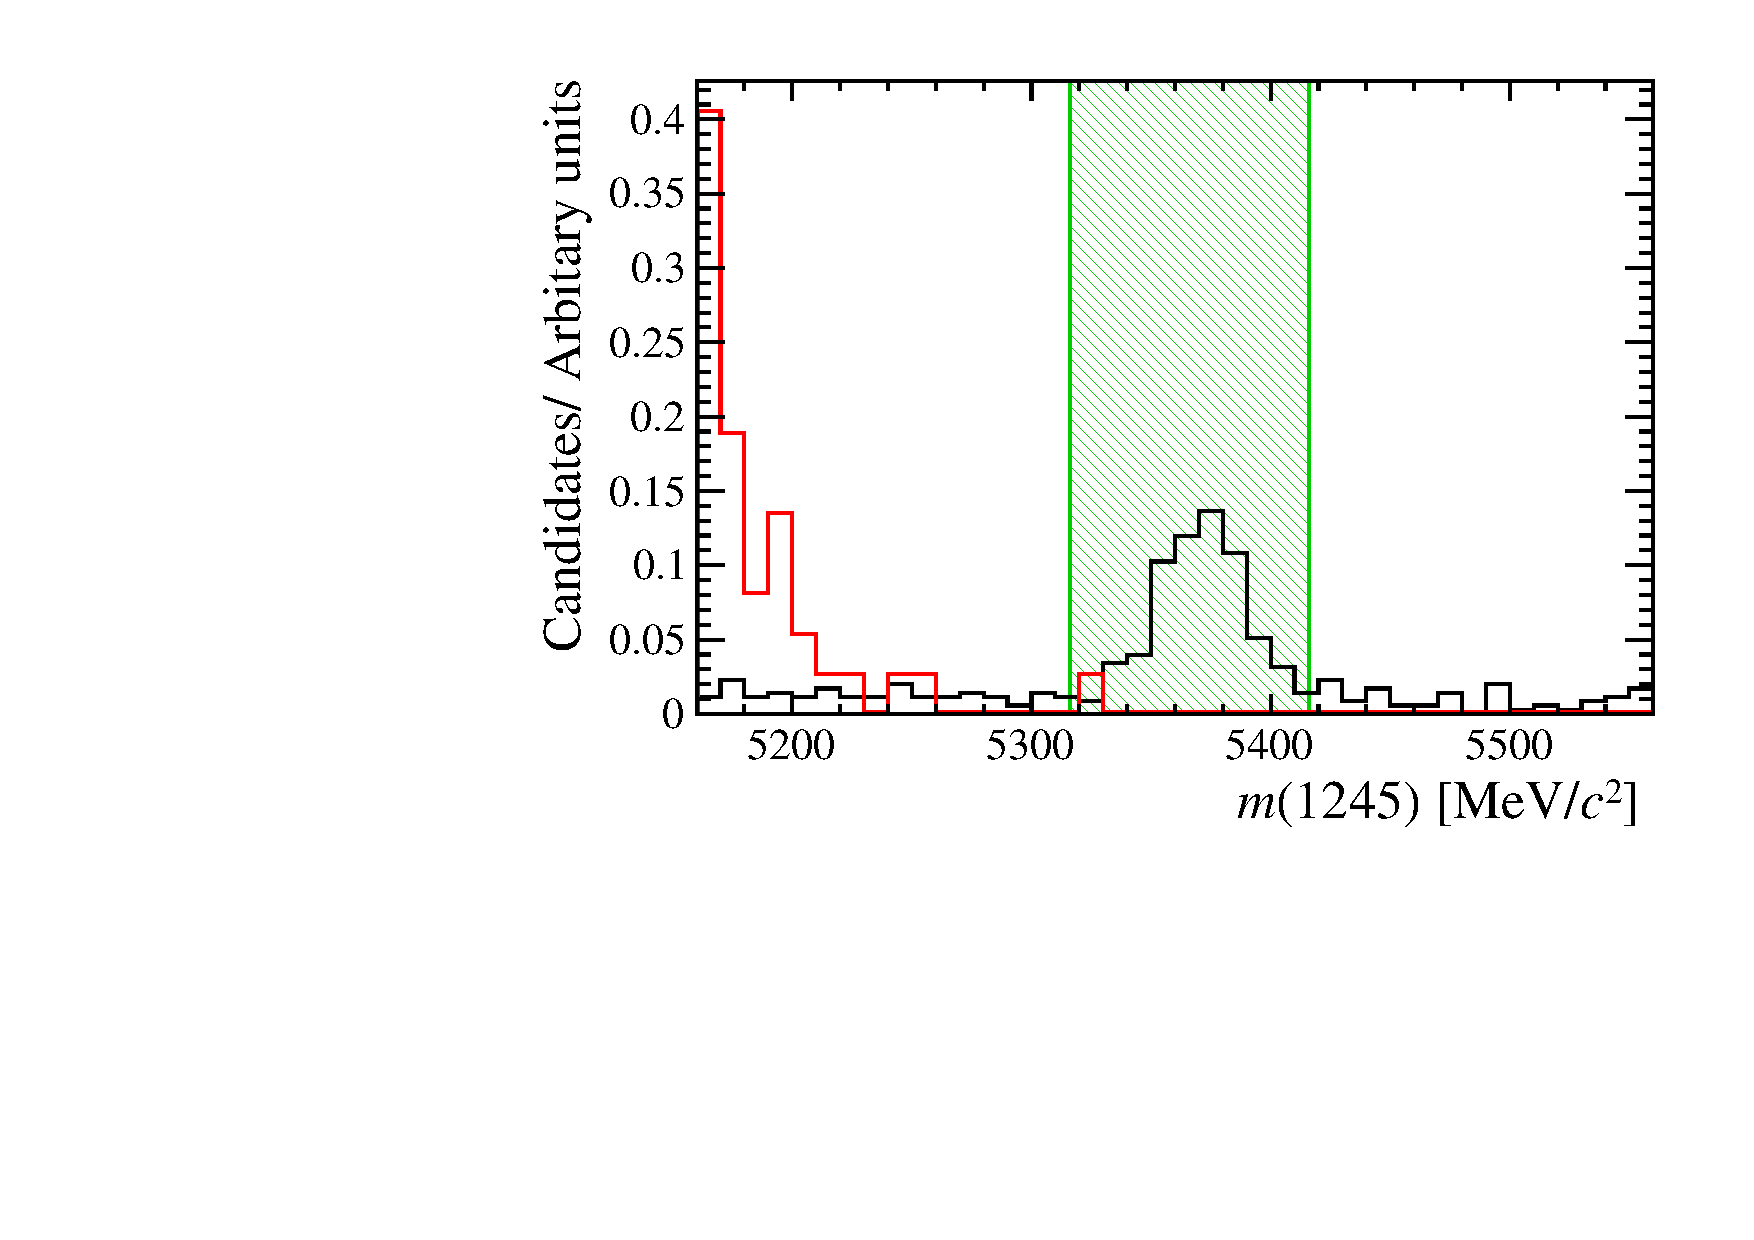
\includegraphics[width=1.0\textwidth]{figs/Selection/Veto_Comparison_B2DsPhi_Ds2KKPi_m1245.pdf}
      \end{subfigure}
      \begin{subfigure}[t]{0.32\textwidth}
         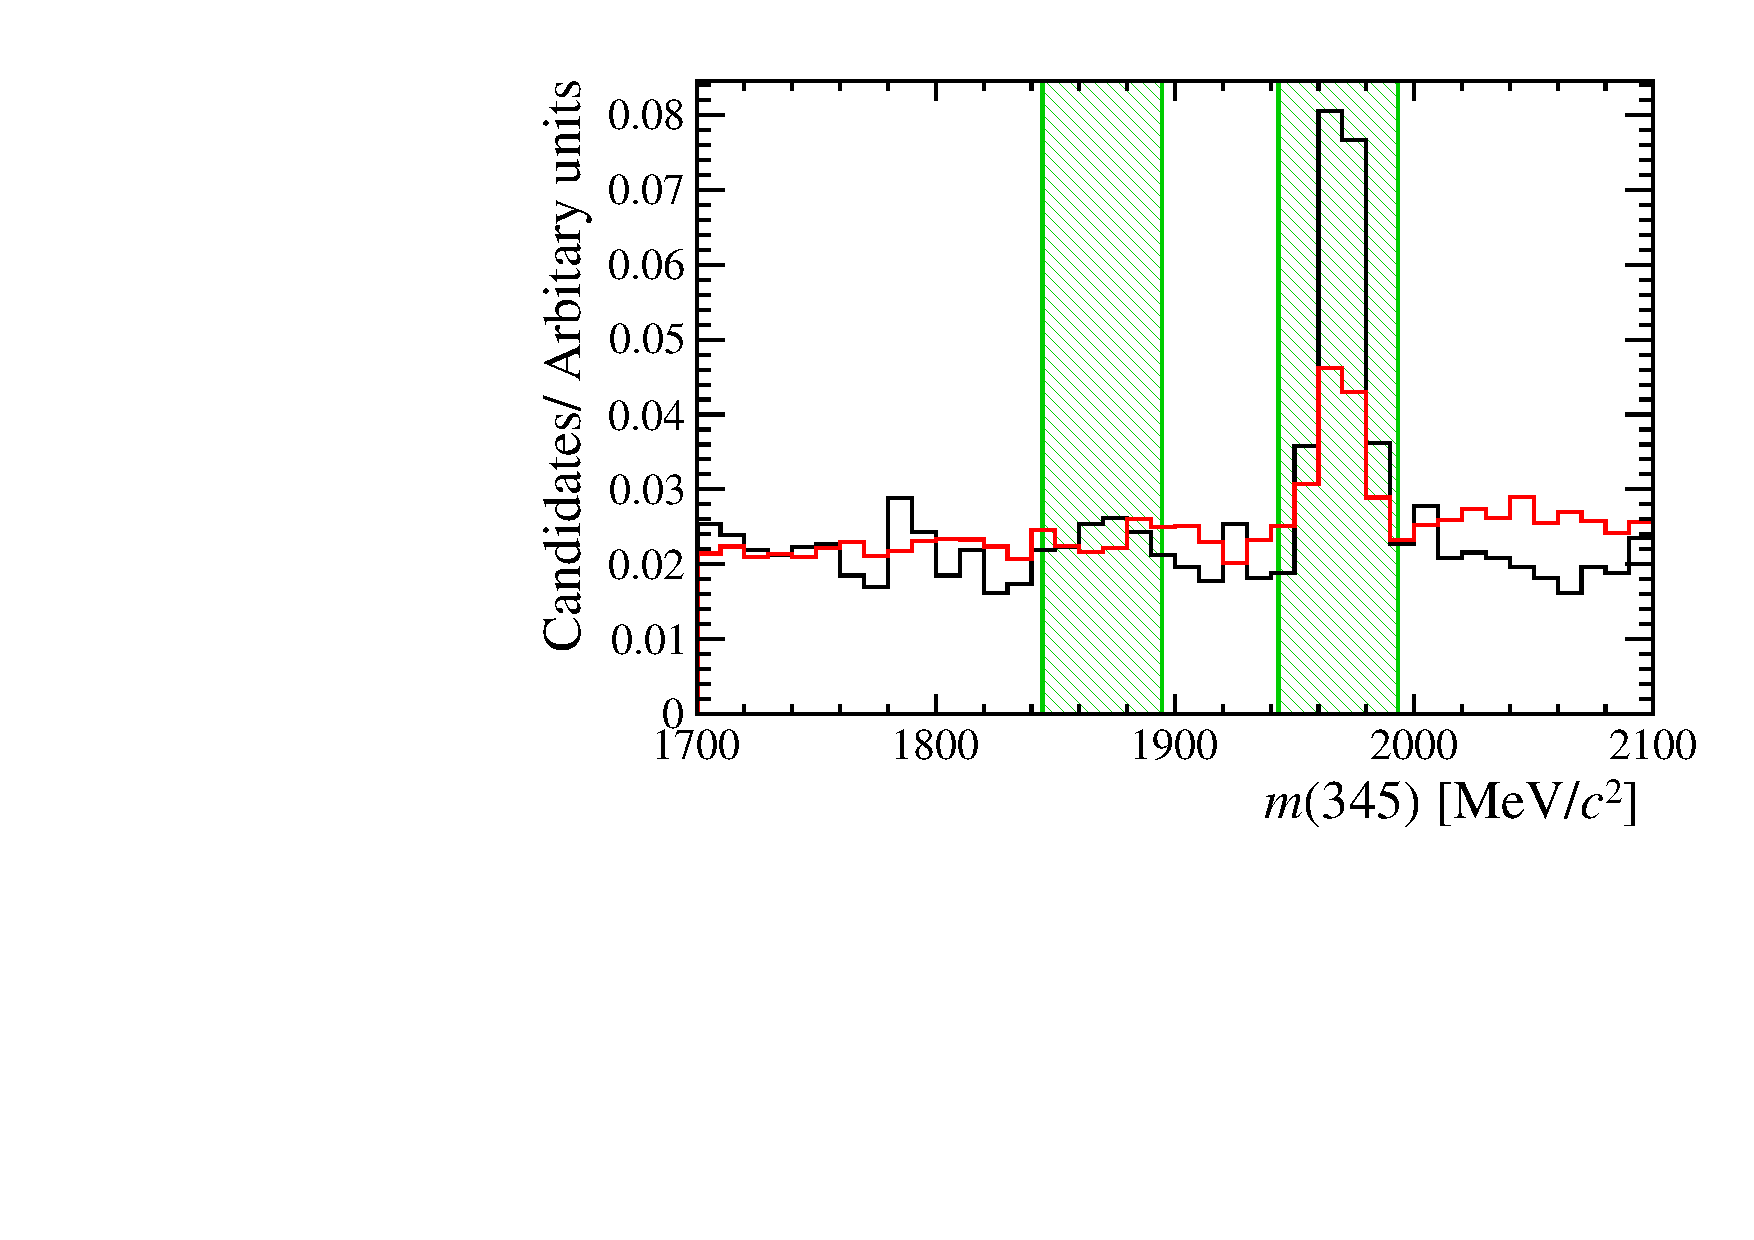
\includegraphics[width=1.0\textwidth]{figs/Selection/Veto_Comparison_B2DsPhi_Ds2KKPi_m345.pdf}
      \end{subfigure}
      \caption{\decay{\Bp}{(\decay{\Dsp}{\Kp\Km\pip})\phiz}}
   \end{subfigure}
   \begin{subfigure}[t]{1.0\textwidth}
      \centering
      \begin{subfigure}[t]{0.32\textwidth}
         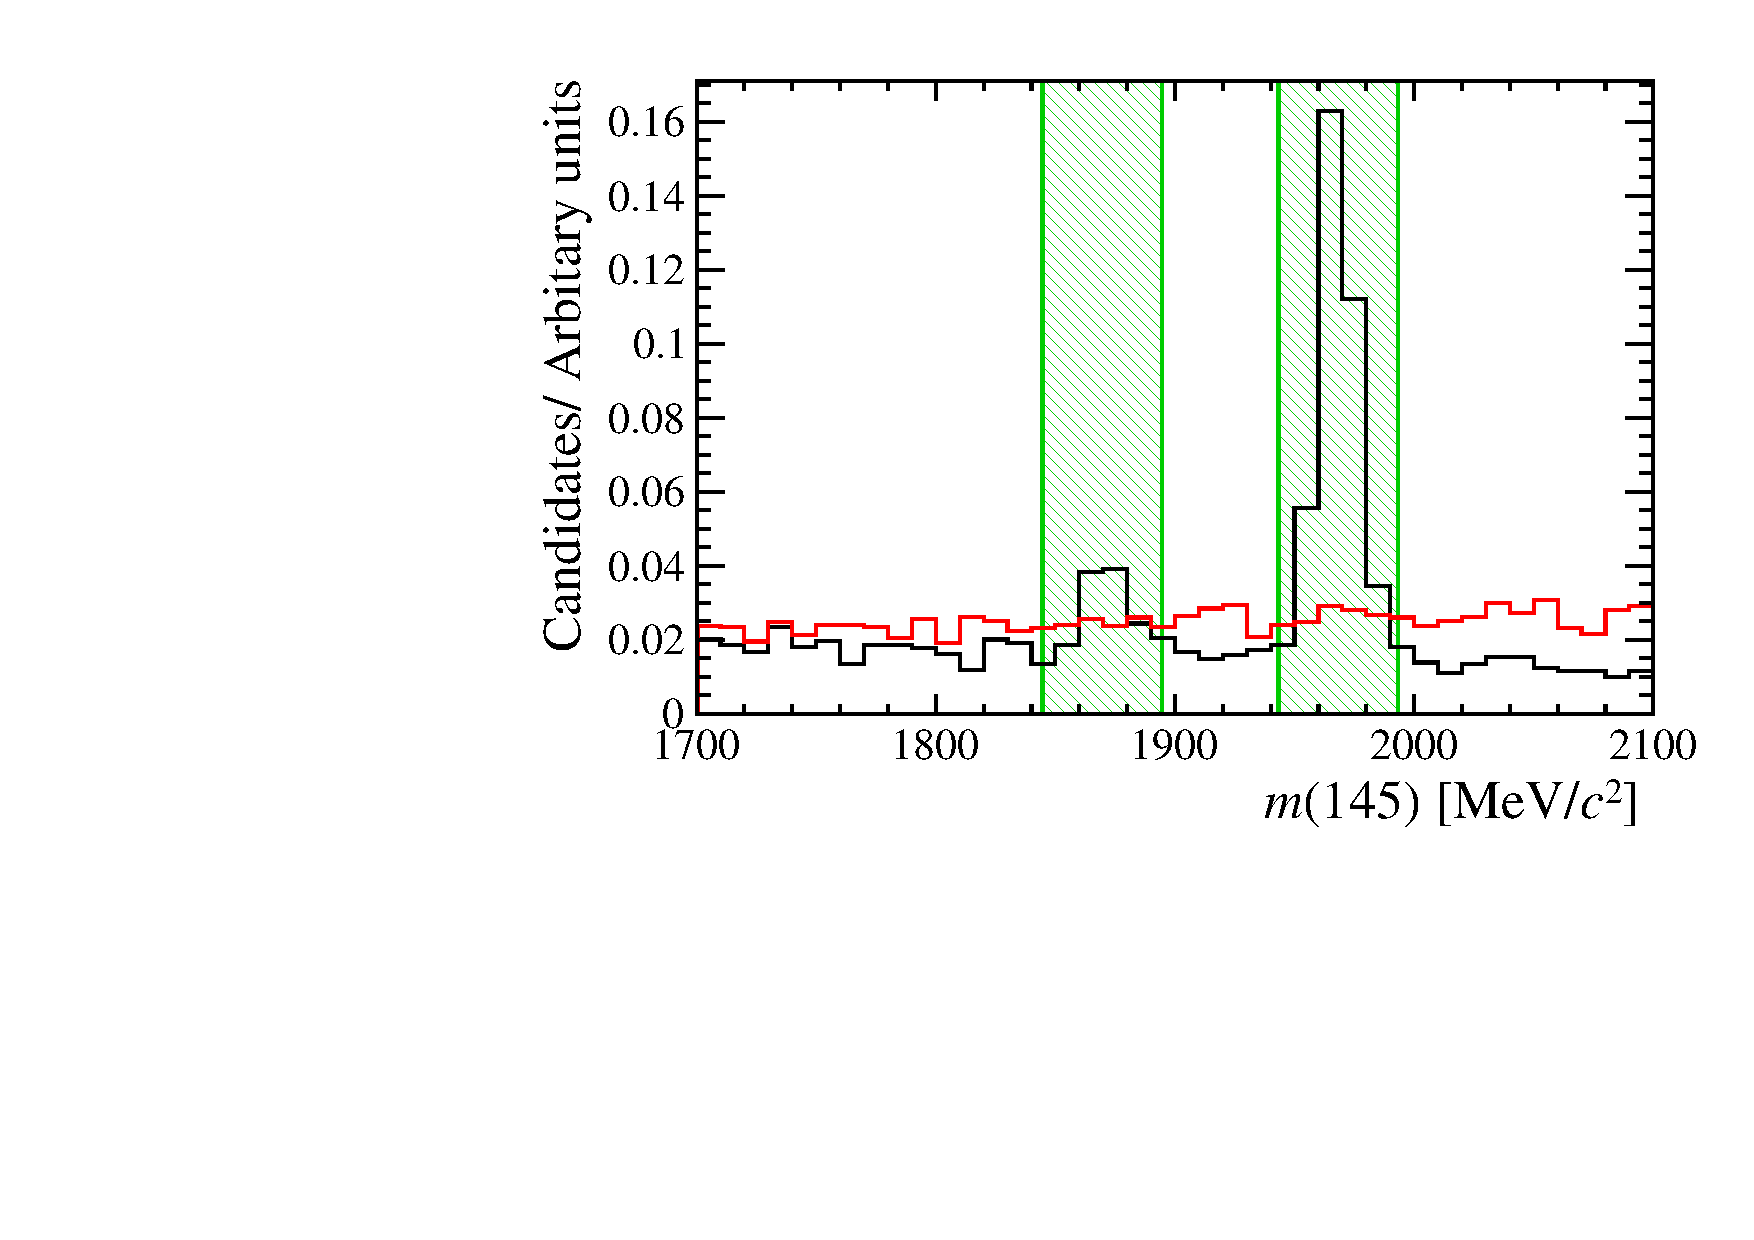
\includegraphics[width=1.0\textwidth]{figs/Selection/Veto_Comparison_B2DsPhi_Ds2PiPiPi_m145.pdf}
      \end{subfigure}
      \begin{subfigure}[t]{0.32\textwidth}
         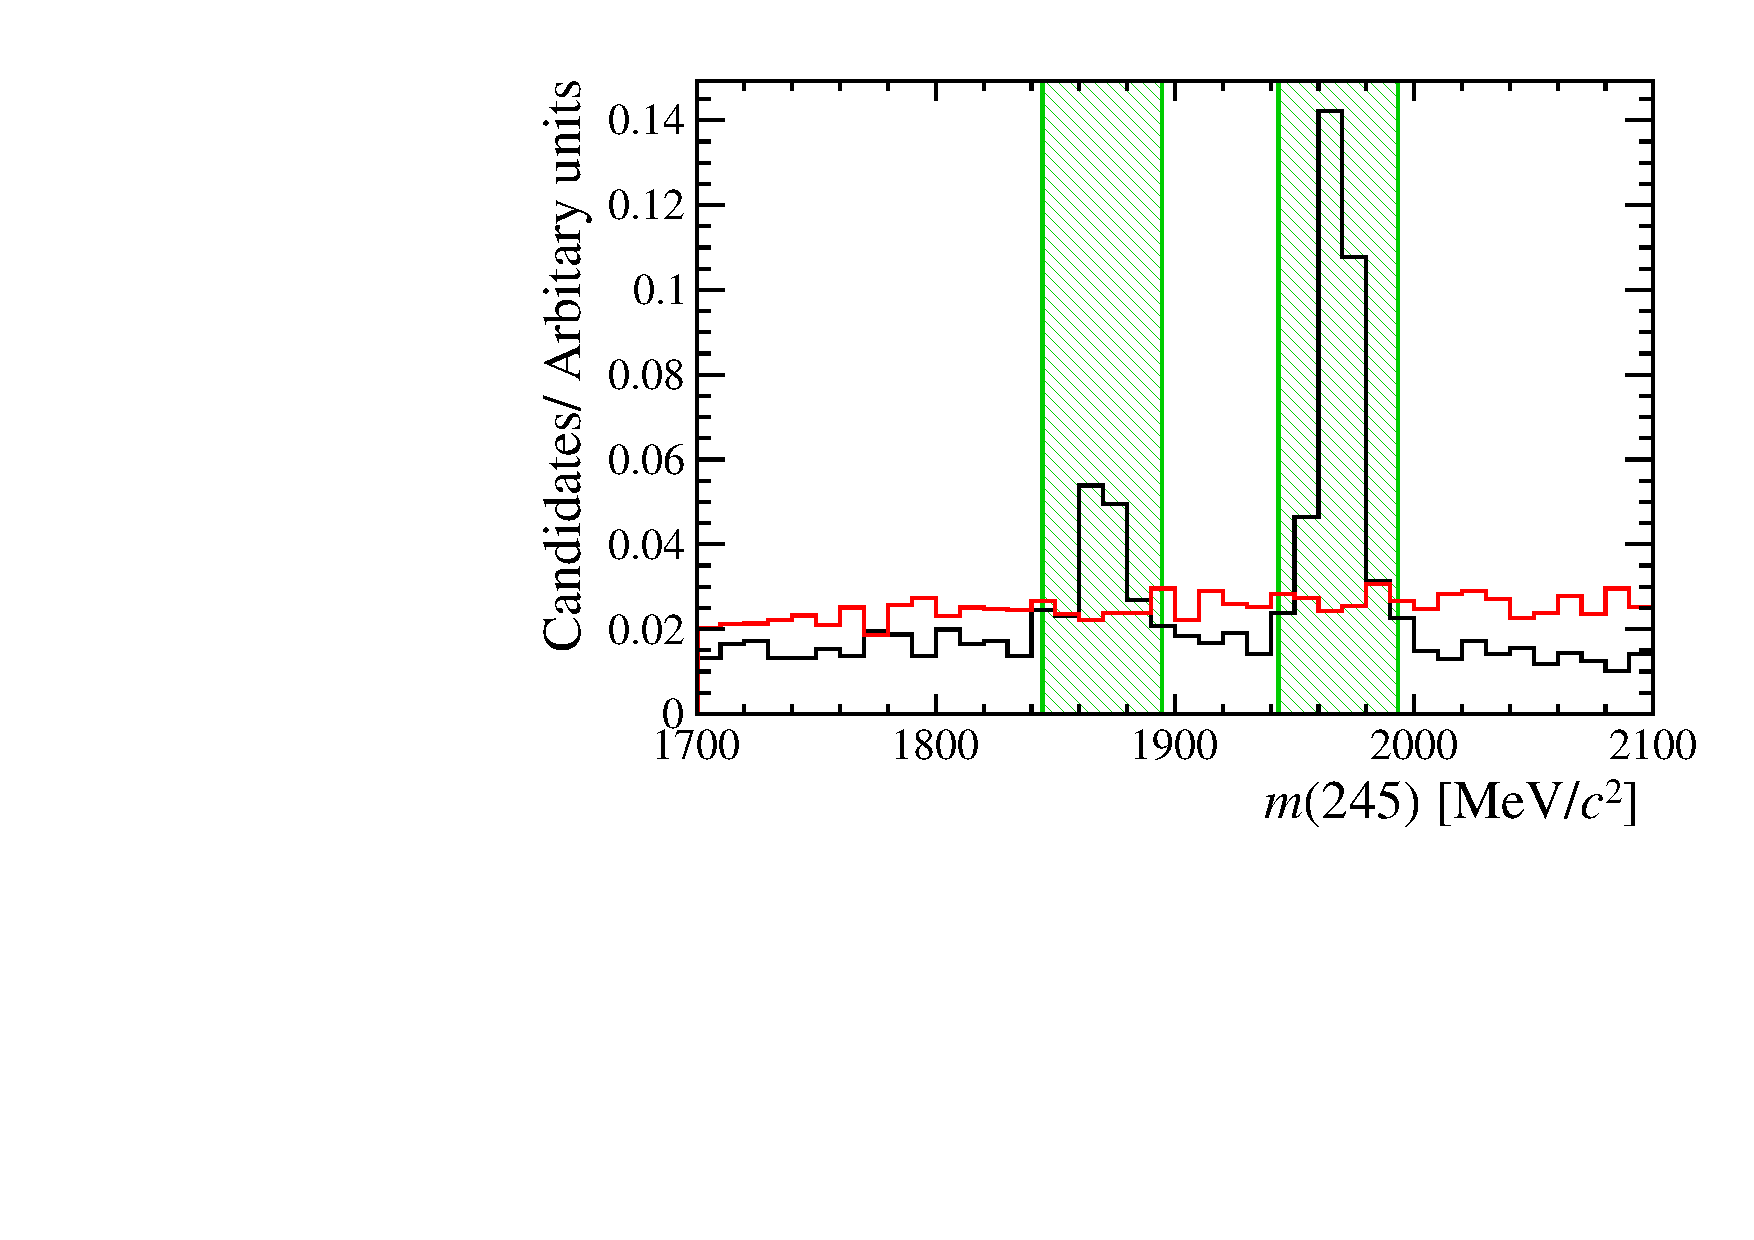
\includegraphics[width=1.0\textwidth]{figs/Selection/Veto_Comparison_B2DsPhi_Ds2PiPiPi_m245.pdf}
      \end{subfigure}
      \begin{subfigure}[t]{0.32\textwidth}
         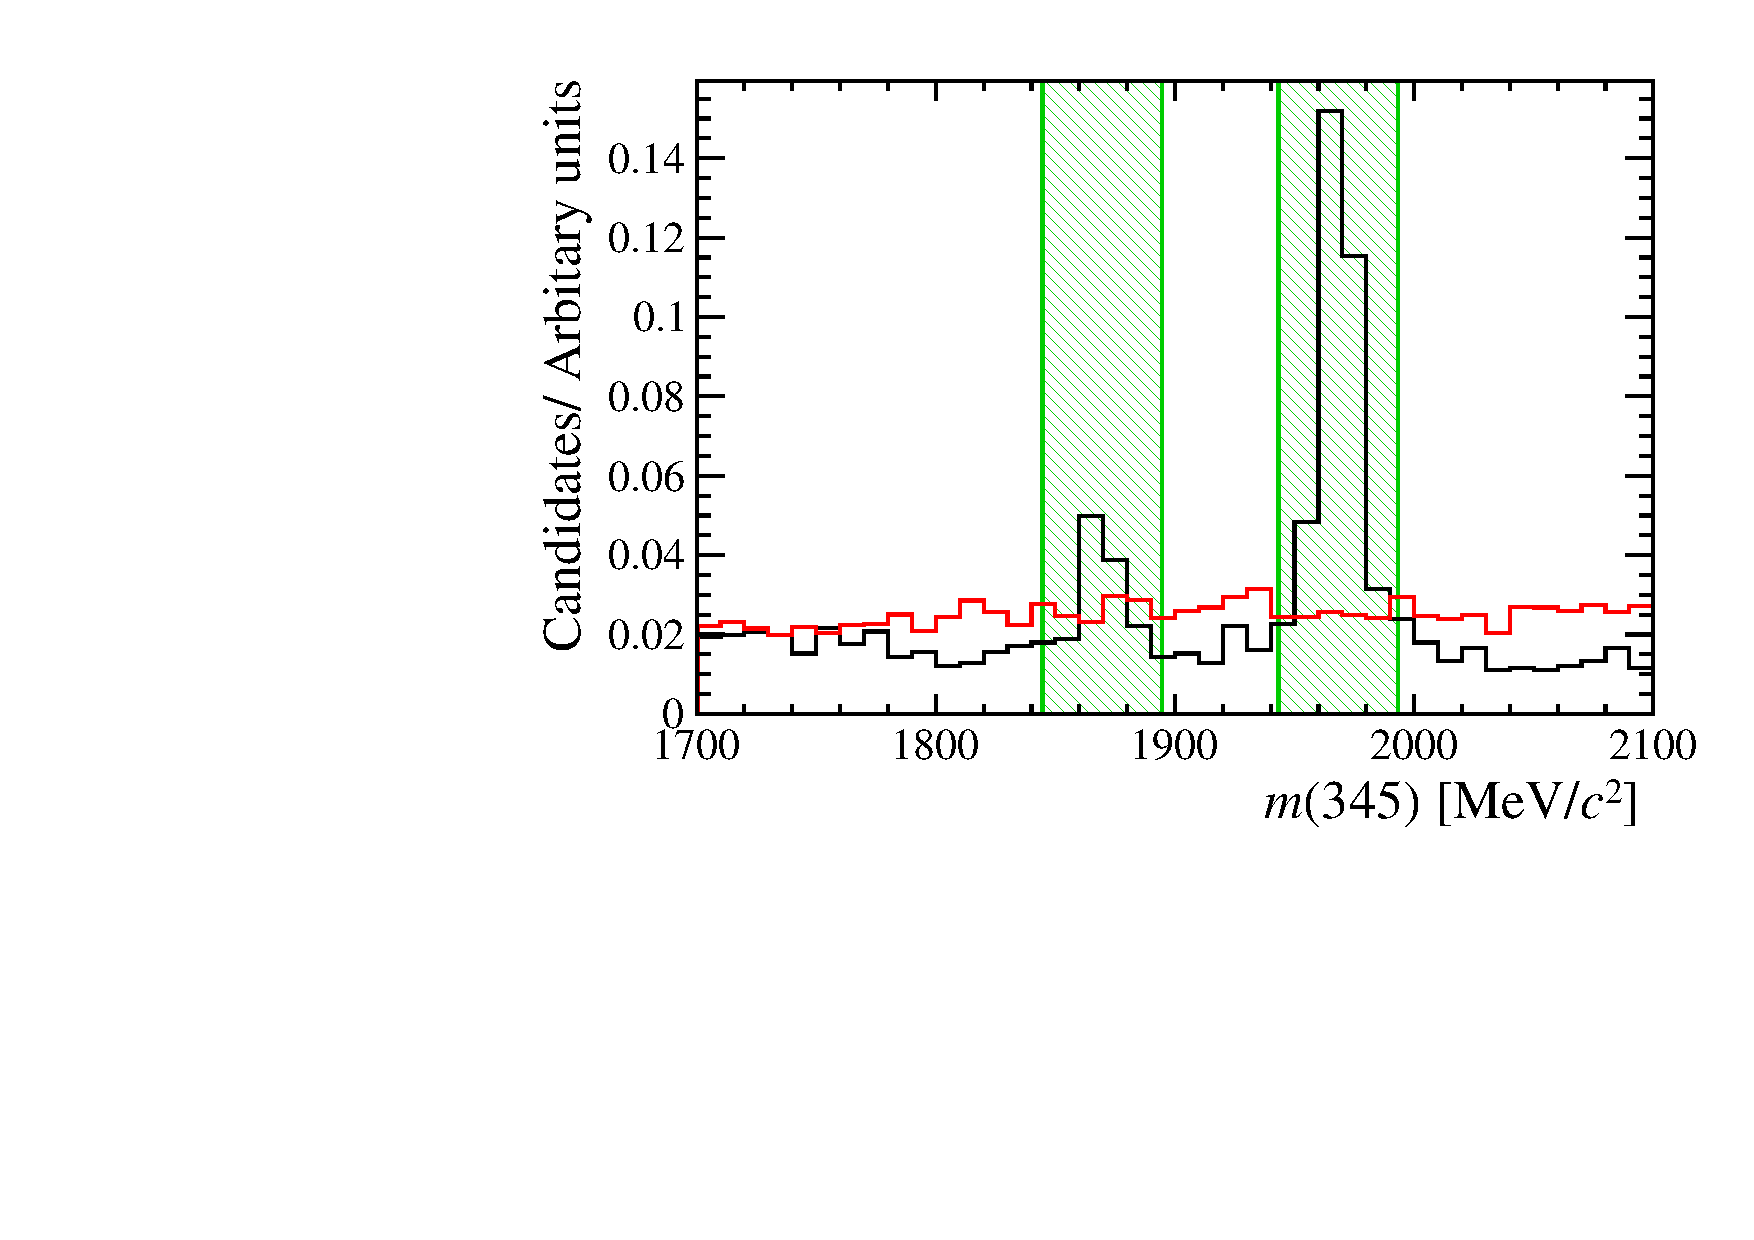
\includegraphics[width=1.0\textwidth]{figs/Selection/Veto_Comparison_B2DsPhi_Ds2PiPiPi_m345.pdf}
      \end{subfigure}
      \caption{\decay{\Bp}{(\decay{\Dsp}{\pip\pim\pip})\phiz}}
   \end{subfigure}
   \begin{subfigure}[t]{1.0\textwidth}
      \centering
      \begin{subfigure}[t]{0.32\textwidth}
         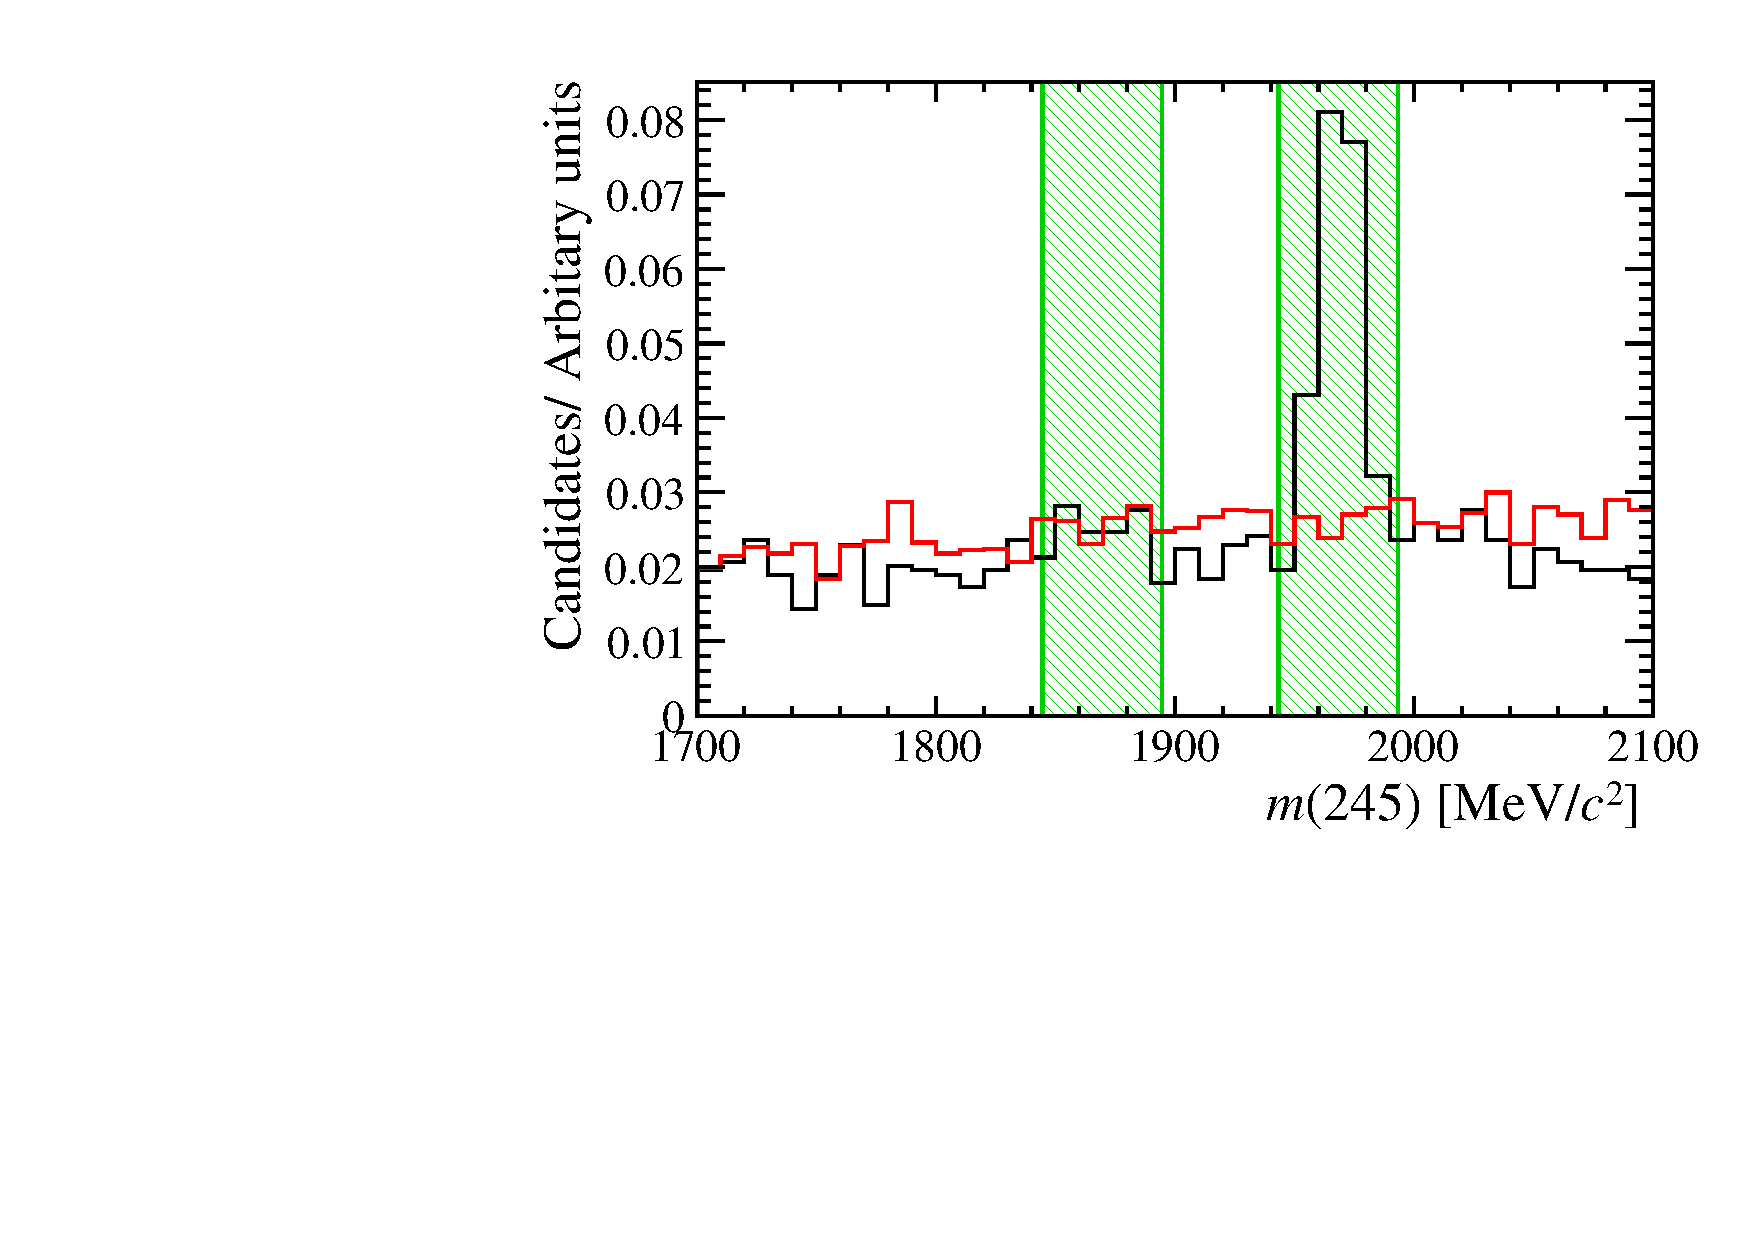
\includegraphics[width=1.0\textwidth]{figs/Selection/Veto_Comparison_B2DsPhi_Ds2KPiPi_m245.pdf}
      \end{subfigure}
      \begin{subfigure}[t]{0.32\textwidth}
         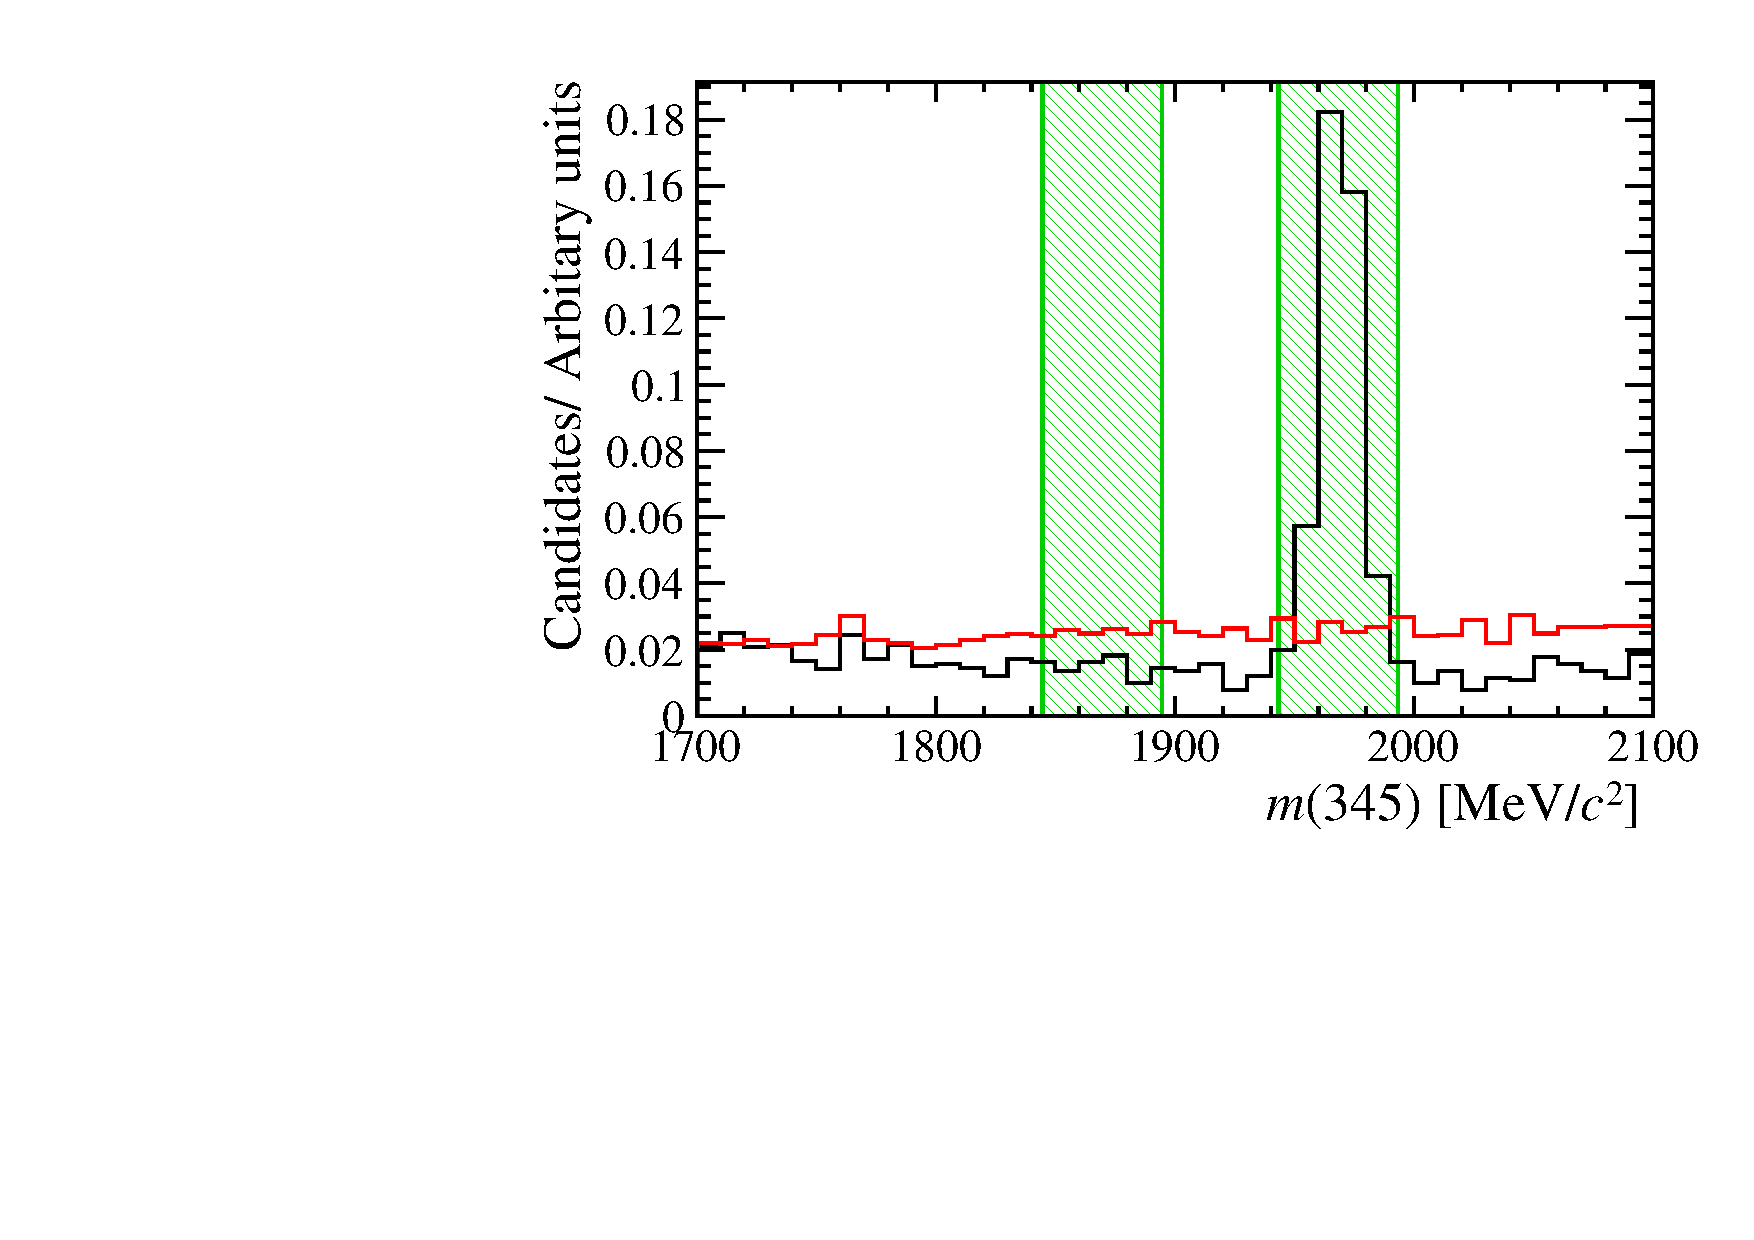
\includegraphics[width=1.0\textwidth]{figs/Selection/Veto_Comparison_B2DsPhi_Ds2KPiPi_m345.pdf}
      \end{subfigure}
      \caption{\decay{\Bp}{(\decay{\Dsp}{\Kp\pim\pip})\phiz}}
   \end{subfigure}

   \caption{Invariant mass distributions for subsets of decay products in data (black) and simulation (red). The green region show the regions removed by the vetoes listed in Sec~\ref{sec:kinematicvetos}.}
   \label{fig:invariantmassvetoes}   
\end{figure}
%%%%%%%%%%%%%%%%%%%%%%%%%%%%%%%%%%%%%%%%%%%%%%%%%%%%%%%%%%


In the search for \decay{\Bp}{\Dsp\Kp\Km} decays the increased size of the $m(\Kp\Km)$ phase-space means more of the combinations of final state particles are susceptible to sharp peaking structure from incorrectly reconstructed backgrounds. Those spectra found to have significant peaking structures are additionally vetoed, as shown in Fig.~\ref{fig:invariantmassvetoes_DsKK}.

\begin{itemize}
\item Vetoes for the mode \decay{\Bp}{(\decay{\Dsp}{\Kp\Km\pip})\Kp\Km}:
\begin{itemize}
\item $|m(\text{1245})- m(\Bs)| > 50\mevcc$
\item $|m(\text{345})- m(\Dsp)| > 25\mevcc$ and $|m(\text{345})- m(\Dp)| > 25\mevcc$
\item $|m(\text{135})- m(\Dsp)| > 25\mevcc$
\item $|m(\text{234})- m(\Dsp)| > 25\mevcc$
\end{itemize}
\end{itemize}

%%%%%%%%%%%%%%%%%%%%%%%%%%%%%%%%%%%%%%%%%%%%%%%%%%%%%%%%%%
\begin{figure}[!h]
   \centering
   \begin{subfigure}[t]{1.0\textwidth}
      \centering
      \begin{subfigure}[t]{0.32\textwidth}
         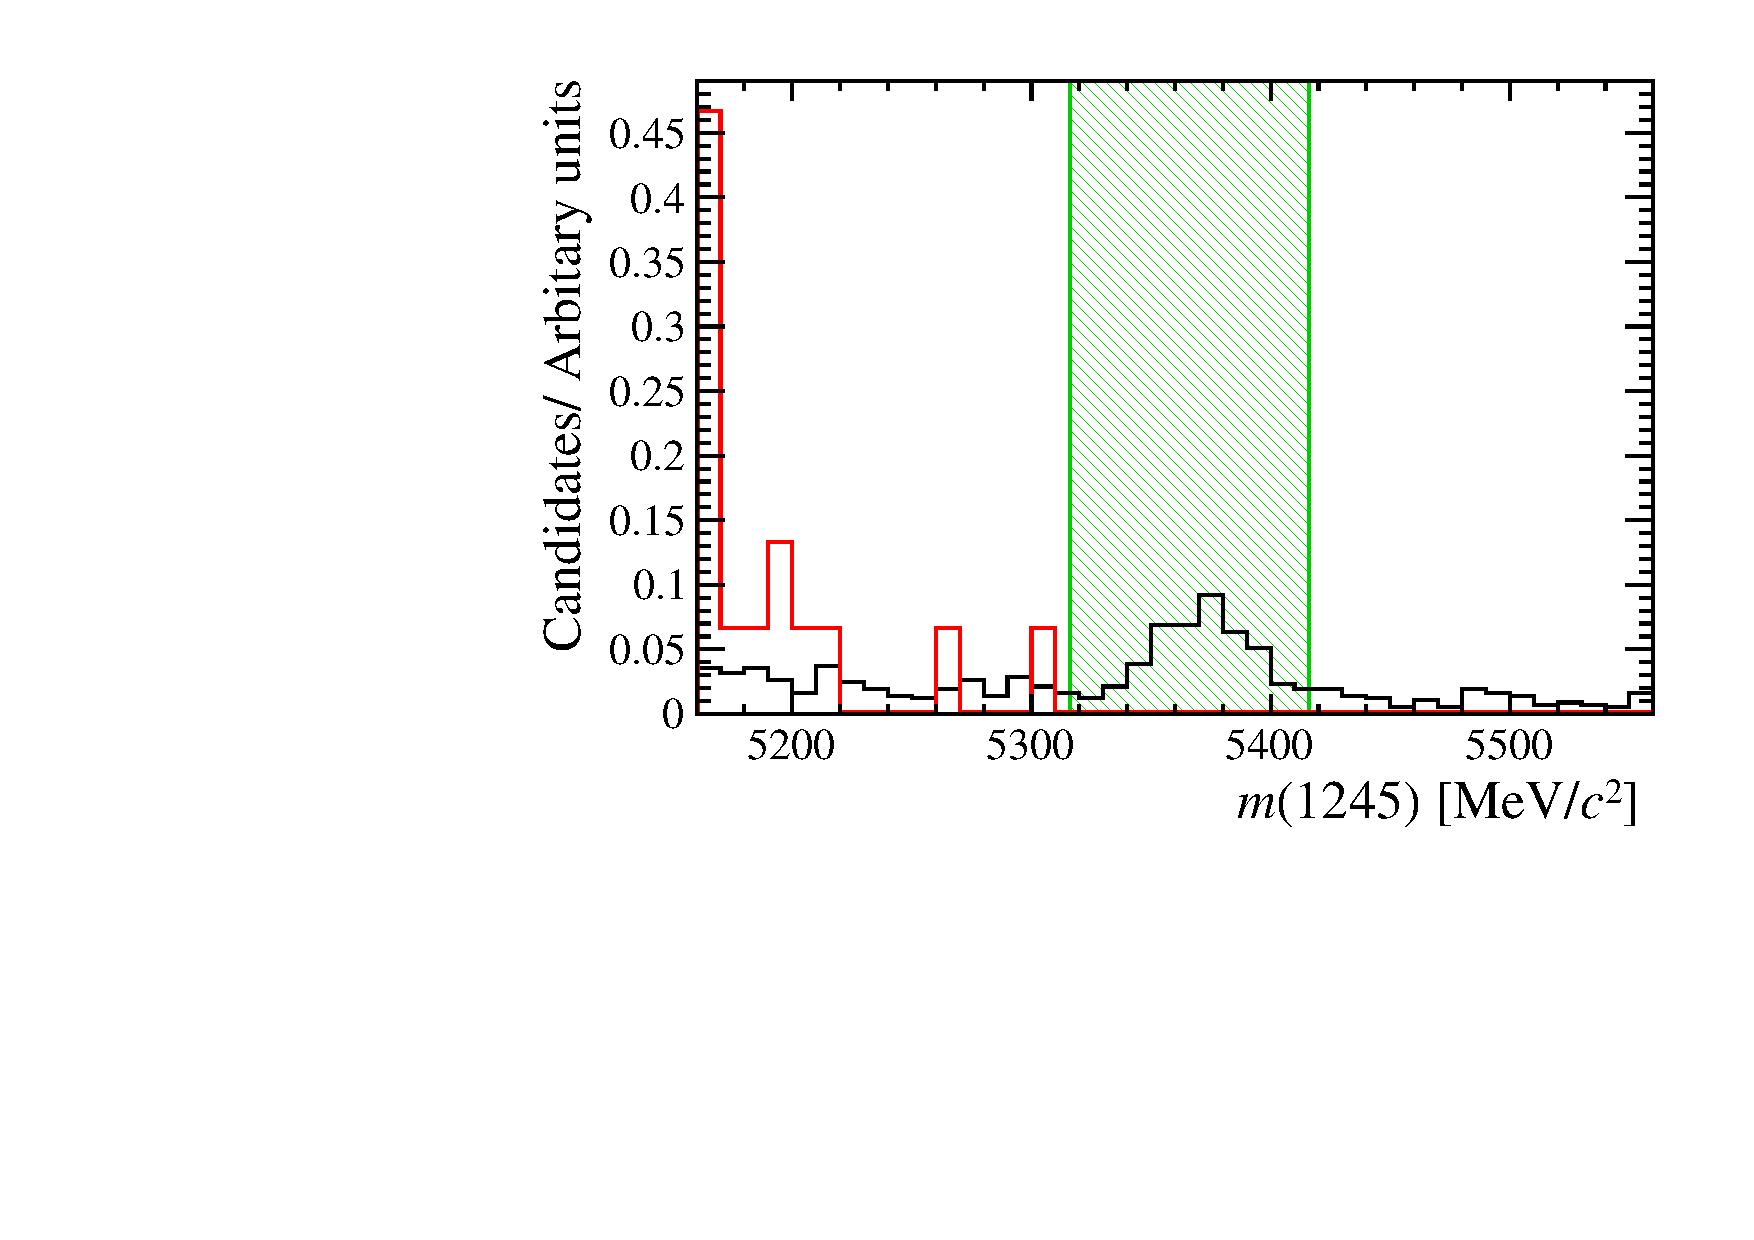
\includegraphics[width=1.0\textwidth]{figs/Selection/Veto_Comparison_B2DsKK_Ds2KKPi_m1245.pdf}
      \end{subfigure}\\
      \begin{subfigure}[t]{0.32\textwidth}
         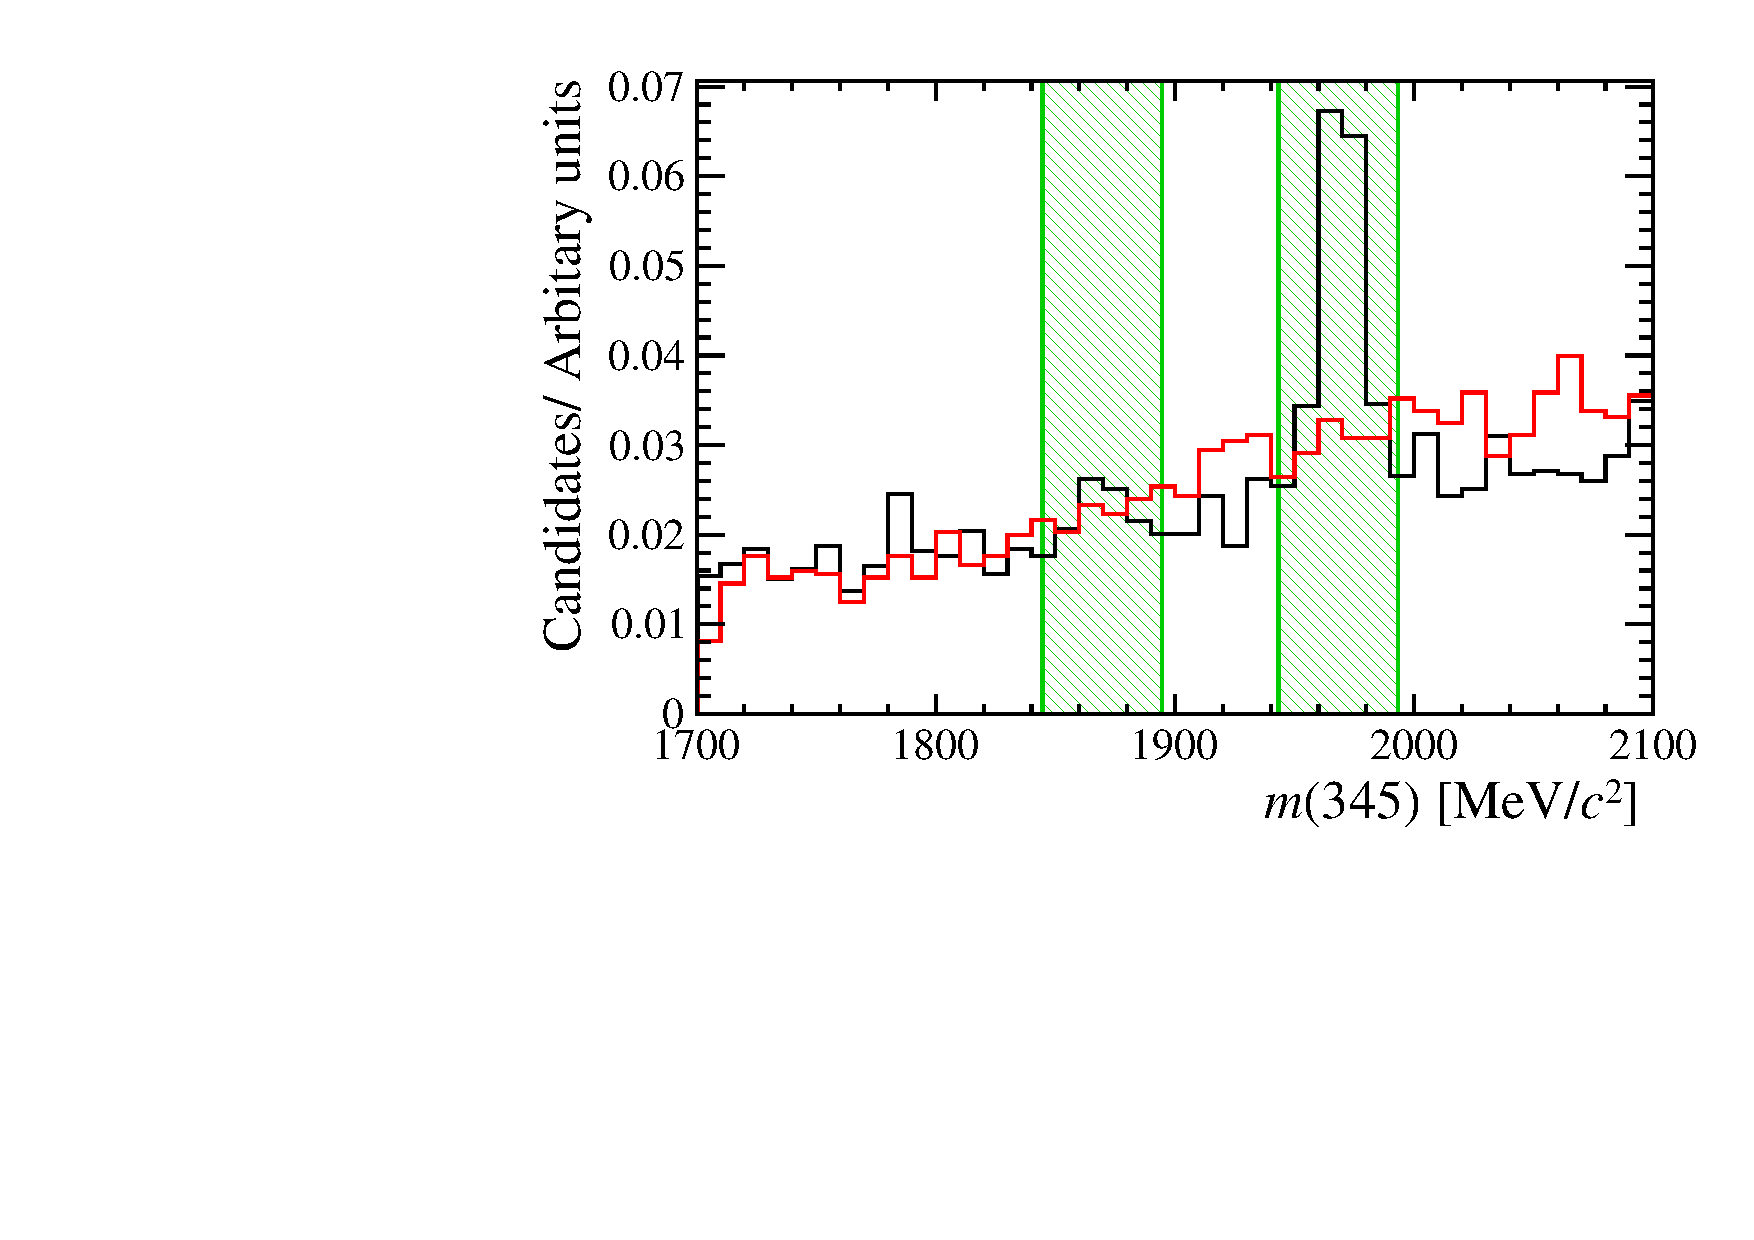
\includegraphics[width=1.0\textwidth]{figs/Selection/Veto_Comparison_B2DsKK_Ds2KKPi_m345.pdf}
      \end{subfigure}
      \begin{subfigure}[t]{0.32\textwidth}
         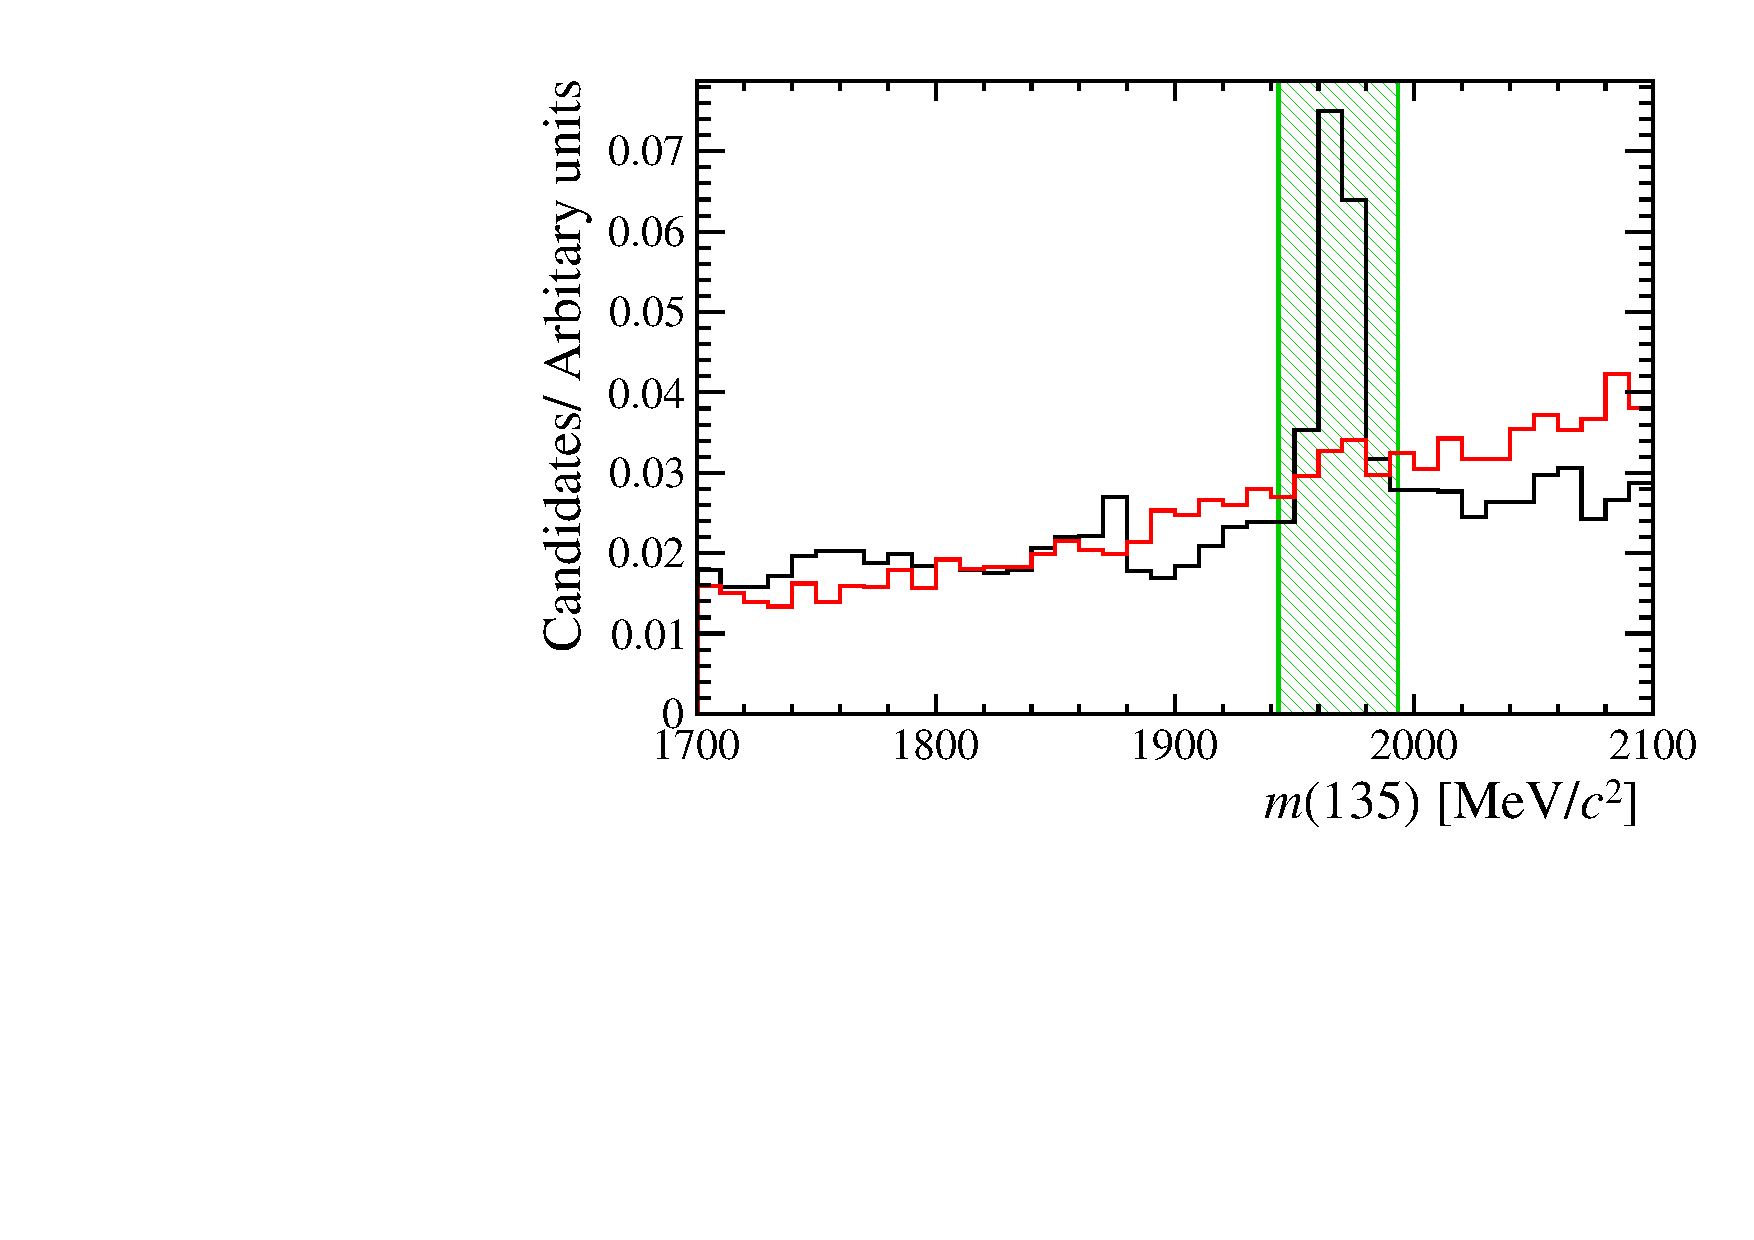
\includegraphics[width=1.0\textwidth]{figs/Selection/Veto_Comparison_B2DsKK_Ds2KKPi_m135.pdf}
      \end{subfigure}
      \begin{subfigure}[t]{0.32\textwidth}
         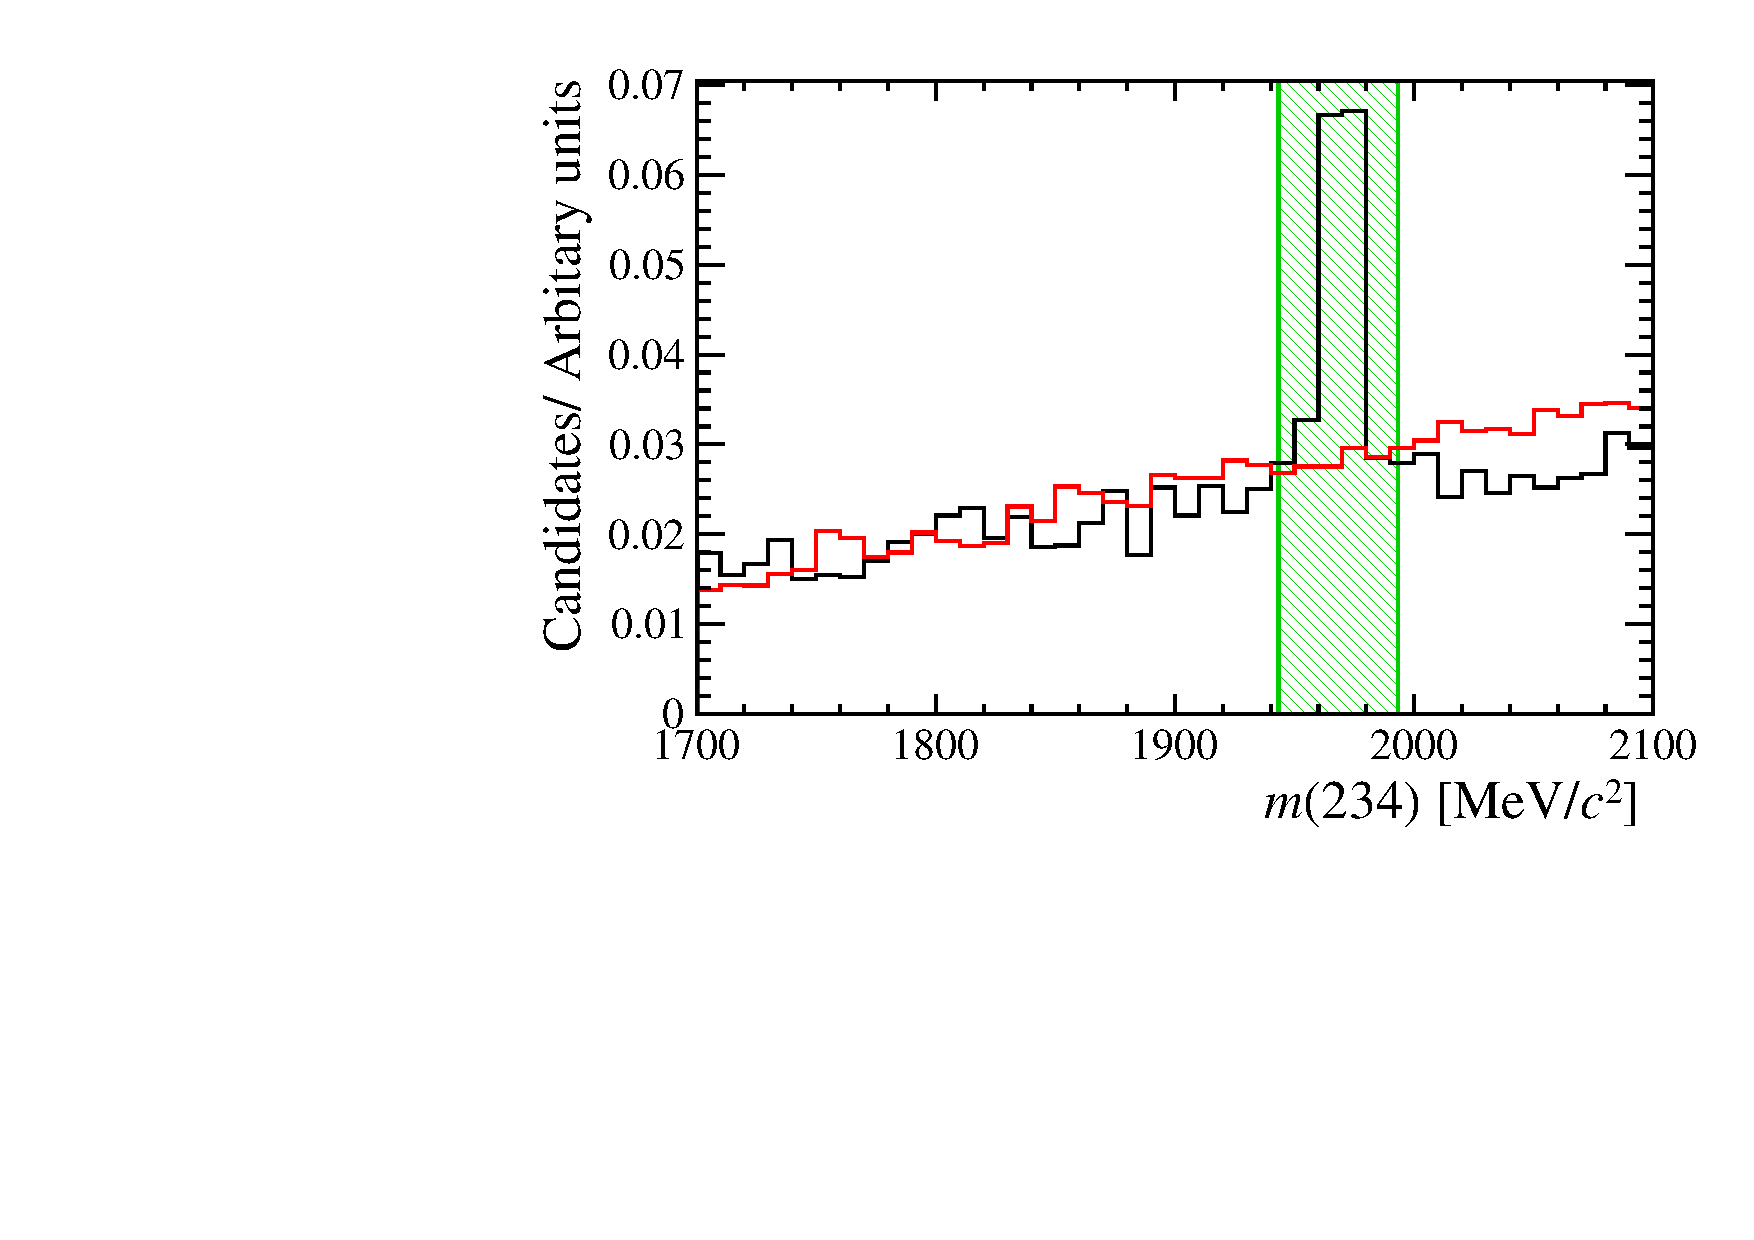
\includegraphics[width=1.0\textwidth]{figs/Selection/Veto_Comparison_B2DsKK_Ds2KKPi_m234.pdf}
      \end{subfigure}
   \end{subfigure}

   \caption{Invariant mass distributions for subsets of decay products for \decay{\Bp}{(\decay{\Dsp}{\Kp\Km\pip})\Kp\Km} decays in data (black) and simulation (red). The green region show the regions removed by the vetoes listed in Sec~\ref{sec:kinematicvetos}.}
   \label{fig:invariantmassvetoes_DsKK}   
\end{figure}
%%%%%%%%%%%%%%%%%%%%%%%%%%%%%%%%%%%%%%%%%%%%%%%%%%%%%%%%%%
 
Another set of vetoes rejects decays where the tracks forming the \Dsp candidate originate from an excited charged charm meson decay, for example $\decay{\Dstarp}{(\decay{\Dz}{h^{+}h'^{-}}) \pip}$. By requiring $\Delta m = m(h^{+}h'^{-}\pip)-m(h^{+}h'^{-}) > 150 \mevcc$ decays of this type are efficiently removed. These are applied to both the signal and normalisation modes for all \Dsp decays. 


\subsection{Normalisation mode veto}
\label{sec:normvetos}

In the search for \decay{\Bp}{\Dsp\Kp\Km} decays, the entire $m(\Kp\Km)$ phasespace is used. This ranges from the \Kp\Km mass threshold at around $990\mevcc$ to the kinematic limit at $m(\Bp) - m(\Dsp) = 3300\mevcc$. This range is wide enough to include the mass of the \Dzb meson, $m(\Dz) = 1864 \mevcc$. Consequently, when inspecting the $m(\Kp\Km)$ spectrum for selected signal candidates there is an excess of events at the \Dz mass. It is necessary to remove these from the signal samples as, unsurprisingly, they result in a peak at the \Bp mass in the $m(\Dsp\Kp\Km)$ spectrum and lead to an incorrect signal yield. As described in Section~\ref{sec:selectionrequirements}, these removed events are used as the normalisation channel for the measurement of \decay{\Bp}{\Dsp\Kp\Km} decays. 
The region affected by the veto $|m(\Kp\Km) - m(\Dzb)| > 25 \mevcc$ is shown in Fig.~\ref{fig:normalisationveto_KK}.

%%%%%%%%%%%%%%%%%%%%%%%%%%%%%%%%%%%%%%%%%%%%%%%%%%%%%%%%%%
\begin{figure}[!h]
   \centering
   \begin{subfigure}[t]{0.49\textwidth}
      \centering
      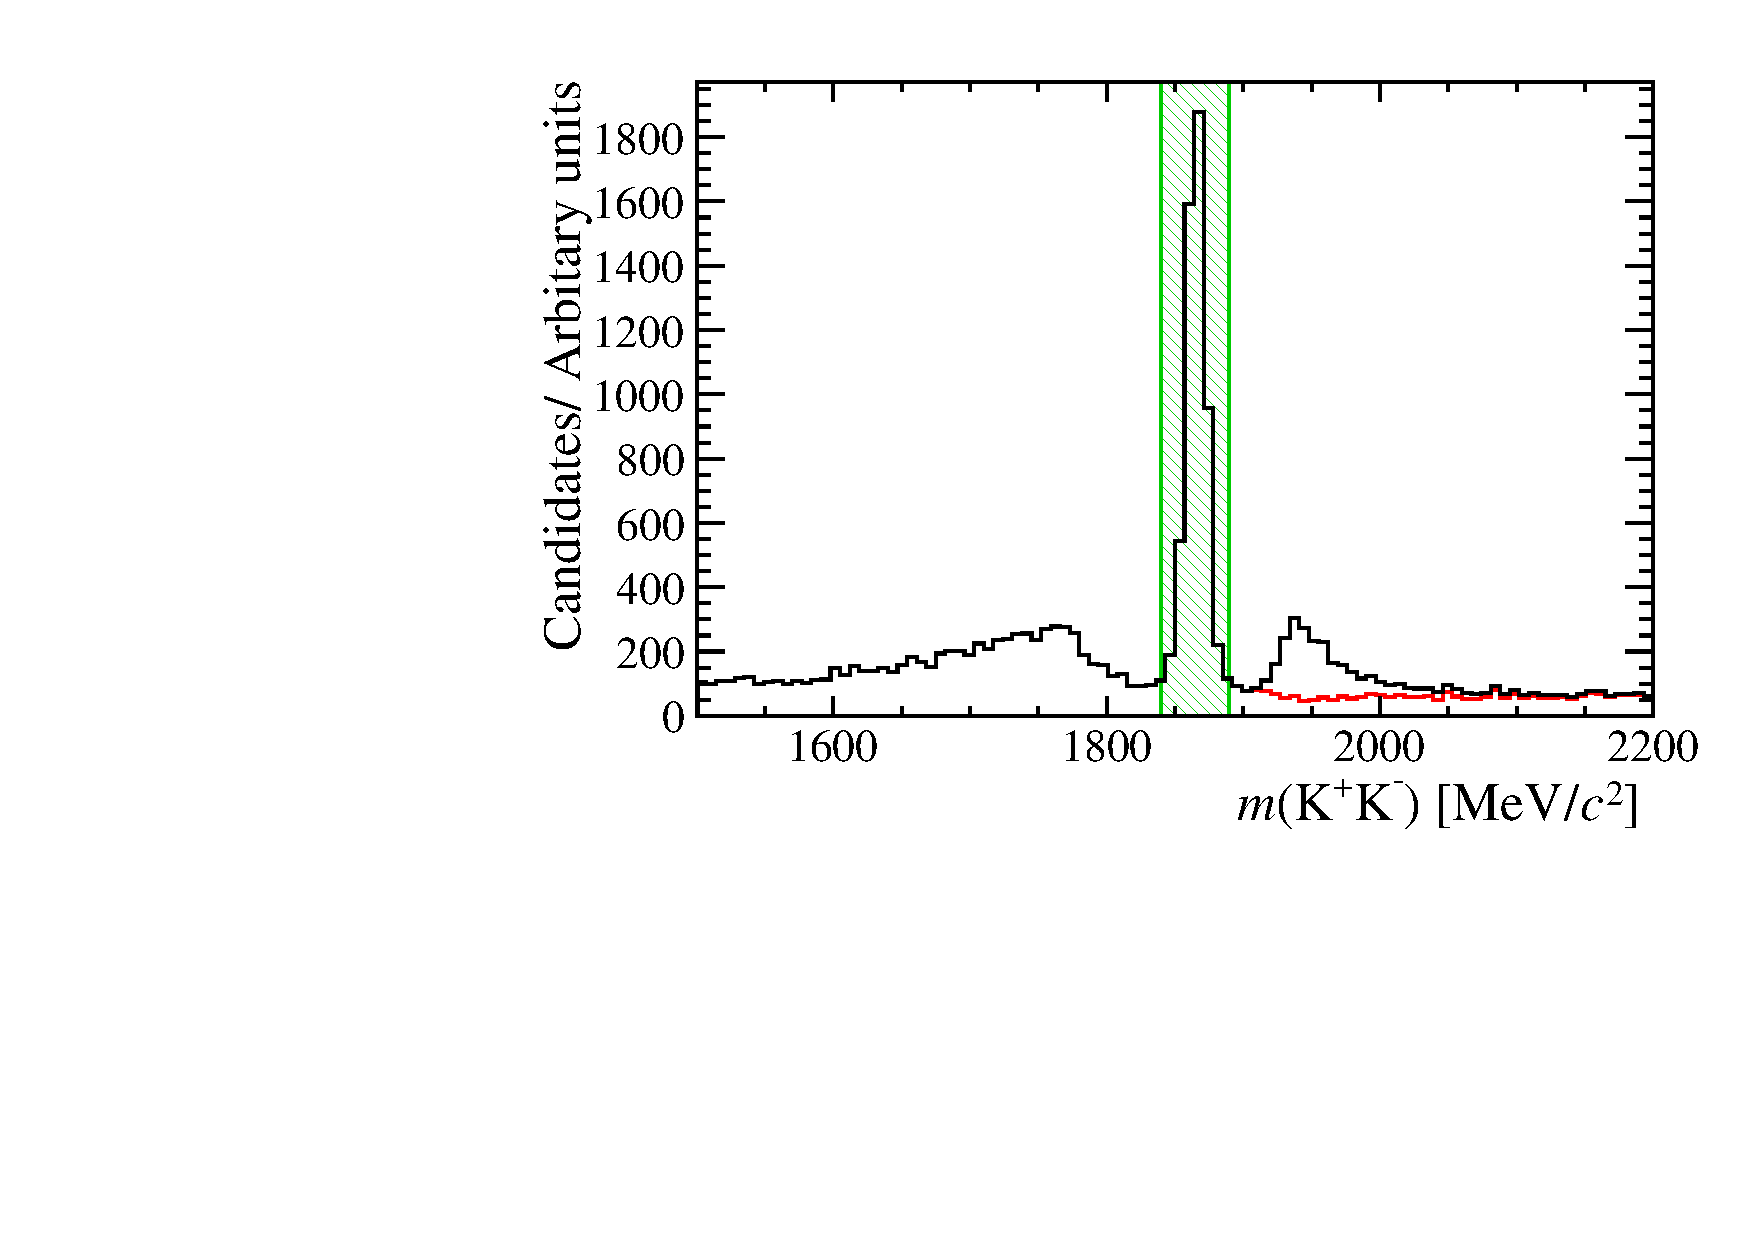
\includegraphics[width=1.0\textwidth]{figs/Selection/D0Veto_Comparison_B2DsKK_Ds2KKPi_Phi_M.pdf}
      \caption{\decay{\Dzb}{\Kp\Km} }
      \label{fig:normalisationveto_KK}
   \end{subfigure}
   \begin{subfigure}[t]{0.49\textwidth}
      \centering
      \includegraphics[width=1.0\textwidth]{figs/Selection/D0Veto_Comparison_B2DsKK_Ds2KKPi_Phi_KPi_M.pdf}
      \caption{\decay{\Dzb}{\Kp\pim} }
      \label{fig:normalisationveto_KPi}
   \end{subfigure}
   \caption{The vetoes applied to remove the normalisation channel \decay{\Bp}{\Dsp\Dzb} from the sample of \decay{\Bp}{\Dsp\Kp\Km} decays. Both the correctly reconstructed \decay{\Dzb}{\Kp\Km} (left) and mis-reconstructed \decay{\Dzb}{\Kp\pim} decays (right) are targeted. The effect of the mis-reconstructed \decay{\Dzb}{\Kp\pim} decay veto on the $m(\Kp\Km)$ distribution is shown in red in the left plot.}
   \label{fig:normalisationveto}   
\end{figure}
%%%%%%%%%%%%%%%%%%%%%%%%%%%%%%%%%%%%%%%%%%%%%%%%%%%%%%%%%%


In addition to the correctly reconstructed normalisation channel, the presence of the incorrectly reconstructed \decay{\Bp}{\Dsp(\decay{\Dzb}{\Kp\pim})} decay is observable in Fig.~\ref{fig:normalisationveto_KK}. This appears as smeared out peak to the right of the \Dzb peak. Although the probability of the \pim meson being misidentified as a \Km meson is low, the branching fraction for \decay{\Dzb}{\Kp\pim} is larger, leading to the observed excess. It is possible, and necessary, to remove this contribution. The \Kp\Km candidates are reconstructed again, swapping the mass hypothesis of the second track from \Km to \pim. The distribution of these candidates in the vicinity of the \Dzb mass is shown in Fig.~\ref{fig:normalisationveto_KPi}. A distinct peak is observed at the \Dzb mass. This contribution is removed by the requirement $|m(\Kp\pim) - m(\Dzb)| > 25 \mevcc$. The effect of this requirement on the $m(\Kp\Km)$ spectrum is shown by the red line in Fig.~\ref{fig:normalisationveto_KK}, which represents the sample with this veto applied. The \decay{\Bp}{\Dsp(\decay{\Dzb}{\Kp\pim})} background is reduced to a negligible level.

Another structure appears to be present to the left of the \Dzb peak in Fig.~\ref{fig:normalisationveto_KK}. This is likely to be due to \decay{\Dzb}{\Kp\Km X} decays in which one or more particles have not been reconstructed. This partially reconstructed background would not peak at the \Bp mass in the $m(\Dsp\Kp\Km)$ spectrum due to the missing particles, therefore no attempt is made to remove this contribution.


\subsection{Multivariate analysis}

Multivariate Analyses (MVAs) are used to help discriminate between genuine \Dsp and \phiz meson decays and combinations of unrelated tracks. 
These MVAs are trained on data using large samples of \B mesons decays which have similar topologies. 
This data-driven approach can benefit from an expanded set of variables that are not perfectly represented in simulation, including track quality and particle identification information, in addition to the widely used kinematic and geometric properties.
The method is based on the approach used in Ref.~\cite{LHCb-PAPER-2012-050}, however the choice of input variables has been optimised and training samples expanded to include Run II data.

The sample of \Dsp mesons is obtained from the relatively abundant \decay{\Bsb}{\Dsp\pim} decay. Similarly, the sample of \phiz mesons is obtained from \decay{\Bs}{\jpsi\phiz} decays. Large, high purity samples are reconstructed using similar requirements to those applied in the selection of signal \Dsp and \phiz mesons.
A sample is selected for each of the \Dsp and \phiz meson decays uses in this analysis, as listed in Table~\ref{tab:mva_modes}. 
The training of separate MVAs for the different \Dsp modes allows the use of particle identification variables that separate kaons and pions to be fully exploited.
The MVA trained using \decay{\Bs}{\jpsi(\decay{\phiz}{\Kp\Km})} decays is used to select both \decay{\phiz}{\Kp}{\Km} and \decay{\Dzb}{\Kp\Km} decays. For the normalisation mode this may be suboptimal, however it ensures the selection of the signal and normalisation channels are almost identical such that the systematic uncertainty in the ratio of efficiencies is minimised.
The samples of \decay{\Bsb}{\Dsp\pim} and \decay{\Bs}{\jpsi\phiz} decays are randomly split into two subsamples. The first is used to train the MVAs and the second is used to determine the efficiency of the selection. To prevent the difference between \phiz and \Dzb decays from affecting the ratio of efficiencies, the normalisation channel MVA efficiency is instead determined from a dedicated sample of \decay{\Dzb}{\Kp\Km} decays as detailed in Table.~\ref{tab:mva_modes}. The \decay{\phiz}{\Kp\Km} MVA is also used to select the \Kp\Km pair in \decay{\Bp}{\Dsp\Kp\Km} decays.
A total of eight MVAs are trained, one for each of the \Dsp and \phiz modes, in both Run I and Run II. Changes to the particle identification variables between the two running periods necessitates separate trainings. 


\begin{table}[h]
\centering
\begin{tabular}{lll}
   \hline
   Sample                    & Mode                       & Use \\ 
   \hline
   \decay{\Bsb}{\Dsp\pim}    & \decay{\Dsp}{\Kp\Km\pip}   & Training, Efficiency \\
   \decay{\Bsb}{\Dsp\pim}    & \decay{\Dsp}{\Kp\pim\pip}  & Training, Efficiency \\
   \decay{\Bsb}{\Dsp\pim}    & \decay{\Dsp}{\pip\pim\pip} & Training, Efficiency \\
   \decay{\Bs}{\jpsi\phiz}   & \decay{\phiz}{\Kp\Km}      & Training, Efficiency \\
   \hline
   \decay{\Bp}{\Dzb\pip}     & \decay{\Dzb}{\Kp\Km}       & Efficiency          \\
   \hline
\end{tabular}

\caption{The decay modes used to train and determine the efficiency of the various MVAs used in this analysis.}
\label{tab:mva_modes}
\end{table}

\subsubsection{Preselection}

Before the samples of \Dsp and \phiz mesons are used to train the MVAs, precautions are taken to ensure the samples are representative of the \decay{\Bp}{\Dsp\phiz} and \decay{\Bp}{\Dsp\Kp\Km} signal decays. The \decay{\Bsb}{\Dsp\pim} and \decay{\Bs}{\jpsi\phiz} decays are selected using a similar procedure to the signal modes. Firstly, \emph{Stripping Lines} reconstruct the candidates. The \decay{\Bsb}{\Dsp\pim} decays are built using the same software module as the signal and normalisation channel. Therefore, the selection requirements for \Dsp candidates in \decay{\Bsb}{\Dsp\pim} decays are identical to those listed for the signal in Table~\ref{tab:strippinglinecuts}.
The \decay{\Bs}{\jpsi\phiz} decays are reconstructed using \decay{\jpsi}{\mup\mun} decays, therefore they are built using a different software module as the final state is not fully hadronic. As such there are some differences in the selection requirements for the \phiz mesons from the two sources. In general the selection requirements for the \decay{\Bs}{\jpsi\phiz} channel are looser as the presence of the muons allows an efficient triggering without the need to make tight selections on the \Kp\Km pair. A direct comparison of the relevant quantities are listed in Table~\ref{tab:strippingrequirments_phi}.

% Phi_P > 7000 && 
% Phi_FDCHI2_OWNPV >15 && 
% Phi_K0_P > 2000 && 
% Phi_K1_P > 2000 && 
% Phi_K0_IPCHI2_OWNPV > 4 && 
% Phi_K1_IPCHI2_OWNPV > 4 &&
% Phi_DIRA_OWNPV>0 && 
% Phi_ENDVERTEX_CHI2<16 && 
% Phi_K0_TRACK_GhostProb<0.4&& 
% Phi_K1_TRACK_GhostProb<0.4 && 
% (Phi_K0_PT+Phi_K1_PT)>1000)

\begin{table}[h]
\centering
\begin{tabular}{ l l l l }
\hline
Particle       & Quantity                       &  Signal                              & Control                                 \\  
\hline
\phiz          & Mass minimum                   &  $870\mevcc$                         & $980\mevcc$ \\ 
               & Mass maximum                   &  $1170\mevcc$                        & $1050\mevcc$ \\ 
               & Transverse Momentum            &  -                                   & $\pt > 500 \mevc$                       \\  
               & Products \pt scalar sum        &  $\sum{|\pt|} > 1000 \mevc$          &  -                                      \\  
               & $\text{DOCA}(\Kp,\Km)$         &  $ < 0.5\mm$     &  -                                      \\  
               & Direction angle                &  $\cos{\theta}>0$                    &  -                                      \\  
               & Vertex quality                 &  $\chi^{2}/N_{\text{DOF}} < 16$      & $\chi^{2}/N_{\text{DOF}} < 25$          \\   
               & Flight distance significance   &  $\chi^{2}_{\text{FD} }  > 16$       &  -                                      \\ 
\hline
\Kpm           & Track quality                  &  $\chi^{2}/N_{\text{DOF}}<4.0$       &  $\chi^{2}/N_{\text{DOF}}<5.0$          \\  
               & Transverse momentum            &  $\pt > 100 \mevc$                   &  -                                      \\  
               & Momentum                       &  $\ptot > 1000 \mevc$                &  -                                      \\  
               & Impact parameter significance  &  $\chi^{2}_{\text{IP}} > 4$          &  -                                      \\  
               & Ghost track probability        &  $P_{\text{Ghost}} < 0.4$            &  -                                      \\
               & Particle identification        &  $\text{PIDK}>-10$                   & $\text{PIDK}>0$                         \\ 
\hline
\end{tabular}

\caption{The \emph{Stripping Line} requirements for \decay{\phiz}{\Kp\Km} candidates in the signal and MVA training (control) mode selection. All requirements are looser for the control channel with the exception of the particle identification requirements.}
\label{tab:strippingrequirments_phi}
\end{table}

The difference in the two selections could be potentially biasing when calculating the efficiency of the MVA, therefore the requirements are tightened on the half of the \decay{\Bs}{\jpsi\phiz} sample used to calculate the efficiency. The looser set of requirements are still used when training the MVA methods to maximise the sample sizes to help prevent overtraining. When training the MVAs the \phiz meson invariant mass sidebands in the \decay{\Bs}{\jpsi\phiz} sample are used as the background sample. It was found that using the tighter set of requirements led to a negligible amount of background candidates, resulting in overtraining. 


The second step of preselection aims to apply the same sequence of requirements to the modes used to train the MVAs as are applied to the signal and normalisation before the MVAs are applied. These are made up of the same trigger, background veto and PID requirements.
For \Dsp candidates from \decay{\Bsb}{\Dsp\pim} decays, the \Bsb meson is required to either be \texttt{TOS} with respect to the \texttt{L0Hadron} trigger or \texttt{TIS} with respect to \texttt{L0Global} as with the signal. The \Bsb candidates are then required to be \texttt{TOS} with respect to the same \hltone and \hlttwo triggers as used with the signal modes.

For the \decay{\Bs}{\jpsi\phiz} candidates, a large fraction are triggered due to the muons from the \jpsi decay. To ensure the sample is reflective of the signal decays the \Bs meson is required to be \texttt{TOS} with respect to the \texttt{L0Hadron} trigger or \texttt{TIS} with respect to \texttt{L0Global}. This effectively excludes events that have been selected solely due to muons initiating the muon hardware trigger. This consequently results in a large decrease in the available statistics.

As shown in Table~\ref{tab:strippingrequirments_phi}, the MVA training mode has tighter particle identification requirements than the signal mode. Particle identification plays a crucial role in the efficacy of the MVA methods, therefore the signal PID requirements for the \phiz meson decay products are tightened accordingly as discussed in Section~\ref{sec:pidrequirements}.

Finally, the same misidentified \D and \Lc hadron vetoes as detailed in Section~\ref{sec:pidvetos} are applied to the \decay{\Bsb}{\Dsp\pim} sample. These help to ensure the samples of \Dsp candidates are free from contamination.


\subsubsection{Background subtraction}
\label{sec:MVAbackgroundsubtraction}
%% Describe fits, sWeights and signal/background samples
In order to use the \decay{\Bs}{\jpsi\phiz} and \decay{\Bsb}{\Dsp\pim} samples to train MVAs, background subtracted distributions must be obtained for the variables used to discriminate the signal from backgrounds.  Firstly, unbinned extended maximum likelihood fits are performed to the \Dsp and \phiz invariant mass distribution in order to determine the yield of \Dsp and \phiz candidates respectively. 
Maximum likelihood fits determine the values of the signal and background yields for which the given data set was most likely. The likelihood, $\mathcal{L}$, is constructed from the probability density functions (PDFs) for the fit model, $F(m,\vec{p})$, for each entry $i$ in the data set. The PDF for each entry is evaluated at the corresponding value of the invariant mass, $m = m_{i}$, such that $\mathcal{L}$ is just a function of the PDF parameters, $\vec{p}$,
\begin{equation}
\mathcal{L}(\vec{p}) = \prod_{i}^{N} F(m=m_{i},\vec{p}).
\end{equation}

The maximum value of $\mathcal{L}(\vec{p})$ is achieved for the set of PDF parameters for which the data was most likely. 
It is computationally beneficial to instead compute the negative log-likelihood (NLL) rather than the likelihood directly, as addition is less intensive than multiplication. The NLL,
\begin{equation}
-\log\mathcal{L}(\vec{p}) = -\sum_{i}^{N} \log F(m=m_{i},\vec{p}),
\end{equation}
is then minimised with respect to the PDF parameters.

This likelihood can be \emph{extended} to allow the total yield attributed to the PDF to be determined as a parameter as well. This is nessesary to determine the yields of both signal and background contributions ($n_{\text{S}}$ and $n_{\text{B}}$).
The likelihood is multiplied by the Poisson probability density for measuring $n = n_{\text{S}} + n_{\text{B}}$ events, 
\begin{equation}
\mathcal{L}(n,\vec{p}) = \frac{n^{N}e^{-n}}{N!}\prod_{i}^{N} F(m=m_{i},\vec{p}) = \frac{e^{-n}}{N!}\prod_{i}^{N} n F(m=m_{i},\vec{p}).
\end{equation}

The extended NLL becomes 
\begin{equation}
-\log\mathcal{L}(n,\vec{p}) = -\sum_{i}^{N} \log n F(m=m_{i},\vec{p}) + n + \log N!.
\end{equation}
The $\log N!$ term can be ignored as it is a constant.
The fit model is constructed from signal and background contributions 
\begin{equation}
n F(m| n_{\text{S}},n_{\text{B}},\vec{p'},\vec{p''}) = n_{\text{S}} f(m|\vec{p'}) + n_{\text{B}} g(m|\vec{p''}),
\end{equation}
where $n_{\text{S}}$ and $n_{\text{B}}$ are the signal and background yields, $f$ and $g$ are the PDFs for the signal and background respectively, and $\vec{p'}$ and $\vec{p''}$ represent the parameters controlling the PDF shapes.

After the extended maximum likelihood fits have been performed and the yields established, the subtraction of candidates attributed to the background component is performed using the \sPlot technique~\cite{Pivk:2004ty}.
The \sPlot method assigns weights for each species in the fit model, namely signal and background. These are assigned to each event in the data set and are only dependent on the value of the fitted variable, in this case \phiz or \Dsp mass. When plotting other, uncorrelated variables and weighting each event accordingly, the contribution from each component in the fit can be extracted. 

%% Fit model
For both \decay{\Bs}{\jpsi\phiz} and \decay{\Bsb}{\Dsp\pim} decays, simple fit models are found to be sufficient when performing the \sPlot technique. For each mode the signal components are modelled with a single Gaussian probability density function
\begin{equation}
f(m|\mu,\sigma) = \frac{1}{\sqrt{2\pi\sigma^{2}}} \times e^{-\frac{(m-\mu)^{2}}{2\sigma^{2}}}, 
\end{equation}
where $\mu$ and $\sigma$ are the mean and width of the Gaussian distribution and $m$ is the observable invariant mass. The parameters $\mu$ and $\sigma$ are allowed to vary freely.
The background contributions to the \decay{\phiz}{\Kp\Km} decays are modelled using a Chebychev polynomial with two degrees of freedom
\begin{equation}
g(m|a,b) = a\times(2m^{2}-1) + b\times m + 1,
\end{equation}
where $a$ and $b$ are parameters that can vary freely and $m$ is the observable invariant mass. 
The \phiz meson mass is close to the threshold for \Kp\Km pair production so this parametrisation has sufficient freedom to successfully  model the increasing background shape.
The background contribution to all three \Dsp decays are modelled using exponential functions with a single degree of freedom controlling the effective slope
\begin{equation}
g(m|c) = e^{-m\times c},
\end{equation}
where $c$ is a freely varying parameter and $m$ is the observable invariant mass.
The fits to the \phiz and \Dsp meson masses in the \decay{\Bs}{\jpsi\phiz} and \decay{\Bsb}{\Dsp\pim} samples are performed separately for each year of data taking and polarity of the \lhcb dipole magnet. These distributions are shown in Fig.~\ref{fig:mvatrainingsamples} for each of the \phiz and \Dsp decay modes.
The yields of candidates in each of the subsamples are tabulated in Table~\ref{table:mva_training_yields}, along with the totals for each mode. 


%%%%%%%%%%%%%%%%%%%%%%%%%%%%%%%%%%%%%%%%%%%%%%%%%%%%%%%%%%
\begin{figure}[!h]
   \centering
   \begin{subfigure}[t]{0.4\textwidth}
      \centering
      \includegraphics[width=1.0\textwidth]{figs/Selection/Fit_Data_Bs2JpsiPhi_Jpsi2MuMu_Phi2KK_2016_MagDown.pdf}
      \caption{\decay{\phiz}{\Kp\Km} MagDown}
   \end{subfigure}
   \begin{subfigure}[t]{0.4\textwidth}
      \centering
      \includegraphics[width=1.0\textwidth]{figs/Selection/Fit_Data_Bs2JpsiPhi_Jpsi2MuMu_Phi2KK_2016_MagUp.pdf}
      \caption{\decay{\phiz}{\Kp\Km} MagUp}
   \end{subfigure}\\
   \begin{subfigure}[t]{0.4\textwidth}
      \centering
      \includegraphics[width=1.0\textwidth]{figs/Selection/Fit_Data_Bs02DsPi_Ds2KKPi_2016_MagDown_PreSel.pdf}
      \caption{\decay{\Dsp}{\Kp\Km\pip} MagDown}
   \end{subfigure}
   \begin{subfigure}[t]{0.4\textwidth}
      \centering
      \includegraphics[width=1.0\textwidth]{figs/Selection/Fit_Data_Bs02DsPi_Ds2KKPi_2016_MagUp_PreSel.pdf}
      \caption{\decay{\Dsp}{\Kp\Km\pip} MagUp}
   \end{subfigure}
   \begin{subfigure}[t]{0.4\textwidth}
      \centering
      \includegraphics[width=1.0\textwidth]{figs/Selection/Fit_Data_Bs02DsPi_Ds2PiPiPi_2016_MagDown_PreSel.pdf}
      \caption{\decay{\Dsp}{\pip\pim\pip} MagDown}
   \end{subfigure}
   \begin{subfigure}[t]{0.4\textwidth}
      \centering
      \includegraphics[width=1.0\textwidth]{figs/Selection/Fit_Data_Bs02DsPi_Ds2PiPiPi_2016_MagUp_PreSel.pdf}
      \caption{\decay{\Dsp}{\pip\pim\pip} MagUp}
   \end{subfigure}
   \begin{subfigure}[t]{0.4\textwidth}
      \centering
      \includegraphics[width=1.0\textwidth]{figs/Selection/Fit_Data_Bs02DsPi_Ds2KPiPi_2016_MagDown_PreSel.pdf}
      \caption{\decay{\Dsp}{\Kp\pim\pip} MagDown}
   \end{subfigure}
   \begin{subfigure}[t]{0.4\textwidth}
      \centering
      \includegraphics[width=1.0\textwidth]{figs/Selection/Fit_Data_Bs02DsPi_Ds2KPiPi_2016_MagUp_PreSel.pdf}
      \caption{\decay{\Dsp}{\Kp\pim\pip} MagUp}
   \end{subfigure}
   \caption{Unbinned maximum likelihood fit to \decay{\Bs}{\jpsi\phiz} (top) and \decay{\Bsb}{\Dsp\pim} (bottom three rows) candidates. These distributions correspond to just the 2016 data samples. Slight discrepancies are observed as a result of the simplified fit model in the top two plots.}
   \label{fig:mvatrainingsamples}
\end{figure}


%%%%%%%%%%%%%%%%%%%%%%%%%%%%%%%%%%%%%%%%%%%%%%%%%%%%%%%%%%
\begin{table}[!h]
   \centering
      \begin{tabular}{ll S[table-format=6.0(4)] S[table-format=6.0(4)] S[table-format=7.0(4)]}
         \hline
         Mode                       & Year   & {MagDown}          & {MagUp}           & {Total} \\ 
         \hline                                                
         \decay{\phiz}{\Kp\Km}      & 2011   & 3190 \pm 170     &   2120 \pm 140  &    \\
                                    & 2012   & 5800 \pm 200     &   5540 \pm 200  &     \\
                                    & 2015   & 2240 \pm 110     &   1640 \pm 100  &     \\
                                    & 2016   & 11200 \pm 300    &   11100 \pm 300 & 42830 \pm 600    \\
         \hline                                                
         \decay{\Dsp}{\Kp\Km\pip}   & 2011   & 97100  \pm 500   & 68600  \pm 400  &     \\
                                    & 2012   & 216600 \pm 800   & 212800 \pm 800  &     \\
                                    & 2015   & 68600  \pm 400   & 43400  \pm 300  &     \\
                                    & 2016   & 321400 \pm 900   & 310800 \pm 900  & 1339300 \pm 1900    \\
         \hline                                                
         \decay{\Dsp}{\pip\pim\pip} & 2011   & 24300 \pm 500    &   17100 \pm 400 &      \\
                                    & 2012   & 57700 \pm 800    &   56500 \pm 900 &     \\
                                    & 2015   & 20400 \pm 500    &   13100 \pm 400 &     \\
                                    & 2016   & 99200 \pm 1200   &  92100 \pm 1200 & 380400 \pm 2300    \\
         \hline                                                
         \decay{\Dsp}{\Kp\pim\pip}  & 2011   & 13200 \pm 600    & 9500  \pm 400   &     \\
                                    & 2012   & 29300 \pm 900    & 29300 \pm 900   &     \\
                                    & 2015   & 10000 \pm 500    & 6200  \pm 400   &     \\
                                    & 2016   & 47800 \pm 1200   & 44200 \pm 1100  & 189500 \pm 2300    \\
         \hline
      \end{tabular}
      \caption{Yields of the samples used to train data-driven MVAs. The total yields are summed over all years and both magnet polarities.}
      \label{table:mva_training_yields}
   
\end{table}
%%%%%%%%%%%%%%%%%%%%%%%%%%%%%%%%%%%%%%%%%%%%%%%%%%%%%%%%%%

\subsubsection{Input variables}


%% Discussion of input variables
The MVA method is trained using a large set of variables chosen to help discriminate between the signals of interest and combinations of unrelated tracks. These variables include the properties of the \Kpm or \pipm decay products as well as those of the \phiz or \Dsp candidate itself. Many of the quantities are the same as those previously defined in Section.~\ref{sec:selectionrequirements}. The additional parameters relate to the track quality and particle identification information and are defined as follows:

\begin{description}
\item \textbf{Track matching quality, $\chi^{2}_{\text{TRKMATCH}}$}: this parameter is an key component of the pattern recognition software that matches the \velo and tracking station track sections together to form \emph{long} tracks. It quantifies the quality of the track matching.

\item \textbf{\velo track quality, $\chi^{2}_{\text{TRKVELO}}$}: this quantifies the quality of the track fit using just the hits in the \velo.  


\item \textbf{Kaon, proton, pion and ghost probabilities, ProbNN$x$ ($x\in[K,\pi,\proton,\text{ghost}]$)}: these variables are an alternative form of \emph{Particle Identification} variables in addition to those already discussed in Section~\ref{sec:pidrequirements}. Each ProbNN$x$ variable acts as the probability for the reconstructed track to be of the species $x$. These variables are the responses of Artificial Neural Networks trained to differentiate between the various particle types using a large number of inputs from different sub-detectors. The trainings use simulated samples of signal and background decays and have been retuned between Run~I and Run~II to reflect the difference in the detector configuration. Four of the available ProbNN$x$ variables are used in this analysis. Three of these identify kaons, protons and pions. The last aims to identify ghost tracks, similar to the $P_{\text{Ghost}}$ variable already discussed. 
\end{description}

The variables used in the \phiz meson MVA are listed in Table~\ref{tab:mvavars_phi}. Some of the variables are input into the MVA training algorithm as their logarithm, rather than the variable directly. These variables tend to be rapidly increasing in at certain values, so using the logarithm aids visualisation. A total of 24 variables are used in this MVA.

When training the \phiz meson MVA, the flight distance significance is not included as an input variable. This MVA is used to select both \phiz and \Dzb mesons which are likely to have different flight distance significance distributions as a result of their different lifetimes. 


\begin{table}[h]
   \centering
      \begin{tabular}{ l l l c c}

         \hline
         Particle       & Description                    & Quantity                             & \Dsp MVA      & \phiz MVA    \\    
         \hline
         \phiz/\Dsp     & Momentum                       &  \ptot                               & \checkmark    & \checkmark   \\  
                        & Transverse Momentum            &  \pt                                 & \checkmark    & \checkmark   \\  
                        & Vertex quality                 &  $\log_{10}(\chi^{2}_{\text{VXT}})$  & \checkmark    & \checkmark   \\  
                        & Impact parameter significance  &  $\log_{10}(\chi^{2}_{\text{IP}})$   & \checkmark    & \checkmark   \\    
                        & Flight distance significance   &  $\log_{10}(\chi^{2}_{\text{FD}})$   & \checkmark    & -            \\    
         \hline
         \Kpm           & Momentum                       &  \ptot                               & \checkmark    & \checkmark   \\  
                        & Transverse momentum            &  \pt                                 & \checkmark    & \checkmark   \\ 
                        & Longitudinal momentum          &  \pz                                 & \checkmark    & -            \\
                        & Impact parameter significance  &  $\log_{10}(\chi^{2}_{\text{IP}})$   & \checkmark    & \checkmark   \\    
                        & Track quality                  &  $\chi^{2}_{\text{TRK}}$             & \checkmark    & \checkmark   \\    
                        & Velo track quality             &  $\chi^{2}_{\text{TRKVELO}}$         & \checkmark    & -            \\    
                        & Track matching quality         &  $\chi^{2}_{\text{TRKMATCH}}$        & \checkmark    & \checkmark   \\    
                        & Kaon probability               &  ProbNNk                             & \checkmark    & \checkmark   \\    
                        & Proton probability             &  ProbNNp                             & \checkmark    & \checkmark   \\    
                        & Pion probability               &  ProbNNpi                            & \checkmark    & \checkmark   \\    
                        & Ghost probability              &  ProbNNghost                         & \checkmark    & \checkmark   \\    
         \hline
      \end{tabular}
   
   \caption{Discriminating variables used to train the \phiz and \Dsp MVAs. Poorly discriminating variables are removed from the \phiz MVA to prevent overtraining. The flight distance significance is remove as the MVA is applied to both \phiz and \Dzb candidates.}
   \label{tab:mvavars_phi}
\end{table}
 
The variables used in the \Dsp MVA are also listed in Table~\ref{tab:mvavars}. These are largely very similar to those used for the \phiz meson MVA, however it also includes the \Dsp meson's flight distance significance as, unlike the \phiz meson, the \Dsp meson decays displaced from its production vertex. A total of 35 variables are used in these MVAs.



% \begin{table}[h]
%    \centering
%       \begin{tabular}{ l l l}

%          \hline
%          Particle       & Description                    & Quantity                          \\    
%          \hline
%          \Dsp           & Momentum                       &  \ptot                            \\  
%                         & Transverse Momentum            &  \pt                              \\  
%                         & Vertex quality                 &  $\log_{10}(\chi^{2}_{\text{VXT}})$    \\  
%                         & Impact parameter significance  &  $\log_{10}(\chi^{2}_{\text{IP}})$     \\    
%                         & Flight distance significance   &  $\log_{10}(\chi^{2}_{\text{FD}})$     \\    
%          \hline
%          \Kpm, \pipm    & Momentum                       &  \ptot                            \\  
%                         & Transverse momentum            &  \pt                              \\
%                         & Impact parameter significance  &  $\log_{10}(\chi^{2}_{\text{IP}})$     \\    
%                         & Track quality                  &  $\chi^{2}_{\text{TRK}}$          \\    
%                         & Velo track quality             &  $\chi^{2}_{\text{TRKVELO}}$      \\    
%                         & Track matching quality         &  $\chi^{2}_{\text{TRKMATCH}}$     \\    
%                         & Kaon probability               &  ProbNNk                          \\    
%                         & Proton probability             &  ProbNNp                          \\    
%                         & Pion probability               &  ProbNNpi                         \\    
%                         & Ghost probability              &  ProbNNghost                      \\    
%          \hline
%       \end{tabular}
   
%    \caption{Discriminating variables used to train the \Dsp MVAs.}
%    \label{tab:mvavars_ds}
% \end{table}


When training the MVA methods, the variables are ranked according to their discrimination power. Examples of these ranking are shown for the Run~II, \decay{\phiz}{\Kp\Km} MVA and Run~II, \decay{\Dsp}{\Kp\Km\pip} MVA in Table~\ref{tab:mvarank_dsandphi}. It can be seen that for both the \Dsp and \phiz meson MVAs that the kaon particle identification variable and various $\log_{10}(\chi^{2}_{\text{IP}})$ variables are the most discriminating.

\begin{table}[h]
\centering
\scalebox{1.0}{
\begin{tabular}{ c l c | c l c}

\hline 

\multicolumn{3}{c|}{\decay{\Dsp}{\Kp\Km\pip}}                 & \multicolumn{3}{c}{\decay{\phiz}{\Kp\Km}}                       \\
Rank & Variable                             & Importance (\%) & Rank & Variable                           & Importance (\%)      \\
\hline
 1 & \Kp ProbNNk                            & $7.6$ &  1 & \Kp ProbNNk                                & $6.0$\\
 2 & \Km ProbNNk                            & $6.0$ &  2 & \phiz $\log_{10}(\chi^{2}_{\text{IP}})$    & $6.0$\\
 3 & \Kp $\log_{10}(\chi^{2}_{\text{IP}})$  & $5.5$ &  3 & \Km $\log_{10}(\chi^{2}_{\text{IP}})$      & $6.0$\\
 4 & \pip $\log_{10}(\chi^{2}_{\text{IP}})$ & $5.0$ &  4 & \phiz $\log_{10}(\chi^{2}_{\text{VTX}})$   & $5.8$\\
 5 & \Kp \ptot                              & $4.3$ &  5 & \Km ProbNNpi                               & $5.8$\\
 6 & \Dsp $\log_{10}(\chi^{2}_{\text{IP}})$ & $4.1$ &  6 & \Kp $\log_{10}(\chi^{2}_{\text{IP}})$      & $5.8$\\
 7 & \pip \pt                               & $4.0$ &  7 & \Kp ProbNNghost                            & $5.4$\\
 8 & \Kp \pt                                & $3.9$ &  8 & \Km ProbNNk                                & $5.4$\\
 9 & \pip ProbNNpi                          & $3.9$ &  9 & \Kp $\chi^{2}_{\text{TRK}}$                & $5.6$\\
10 & \Dsp $\log_{10}(\chi^{2}_{\text{FD}})$ & $3.8$ & 10 & \Km $\chi^{2}_{\text{TRK}}$                & $5.2$\\
11 & \Km $\log_{10}(\chi^{2}_{\text{IP}})$  & $3.7$ & 11 & \Kp ProbNNpi                               & $5.2$\\
12 & \Dsp $\log_{10}(\chi^{2}_{\text{VTX}})$& $3.0$ & 12 & \Km ProbNNghost                            & $5.0$\\
13 & \Km \ptot                              & $2.8$ & 13 & \Kp ProbNNp                                & $4.5$\\
14 & \Kp ProbNNp                            & $2.8$ & 14 & \Km ProbNNp                                & $4.4$\\
15 & \Km ProbNNp                            & $2.7$ & 15 & \Kp $\chi^{2}_{\text{TRKMATCH}}$           & $4.3$\\
% 16 & \pip ProbNNghost                   & $2.623$ & 16 & \Km $\chi^{2}_{\text{TRKMATCH}}$     & $3.977\times 10^{-2}$\\
% 17 & \Kp ProbNNghost                    & $2.593$ & 17 & \Km \pt                              & $3.437\times 10^{-2}$\\
% 18 & \Dsp \pt                           & $2.543$ & 18 & \Kp \pt                              & $3.012\times 10^{-2}$\\
% 19 & \Kp ProbNNpi                       & $2.525$ & 19 & \phiz PT                             & $2.400\times 10^{-2}$\\
% 20 & \Km \pt                            & $2.355$ & 20 & \phiz P                              & $1.792\times 10^{-2}$\\
% 21 & \Dsp \ptot                         & $2.327$ & 21 & \Km \pz                              & $1.397\times 10^{-2}$\\
% 22 & \Km ProbNNpi                       & $2.226$ & 22 & \Km \ptot                            & $1.387\times 10^{-2}$\\
% 23 & \pip \ptot                         & $2.083$ & 23 & \Kp \pz                              & $1.245\times 10^{-2}$\\
% 24 & \pip ProbNNp                       & $1.849$ & 24 & \Kp \ptot                            & $1.218\times 10^{-2}$\\
% 25 & \pip ProbNNk                       & $1.793$ \\
% 26 & \Km ProbNNghost                    & $1.607$ \\
% 27 & \pip $\chi^{2}_{\text{TRKVELO}}$   & $1.589$ \\
% 28 & \Km $\chi^{2}_{\text{TRK}}$        & $1.588$ \\
% 29 & \pip $\chi^{2}_{\text{TRKMATCH}}$  & $1.548$ \\
% 30 & \Kp $\chi^{2}_{\text{TRK}}$        & $1.522$ \\
% 31 & \Km $\chi^{2}_{\text{TRKMATCH}}$   & $1.442$ \\
% 32 & \pip $\chi^{2}_{\text{TRK}}$       & $1.433$ \\
% 33 & \Kp $\chi^{2}_{\text{TRKVELO}}$    & $1.184$ \\
% 34 & \Kp $\chi^{2}_{\text{TRKMATCH}}$   & $1.176$ \\
% 35 & \Km $\chi^{2}_{\text{TRKVELO}}$    & $8.818\times10^{-3}$ \\
\hline
\end{tabular}
}
\caption{Ranking of variables for the 15 highest ranked variables used to train the \decay{\Dsp}{\Kp\Km\pip} (left) and \decay{\phiz}{\Kp\Km} (right) Run~II MVAs.}
\label{tab:mvarank_dsandphi}
\end{table}


%%%%%%%%%%%%%%%%%%%%%%%%%%%%%%%%%%%%%%%%%%%%%%%%%%%%%%%%%%
\begin{figure}[!h]
   \centering
   \begin{subfigure}[t]{0.22\textwidth}
      \centering
      \includegraphics[width=1.0\textwidth]{figs/Selection/Phi_BDT_Var_Ds2KKPi_Phi_P.pdf}
   \end{subfigure}
   \begin{subfigure}[t]{0.22\textwidth}
      \centering
      \includegraphics[width=1.0\textwidth]{figs/Selection/Phi_BDT_Var_Ds2KKPi_Phi_PT.pdf}
   \end{subfigure}
   \begin{subfigure}[t]{0.22\textwidth}
      \centering
      \includegraphics[width=1.0\textwidth]{figs/Selection/Phi_BDT_Var_Ds2KKPi_log10_Phi_ENDVERTEX_CHI2.pdf}
   \end{subfigure}
   \begin{subfigure}[t]{0.22\textwidth}
      \centering
      \includegraphics[width=1.0\textwidth]{figs/Selection/Phi_BDT_Var_Ds2KKPi_log10_Phi_IPCHI2_OWNPV.pdf}
   \end{subfigure}
   \begin{subfigure}[t]{0.22\textwidth}
      \centering
      \includegraphics[width=1.0\textwidth]{figs/Selection/Phi_BDT_Var_Ds2KKPi_Phi_K0_P.pdf}
   \end{subfigure}
   \begin{subfigure}[t]{0.22\textwidth}
      \centering
      \includegraphics[width=1.0\textwidth]{figs/Selection/Phi_BDT_Var_Ds2KKPi_Phi_K1_P.pdf}
   \end{subfigure}
   \begin{subfigure}[t]{0.22\textwidth}
      \centering
      \includegraphics[width=1.0\textwidth]{figs/Selection/Phi_BDT_Var_Ds2KKPi_Phi_K0_PT.pdf}
   \end{subfigure}
   \begin{subfigure}[t]{0.22\textwidth}
      \centering
      \includegraphics[width=1.0\textwidth]{figs/Selection/Phi_BDT_Var_Ds2KKPi_Phi_K1_PT.pdf}
   \end{subfigure}
   \begin{subfigure}[t]{0.22\textwidth}
      \centering
      \includegraphics[width=1.0\textwidth]{figs/Selection/Phi_BDT_Var_Ds2KKPi_Phi_K0_PZ.pdf}
   \end{subfigure}
   \begin{subfigure}[t]{0.22\textwidth}
      \centering
      \includegraphics[width=1.0\textwidth]{figs/Selection/Phi_BDT_Var_Ds2KKPi_Phi_K1_PZ.pdf}
   \end{subfigure}
   \begin{subfigure}[t]{0.22\textwidth}
      \centering
      \includegraphics[width=1.0\textwidth]{figs/Selection/Phi_BDT_Var_Ds2KKPi_log10_Phi_K0_IPCHI2_OWNPV.pdf}
   \end{subfigure}
   \begin{subfigure}[t]{0.22\textwidth}
      \centering
      \includegraphics[width=1.0\textwidth]{figs/Selection/Phi_BDT_Var_Ds2KKPi_log10_Phi_K1_IPCHI2_OWNPV.pdf}
   \end{subfigure}
   \begin{subfigure}[t]{0.22\textwidth}
      \centering
      \includegraphics[width=1.0\textwidth]{figs/Selection/Phi_BDT_Var_Ds2KKPi_Phi_K0_MC15TuneV1_ProbNNk.pdf}
   \end{subfigure}
   \begin{subfigure}[t]{0.22\textwidth}
      \centering
      \includegraphics[width=1.0\textwidth]{figs/Selection/Phi_BDT_Var_Ds2KKPi_Phi_K1_MC15TuneV1_ProbNNk.pdf}
   \end{subfigure}
   \begin{subfigure}[t]{0.22\textwidth}
      \centering
      \includegraphics[width=1.0\textwidth]{figs/Selection/Phi_BDT_Var_Ds2KKPi_Phi_K0_MC15TuneV1_ProbNNp.pdf}
   \end{subfigure}
   \begin{subfigure}[t]{0.22\textwidth}
      \centering
      \includegraphics[width=1.0\textwidth]{figs/Selection/Phi_BDT_Var_Ds2KKPi_Phi_K1_MC15TuneV1_ProbNNp.pdf}
   \end{subfigure}
   \begin{subfigure}[t]{0.22\textwidth}
      \centering
      \includegraphics[width=1.0\textwidth]{figs/Selection/Phi_BDT_Var_Ds2KKPi_Phi_K0_MC15TuneV1_ProbNNpi.pdf}
   \end{subfigure}
   \begin{subfigure}[t]{0.22\textwidth}
      \centering
      \includegraphics[width=1.0\textwidth]{figs/Selection/Phi_BDT_Var_Ds2KKPi_Phi_K1_MC15TuneV1_ProbNNpi.pdf}
   \end{subfigure}
   \begin{subfigure}[t]{0.22\textwidth}
      \centering
      \includegraphics[width=1.0\textwidth]{figs/Selection/Phi_BDT_Var_Ds2KKPi_Phi_K0_MC15TuneV1_ProbNNghost.pdf}
   \end{subfigure}
   \begin{subfigure}[t]{0.22\textwidth}
      \centering
      \includegraphics[width=1.0\textwidth]{figs/Selection/Phi_BDT_Var_Ds2KKPi_Phi_K1_MC15TuneV1_ProbNNghost.pdf}
   \end{subfigure}
   \begin{subfigure}[t]{0.22\textwidth}
      \centering
      \includegraphics[width=1.0\textwidth]{figs/Selection/Phi_BDT_Var_Ds2KKPi_Phi_K0_TRACK_CHI2NDOF.pdf}
   \end{subfigure}
   \begin{subfigure}[t]{0.22\textwidth}
      \centering
      \includegraphics[width=1.0\textwidth]{figs/Selection/Phi_BDT_Var_Ds2KKPi_Phi_K1_TRACK_CHI2NDOF.pdf}
   \end{subfigure}
   \begin{subfigure}[t]{0.22\textwidth}
      \centering
      \includegraphics[width=1.0\textwidth]{figs/Selection/Phi_BDT_Var_Ds2KKPi_Phi_K0_TRACK_MatchCHI2.pdf}
   \end{subfigure}
   \begin{subfigure}[t]{0.22\textwidth}
      \centering
      \includegraphics[width=1.0\textwidth]{figs/Selection/Phi_BDT_Var_Ds2KKPi_Phi_K1_TRACK_MatchCHI2.pdf}
   \end{subfigure}
   \caption{Distributions of MVA training variables in the signal (blue) and background (red) samples for the Run~II \decay{\phiz}{\Kp\Km} MVA.}
   \label{fig:mvatrainingvariables_phi}   
\end{figure}
%%%%%%%%%%%%%%%%%%%%%%%%%%%%%%%%%%%%%%%%%%%%%%%%%%%%%%%%%%



%%%%%%%%%%%%%%%%%%%%%%%%%%%%%%%%%%%%%%%%%%%%%%%%%%%%%%%%%%
\begin{figure}[!h]
   \centering
   \begin{subfigure}[t]{0.22\textwidth}
      \centering
      \includegraphics[width=1.0\textwidth]{figs/Selection/Ds_BDT_Var_Ds2KKPi_D_P.pdf}
   \end{subfigure}
   \begin{subfigure}[t]{0.22\textwidth}
      \centering
      \includegraphics[width=1.0\textwidth]{figs/Selection/Ds_BDT_Var_Ds2KKPi_D_PT.pdf}
   \end{subfigure}
   \begin{subfigure}[t]{0.22\textwidth}
      \centering
      \includegraphics[width=1.0\textwidth]{figs/Selection/Ds_BDT_Var_Ds2KKPi_log10_D_ENDVERTEX_CHI2.pdf}
   \end{subfigure}
   \begin{subfigure}[t]{0.22\textwidth}
      \centering
      \includegraphics[width=1.0\textwidth]{figs/Selection/Ds_BDT_Var_Ds2KKPi_log10_D_IPCHI2_OWNPV.pdf}
   \end{subfigure}
   \begin{subfigure}[t]{0.22\textwidth}
      \centering
      \includegraphics[width=1.0\textwidth]{figs/Selection/Ds_BDT_Var_Ds2KKPi_log10_D_FDCHI2_OWNPV.pdf}
   \end{subfigure}
   \begin{subfigure}[t]{0.22\textwidth}
      \centering
      \includegraphics[width=1.0\textwidth]{figs/Selection/Ds_BDT_Var_Ds2KKPi_D_K0_P.pdf}
   \end{subfigure}
   \begin{subfigure}[t]{0.22\textwidth}
      \centering
      \includegraphics[width=1.0\textwidth]{figs/Selection/Ds_BDT_Var_Ds2KKPi_D_K1_P.pdf}
   \end{subfigure}
   \begin{subfigure}[t]{0.22\textwidth}
      \centering
      \includegraphics[width=1.0\textwidth]{figs/Selection/Ds_BDT_Var_Ds2KKPi_D_P_P.pdf}
   \end{subfigure}
   \begin{subfigure}[t]{0.22\textwidth}
      \centering
      \includegraphics[width=1.0\textwidth]{figs/Selection/Ds_BDT_Var_Ds2KKPi_D_K0_PT.pdf}
   \end{subfigure}
   \begin{subfigure}[t]{0.22\textwidth}
      \centering
      \includegraphics[width=1.0\textwidth]{figs/Selection/Ds_BDT_Var_Ds2KKPi_D_K1_PT.pdf}
   \end{subfigure}
   \begin{subfigure}[t]{0.22\textwidth}
      \centering
      \includegraphics[width=1.0\textwidth]{figs/Selection/Ds_BDT_Var_Ds2KKPi_D_P_PT.pdf}
   \end{subfigure}
   \begin{subfigure}[t]{0.22\textwidth}
      \centering
      \includegraphics[width=1.0\textwidth]{figs/Selection/Ds_BDT_Var_Ds2KKPi_log10_D_K0_IPCHI2_OWNPV.pdf}
   \end{subfigure}
   \begin{subfigure}[t]{0.22\textwidth}
      \centering
      \includegraphics[width=1.0\textwidth]{figs/Selection/Ds_BDT_Var_Ds2KKPi_log10_D_K1_IPCHI2_OWNPV.pdf}
   \end{subfigure}
   \begin{subfigure}[t]{0.22\textwidth}
      \centering
      \includegraphics[width=1.0\textwidth]{figs/Selection/Ds_BDT_Var_Ds2KKPi_log10_D_P_IPCHI2_OWNPV.pdf}
   \end{subfigure}
   \begin{subfigure}[t]{0.22\textwidth}
      \centering
      \includegraphics[width=1.0\textwidth]{figs/Selection/Ds_BDT_Var_Ds2KKPi_D_K0_MC15TuneV1_ProbNNk.pdf}
   \end{subfigure}
   \begin{subfigure}[t]{0.22\textwidth}
      \centering
      \includegraphics[width=1.0\textwidth]{figs/Selection/Ds_BDT_Var_Ds2KKPi_D_K1_MC15TuneV1_ProbNNk.pdf}
   \end{subfigure}
   \begin{subfigure}[t]{0.22\textwidth}
      \centering
      \includegraphics[width=1.0\textwidth]{figs/Selection/Ds_BDT_Var_Ds2KKPi_D_P_MC15TuneV1_ProbNNk.pdf}
   \end{subfigure}
   \begin{subfigure}[t]{0.22\textwidth}
      \centering
      \includegraphics[width=1.0\textwidth]{figs/Selection/Ds_BDT_Var_Ds2KKPi_D_K0_MC15TuneV1_ProbNNp.pdf}
   \end{subfigure}
   \begin{subfigure}[t]{0.22\textwidth}
      \centering
      \includegraphics[width=1.0\textwidth]{figs/Selection/Ds_BDT_Var_Ds2KKPi_D_K1_MC15TuneV1_ProbNNp.pdf}
   \end{subfigure}
   \begin{subfigure}[t]{0.22\textwidth}
      \centering
      \includegraphics[width=1.0\textwidth]{figs/Selection/Ds_BDT_Var_Ds2KKPi_D_P_MC15TuneV1_ProbNNp.pdf}
   \end{subfigure}
   \begin{subfigure}[t]{0.22\textwidth}
      \centering
      \includegraphics[width=1.0\textwidth]{figs/Selection/Ds_BDT_Var_Ds2KKPi_D_K0_MC15TuneV1_ProbNNpi.pdf}
   \end{subfigure}
   \begin{subfigure}[t]{0.22\textwidth}
      \centering
      \includegraphics[width=1.0\textwidth]{figs/Selection/Ds_BDT_Var_Ds2KKPi_D_K1_MC15TuneV1_ProbNNpi.pdf}
   \end{subfigure}
   \begin{subfigure}[t]{0.22\textwidth}
      \centering
      \includegraphics[width=1.0\textwidth]{figs/Selection/Ds_BDT_Var_Ds2KKPi_D_P_MC15TuneV1_ProbNNpi.pdf}
   \end{subfigure}
   \begin{subfigure}[t]{0.22\textwidth}
      \centering
      \includegraphics[width=1.0\textwidth]{figs/Selection/Ds_BDT_Var_Ds2KKPi_D_K0_MC15TuneV1_ProbNNghost.pdf}
   \end{subfigure}
   \begin{subfigure}[t]{0.22\textwidth}
      \centering
      \includegraphics[width=1.0\textwidth]{figs/Selection/Ds_BDT_Var_Ds2KKPi_D_K1_MC15TuneV1_ProbNNghost.pdf}
   \end{subfigure}
   \begin{subfigure}[t]{0.22\textwidth}
      \centering
      \includegraphics[width=1.0\textwidth]{figs/Selection/Ds_BDT_Var_Ds2KKPi_D_P_MC15TuneV1_ProbNNghost.pdf}
   \end{subfigure}
   \begin{subfigure}[t]{0.22\textwidth}
      \centering
      \includegraphics[width=1.0\textwidth]{figs/Selection/Ds_BDT_Var_Ds2KKPi_D_K0_BDT_TRACK_VeloCHI2NDOF.pdf}
   \end{subfigure}
   \begin{subfigure}[t]{0.22\textwidth}
      \centering
      \includegraphics[width=1.0\textwidth]{figs/Selection/Ds_BDT_Var_Ds2KKPi_D_K1_BDT_TRACK_VeloCHI2NDOF.pdf}
   \end{subfigure}
   \begin{subfigure}[t]{0.22\textwidth}
      \centering
      \includegraphics[width=1.0\textwidth]{figs/Selection/Ds_BDT_Var_Ds2KKPi_D_P_BDT_TRACK_VeloCHI2NDOF.pdf}
   \end{subfigure}
   \begin{subfigure}[t]{0.22\textwidth}
      \centering
      \includegraphics[width=1.0\textwidth]{figs/Selection/Ds_BDT_Var_Ds2KKPi_D_K0_TRACK_CHI2NDOF.pdf}
   \end{subfigure}
   \begin{subfigure}[t]{0.22\textwidth}
      \centering
      \includegraphics[width=1.0\textwidth]{figs/Selection/Ds_BDT_Var_Ds2KKPi_D_K1_TRACK_CHI2NDOF.pdf}
   \end{subfigure}
   \begin{subfigure}[t]{0.22\textwidth}
      \centering
      \includegraphics[width=1.0\textwidth]{figs/Selection/Ds_BDT_Var_Ds2KKPi_D_P_TRACK_CHI2NDOF.pdf}
   \end{subfigure}
   \begin{subfigure}[t]{0.22\textwidth}
      \centering
      \includegraphics[width=1.0\textwidth]{figs/Selection/Ds_BDT_Var_Ds2KKPi_D_K0_TRACK_MatchCHI2.pdf}
   \end{subfigure}
   \begin{subfigure}[t]{0.22\textwidth}
      \centering
      \includegraphics[width=1.0\textwidth]{figs/Selection/Ds_BDT_Var_Ds2KKPi_D_K1_TRACK_MatchCHI2.pdf}
   \end{subfigure}
   \begin{subfigure}[t]{0.22\textwidth}
      \centering
      \includegraphics[width=1.0\textwidth]{figs/Selection/Ds_BDT_Var_Ds2KKPi_D_P_TRACK_MatchCHI2.pdf}
   \end{subfigure}
   \caption{Distributions of MVA training variables in the signal (blue) and background (red) samples for the Run~II \decay{\Dsp}{\Kp\Km\pip} MVA.}
   \label{fig:mvatrainingvariables_Ds}   
\end{figure}
%%%%%%%%%%%%%%%%%%%%%%%%%%%%%%%%%%%%%%%%%%%%%%%%%%%%%%%%%%


\subsubsection{MVA method}
\label{sec:mvamethod}

The MVA training and validation is implemented using the \tmva package, part of the \root framework~\cite{BRUN199781}.
During training, each method uses samples that have been defined to be `signal' and `background' in order to characterise the differences between the two categories. The multidimensional space defined by the input variables is effectively condensed onto a single axis given by the classifier's response. Typically, high values of the response correspond to `signal'-like events and low values to `background'-like events. This training produces a \emph{weights file} allowing the response to be calculated for other samples. 

A second set of `signal'-like and `background'-like samples are used to blindly validate the training. The classifier response is compared in the training and validation samples to demonstrate if the expected separation is reproducible. 
This is important to determine if the trained method suffers from \emph{overtraining}. This can happen when too few events are passed to the method, such that the statistical fluctuations in the distributions are significant. This can result in differences being identified that are actually artefacts of the low statistics and not representative of the sample as a whole. This results in the classifier being more discriminatory on the training sample than the validation sample.

In this data  driven approach, the `signal' and `background' samples are both taken from the relevant \decay{\Bsb}{\Dsp\pim} or \decay{\Bs}{\jpsi\phiz} decay samples.
The signal samples include all events within the fit ranges shown in Fig.~\ref{fig:mvatrainingsamples}. Each candidate is weighted with the appropriate Gaussian fit component weight as determined by the \sPlot technique. This weight is passed to the \tmva framework when training the methods.
The background samples are comprised of the sideband regions of the relevant ranges in Fig.~\ref{fig:mvatrainingsamples}. These ranges are defined by $|m(\Kp\Km)-m(\phiz)| > 10 \mevcc$ and $|m(h^{+}h^{-}h^{+})-m(\Dsp)| > 30\mevcc$ for the \phiz and \Dsp MVAs respectively. No weights are used for the background samples as the regions are known to be signal-deficient.



The MVAs are trained using Gradient Boosted Decision Trees (BDTGs)~\cite{Breiman}. This method was compared to a number of different Boosted Decision Tree (BDT) derivatives and found to be most effective.

The BDTG method categorises `signal' and `background' candidates by creating consecutive sets of questions called Decision Trees. Each question can have two possible answers and depends on the previous responses. Eventually the answer to a question results in a candidate being classes as `signal' or `background' rather than asking more questions. A definable number of decision trees are used to collectively categorise each candidate; the overall response combines the decisions of all trees. The trees are trained using \emph{boosting}. This means candidates that are most likely to be misclassified are weighted higher, such that the later trees concentrate on these trickier areas.  
The boosting method utilised in the BDTG method is designed to be more robust and reproducible in noisy situations, for example with limited statistics. 
The BDTG method is used in training all MVAs.

 % the exact configuration of the method is listed in Table~\ref{tab:mvaconfiguration}. 

% {\color{Red}
% \begin{itemize}
% \item Explain configuration
% \end{itemize}
% }
% \begin{table}[h]
% \centering
% \begin{tabular}{ l l }
% \hline
% Parameter & Value \\
% \hline
% Number of trees         & 1000      \\
% Minimum node size       & 2.5\%     \\
% Boost type              & Gradient  \\ 
% Shrinkage               & 0.10      \\ 
% Bagged Boost            & True      \\ 
% Bagged sample fraction  & 0.5       \\  
% Number of cuts          & 20        \\  
% Maximum depth           & 2         \\  
% \hline
% \end{tabular}
% 
% \caption{The configuration of the BDTG method }
% \label{tab:mvaconfiguration}
% \end{table}  

%%%%%%%%%%%%%%%%%%%%%%%%%%%%%%%%%%%%%%%%%%%%%%%%%%%%%%%%%%
\begin{figure}[!h]
   \centering
   \begin{subfigure}[t]{0.32\textwidth}
      \centering
      \includegraphics[width=1.0\textwidth]{figs/Selection/Phi_BDT_classifier_Run1.pdf}
      \caption{Run I \decay{\phiz}{\Kp\Km}}
   \end{subfigure}
   \begin{subfigure}[t]{0.32\textwidth}
      \centering
      \includegraphics[width=1.0\textwidth]{figs/Selection/Phi_BDT_classifier_Run2.pdf}
      \caption{Run II \decay{\phiz}{\Kp\Km}}
   \end{subfigure}\\
   \begin{subfigure}[t]{0.32\textwidth}
      \centering
      \includegraphics[width=1.0\textwidth]{figs/Selection/Ds_BDT_classifier_Ds2KKPi_Run1.pdf}
      \caption{Run I \decay{\Dsp}{\Kp\Km\pip}}
   \end{subfigure}
   \begin{subfigure}[t]{0.32\textwidth}
      \centering
      \includegraphics[width=1.0\textwidth]{figs/Selection/Ds_BDT_classifier_Ds2KKPi_Run2.pdf}
      \caption{Run II \decay{\Dsp}{\Kp\Km\pip}}
   \end{subfigure}\\
   \begin{subfigure}[t]{0.32\textwidth}
      \centering
      \includegraphics[width=1.0\textwidth]{figs/Selection/Ds_BDT_classifier_Ds2PiPiPi_Run1.pdf}
      \caption{Run I \decay{\Dsp}{\pip\pim\pip}}
   \end{subfigure}
   \begin{subfigure}[t]{0.32\textwidth}
      \centering
      \includegraphics[width=1.0\textwidth]{figs/Selection/Ds_BDT_classifier_Ds2PiPiPi_Run2.pdf}
      \caption{Run II \decay{\Dsp}{\pip\pim\pip}}
   \end{subfigure}\\
   \begin{subfigure}[t]{0.32\textwidth}
      \centering
      \includegraphics[width=1.0\textwidth]{figs/Selection/Ds_BDT_classifier_Ds2KPiPi_Run1.pdf}
      \caption{Run I \decay{\Dsp}{\Kp\pim\pip}}
   \end{subfigure}
   \begin{subfigure}[t]{0.32\textwidth}
      \centering
      \includegraphics[width=1.0\textwidth]{figs/Selection/Ds_BDT_classifier_Ds2KPiPi_Run2.pdf}
      \caption{Run II \decay{\Dsp}{\Kp\pim\pip}}
   \end{subfigure}\\
   \caption{MVA classifier response for the eight MVAs trained for both signal (blue) and background (red). The training samples are represented by markers and the validation samples by filled histograms.}
   \label{fig:mvaclassifierresponses}   
\end{figure}
%%%%%%%%%%%%%%%%%%%%%%%%%%%%%%%%%%%%%%%%%%%%%%%%%%%%%%%%%%

The MVA classifier distributions for each of the eight MVAs trained are shown in Fig.~\ref{fig:mvaclassifierresponses}. This figure shows both the signal and background samples, as well as the training and validation subsamples. Each mode shows a good separation between the signal and background samples. For the majority of the distributions the training and testing samples have almost identical shapes, implying response is reproducible and the method has not overtrained. There are noticeable exceptions, however. The signal training and validation samples tend to show different distributions in the regions where the background distributions are maximal. This effect is likely to be a result of the use of weights in the MVA training. Ideally, the MVA classifier should remain positive across the whole range. The negative values implies that in that range the MVA classifier is correlated to the parameter used to generate the weights: the \phiz or \Dsp mass. As this only affects the range of MVA classifier values that are dominantly `background'-like, it likely this discrepancy is due specifically to presence of weighted background events in the signal sample passed to \tmva.
This effect is further studied to determine if it results in any systematic uncertainty in the MVA efficiencies as discussed in Sections~\ref{sec:B2DsKK_systuncertainy} and~\ref{sec:B2DsPhi_systuncertainy}. In all cases the discrepancies are far below the range of values that selection requirements are placed. 


\subsubsection{MVA efficiency}
\label{sec:selection_MVA_eff}


The efficiencies of the MVAs that select \Dsp and \phiz meson in the signal decays is be obtained from the data using validation samples of \decay{\Bs}{\jpsi\phiz} and \decay{\Bsb}{\Dsp\pim} decays. Additionally, a sample of \decay{\Bp}{\Dzb\pip} decays is used to calculate the efficiency of \decay{\Dzb}{\Kp\Km} decays in the normalisation channel. The efficiency calculation takes into account the kinematic differences between the training and signal samples, as well as any possible correlations between the \Dsp and \phiz kinematics, by using input from simulation samples. 
The signal MVA response is extracted from the validation samples in four bins of both \pt and $\chi^2_{\text{FD}}$. Simulation samples for \decay{\Bp}{\Dsp\phiz} or \decay{\Bp}{\Dsp\Dzb} decays are iterated though in turn, selecting the corresponding MVA response from the appropriate kinematic bins. The per-candidate efficiency is determined by integrating the validation sample \Dsp and \phiz MVA responses ($x$,$y$) above the required cut values
\begin{equation}
\varepsilon_{\text{event}} = \int\limits_{\text{cut}_{\phiz}}^{1} f(x) dx \times  \int\limits_{\text{cut}_{\Dsp}}^{1} g(y) dy
\label{eq:mva_eff}
\end{equation}
where $f(x)$ and $g(y)$ represent the weighted MVA classifier output for the \phiz and \Dsp MVAs respectively, and $\text{cut}_{\phiz}$ and $\text{cut}_{\Dsp}$ represent the chosen MVA cut value.
The total efficiency for each mode is given by the sum of the per-candidate efficiencies within the relevant simulation sample.


%The \decay{\phiz}{\Kp\Km} MVA is also used to select the \Kp\Km pair in \decay{\Bp}{\Dsp\Kp\Km} decays. Due to the similar topologies of \decay{\Bp}{\Dsp\Kp\Km} and \decay{\Bp}{\Dsp\phiz} decays, the \Kp\Km pair share lots of similarities to the \decay{\phiz}{\Kp\Km} counterparts. One obvious difference is the invariant mass of the pair, as the \decay{\Bp}{\Dsp\Kp\Km} decays includes a much larger phase-space. In training the MVA this could lead to the selection being non-optimal for \decay{\Bp}{\Dsp\Kp\Km} decays at high $m(\Kp\Km)$. However, when determining the efficiency of the selection using these same \decay{\Bs}{\jpsi\phi} decays these differences could lead to bias. Instead, calibration samples are used to correct for the imperfect modelling of the particle identification in the \decay{\Bp}{\Dsp\Kp\Km} simulation samples. These corrected simulations are then used to obtain the variations in the MVA efficiencies as a function of the phase-space position, in particular of the $m(\Kp\Km)$ invariant mass as discussed in Section~\ref{sec:B2DsKK_effcorrection}.


\subsubsection{MVA optimisation}

The selection criteria for each of the BDTG classifiers are determined by optimising a figure of merit (FOM)~\cite{Punzi:2003bu}, 
\begin{equation}
\text{FOM}= \frac{\epsilon_{s}}{(\frac{a}{2} + \sqrt{N_{\text{BKG}}})}
\end{equation}
with $a=5$, where $\epsilon_{s}$ is the signal efficiency and $N_{\text{BKG}}$ is the number of background candidates determined from fits to data, calculated in the signal region. 
The signal efficiency is calculated for the relevant mode and MVA requirement values using the data-driven technique in the previous subsection. 
The optimisation is performed in two dimensions, one for each of the \phiz and \Dsp MVAs. This is performed separately for the three different \Dsp decay modes. The results of the optimisation for each \Dsp decay mode and running period are shown in Fig.~\ref{fig:mvaoptmisation}. 

%%%%%%%%%%%%%%%%%%%%%%%%%%%%%%%%%%%%%%%%%%%%%%%%%%%%%%%%%%
\begin{figure}[!h]
   \centering
   \begin{subfigure}[t]{0.4\textwidth}
      \centering
      \includegraphics[width=1.0\textwidth]{figs/Selection/Ds2KKPi_BDTG_punzi_Run1_cont.pdf}
      \caption{Run I \decay{\Dsp}{\Kp\Km\pip}}
   \end{subfigure}
   \begin{subfigure}[t]{0.4\textwidth}
      \centering
      \includegraphics[width=1.0\textwidth]{figs/Selection/Ds2KKPi_BDTG_punzi_Run2_cont.pdf}
      \caption{Run II \decay{\Dsp}{\Kp\Km\pip}}
   \end{subfigure}\\
   \begin{subfigure}[t]{0.4\textwidth}
      \centering
      \includegraphics[width=1.0\textwidth]{figs/Selection/Ds2PiPiPi_BDTG_punzi_Run1_cont.pdf}
      \caption{Run I \decay{\Dsp}{\pip\pim\pip}}
   \end{subfigure}
   \begin{subfigure}[t]{0.4\textwidth}
      \centering
      \includegraphics[width=1.0\textwidth]{figs/Selection/Ds2PiPiPi_BDTG_punzi_Run2_cont.pdf}
      \caption{Run II \decay{\Dsp}{\pip\pim\pip}}
   \end{subfigure}\\
   \begin{subfigure}[t]{0.4\textwidth}
      \centering
      \includegraphics[width=1.0\textwidth]{figs/Selection/Ds2KPiPi_BDTG_punzi_Run1_cont.pdf}
      \caption{Run I \decay{\Dsp}{\Kp\pim\pip}}
   \end{subfigure}
   \begin{subfigure}[t]{0.4\textwidth}
      \centering
      \includegraphics[width=1.0\textwidth]{figs/Selection/Ds2KPiPi_BDTG_punzi_Run2_cont.pdf}
      \caption{Run II \decay{\Dsp}{\Kp\pim\pip}}
   \end{subfigure}\\
   \caption{FOM versus MVA requirements.}
   \label{fig:mvaoptmisation}   
\end{figure}
%%%%%%%%%%%%%%%%%%%%%%%%%%%%%%%%%%%%%%%%%%%%%%%%%%%%%%%%%%

The optimal values are selected separately for each of the modes and tabulated in Table~\ref{table:mvarequirementvalues}.

\begin{table}[!h]
\centering
\begin{tabular}{ l l  c  c  }

\hline
Period   & \Dsp decay mode               & \Dsp requirement & \phiz/\Dzb requirement \\ 
\hline
Run I    & \decay{\Dsp}{\Kp\Km\pip}      & 0.5 & 0.8 \\
         & \decay{\Dsp}{\pip\pim\pip}    & 0.3 & 0.8 \\
         & \decay{\Dsp}{\Kp\pim\pip}     & 0.2 & 0.8 \\ 
\hline
Run II   & \decay{\Dsp}{\Kp\Km\pip}      & 0.5 & 0.8 \\
         & \decay{\Dsp}{\pip\pim\pip}    & 0.2 & 0.8 \\
         & \decay{\Dsp}{\Kp\pim\pip}     & 0.2 & 0.8 \\                                      
\hline
\end{tabular}
\caption{Optimised MVA cuts for the different \Dsp decay modes and datasets. }
\label{table:mvarequirementvalues}

\end{table}

\subsection{Impact parameter requirements}
\label{sec:selection_IPCHI2}
The data-driven MVAs target the selection of \phiz and \Dsp candidates, removing a significant background contribution. However it is possible to further purify the selection by making requirements on the \Bp candidates formed from the combination of the \Dsp and \phiz mesons. This helps to remove possible backgrounds coming from the incorrect combination of two unrelated mesons. Requirements are places on the impact parameter significance $\chi^{2}_{\text{IP}}$ to help ensure that the different components of the decay chain have a topology consistent with those desired.

The \Bp meson candidate is required to be consistent with originating at the PV by requiring $\chi^2_{\text{IP}} < 10$. This helps to remove background as unrelated combinations of \Dsp and \phiz mesons will not necessarily point back towards the PV.
Additionally, the opposite requirement is made of the \Dsp meson, $\chi^2_{\text{IP}} > 10$, to reduce charm meson backgrounds where the charm is produced promptly at the PV.
%It is possible for \Dsp mesons to be produced promptly at the PV rather than in a \Bp meson decay and this requirement helps to remove those candidates.



%%%%%%%%%%%%%%%%%%%%%%%%%%%%%%%%%%%%%%%%%%%%%%%%%%%%%%%%%%
\begin{figure}[!h]
   \centering
   \begin{subfigure}[t]{0.32\textwidth}
      \centering
      \includegraphics[width=1.0\textwidth]{figs/Selection/Data_MC_Comparison_Var_2_B2DsPhi_Ds2KKPi.pdf}
      \caption{\decay{\Dsp}{\Kp\Km\pip}}
   \end{subfigure}
   \begin{subfigure}[t]{0.32\textwidth}
      \centering
      \includegraphics[width=1.0\textwidth]{figs/Selection/Data_MC_Comparison_Var_2_B2DsPhi_Ds2PiPiPi.pdf}
      \caption{\decay{\Dsp}{\pip\pim\pip}}
   \end{subfigure}
   \begin{subfigure}[t]{0.32\textwidth}
      \centering
      \includegraphics[width=1.0\textwidth]{figs/Selection/Data_MC_Comparison_Var_2_B2DsPhi_Ds2KPiPi.pdf}
      \caption{\decay{\Dsp}{\Kp\pim\pip}}
   \end{subfigure}\\
   \caption{The \Bp meson $\chi^{2}_{\text{IP}}$ distributions for \decay{\Bp}{\Dsp\phiz} candidates in data (black) and simulation (red) after the MVA selection. Candidates within the range $4900 < m(\Dsp\phiz) < 5900 \mevcc$ are included in these figures. Candidates to the left of the vertical line are retained.}
   \label{fig:ipchi2dist_signal_B}   
\end{figure}
%%%%%%%%%%%%%%%%%%%%%%%%%%%%%%%%%%%%%%%%%%%%%%%%%%%%%%%%%%

%%%%%%%%%%%%%%%%%%%%%%%%%%%%%%%%%%%%%%%%%%%%%%%%%%%%%%%%%%
\begin{figure}[!h]
   \centering
   \begin{subfigure}[t]{0.32\textwidth}
      \centering
      \includegraphics[width=1.0\textwidth]{figs/Selection/Data_MC_Comparison_Var_1_B2DsPhi_Ds2KKPi.pdf}
      \caption{\decay{\Dsp}{\Kp\Km\pip}}
   \end{subfigure}
   \begin{subfigure}[t]{0.32\textwidth}
      \centering
      \includegraphics[width=1.0\textwidth]{figs/Selection/Data_MC_Comparison_Var_1_B2DsPhi_Ds2PiPiPi.pdf}
      \caption{\decay{\Dsp}{\pip\pim\pip}}
   \end{subfigure}
   \begin{subfigure}[t]{0.32\textwidth}
      \centering
      \includegraphics[width=1.0\textwidth]{figs/Selection/Data_MC_Comparison_Var_1_B2DsPhi_Ds2KPiPi.pdf}
      \caption{\decay{\Dsp}{\Kp\pim\pip}}
   \end{subfigure}\\
   \caption{The \Dsp meson $\chi^{2}_{\text{IP}}$ distributions for \decay{\Bp}{\Dsp\phiz} candidates in data (black) and simulation (red) after the MVA selection. Candidates within the range $4900 < m(\Dsp\phiz) < 5900 \mevcc$ are included in these figures. Candidates to the right of the vertical line are retained.}
   \label{fig:ipchi2dist_signal_D}   
\end{figure}
%%%%%%%%%%%%%%%%%%%%%%%%%%%%%%%%%%%%%%%%%%%%%%%%%%%%%%%%%%

The distributions for the \Bp and \Dsp meson impact parameter significance is shown in Figs.~\ref{fig:ipchi2dist_signal_B} and~\ref{fig:ipchi2dist_signal_B} respectively for \decay{\Bp}{\Dsp\phiz} candidates. The requirement values are represented by vertical lines. Small peaks can be observed at low \Dsp meson impact parameter significance, corresponding to \Dsp mesons that originated at the PV. 
As a cross-check, the same distributions are produced for the normalisation channel, \decay{\Bp}{\Dsp\Dzb}. 
As there are plentiful numbers of events only those within $20\mevcc$ of the \Bp mass are included. The normalisation sample has a very high purity so this effectively isolates these decays in data. This comparison of data and simulation distributions is shown in Fig.~\ref{fig:ipchi2dist_normalisation}.

%%%%%%%%%%%%%%%%%%%%%%%%%%%%%%%%%%%%%%%%%%%%%%%%%%%%%%%%%%
\begin{figure}[!h]
   \centering
   \begin{subfigure}[t]{0.32\textwidth}
      \centering
      \includegraphics[width=1.0\textwidth]{figs/Selection/Data_MC_Comparison_Var_1_B2DsD0_Ds2KKPi.pdf}
      \caption{\decay{\Dsp}{\Kp\Km\pip}}
   \end{subfigure}
   \begin{subfigure}[t]{0.32\textwidth}
      \centering
      \includegraphics[width=1.0\textwidth]{figs/Selection/Data_MC_Comparison_Var_1_B2DsD0_Ds2PiPiPi.pdf}
      \caption{\decay{\Dsp}{\pip\pim\pip}}
   \end{subfigure}
   \begin{subfigure}[t]{0.32\textwidth}
      \centering
      \includegraphics[width=1.0\textwidth]{figs/Selection/Data_MC_Comparison_Var_1_B2DsD0_Ds2KPiPi.pdf}
      \caption{\decay{\Dsp}{\Kp\pim\pip}}
   \end{subfigure}\\
   \begin{subfigure}[t]{0.32\textwidth}
      \centering
      \includegraphics[width=1.0\textwidth]{figs/Selection/Data_MC_Comparison_Var_2_B2DsD0_Ds2KKPi.pdf}
      \caption{\decay{\Dsp}{\Kp\Km\pip}}
   \end{subfigure}
   \begin{subfigure}[t]{0.32\textwidth}
      \centering
      \includegraphics[width=1.0\textwidth]{figs/Selection/Data_MC_Comparison_Var_2_B2DsD0_Ds2PiPiPi.pdf}
      \caption{\decay{\Dsp}{\pip\pim\pip}}
   \end{subfigure}
   \begin{subfigure}[t]{0.32\textwidth}
      \centering
      \includegraphics[width=1.0\textwidth]{figs/Selection/Data_MC_Comparison_Var_2_B2DsD0_Ds2KPiPi.pdf}
      \caption{\decay{\Dsp}{\Kp\pim\pip}}
   \end{subfigure}\\
   \caption{The \Bp and \Dsp meson $\chi^{2}_{\text{IP}}$ distributions for \decay{\Bp}{\Dsp\Dzb} candidates in data (black) and simulation (red). Candidates within the range $|m(\Dsp\phiz) - m(\Bp)| < 20 \mevcc$ are included in these figures, effectively isolating the normalisation events in data.}
   \label{fig:ipchi2dist_normalisation}   
\end{figure}
%%%%%%%%%%%%%%%%%%%%%%%%%%%%%%%%%%%%%%%%%%%%%%%%%%%%%%%%%%



Small shifts are observed in the $\chi^{2}_{\text{IP}}$ distributions. These differences are studied as a source of systematic uncertainty as discussed in Sections~\ref{sec:B2DsKK_systuncertainy} and \ref{sec:B2DsPhi_systuncertainy}.


% \section{Multiple candidates}
% \label{sec:multiplecandidates}

% Signal and normalisation candidates are constructed by combining five of the large number of tracks in each event in different combinations. It is possible that after the many steps of selection have been performed, that there are still multiple candidates reconstructed in a single event. It is, of course, possible that there are more than one \B meson decays in a single event. Indeed production via \bquark\bquarkbar pairs would lead to two \B hadrons in the same event. However both the singal and normalisation channels searched for here have relatively small branching fractions, therefore the probability for both \Bp mesons to decay the same final state is low. 
% The rate of multiple candidates is studied for each of the samples after passing through the full selection. The run and event number of each candidate is compared, and the number of events that contain more than one candidate is divided by the total number of candidates to produce a rate. These are tabulated in Table~\ref{table:multiplecandidates}.
% \begin{table}[!h]
% \centering
% \begin{tabular}{ l l c }

% \hline
% \Bp decay mode          & \Dsp decay mode                & Multiple candidate rate     \\ 
% \hline
% \decay{\Bp}{\Dsp\phiz}  & \decay{\Dsp}{\Kp\Km\pip}       & 0.33\%                      \\
%                         & \decay{\Dsp}{\pip\pim\pip}     & 0.46\%                      \\
%                         & \decay{\Dsp}{\Kp\pim\pip}      & 0.00\%                      \\
% \hline
% \decay{\Bp}{\Dsp\Dzb}   & \decay{\Dsp}{\Kp\Km\pip}       & 0.27\%                      \\
%                         & \decay{\Dsp}{\pip\pim\pip}     & 0.11\%                      \\
%                         & \decay{\Dsp}{\Kp\pim\pip}      & 0.17\%                      \\
% \hline
% \decay{\Bp}{\Dsp\Kp\Km} & \decay{\Dsp}{\Kp\Km\pip}       & 0.25\%                      \\
% \hline
% \decay{\Bp}{\Dsp\Dzb}   & \decay{\Dsp}{\Kp\Km\pip}       & 0.21\%                      \\
% \hline
% \end{tabular}
% \caption{Multiple candidate rates for signal and normalisation decays.}
% \label{table:multiplecandidates}

% \end{table}
% The rates of multiple candidates are sufficiently low that no attempt is made to remove them.


\section{Invariant mass distributions}
\label{sec:invarinantmassdistros}

\subsection{Refitting the decay chain}
\label{sec:decaytreefitter}

The yields of \Bp meson candidates for the signal and normalisation channels are determined from fits to the \Bp meson invariant mass, the exact details of which will be in Chapters~\ref{ch:B2DsKK} and \ref{ch:B2DsPhi}.
Two variants of invariant mass are available, the \emph{raw} \Bp meson invariant mass is calculated from the Lorentz sum of the \Dsp and \phiz (or \Dzb) candidates.
A \emph{refit} \Bp meson invariant mass is also available. This improves the precision of the mass measurements by adding kinematic or topological constraints in a fit to the whole decay chain. 
%in the vertex fits used to constructed the \Bp candidates from combinations of \Dsp and \phiz or \Dzb candidates. The 4-momentum vectors for the decay products trajectories are extrapolated to the vertex location and the invariant mass calculated from the sum of the decay products 4-vectors. The width of the \Bp meson distribution is dominated by the resolution of the \lhcb detector, as the natural width of the meson itself is $~0.4\times 10^{-3}\ev$.
%It is possible to reduce the effect of the resolution by adding more constraints in the fit to the decay chain. 
The mass of the \Dsp  (and \Dzb) meson is constrained to the known value. Additionally, the momentum vector of the \Bp meson is constrained to be parallel to the line between the primary interaction and the \Bp meson decay vertex. 
This is implemented with the Decay Tree Fitter algorithm \cite{Hulsbergen:2005pu}.
%With these constraints applied, the whole decay chain is refitted, and the \Bp meson mass recalculated. 
For genuine signal and normalisation decays the resolution is improved.
%the smearing effects that might lead the track momentum or position to be incorrectly measured can be circumvented by including the extra information about intermediate meson masses, or \Bp flight direction. 
Background candidates have different topologies and will be randomly shifted up or down in invariant mass, leading to a similar combinatorial distribution.    


It is possible to recalculate all kinematic distributions for the components of the decay chain with these constraints applied, for example the momentum of the decay products. 
However, the gain for broad distributions is minimal so the \emph{raw} variables are used in the MVAs. 
%However, these variables are not used when training the MVA methods even though they may result in a greater discrimination between signal and background. The modes used to train the MVA methods have slightly different topologies, therefore the improvements in the resolution achieved in these modes may not be the same as that seen for the signal and normalisation channel. 

The search for \decay{\Bp}{\Dsp\Kp\Km} decays involves determining the phase-space distribution of candidates in both simulations and data using the two-body masses $m^{2}(\Dsp\Km)$ and $m^{2}(\Kp\Km)$. These are determined using the decay product 4-vectors calculated with the \Bp meson mass constrained in addition to the \Dsp mass and \Bp flight direction. This ensures the candidates are found within the kinematically allowed region of the two dimensional $m^{2}(\Dsp\Km)$ vs. $m^{2}(\Kp\Km)$ space.

In the search for \decay{\Bp}{\Dsp\phiz} decays an angle, $\theta_{K}$, is used to split candidates into two categories. This angle is determined using the \emph{refit} 4-vectors calculated using the \Dsp mass and \Bp flight direction constraints. This improves the separation power as opposed to using the \emph{raw} 4-vectors.  



\subsection{\Dsp, \phiz and \Dzb invariant mass distributions}

The \Dsp and \phiz meson invariant mass distributions for signal \decay{\Bp}{\Dsp\phiz} candidates passing the full selection requirements are shown in Fig.~\ref{fig:d_phi_mass_signal}. The same distributions for the normalisation channel \decay{\Bp}{\Dsp\Dzb} are shown in Fig.~\ref{fig:d_phi_mass_normlaisation}. The purity of the \decay{\Dsp}{\pip\pim\pip} and \decay{\Dsp}{\Kp\pim\pip} decays are significantly lower than the \decay{\Dsp}{\Kp\Km\pip} mode as a result of the smaller branching fractions for these modes. 


%%%%%%%%%%%%%%%%%%%%%%%%%%%%%%%%%%%%%%%%%%%%%%%%%%%%%%%%%%
\begin{figure}[!h]
   \centering
   \begin{subfigure}[t]{1.0\textwidth}
   \centering
     \begin{subfigure}[t]{0.35\textwidth}
        \centering
        \includegraphics[width=1.0\textwidth]{figs/Selection/Phimass_KKPi_B2DsPhi.pdf}
     \end{subfigure}
     \begin{subfigure}[t]{0.35\textwidth}
        \centering
        \includegraphics[width=1.0\textwidth]{figs/Selection/Dmass_KKPi_B2DsPhi.pdf}
     \end{subfigure}
     \caption{\decay{\Bp}{(\decay{\Dsp}{\Kp\Km\pip})\phiz}}
   \end{subfigure}   
   \begin{subfigure}[t]{1.0\textwidth}
   \centering
     \begin{subfigure}[t]{0.35\textwidth}
        \centering
        \includegraphics[width=1.0\textwidth]{figs/Selection/Phimass_PiPiPi_B2DsPhi.pdf}
     \end{subfigure}
     \begin{subfigure}[t]{0.35\textwidth}
        \centering
        \includegraphics[width=1.0\textwidth]{figs/Selection/Dmass_PiPiPi_B2DsPhi.pdf}
     \end{subfigure}
     \caption{\decay{\Bp}{(\decay{\Dsp}{\pip\pim\pip})\phiz}}
   \end{subfigure}   
   \begin{subfigure}[t]{1.0\textwidth}
   \centering
     \begin{subfigure}[t]{0.35\textwidth}
        \centering
        \includegraphics[width=1.0\textwidth]{figs/Selection/Phimass_KPiPi_B2DsPhi.pdf}
     \end{subfigure}
     \begin{subfigure}[t]{0.35\textwidth}
        \centering
        \includegraphics[width=1.0\textwidth]{figs/Selection/Dmass_KPiPi_B2DsPhi.pdf}
     \end{subfigure}
     \caption{\decay{\Bp}{(\decay{\Dsp}{\Kp\pim\pip})\phiz}}
   \end{subfigure}
   \caption{The \Dsp and \phiz invariant mass distributions for signal \decay{\Bp}{\Dsp\phiz} candidates passing the selection requirements. The inner and outer $m(\Kp\Km)$ ranges, as defined in Chapter~\ref{ch:B2DsPhi}, are represented by the blue and red vertical lines respectively. The \Dsp mass cut is not applied when producing the \phiz mass distribution, and vice versa.}
   \label{fig:d_phi_mass_signal}   
\end{figure}
%%%%%%%%%%%%%%%%%%%%%%%%%%%%%%%%%%%%%%%%%%%%%%%%%%%%%%%%%%
%%%%%%%%%%%%%%%%%%%%%%%%%%%%%%%%%%%%%%%%%%%%%%%%%%%%%%%%%%
\begin{figure}[!h]
   \centering
   \begin{subfigure}[t]{1.0\textwidth}
   \centering
     \begin{subfigure}[t]{0.35\textwidth}
        \centering
        \includegraphics[width=1.0\textwidth]{figs/Selection/Phimass_KKPi_B2DsD0.pdf}
     \end{subfigure}
     \begin{subfigure}[t]{0.35\textwidth}
        \centering
        \includegraphics[width=1.0\textwidth]{figs/Selection/Dmass_KKPi_B2DsD0.pdf}
     \end{subfigure}
     \caption{\decay{\Bp}{(\decay{\Dsp}{\Kp\Km\pip})\Dzb}}
   \end{subfigure}   
   \begin{subfigure}[t]{1.0\textwidth}
   \centering
     \begin{subfigure}[t]{0.35\textwidth}
        \centering
        \includegraphics[width=1.0\textwidth]{figs/Selection/Phimass_PiPiPi_B2DsD0.pdf}
     \end{subfigure}
     \begin{subfigure}[t]{0.35\textwidth}
        \centering
        \includegraphics[width=1.0\textwidth]{figs/Selection/Dmass_PiPiPi_B2DsD0.pdf}
     \end{subfigure}
     \caption{\decay{\Bp}{(\decay{\Dsp}{\pip\pim\pip})\Dzb}}
   \end{subfigure}   
   \begin{subfigure}[t]{1.0\textwidth}
   \centering
     \begin{subfigure}[t]{0.35\textwidth}
        \centering
        \includegraphics[width=1.0\textwidth]{figs/Selection/Phimass_KPiPi_B2DsD0.pdf}
     \end{subfigure}
     \begin{subfigure}[t]{0.35\textwidth}
        \centering
        \includegraphics[width=1.0\textwidth]{figs/Selection/Dmass_KPiPi_B2DsD0.pdf}
     \end{subfigure}
     \caption{\decay{\Bp}{(\decay{\Dsp}{\Kp\pim\pip})\Dzb}}
   \end{subfigure}
   \caption{The \Dsp and \Dzb invariant mass distributions for normalisation \decay{\Bp}{\Dsp\Dzb} candidates passing the selection requirements. The \Dsp mass cut is not applied when producing the \Dzb mass distribution, and vice versa.}
   \label{fig:d_phi_mass_normlaisation}   
\end{figure}
%%%%%%%%%%%%%%%%%%%%%%%%%%%%%%%%%%%%%%%%%%%%%%%%%%%%%%%%%%
Requirements are placed in the invariant masses of the \Dsp, \phiz and \Dzb candidates to isolate the signal decays. The requirements are listed in Table~\ref{table:masscuts} and represented in Figs.~\ref{fig:d_phi_mass_signal} and~\ref{fig:d_phi_mass_normlaisation} by red vertical lines. The \phiz meson requirement is wider than those for the \Dsp and \Dzb mesons even though the width is clearly narrower. The \decay{\Bp}{\Dsp\phiz} candidates are further split into two categories as detailed in Chapter~\ref{ch:B2DsPhi}, therefore the sidebands either side of the \phiz meson are retained.

\begin{table}[!h]
\centering
\begin{tabular}{ c c c }

\hline
Particle          & Requirement                                 & FWHM  \\
\hline
\Dsp              & $|m(h^{+}h^{-}h^{+})-m(\Dsp)| < 25 \mevcc$  &       \\
\Dzb              & $|m(\Kp\Km)-m(\Dzb)| < 25 \mevcc$           &       \\
\phiz             & $|m(\Kp\Km)-m(\phiz)| < 40 \mevcc$          &       \\
\hline
\end{tabular}
\caption{Invariant mass requirements applied to all candidates, along with the full width at half maximum (FWHM) for reference.}
\label{table:masscuts}

\end{table}



The distribution of \Dsp and \Kp\Km invariant masses for \decay{\Bp}{\Dsp\Kp\Km} and the corresponding \decay{\Bp}{\Dsp\Dzb} candidates are shown in Fig.~\ref{fig:d_KK_mass}.

%%%%%%%%%%%%%%%%%%%%%%%%%%%%%%%%%%%%%%%%%%%%%%%%%%%%%%%%%%
\begin{figure}[!h]
   \centering
   \begin{subfigure}[t]{1.0\textwidth}
      \centering
      \begin{subfigure}[t]{0.40\textwidth}
         \centering
         \includegraphics[width=1.0\textwidth]{figs/Selection/Phimass_KKPi_B2DsKK.pdf}
      \end{subfigure}
      \begin{subfigure}[t]{0.40\textwidth}
         \centering
         \includegraphics[width=1.0\textwidth]{figs/Selection/Dmass_KKPi_B2DsKK.pdf}
      \end{subfigure}
         \caption{Signal \decay{\Bp}{\Dsp\Kp\Km} decays}
   \end{subfigure} 
   \begin{subfigure}[t]{1.0\textwidth}
      \centering
      \begin{subfigure}[t]{0.40\textwidth}
         \centering
         \includegraphics[width=1.0\textwidth]{figs/Selection/Phimass_KKPi_B2DsD0.pdf}
      \end{subfigure}
      \begin{subfigure}[t]{0.40\textwidth}
         \centering
         \includegraphics[width=1.0\textwidth]{figs/Selection/Dmass_KKPi_B2DsD0.pdf}
      \end{subfigure}
      \caption{Normalisation \decay{\Bp}{\Dsp\Dzb} decays}
   \end{subfigure}
   \caption{The \Dsp and \Kp\Km invariant mass distributions for \decay{\Bp}{\Dsp\Kp\Km} and \decay{\Bp}{\Dsp\Dzb} candidates passing the selection requirements. The lower two plots correspond to the data removed by the normalisation channel veto, removed in the region of the depleted bin around 1800\mevcc in the top left figure.}
   \label{fig:d_KK_mass}   
\end{figure}
%%%%%%%%%%%%%%%%%%%%%%%%%%%%%%%%%%%%%%%%%%%%%%%%%%%%%%%%%%

\subsection{\Bp invariant mass distribution}

The \Bp invariant mass distribution for the normalisation mode is shown in Fig.~\ref{fig:norm_selection}. The distribution of candidates is shown with the different aspects of the selection applied. It can be seen that the level of combinatorial background that is present accross the whole mass range dramatically decreases as the different selection criteria are applied. Additionally, it is clear the normalisation channel efficiency decreases too, but at a much slower rate.


%%%%%%%%%%%%%%%%%%%%%%%%%%%%%%%%%%%%%%%%%%%%%%%%%%%%%%%%%%
\begin{figure}[!h]
    \centering
        \includegraphics[width=0.7\textwidth]{figs/Selection/Normalisation_with_sel_B2DsD0.pdf}
    \caption{Invariant mass of normalisation candidates for various selection steps. The final fit uses the last sample. Peaking background from $\decay{\Bp}{D_{s}^{(*)+}\bar{D}^{(*)0}}$ decays is visible around 5100\mevcc.}
    \label{fig:norm_selection}   
\end{figure}
%%%%%%%%%%%%%%%%%%%%%%%%%%%%%%%%%%%%%%%%%%%%%%%%%%%%%%%%%%





%%%%%%%%%%%%%%%%%%%%%%%%%%%%%%%%
%%%%%    Bibliography     %%%%%%
%%%%%%%%%%%%%%%%%%%%%%%%%%%%%%%%

\addcontentsline{toc}{chapter}{Bibliography}
\setboolean{inbibliography}{true}
\bibliographystyle{bib/LHCb}
\bibliography{bib/LHCb-PAPER,bib/main}

\end{document}
